\documentclass[a4paper]{book}
\usepackage{makeidx}
\usepackage{natbib}
\usepackage{graphicx}
\usepackage{multicol}
\usepackage{float}
\usepackage{listings}
\usepackage{color}
\usepackage{ifthen}
\usepackage[table]{xcolor}
\usepackage{textcomp}
\usepackage{alltt}
\usepackage{ifpdf}
\ifpdf
\usepackage[pdftex,
            pagebackref=true,
            colorlinks=true,
            linkcolor=blue,
            unicode
           ]{hyperref}
\else
\usepackage[ps2pdf,
            pagebackref=true,
            colorlinks=true,
            linkcolor=blue,
            unicode
           ]{hyperref}
\usepackage{pspicture}
\fi
\usepackage[utf8]{inputenc}
\usepackage{mathptmx}
\usepackage[scaled=.90]{helvet}
\usepackage{courier}
\usepackage{sectsty}
\usepackage[titles]{tocloft}
\usepackage{doxygen}
\lstset{language=C++,inputencoding=utf8,basicstyle=\footnotesize,breaklines=true,breakatwhitespace=true,tabsize=16,numbers=left }
\makeindex
\setcounter{tocdepth}{3}
\renewcommand{\footrulewidth}{0.4pt}
\renewcommand{\familydefault}{\sfdefault}
\hfuzz=15pt
\setlength{\emergencystretch}{15pt}
\hbadness=750
\tolerance=750
\begin{document}
\hypersetup{pageanchor=false,citecolor=blue}
\begin{titlepage}
\vspace*{7cm}
\begin{center}
{\Large pmot \\[1ex]\large 1.\-0 }\\
\vspace*{1cm}
{\large \-Generated by Doxygen 1.7.6.1}\\
\vspace*{0.5cm}
{\small Thu Mar 12 2015 14:16:53}\\
\end{center}
\end{titlepage}
\clearemptydoublepage
\pagenumbering{roman}
\tableofcontents
\clearemptydoublepage
\pagenumbering{arabic}
\hypersetup{pageanchor=true,citecolor=blue}
\chapter{\-Class \-Index}
\section{\-Class \-Hierarchy}
\-This inheritance list is sorted roughly, but not completely, alphabetically\-:\begin{DoxyCompactList}
\item \contentsline{section}{\-Bounding\-Box}{\pageref{struct_bounding_box}}{}
\item \contentsline{section}{\-Cs\-Feature}{\pageref{class_cs_feature}}{}
\item \contentsline{section}{\-Cs\-Feature\-Estimation}{\pageref{class_cs_feature_estimation}}{}
\item \contentsline{section}{\-C\-S\-G\-P\-U}{\pageref{class_c_s_g_p_u}}{}
\item \contentsline{section}{\-P\-C\-Object\-:\-:\-Edge}{\pageref{struct_p_c_object_1_1_edge}}{}
\item \contentsline{section}{\-P\-C\-Object\-:\-:\-Edge\-\_\-spatial}{\pageref{struct_p_c_object_1_1_edge__spatial}}{}
\item \contentsline{section}{\-False\-Objects}{\pageref{struct_false_objects}}{}
\item \contentsline{section}{\-Frame}{\pageref{struct_frame}}{}
\item \contentsline{section}{\-Track$<$ \-Object $>$\-:\-:\-Frame}{\pageref{struct_track_1_1_frame}}{}
\item \contentsline{section}{\-Gaus}{\pageref{class_gaus}}{}
\item \contentsline{section}{\-Gaussian}{\pageref{class_gaussian}}{}
\item \contentsline{section}{\-Gaus\-Vcsh}{\pageref{class_gaus_vcsh}}{}
\item \contentsline{section}{\-I\-M\-F\-T$<$ \-Object $>$}{\pageref{class_i_m_f_t}}{}
\item \contentsline{section}{\-Track$<$ \-Object $>$\-:\-:\-Node}{\pageref{struct_track_1_1_node}}{}
\item \contentsline{section}{\-Object\-Node}{\pageref{struct_object_node}}{}
\item \contentsline{section}{\-Particlepose}{\pageref{class_particlepose}}{}
\item \contentsline{section}{\-P\-C\-Object}{\pageref{class_p_c_object}}{}
\item \contentsline{section}{\-P\-C\-Object\-Container}{\pageref{class_p_c_object_container}}{}
\item \contentsline{section}{\-P\-C\-Tracking}{\pageref{class_p_c_tracking}}{}
\item \contentsline{section}{\-Point}{\pageref{class_point}}{}
\item \contentsline{section}{\-Scene}{\pageref{struct_scene}}{}
\item \contentsline{section}{\-Track$<$ \-Object $>$}{\pageref{class_track}}{}
\item \contentsline{section}{\-Track\-Container$<$ \-Object $>$}{\pageref{class_track_container}}{}
\item \contentsline{section}{\-Track\-Container$<$ \-Gaussian $>$}{\pageref{class_track_container}}{}
\begin{DoxyCompactList}
\item \contentsline{section}{\-Gaussian\-Track\-Container}{\pageref{class_gaussian_track_container}}{}
\end{DoxyCompactList}
\item \contentsline{section}{\-Track\-Container$<$ \-P\-C\-Object $>$}{\pageref{class_track_container}}{}
\begin{DoxyCompactList}
\item \contentsline{section}{\-P\-C\-Track\-Container}{\pageref{class_p_c_track_container}}{}
\end{DoxyCompactList}
\item \contentsline{section}{\-Track\-Point}{\pageref{struct_track_point}}{}
\item \contentsline{section}{\-Track$<$ \-Object $>$\-:\-:\-V}{\pageref{struct_track_1_1_v}}{}
\item \contentsline{section}{\-Vcsh}{\pageref{class_vcsh}}{}
\item \contentsline{section}{\-Weight}{\pageref{struct_weight}}{}
\end{DoxyCompactList}

\chapter{\-Class \-Index}
\section{\-Class \-List}
\-Here are the classes, structs, unions and interfaces with brief descriptions\-:\begin{DoxyCompactList}
\item\contentsline{section}{\hyperlink{struct_bounding_box}{\-Bounding\-Box} }{\pageref{struct_bounding_box}}{}
\item\contentsline{section}{\hyperlink{class_cs_feature}{\-Cs\-Feature} }{\pageref{class_cs_feature}}{}
\item\contentsline{section}{\hyperlink{class_cs_feature_estimation}{\-Cs\-Feature\-Estimation} }{\pageref{class_cs_feature_estimation}}{}
\item\contentsline{section}{\hyperlink{class_c_s_g_p_u}{\-C\-S\-G\-P\-U} }{\pageref{class_c_s_g_p_u}}{}
\item\contentsline{section}{\hyperlink{struct_p_c_object_1_1_edge}{\-P\-C\-Object\-::\-Edge} }{\pageref{struct_p_c_object_1_1_edge}}{}
\item\contentsline{section}{\hyperlink{struct_p_c_object_1_1_edge__spatial}{\-P\-C\-Object\-::\-Edge\-\_\-spatial} }{\pageref{struct_p_c_object_1_1_edge__spatial}}{}
\item\contentsline{section}{\hyperlink{struct_false_objects}{\-False\-Objects} }{\pageref{struct_false_objects}}{}
\item\contentsline{section}{\hyperlink{struct_frame}{\-Frame} }{\pageref{struct_frame}}{}
\item\contentsline{section}{\hyperlink{struct_track_1_1_frame}{\-Track$<$ Object $>$\-::\-Frame} }{\pageref{struct_track_1_1_frame}}{}
\item\contentsline{section}{\hyperlink{class_gaus}{\-Gaus} }{\pageref{class_gaus}}{}
\item\contentsline{section}{\hyperlink{class_gaussian}{\-Gaussian} }{\pageref{class_gaussian}}{}
\item\contentsline{section}{\hyperlink{class_gaussian_track_container}{\-Gaussian\-Track\-Container} }{\pageref{class_gaussian_track_container}}{}
\item\contentsline{section}{\hyperlink{class_gaus_vcsh}{\-Gaus\-Vcsh} }{\pageref{class_gaus_vcsh}}{}
\item\contentsline{section}{\hyperlink{class_i_m_f_t}{\-I\-M\-F\-T$<$ Object $>$} }{\pageref{class_i_m_f_t}}{}
\item\contentsline{section}{\hyperlink{struct_track_1_1_node}{\-Track$<$ Object $>$\-::\-Node} }{\pageref{struct_track_1_1_node}}{}
\item\contentsline{section}{\hyperlink{struct_object_node}{\-Object\-Node} }{\pageref{struct_object_node}}{}
\item\contentsline{section}{\hyperlink{class_particlepose}{\-Particlepose} }{\pageref{class_particlepose}}{}
\item\contentsline{section}{\hyperlink{class_p_c_object}{\-P\-C\-Object} }{\pageref{class_p_c_object}}{}
\item\contentsline{section}{\hyperlink{class_p_c_object_container}{\-P\-C\-Object\-Container} }{\pageref{class_p_c_object_container}}{}
\item\contentsline{section}{\hyperlink{class_p_c_track_container}{\-P\-C\-Track\-Container} }{\pageref{class_p_c_track_container}}{}
\item\contentsline{section}{\hyperlink{class_p_c_tracking}{\-P\-C\-Tracking} }{\pageref{class_p_c_tracking}}{}
\item\contentsline{section}{\hyperlink{class_point}{\-Point} }{\pageref{class_point}}{}
\item\contentsline{section}{\hyperlink{struct_scene}{\-Scene} }{\pageref{struct_scene}}{}
\item\contentsline{section}{\hyperlink{class_track}{\-Track$<$ Object $>$} }{\pageref{class_track}}{}
\item\contentsline{section}{\hyperlink{class_track_container}{\-Track\-Container$<$ Object $>$} }{\pageref{class_track_container}}{}
\item\contentsline{section}{\hyperlink{struct_track_point}{\-Track\-Point} }{\pageref{struct_track_point}}{}
\item\contentsline{section}{\hyperlink{struct_track_1_1_v}{\-Track$<$ Object $>$\-::\-V} }{\pageref{struct_track_1_1_v}}{}
\item\contentsline{section}{\hyperlink{class_vcsh}{\-Vcsh} }{\pageref{class_vcsh}}{}
\item\contentsline{section}{\hyperlink{struct_weight}{\-Weight} }{\pageref{struct_weight}}{}
\end{DoxyCompactList}

\chapter{\-File \-Index}
\section{\-File \-List}
\-Here is a list of all files with brief descriptions\-:\begin{DoxyCompactList}
\item\contentsline{section}{/home/koosy/koosywork/pmot\-\_\-realtime/pmot\-\_\-realtime/src/\hyperlink{common_8h}{common.\-h} }{\pageref{common_8h}}{}
\item\contentsline{section}{/home/koosy/koosywork/pmot\-\_\-realtime/pmot\-\_\-realtime/src/\hyperlink{csfeature_8cpp}{csfeature.\-cpp} }{\pageref{csfeature_8cpp}}{}
\item\contentsline{section}{/home/koosy/koosywork/pmot\-\_\-realtime/pmot\-\_\-realtime/src/\hyperlink{csfeature_8h}{csfeature.\-h} }{\pageref{csfeature_8h}}{}
\item\contentsline{section}{/home/koosy/koosywork/pmot\-\_\-realtime/pmot\-\_\-realtime/src/\hyperlink{csgpu_8h}{csgpu.\-h} }{\pageref{csgpu_8h}}{}
\item\contentsline{section}{/home/koosy/koosywork/pmot\-\_\-realtime/pmot\-\_\-realtime/src/\hyperlink{gaussian_8cpp}{gaussian.\-cpp} }{\pageref{gaussian_8cpp}}{}
\item\contentsline{section}{/home/koosy/koosywork/pmot\-\_\-realtime/pmot\-\_\-realtime/src/\hyperlink{gaussian_8h}{gaussian.\-h} }{\pageref{gaussian_8h}}{}
\item\contentsline{section}{/home/koosy/koosywork/pmot\-\_\-realtime/pmot\-\_\-realtime/src/\hyperlink{gaussiantrackcontainer_8cpp}{gaussiantrackcontainer.\-cpp} }{\pageref{gaussiantrackcontainer_8cpp}}{}
\item\contentsline{section}{/home/koosy/koosywork/pmot\-\_\-realtime/pmot\-\_\-realtime/src/\hyperlink{gaussiantrackcontainer_8h}{gaussiantrackcontainer.\-h} }{\pageref{gaussiantrackcontainer_8h}}{}
\item\contentsline{section}{/home/koosy/koosywork/pmot\-\_\-realtime/pmot\-\_\-realtime/src/\hyperlink{imft_8h}{imft.\-h} }{\pageref{imft_8h}}{}
\item\contentsline{section}{/home/koosy/koosywork/pmot\-\_\-realtime/pmot\-\_\-realtime/src/\hyperlink{imft_8hpp}{imft.\-hpp} }{\pageref{imft_8hpp}}{}
\item\contentsline{section}{/home/koosy/koosywork/pmot\-\_\-realtime/pmot\-\_\-realtime/src/\hyperlink{main_8cpp}{main.\-cpp} }{\pageref{main_8cpp}}{}
\item\contentsline{section}{/home/koosy/koosywork/pmot\-\_\-realtime/pmot\-\_\-realtime/src/\hyperlink{particlepose_8cpp}{particlepose.\-cpp} }{\pageref{particlepose_8cpp}}{}
\item\contentsline{section}{/home/koosy/koosywork/pmot\-\_\-realtime/pmot\-\_\-realtime/src/\hyperlink{particlepose_8h}{particlepose.\-h} }{\pageref{particlepose_8h}}{}
\item\contentsline{section}{/home/koosy/koosywork/pmot\-\_\-realtime/pmot\-\_\-realtime/src/\hyperlink{pcobject_8cpp}{pcobject.\-cpp} }{\pageref{pcobject_8cpp}}{}
\item\contentsline{section}{/home/koosy/koosywork/pmot\-\_\-realtime/pmot\-\_\-realtime/src/\hyperlink{pcobject_8h}{pcobject.\-h} }{\pageref{pcobject_8h}}{}
\item\contentsline{section}{/home/koosy/koosywork/pmot\-\_\-realtime/pmot\-\_\-realtime/src/\hyperlink{pcobjectcontainer_8cpp}{pcobjectcontainer.\-cpp} }{\pageref{pcobjectcontainer_8cpp}}{}
\item\contentsline{section}{/home/koosy/koosywork/pmot\-\_\-realtime/pmot\-\_\-realtime/src/\hyperlink{pcobjectcontainer_8h}{pcobjectcontainer.\-h} }{\pageref{pcobjectcontainer_8h}}{}
\item\contentsline{section}{/home/koosy/koosywork/pmot\-\_\-realtime/pmot\-\_\-realtime/src/\hyperlink{pctrackcontainer_8cpp}{pctrackcontainer.\-cpp} }{\pageref{pctrackcontainer_8cpp}}{}
\item\contentsline{section}{/home/koosy/koosywork/pmot\-\_\-realtime/pmot\-\_\-realtime/src/\hyperlink{pctrackcontainer_8h}{pctrackcontainer.\-h} }{\pageref{pctrackcontainer_8h}}{}
\item\contentsline{section}{/home/koosy/koosywork/pmot\-\_\-realtime/pmot\-\_\-realtime/src/\hyperlink{pctracking_8cpp}{pctracking.\-cpp} }{\pageref{pctracking_8cpp}}{}
\item\contentsline{section}{/home/koosy/koosywork/pmot\-\_\-realtime/pmot\-\_\-realtime/src/\hyperlink{pctracking_8h}{pctracking.\-h} }{\pageref{pctracking_8h}}{}
\item\contentsline{section}{/home/koosy/koosywork/pmot\-\_\-realtime/pmot\-\_\-realtime/src/\hyperlink{pctracking__weight_8cpp}{pctracking\-\_\-weight.\-cpp} }{\pageref{pctracking__weight_8cpp}}{}
\item\contentsline{section}{/home/koosy/koosywork/pmot\-\_\-realtime/pmot\-\_\-realtime/src/\hyperlink{pctracking__weight_8h}{pctracking\-\_\-weight.\-h} }{\pageref{pctracking__weight_8h}}{}
\item\contentsline{section}{/home/koosy/koosywork/pmot\-\_\-realtime/pmot\-\_\-realtime/src/\hyperlink{track_8h}{track.\-h} }{\pageref{track_8h}}{}
\item\contentsline{section}{/home/koosy/koosywork/pmot\-\_\-realtime/pmot\-\_\-realtime/src/\hyperlink{track_8hpp}{track.\-hpp} }{\pageref{track_8hpp}}{}
\item\contentsline{section}{/home/koosy/koosywork/pmot\-\_\-realtime/pmot\-\_\-realtime/src/\hyperlink{trackcontainer_8h}{trackcontainer.\-h} }{\pageref{trackcontainer_8h}}{}
\item\contentsline{section}{/home/koosy/koosywork/pmot\-\_\-realtime/pmot\-\_\-realtime/src/\hyperlink{trackcontainer_8hpp}{trackcontainer.\-hpp} }{\pageref{trackcontainer_8hpp}}{}
\end{DoxyCompactList}

\chapter{\-Class \-Documentation}
\hypertarget{struct_bounding_box}{\section{\-Bounding\-Box \-Struct \-Reference}
\label{struct_bounding_box}\index{\-Bounding\-Box@{\-Bounding\-Box}}
}


{\ttfamily \#include $<$pctracking.\-h$>$}

\subsection*{\-Public \-Attributes}
\begin{DoxyCompactItemize}
\item 
double \hyperlink{struct_bounding_box_adcf2b30a5b3b7fb9dc201d187c3ef358}{x\-\_\-min}
\item 
double \hyperlink{struct_bounding_box_a891ce5859cdc2098d6dde313da10ab04}{x\-\_\-max}
\item 
double \hyperlink{struct_bounding_box_aaa632fe0992cf6a336619c29aedb7014}{y\-\_\-min}
\item 
double \hyperlink{struct_bounding_box_afa281b502b7c7dd3504fc0c5bc33a74e}{y\-\_\-max}
\item 
double \hyperlink{struct_bounding_box_a8ff621230389e0ffd6d82db867cc96e6}{z\-\_\-min}
\item 
double \hyperlink{struct_bounding_box_a8844edaf778f133c4c932ea704d2b763}{z\-\_\-max}
\item 
bool \hyperlink{struct_bounding_box_a050835e8b28af7e22b1101284c1b9c56}{is\-Init}
\end{DoxyCompactItemize}


\subsection{\-Member \-Data \-Documentation}
\hypertarget{struct_bounding_box_a050835e8b28af7e22b1101284c1b9c56}{\index{\-Bounding\-Box@{\-Bounding\-Box}!is\-Init@{is\-Init}}
\index{is\-Init@{is\-Init}!BoundingBox@{\-Bounding\-Box}}
\subsubsection[{is\-Init}]{\setlength{\rightskip}{0pt plus 5cm}bool {\bf \-Bounding\-Box\-::is\-Init}}}\label{struct_bounding_box_a050835e8b28af7e22b1101284c1b9c56}
\hypertarget{struct_bounding_box_a891ce5859cdc2098d6dde313da10ab04}{\index{\-Bounding\-Box@{\-Bounding\-Box}!x\-\_\-max@{x\-\_\-max}}
\index{x\-\_\-max@{x\-\_\-max}!BoundingBox@{\-Bounding\-Box}}
\subsubsection[{x\-\_\-max}]{\setlength{\rightskip}{0pt plus 5cm}double {\bf \-Bounding\-Box\-::x\-\_\-max}}}\label{struct_bounding_box_a891ce5859cdc2098d6dde313da10ab04}
\hypertarget{struct_bounding_box_adcf2b30a5b3b7fb9dc201d187c3ef358}{\index{\-Bounding\-Box@{\-Bounding\-Box}!x\-\_\-min@{x\-\_\-min}}
\index{x\-\_\-min@{x\-\_\-min}!BoundingBox@{\-Bounding\-Box}}
\subsubsection[{x\-\_\-min}]{\setlength{\rightskip}{0pt plus 5cm}double {\bf \-Bounding\-Box\-::x\-\_\-min}}}\label{struct_bounding_box_adcf2b30a5b3b7fb9dc201d187c3ef358}
\hypertarget{struct_bounding_box_afa281b502b7c7dd3504fc0c5bc33a74e}{\index{\-Bounding\-Box@{\-Bounding\-Box}!y\-\_\-max@{y\-\_\-max}}
\index{y\-\_\-max@{y\-\_\-max}!BoundingBox@{\-Bounding\-Box}}
\subsubsection[{y\-\_\-max}]{\setlength{\rightskip}{0pt plus 5cm}double {\bf \-Bounding\-Box\-::y\-\_\-max}}}\label{struct_bounding_box_afa281b502b7c7dd3504fc0c5bc33a74e}
\hypertarget{struct_bounding_box_aaa632fe0992cf6a336619c29aedb7014}{\index{\-Bounding\-Box@{\-Bounding\-Box}!y\-\_\-min@{y\-\_\-min}}
\index{y\-\_\-min@{y\-\_\-min}!BoundingBox@{\-Bounding\-Box}}
\subsubsection[{y\-\_\-min}]{\setlength{\rightskip}{0pt plus 5cm}double {\bf \-Bounding\-Box\-::y\-\_\-min}}}\label{struct_bounding_box_aaa632fe0992cf6a336619c29aedb7014}
\hypertarget{struct_bounding_box_a8844edaf778f133c4c932ea704d2b763}{\index{\-Bounding\-Box@{\-Bounding\-Box}!z\-\_\-max@{z\-\_\-max}}
\index{z\-\_\-max@{z\-\_\-max}!BoundingBox@{\-Bounding\-Box}}
\subsubsection[{z\-\_\-max}]{\setlength{\rightskip}{0pt plus 5cm}double {\bf \-Bounding\-Box\-::z\-\_\-max}}}\label{struct_bounding_box_a8844edaf778f133c4c932ea704d2b763}
\hypertarget{struct_bounding_box_a8ff621230389e0ffd6d82db867cc96e6}{\index{\-Bounding\-Box@{\-Bounding\-Box}!z\-\_\-min@{z\-\_\-min}}
\index{z\-\_\-min@{z\-\_\-min}!BoundingBox@{\-Bounding\-Box}}
\subsubsection[{z\-\_\-min}]{\setlength{\rightskip}{0pt plus 5cm}double {\bf \-Bounding\-Box\-::z\-\_\-min}}}\label{struct_bounding_box_a8ff621230389e0ffd6d82db867cc96e6}


\-The documentation for this struct was generated from the following file\-:\begin{DoxyCompactItemize}
\item 
/home/koosy/koosywork/pmot\-\_\-realtime/pmot\-\_\-realtime/src/\hyperlink{pctracking_8h}{pctracking.\-h}\end{DoxyCompactItemize}

\hypertarget{class_cs_feature}{\section{\-Cs\-Feature \-Class \-Reference}
\label{class_cs_feature}\index{\-Cs\-Feature@{\-Cs\-Feature}}
}


{\ttfamily \#include $<$csfeature.\-h$>$}

\subsection*{\-Public \-Member \-Functions}
\begin{DoxyCompactItemize}
\item 
\hyperlink{class_cs_feature_a1eed361a447e5ad1c6a64944d8e8de35}{\-Cs\-Feature} ()
\item 
\hyperlink{class_cs_feature_aa8e8330d3b52d6e76cfb91b464144b8d}{$\sim$\-Cs\-Feature} ()
\item 
float \hyperlink{class_cs_feature_aab7354d73d0a95f136de349dc33c6509}{get\-Dist} (\hyperlink{class_cs_feature}{\-Cs\-Feature} other)
\item 
float \hyperlink{class_cs_feature_aed2d0853eb391024d9bb48300a4300a4}{get\-Long\-Dist} (\hyperlink{class_cs_feature}{\-Cs\-Feature} other)
\end{DoxyCompactItemize}
\subsection*{\-Public \-Attributes}
\begin{DoxyCompactItemize}
\item 
std\-::vector$<$ float $>$ \hyperlink{class_cs_feature_ab2e8bb8a3f95b4b38b8c8d81f6e08a53}{hist}
\end{DoxyCompactItemize}


\subsection{\-Constructor \& \-Destructor \-Documentation}
\hypertarget{class_cs_feature_a1eed361a447e5ad1c6a64944d8e8de35}{\index{\-Cs\-Feature@{\-Cs\-Feature}!\-Cs\-Feature@{\-Cs\-Feature}}
\index{\-Cs\-Feature@{\-Cs\-Feature}!CsFeature@{\-Cs\-Feature}}
\subsubsection[{\-Cs\-Feature}]{\setlength{\rightskip}{0pt plus 5cm}{\bf \-Cs\-Feature\-::\-Cs\-Feature} (
\begin{DoxyParamCaption}
{}
\end{DoxyParamCaption}
)}}\label{class_cs_feature_a1eed361a447e5ad1c6a64944d8e8de35}
\hypertarget{class_cs_feature_aa8e8330d3b52d6e76cfb91b464144b8d}{\index{\-Cs\-Feature@{\-Cs\-Feature}!$\sim$\-Cs\-Feature@{$\sim$\-Cs\-Feature}}
\index{$\sim$\-Cs\-Feature@{$\sim$\-Cs\-Feature}!CsFeature@{\-Cs\-Feature}}
\subsubsection[{$\sim$\-Cs\-Feature}]{\setlength{\rightskip}{0pt plus 5cm}{\bf \-Cs\-Feature\-::$\sim$\-Cs\-Feature} (
\begin{DoxyParamCaption}
{}
\end{DoxyParamCaption}
)}}\label{class_cs_feature_aa8e8330d3b52d6e76cfb91b464144b8d}


\subsection{\-Member \-Function \-Documentation}
\hypertarget{class_cs_feature_aab7354d73d0a95f136de349dc33c6509}{\index{\-Cs\-Feature@{\-Cs\-Feature}!get\-Dist@{get\-Dist}}
\index{get\-Dist@{get\-Dist}!CsFeature@{\-Cs\-Feature}}
\subsubsection[{get\-Dist}]{\setlength{\rightskip}{0pt plus 5cm}float {\bf \-Cs\-Feature\-::get\-Dist} (
\begin{DoxyParamCaption}
\item[{{\bf \-Cs\-Feature}}]{other}
\end{DoxyParamCaption}
)}}\label{class_cs_feature_aab7354d73d0a95f136de349dc33c6509}
\hypertarget{class_cs_feature_aed2d0853eb391024d9bb48300a4300a4}{\index{\-Cs\-Feature@{\-Cs\-Feature}!get\-Long\-Dist@{get\-Long\-Dist}}
\index{get\-Long\-Dist@{get\-Long\-Dist}!CsFeature@{\-Cs\-Feature}}
\subsubsection[{get\-Long\-Dist}]{\setlength{\rightskip}{0pt plus 5cm}float {\bf \-Cs\-Feature\-::get\-Long\-Dist} (
\begin{DoxyParamCaption}
\item[{{\bf \-Cs\-Feature}}]{other}
\end{DoxyParamCaption}
)}}\label{class_cs_feature_aed2d0853eb391024d9bb48300a4300a4}


\subsection{\-Member \-Data \-Documentation}
\hypertarget{class_cs_feature_ab2e8bb8a3f95b4b38b8c8d81f6e08a53}{\index{\-Cs\-Feature@{\-Cs\-Feature}!hist@{hist}}
\index{hist@{hist}!CsFeature@{\-Cs\-Feature}}
\subsubsection[{hist}]{\setlength{\rightskip}{0pt plus 5cm}std\-::vector$<$float$>$ {\bf \-Cs\-Feature\-::hist}}}\label{class_cs_feature_ab2e8bb8a3f95b4b38b8c8d81f6e08a53}


\-The documentation for this class was generated from the following files\-:\begin{DoxyCompactItemize}
\item 
/home/koosy/koosywork/pmot\-\_\-realtime/pmot\-\_\-realtime/src/\hyperlink{csfeature_8h}{csfeature.\-h}\item 
/home/koosy/koosywork/pmot\-\_\-realtime/pmot\-\_\-realtime/src/\hyperlink{csfeature_8cpp}{csfeature.\-cpp}\end{DoxyCompactItemize}

\hypertarget{class_cs_feature_estimation}{\section{\-Cs\-Feature\-Estimation \-Class \-Reference}
\label{class_cs_feature_estimation}\index{\-Cs\-Feature\-Estimation@{\-Cs\-Feature\-Estimation}}
}


{\ttfamily \#include $<$csfeature.\-h$>$}



\-Collaboration diagram for \-Cs\-Feature\-Estimation\-:
\nopagebreak
\begin{figure}[H]
\begin{center}
\leavevmode
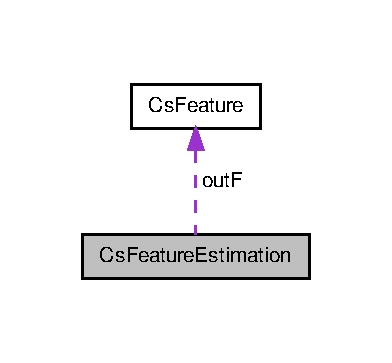
\includegraphics[width=188pt]{class_cs_feature_estimation__coll__graph}
\end{center}
\end{figure}
\subsection*{\-Public \-Member \-Functions}
\begin{DoxyCompactItemize}
\item 
\hyperlink{class_cs_feature_estimation_aa7f0224770d27abed5c151282b0335d5}{\-Cs\-Feature\-Estimation} ()
\item 
\hyperlink{class_cs_feature_estimation_afc2f51c2f489b8290900643e011f06df}{$\sim$\-Cs\-Feature\-Estimation} ()
\item 
void \hyperlink{class_cs_feature_estimation_ad32a35aa8166ab63e7fdececc2ec313a}{init\-Box} (\hyperlink{common_8h_a36884aa4a3c181fa4c284d79329ad166}{\-Cloud\-Ptr} \&cloud)
\item 
\hyperlink{class_cs_feature}{\-Cs\-Feature} \hyperlink{class_cs_feature_estimation_ae3c58e0d970953a13cbd2b250193a297}{compute} (\hyperlink{common_8h_a36884aa4a3c181fa4c284d79329ad166}{\-Cloud\-Ptr} \&cloud)
\item 
float \hyperlink{class_cs_feature_estimation_a87416044424af9e1282e68ec43e4c2d6}{eval\-One\-Point} (\hyperlink{common_8h_af63aa02ad22799ec1b392e97942874b5}{\-Point\-T} pt)
\end{DoxyCompactItemize}
\subsection*{\-Public \-Attributes}
\begin{DoxyCompactItemize}
\item 
\-Vector4f \hyperlink{class_cs_feature_estimation_a97a02375d6a8869f419db0444f6d7252}{m\-\_\-box\-Min}
\item 
\-Vector4f \hyperlink{class_cs_feature_estimation_ad9ed40ac0baf36fe5f1624883baca315}{m\-\_\-box\-Max}
\item 
\hyperlink{common_8h_a36884aa4a3c181fa4c284d79329ad166}{\-Cloud\-Ptr} \hyperlink{class_cs_feature_estimation_a7814bdaf2ec7ee028bb381e9e920fe85}{m\-\_\-keypoints}
\item 
int \hyperlink{class_cs_feature_estimation_a236193badf883b6eff1bbeb4868734a2}{m\-\_\-key\-Size}
\item 
\hyperlink{class_cs_feature}{\-Cs\-Feature} \hyperlink{class_cs_feature_estimation_ae23cbdd6bb125898febbc39c86fe6ed7}{out\-F}
\item 
float \hyperlink{class_cs_feature_estimation_acca08a432c066c2514d345cb9b5976b9}{m\-\_\-gridsize}
\item 
int \hyperlink{class_cs_feature_estimation_a594822f84ee39bbe6f16dad384459fea}{m\-\_\-x\-Nr}
\item 
int \hyperlink{class_cs_feature_estimation_a80110aa818455b337bcde0bbb3cf07be}{m\-\_\-y\-Nr}
\item 
int \hyperlink{class_cs_feature_estimation_a7f984e61208d61e119f78003b3cebd99}{m\-\_\-z\-Nr}
\item 
int \hyperlink{class_cs_feature_estimation_a1bd986e4871bb35f951274418e4dddaf}{m\-\_\-grid\-Nr}
\end{DoxyCompactItemize}


\subsection{\-Constructor \& \-Destructor \-Documentation}
\hypertarget{class_cs_feature_estimation_aa7f0224770d27abed5c151282b0335d5}{\index{\-Cs\-Feature\-Estimation@{\-Cs\-Feature\-Estimation}!\-Cs\-Feature\-Estimation@{\-Cs\-Feature\-Estimation}}
\index{\-Cs\-Feature\-Estimation@{\-Cs\-Feature\-Estimation}!CsFeatureEstimation@{\-Cs\-Feature\-Estimation}}
\subsubsection[{\-Cs\-Feature\-Estimation}]{\setlength{\rightskip}{0pt plus 5cm}{\bf \-Cs\-Feature\-Estimation\-::\-Cs\-Feature\-Estimation} (
\begin{DoxyParamCaption}
{}
\end{DoxyParamCaption}
)}}\label{class_cs_feature_estimation_aa7f0224770d27abed5c151282b0335d5}
\hypertarget{class_cs_feature_estimation_afc2f51c2f489b8290900643e011f06df}{\index{\-Cs\-Feature\-Estimation@{\-Cs\-Feature\-Estimation}!$\sim$\-Cs\-Feature\-Estimation@{$\sim$\-Cs\-Feature\-Estimation}}
\index{$\sim$\-Cs\-Feature\-Estimation@{$\sim$\-Cs\-Feature\-Estimation}!CsFeatureEstimation@{\-Cs\-Feature\-Estimation}}
\subsubsection[{$\sim$\-Cs\-Feature\-Estimation}]{\setlength{\rightskip}{0pt plus 5cm}{\bf \-Cs\-Feature\-Estimation\-::$\sim$\-Cs\-Feature\-Estimation} (
\begin{DoxyParamCaption}
{}
\end{DoxyParamCaption}
)}}\label{class_cs_feature_estimation_afc2f51c2f489b8290900643e011f06df}


\subsection{\-Member \-Function \-Documentation}
\hypertarget{class_cs_feature_estimation_ae3c58e0d970953a13cbd2b250193a297}{\index{\-Cs\-Feature\-Estimation@{\-Cs\-Feature\-Estimation}!compute@{compute}}
\index{compute@{compute}!CsFeatureEstimation@{\-Cs\-Feature\-Estimation}}
\subsubsection[{compute}]{\setlength{\rightskip}{0pt plus 5cm}{\bf \-Cs\-Feature} {\bf \-Cs\-Feature\-Estimation\-::compute} (
\begin{DoxyParamCaption}
\item[{{\bf \-Cloud\-Ptr} \&}]{cloud}
\end{DoxyParamCaption}
)}}\label{class_cs_feature_estimation_ae3c58e0d970953a13cbd2b250193a297}


\-Here is the call graph for this function\-:
\nopagebreak
\begin{figure}[H]
\begin{center}
\leavevmode
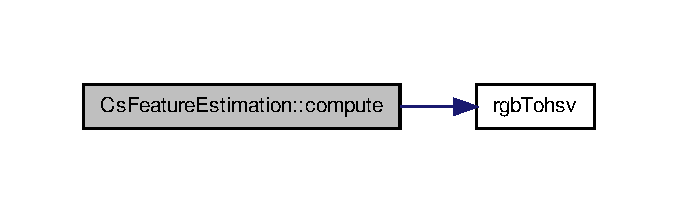
\includegraphics[width=326pt]{class_cs_feature_estimation_ae3c58e0d970953a13cbd2b250193a297_cgraph}
\end{center}
\end{figure}


\hypertarget{class_cs_feature_estimation_a87416044424af9e1282e68ec43e4c2d6}{\index{\-Cs\-Feature\-Estimation@{\-Cs\-Feature\-Estimation}!eval\-One\-Point@{eval\-One\-Point}}
\index{eval\-One\-Point@{eval\-One\-Point}!CsFeatureEstimation@{\-Cs\-Feature\-Estimation}}
\subsubsection[{eval\-One\-Point}]{\setlength{\rightskip}{0pt plus 5cm}float {\bf \-Cs\-Feature\-Estimation\-::eval\-One\-Point} (
\begin{DoxyParamCaption}
\item[{{\bf \-Point\-T}}]{pt}
\end{DoxyParamCaption}
)}}\label{class_cs_feature_estimation_a87416044424af9e1282e68ec43e4c2d6}


\-Here is the call graph for this function\-:
\nopagebreak
\begin{figure}[H]
\begin{center}
\leavevmode
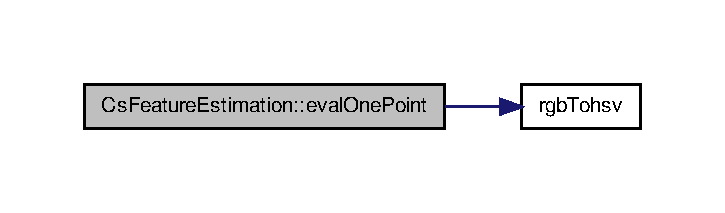
\includegraphics[width=348pt]{class_cs_feature_estimation_a87416044424af9e1282e68ec43e4c2d6_cgraph}
\end{center}
\end{figure}


\hypertarget{class_cs_feature_estimation_ad32a35aa8166ab63e7fdececc2ec313a}{\index{\-Cs\-Feature\-Estimation@{\-Cs\-Feature\-Estimation}!init\-Box@{init\-Box}}
\index{init\-Box@{init\-Box}!CsFeatureEstimation@{\-Cs\-Feature\-Estimation}}
\subsubsection[{init\-Box}]{\setlength{\rightskip}{0pt plus 5cm}void {\bf \-Cs\-Feature\-Estimation\-::init\-Box} (
\begin{DoxyParamCaption}
\item[{{\bf \-Cloud\-Ptr} \&}]{cloud}
\end{DoxyParamCaption}
)}}\label{class_cs_feature_estimation_ad32a35aa8166ab63e7fdececc2ec313a}


\subsection{\-Member \-Data \-Documentation}
\hypertarget{class_cs_feature_estimation_ad9ed40ac0baf36fe5f1624883baca315}{\index{\-Cs\-Feature\-Estimation@{\-Cs\-Feature\-Estimation}!m\-\_\-box\-Max@{m\-\_\-box\-Max}}
\index{m\-\_\-box\-Max@{m\-\_\-box\-Max}!CsFeatureEstimation@{\-Cs\-Feature\-Estimation}}
\subsubsection[{m\-\_\-box\-Max}]{\setlength{\rightskip}{0pt plus 5cm}\-Vector4f {\bf \-Cs\-Feature\-Estimation\-::m\-\_\-box\-Max}}}\label{class_cs_feature_estimation_ad9ed40ac0baf36fe5f1624883baca315}
\hypertarget{class_cs_feature_estimation_a97a02375d6a8869f419db0444f6d7252}{\index{\-Cs\-Feature\-Estimation@{\-Cs\-Feature\-Estimation}!m\-\_\-box\-Min@{m\-\_\-box\-Min}}
\index{m\-\_\-box\-Min@{m\-\_\-box\-Min}!CsFeatureEstimation@{\-Cs\-Feature\-Estimation}}
\subsubsection[{m\-\_\-box\-Min}]{\setlength{\rightskip}{0pt plus 5cm}\-Vector4f {\bf \-Cs\-Feature\-Estimation\-::m\-\_\-box\-Min}}}\label{class_cs_feature_estimation_a97a02375d6a8869f419db0444f6d7252}
\hypertarget{class_cs_feature_estimation_a1bd986e4871bb35f951274418e4dddaf}{\index{\-Cs\-Feature\-Estimation@{\-Cs\-Feature\-Estimation}!m\-\_\-grid\-Nr@{m\-\_\-grid\-Nr}}
\index{m\-\_\-grid\-Nr@{m\-\_\-grid\-Nr}!CsFeatureEstimation@{\-Cs\-Feature\-Estimation}}
\subsubsection[{m\-\_\-grid\-Nr}]{\setlength{\rightskip}{0pt plus 5cm}int {\bf \-Cs\-Feature\-Estimation\-::m\-\_\-grid\-Nr}}}\label{class_cs_feature_estimation_a1bd986e4871bb35f951274418e4dddaf}
\hypertarget{class_cs_feature_estimation_acca08a432c066c2514d345cb9b5976b9}{\index{\-Cs\-Feature\-Estimation@{\-Cs\-Feature\-Estimation}!m\-\_\-gridsize@{m\-\_\-gridsize}}
\index{m\-\_\-gridsize@{m\-\_\-gridsize}!CsFeatureEstimation@{\-Cs\-Feature\-Estimation}}
\subsubsection[{m\-\_\-gridsize}]{\setlength{\rightskip}{0pt plus 5cm}float {\bf \-Cs\-Feature\-Estimation\-::m\-\_\-gridsize}}}\label{class_cs_feature_estimation_acca08a432c066c2514d345cb9b5976b9}
\hypertarget{class_cs_feature_estimation_a7814bdaf2ec7ee028bb381e9e920fe85}{\index{\-Cs\-Feature\-Estimation@{\-Cs\-Feature\-Estimation}!m\-\_\-keypoints@{m\-\_\-keypoints}}
\index{m\-\_\-keypoints@{m\-\_\-keypoints}!CsFeatureEstimation@{\-Cs\-Feature\-Estimation}}
\subsubsection[{m\-\_\-keypoints}]{\setlength{\rightskip}{0pt plus 5cm}{\bf \-Cloud\-Ptr} {\bf \-Cs\-Feature\-Estimation\-::m\-\_\-keypoints}}}\label{class_cs_feature_estimation_a7814bdaf2ec7ee028bb381e9e920fe85}
\hypertarget{class_cs_feature_estimation_a236193badf883b6eff1bbeb4868734a2}{\index{\-Cs\-Feature\-Estimation@{\-Cs\-Feature\-Estimation}!m\-\_\-key\-Size@{m\-\_\-key\-Size}}
\index{m\-\_\-key\-Size@{m\-\_\-key\-Size}!CsFeatureEstimation@{\-Cs\-Feature\-Estimation}}
\subsubsection[{m\-\_\-key\-Size}]{\setlength{\rightskip}{0pt plus 5cm}int {\bf \-Cs\-Feature\-Estimation\-::m\-\_\-key\-Size}}}\label{class_cs_feature_estimation_a236193badf883b6eff1bbeb4868734a2}
\hypertarget{class_cs_feature_estimation_a594822f84ee39bbe6f16dad384459fea}{\index{\-Cs\-Feature\-Estimation@{\-Cs\-Feature\-Estimation}!m\-\_\-x\-Nr@{m\-\_\-x\-Nr}}
\index{m\-\_\-x\-Nr@{m\-\_\-x\-Nr}!CsFeatureEstimation@{\-Cs\-Feature\-Estimation}}
\subsubsection[{m\-\_\-x\-Nr}]{\setlength{\rightskip}{0pt plus 5cm}int {\bf \-Cs\-Feature\-Estimation\-::m\-\_\-x\-Nr}}}\label{class_cs_feature_estimation_a594822f84ee39bbe6f16dad384459fea}
\hypertarget{class_cs_feature_estimation_a80110aa818455b337bcde0bbb3cf07be}{\index{\-Cs\-Feature\-Estimation@{\-Cs\-Feature\-Estimation}!m\-\_\-y\-Nr@{m\-\_\-y\-Nr}}
\index{m\-\_\-y\-Nr@{m\-\_\-y\-Nr}!CsFeatureEstimation@{\-Cs\-Feature\-Estimation}}
\subsubsection[{m\-\_\-y\-Nr}]{\setlength{\rightskip}{0pt plus 5cm}int {\bf \-Cs\-Feature\-Estimation\-::m\-\_\-y\-Nr}}}\label{class_cs_feature_estimation_a80110aa818455b337bcde0bbb3cf07be}
\hypertarget{class_cs_feature_estimation_a7f984e61208d61e119f78003b3cebd99}{\index{\-Cs\-Feature\-Estimation@{\-Cs\-Feature\-Estimation}!m\-\_\-z\-Nr@{m\-\_\-z\-Nr}}
\index{m\-\_\-z\-Nr@{m\-\_\-z\-Nr}!CsFeatureEstimation@{\-Cs\-Feature\-Estimation}}
\subsubsection[{m\-\_\-z\-Nr}]{\setlength{\rightskip}{0pt plus 5cm}int {\bf \-Cs\-Feature\-Estimation\-::m\-\_\-z\-Nr}}}\label{class_cs_feature_estimation_a7f984e61208d61e119f78003b3cebd99}
\hypertarget{class_cs_feature_estimation_ae23cbdd6bb125898febbc39c86fe6ed7}{\index{\-Cs\-Feature\-Estimation@{\-Cs\-Feature\-Estimation}!out\-F@{out\-F}}
\index{out\-F@{out\-F}!CsFeatureEstimation@{\-Cs\-Feature\-Estimation}}
\subsubsection[{out\-F}]{\setlength{\rightskip}{0pt plus 5cm}{\bf \-Cs\-Feature} {\bf \-Cs\-Feature\-Estimation\-::out\-F}}}\label{class_cs_feature_estimation_ae23cbdd6bb125898febbc39c86fe6ed7}


\-The documentation for this class was generated from the following files\-:\begin{DoxyCompactItemize}
\item 
/home/koosy/koosywork/pmot\-\_\-realtime/pmot\-\_\-realtime/src/\hyperlink{csfeature_8h}{csfeature.\-h}\item 
/home/koosy/koosywork/pmot\-\_\-realtime/pmot\-\_\-realtime/src/\hyperlink{csfeature_8cpp}{csfeature.\-cpp}\end{DoxyCompactItemize}

\hypertarget{class_c_s_g_p_u}{\section{\-C\-S\-G\-P\-U \-Class \-Reference}
\label{class_c_s_g_p_u}\index{\-C\-S\-G\-P\-U@{\-C\-S\-G\-P\-U}}
}


{\ttfamily \#include $<$csgpu.\-h$>$}

\subsection*{\-Public \-Member \-Functions}
\begin{DoxyCompactItemize}
\item 
\hyperlink{class_c_s_g_p_u_a24d5da075a7960654334096ecbfdb49b}{\-C\-S\-G\-P\-U} ()
\item 
\hyperlink{class_c_s_g_p_u_a8443e5cf8518155df3f7ff7adff5fcec}{\-C\-S\-G\-P\-U} (float gridsize\-\_\-, int xnr\-\_\-, int ynr\-\_\-, int znr\-\_\-, int partnr\-\_\-, int cloudsize\-\_\-)
\item 
\hyperlink{class_c_s_g_p_u_a4a1672b4a09d646872ddeb4e7edf805a}{$\sim$\-C\-S\-G\-P\-U} ()
\item 
std\-::vector$<$ float $>$ \hyperlink{class_c_s_g_p_u_a23ff255887244e1307b41a657e5e26f5}{compute} ()
\end{DoxyCompactItemize}
\subsection*{\-Public \-Attributes}
\begin{DoxyCompactItemize}
\item 
int \hyperlink{class_c_s_g_p_u_a8b544902a5b4fe5f7e010dda96ce7e93}{aa}
\item 
int \hyperlink{class_c_s_g_p_u_ace2257bc4c7eb29735ee01c03b7a7471}{histsize}
\item 
size\-\_\-t \hyperlink{class_c_s_g_p_u_a70716430b4cdd6085222556ef8ef2fb0}{part\-Nr}
\item 
size\-\_\-t \hyperlink{class_c_s_g_p_u_a3e3845d161dfaf5087e1a9329f0795cb}{cloud\-Size}
\item 
size\-\_\-t \hyperlink{class_c_s_g_p_u_aca9cc9e5ae863e7395d053ad724184da}{refcloud\-Size}
\item 
size\-\_\-t \hyperlink{class_c_s_g_p_u_a8f232965ca3bfd56b6d96ea5b9d92a57}{x\-Nr}
\item 
size\-\_\-t \hyperlink{class_c_s_g_p_u_a432972a16b011b3f0733b0e88185d8c9}{y\-Nr}
\item 
size\-\_\-t \hyperlink{class_c_s_g_p_u_a628e566c47edc244f4ced4ea8fdff40c}{z\-Nr}
\item 
float3 \hyperlink{class_c_s_g_p_u_a546cfd9fd17e125e8c1c7530b0783057}{min\-Pt}
\item 
float3 \hyperlink{class_c_s_g_p_u_a43d5d65a62bdd4c0529a7c5597526573}{max\-Pt}
\item 
float \hyperlink{class_c_s_g_p_u_a819ee6c0a3e2733e3edc350f9e090d39}{gridsize}
\item 
float $\ast$ \hyperlink{class_c_s_g_p_u_a8f0488218cd59487bb4900c066e5e250}{refhist}
\item 
float3 $\ast$ \hyperlink{class_c_s_g_p_u_aae0654f6af8886eeef6a455efbc1e1ed}{cloudpos}
\item 
float3 $\ast$ \hyperlink{class_c_s_g_p_u_a16a0b4b64cd6b658b618ddab15e4106a}{cloudhsv}
\item 
float3 $\ast$ \hyperlink{class_c_s_g_p_u_a6342a509f62d97d425b4759804872107}{refcloud}
\item 
float3 $\ast$ \hyperlink{class_c_s_g_p_u_aa654de3881bb51f6d9f461955976ac00}{partpos}
\item 
float3 $\ast$ \hyperlink{class_c_s_g_p_u_a832b559fdd18b22c2705d4ffa5c0d93d}{partrot}
\end{DoxyCompactItemize}


\subsection{\-Constructor \& \-Destructor \-Documentation}
\hypertarget{class_c_s_g_p_u_a24d5da075a7960654334096ecbfdb49b}{\index{\-C\-S\-G\-P\-U@{\-C\-S\-G\-P\-U}!\-C\-S\-G\-P\-U@{\-C\-S\-G\-P\-U}}
\index{\-C\-S\-G\-P\-U@{\-C\-S\-G\-P\-U}!CSGPU@{\-C\-S\-G\-P\-U}}
\subsubsection[{\-C\-S\-G\-P\-U}]{\setlength{\rightskip}{0pt plus 5cm}{\bf \-C\-S\-G\-P\-U\-::\-C\-S\-G\-P\-U} (
\begin{DoxyParamCaption}
{}
\end{DoxyParamCaption}
)\hspace{0.3cm}{\ttfamily  \mbox{[}inline\mbox{]}}}}\label{class_c_s_g_p_u_a24d5da075a7960654334096ecbfdb49b}
\hypertarget{class_c_s_g_p_u_a8443e5cf8518155df3f7ff7adff5fcec}{\index{\-C\-S\-G\-P\-U@{\-C\-S\-G\-P\-U}!\-C\-S\-G\-P\-U@{\-C\-S\-G\-P\-U}}
\index{\-C\-S\-G\-P\-U@{\-C\-S\-G\-P\-U}!CSGPU@{\-C\-S\-G\-P\-U}}
\subsubsection[{\-C\-S\-G\-P\-U}]{\setlength{\rightskip}{0pt plus 5cm}{\bf \-C\-S\-G\-P\-U\-::\-C\-S\-G\-P\-U} (
\begin{DoxyParamCaption}
\item[{float}]{gridsize\-\_\-, }
\item[{int}]{xnr\-\_\-, }
\item[{int}]{ynr\-\_\-, }
\item[{int}]{znr\-\_\-, }
\item[{int}]{partnr\-\_\-, }
\item[{int}]{cloudsize\-\_\-}
\end{DoxyParamCaption}
)\hspace{0.3cm}{\ttfamily  \mbox{[}inline\mbox{]}}}}\label{class_c_s_g_p_u_a8443e5cf8518155df3f7ff7adff5fcec}
\hypertarget{class_c_s_g_p_u_a4a1672b4a09d646872ddeb4e7edf805a}{\index{\-C\-S\-G\-P\-U@{\-C\-S\-G\-P\-U}!$\sim$\-C\-S\-G\-P\-U@{$\sim$\-C\-S\-G\-P\-U}}
\index{$\sim$\-C\-S\-G\-P\-U@{$\sim$\-C\-S\-G\-P\-U}!CSGPU@{\-C\-S\-G\-P\-U}}
\subsubsection[{$\sim$\-C\-S\-G\-P\-U}]{\setlength{\rightskip}{0pt plus 5cm}{\bf \-C\-S\-G\-P\-U\-::$\sim$\-C\-S\-G\-P\-U} (
\begin{DoxyParamCaption}
{}
\end{DoxyParamCaption}
)\hspace{0.3cm}{\ttfamily  \mbox{[}inline\mbox{]}}}}\label{class_c_s_g_p_u_a4a1672b4a09d646872ddeb4e7edf805a}


\subsection{\-Member \-Function \-Documentation}
\hypertarget{class_c_s_g_p_u_a23ff255887244e1307b41a657e5e26f5}{\index{\-C\-S\-G\-P\-U@{\-C\-S\-G\-P\-U}!compute@{compute}}
\index{compute@{compute}!CSGPU@{\-C\-S\-G\-P\-U}}
\subsubsection[{compute}]{\setlength{\rightskip}{0pt plus 5cm}std\-::vector$<$float$>$ {\bf \-C\-S\-G\-P\-U\-::compute} (
\begin{DoxyParamCaption}
{}
\end{DoxyParamCaption}
)}}\label{class_c_s_g_p_u_a23ff255887244e1307b41a657e5e26f5}


\subsection{\-Member \-Data \-Documentation}
\hypertarget{class_c_s_g_p_u_a8b544902a5b4fe5f7e010dda96ce7e93}{\index{\-C\-S\-G\-P\-U@{\-C\-S\-G\-P\-U}!aa@{aa}}
\index{aa@{aa}!CSGPU@{\-C\-S\-G\-P\-U}}
\subsubsection[{aa}]{\setlength{\rightskip}{0pt plus 5cm}int {\bf \-C\-S\-G\-P\-U\-::aa}}}\label{class_c_s_g_p_u_a8b544902a5b4fe5f7e010dda96ce7e93}
\hypertarget{class_c_s_g_p_u_a16a0b4b64cd6b658b618ddab15e4106a}{\index{\-C\-S\-G\-P\-U@{\-C\-S\-G\-P\-U}!cloudhsv@{cloudhsv}}
\index{cloudhsv@{cloudhsv}!CSGPU@{\-C\-S\-G\-P\-U}}
\subsubsection[{cloudhsv}]{\setlength{\rightskip}{0pt plus 5cm}float3$\ast$ {\bf \-C\-S\-G\-P\-U\-::cloudhsv}}}\label{class_c_s_g_p_u_a16a0b4b64cd6b658b618ddab15e4106a}
\hypertarget{class_c_s_g_p_u_aae0654f6af8886eeef6a455efbc1e1ed}{\index{\-C\-S\-G\-P\-U@{\-C\-S\-G\-P\-U}!cloudpos@{cloudpos}}
\index{cloudpos@{cloudpos}!CSGPU@{\-C\-S\-G\-P\-U}}
\subsubsection[{cloudpos}]{\setlength{\rightskip}{0pt plus 5cm}float3$\ast$ {\bf \-C\-S\-G\-P\-U\-::cloudpos}}}\label{class_c_s_g_p_u_aae0654f6af8886eeef6a455efbc1e1ed}
\hypertarget{class_c_s_g_p_u_a3e3845d161dfaf5087e1a9329f0795cb}{\index{\-C\-S\-G\-P\-U@{\-C\-S\-G\-P\-U}!cloud\-Size@{cloud\-Size}}
\index{cloud\-Size@{cloud\-Size}!CSGPU@{\-C\-S\-G\-P\-U}}
\subsubsection[{cloud\-Size}]{\setlength{\rightskip}{0pt plus 5cm}size\-\_\-t {\bf \-C\-S\-G\-P\-U\-::cloud\-Size}}}\label{class_c_s_g_p_u_a3e3845d161dfaf5087e1a9329f0795cb}
\hypertarget{class_c_s_g_p_u_a819ee6c0a3e2733e3edc350f9e090d39}{\index{\-C\-S\-G\-P\-U@{\-C\-S\-G\-P\-U}!gridsize@{gridsize}}
\index{gridsize@{gridsize}!CSGPU@{\-C\-S\-G\-P\-U}}
\subsubsection[{gridsize}]{\setlength{\rightskip}{0pt plus 5cm}float {\bf \-C\-S\-G\-P\-U\-::gridsize}}}\label{class_c_s_g_p_u_a819ee6c0a3e2733e3edc350f9e090d39}
\hypertarget{class_c_s_g_p_u_ace2257bc4c7eb29735ee01c03b7a7471}{\index{\-C\-S\-G\-P\-U@{\-C\-S\-G\-P\-U}!histsize@{histsize}}
\index{histsize@{histsize}!CSGPU@{\-C\-S\-G\-P\-U}}
\subsubsection[{histsize}]{\setlength{\rightskip}{0pt plus 5cm}int {\bf \-C\-S\-G\-P\-U\-::histsize}}}\label{class_c_s_g_p_u_ace2257bc4c7eb29735ee01c03b7a7471}
\hypertarget{class_c_s_g_p_u_a43d5d65a62bdd4c0529a7c5597526573}{\index{\-C\-S\-G\-P\-U@{\-C\-S\-G\-P\-U}!max\-Pt@{max\-Pt}}
\index{max\-Pt@{max\-Pt}!CSGPU@{\-C\-S\-G\-P\-U}}
\subsubsection[{max\-Pt}]{\setlength{\rightskip}{0pt plus 5cm}float3 {\bf \-C\-S\-G\-P\-U\-::max\-Pt}}}\label{class_c_s_g_p_u_a43d5d65a62bdd4c0529a7c5597526573}
\hypertarget{class_c_s_g_p_u_a546cfd9fd17e125e8c1c7530b0783057}{\index{\-C\-S\-G\-P\-U@{\-C\-S\-G\-P\-U}!min\-Pt@{min\-Pt}}
\index{min\-Pt@{min\-Pt}!CSGPU@{\-C\-S\-G\-P\-U}}
\subsubsection[{min\-Pt}]{\setlength{\rightskip}{0pt plus 5cm}float3 {\bf \-C\-S\-G\-P\-U\-::min\-Pt}}}\label{class_c_s_g_p_u_a546cfd9fd17e125e8c1c7530b0783057}
\hypertarget{class_c_s_g_p_u_a70716430b4cdd6085222556ef8ef2fb0}{\index{\-C\-S\-G\-P\-U@{\-C\-S\-G\-P\-U}!part\-Nr@{part\-Nr}}
\index{part\-Nr@{part\-Nr}!CSGPU@{\-C\-S\-G\-P\-U}}
\subsubsection[{part\-Nr}]{\setlength{\rightskip}{0pt plus 5cm}size\-\_\-t {\bf \-C\-S\-G\-P\-U\-::part\-Nr}}}\label{class_c_s_g_p_u_a70716430b4cdd6085222556ef8ef2fb0}
\hypertarget{class_c_s_g_p_u_aa654de3881bb51f6d9f461955976ac00}{\index{\-C\-S\-G\-P\-U@{\-C\-S\-G\-P\-U}!partpos@{partpos}}
\index{partpos@{partpos}!CSGPU@{\-C\-S\-G\-P\-U}}
\subsubsection[{partpos}]{\setlength{\rightskip}{0pt plus 5cm}float3$\ast$ {\bf \-C\-S\-G\-P\-U\-::partpos}}}\label{class_c_s_g_p_u_aa654de3881bb51f6d9f461955976ac00}
\hypertarget{class_c_s_g_p_u_a832b559fdd18b22c2705d4ffa5c0d93d}{\index{\-C\-S\-G\-P\-U@{\-C\-S\-G\-P\-U}!partrot@{partrot}}
\index{partrot@{partrot}!CSGPU@{\-C\-S\-G\-P\-U}}
\subsubsection[{partrot}]{\setlength{\rightskip}{0pt plus 5cm}float3$\ast$ {\bf \-C\-S\-G\-P\-U\-::partrot}}}\label{class_c_s_g_p_u_a832b559fdd18b22c2705d4ffa5c0d93d}
\hypertarget{class_c_s_g_p_u_a6342a509f62d97d425b4759804872107}{\index{\-C\-S\-G\-P\-U@{\-C\-S\-G\-P\-U}!refcloud@{refcloud}}
\index{refcloud@{refcloud}!CSGPU@{\-C\-S\-G\-P\-U}}
\subsubsection[{refcloud}]{\setlength{\rightskip}{0pt plus 5cm}float3$\ast$ {\bf \-C\-S\-G\-P\-U\-::refcloud}}}\label{class_c_s_g_p_u_a6342a509f62d97d425b4759804872107}
\hypertarget{class_c_s_g_p_u_aca9cc9e5ae863e7395d053ad724184da}{\index{\-C\-S\-G\-P\-U@{\-C\-S\-G\-P\-U}!refcloud\-Size@{refcloud\-Size}}
\index{refcloud\-Size@{refcloud\-Size}!CSGPU@{\-C\-S\-G\-P\-U}}
\subsubsection[{refcloud\-Size}]{\setlength{\rightskip}{0pt plus 5cm}size\-\_\-t {\bf \-C\-S\-G\-P\-U\-::refcloud\-Size}}}\label{class_c_s_g_p_u_aca9cc9e5ae863e7395d053ad724184da}
\hypertarget{class_c_s_g_p_u_a8f0488218cd59487bb4900c066e5e250}{\index{\-C\-S\-G\-P\-U@{\-C\-S\-G\-P\-U}!refhist@{refhist}}
\index{refhist@{refhist}!CSGPU@{\-C\-S\-G\-P\-U}}
\subsubsection[{refhist}]{\setlength{\rightskip}{0pt plus 5cm}float$\ast$ {\bf \-C\-S\-G\-P\-U\-::refhist}}}\label{class_c_s_g_p_u_a8f0488218cd59487bb4900c066e5e250}
\hypertarget{class_c_s_g_p_u_a8f232965ca3bfd56b6d96ea5b9d92a57}{\index{\-C\-S\-G\-P\-U@{\-C\-S\-G\-P\-U}!x\-Nr@{x\-Nr}}
\index{x\-Nr@{x\-Nr}!CSGPU@{\-C\-S\-G\-P\-U}}
\subsubsection[{x\-Nr}]{\setlength{\rightskip}{0pt plus 5cm}size\-\_\-t {\bf \-C\-S\-G\-P\-U\-::x\-Nr}}}\label{class_c_s_g_p_u_a8f232965ca3bfd56b6d96ea5b9d92a57}
\hypertarget{class_c_s_g_p_u_a432972a16b011b3f0733b0e88185d8c9}{\index{\-C\-S\-G\-P\-U@{\-C\-S\-G\-P\-U}!y\-Nr@{y\-Nr}}
\index{y\-Nr@{y\-Nr}!CSGPU@{\-C\-S\-G\-P\-U}}
\subsubsection[{y\-Nr}]{\setlength{\rightskip}{0pt plus 5cm}size\-\_\-t {\bf \-C\-S\-G\-P\-U\-::y\-Nr}}}\label{class_c_s_g_p_u_a432972a16b011b3f0733b0e88185d8c9}
\hypertarget{class_c_s_g_p_u_a628e566c47edc244f4ced4ea8fdff40c}{\index{\-C\-S\-G\-P\-U@{\-C\-S\-G\-P\-U}!z\-Nr@{z\-Nr}}
\index{z\-Nr@{z\-Nr}!CSGPU@{\-C\-S\-G\-P\-U}}
\subsubsection[{z\-Nr}]{\setlength{\rightskip}{0pt plus 5cm}size\-\_\-t {\bf \-C\-S\-G\-P\-U\-::z\-Nr}}}\label{class_c_s_g_p_u_a628e566c47edc244f4ced4ea8fdff40c}


\-The documentation for this class was generated from the following file\-:\begin{DoxyCompactItemize}
\item 
/home/koosy/koosywork/pmot\-\_\-realtime/pmot\-\_\-realtime/src/\hyperlink{csgpu_8h}{csgpu.\-h}\end{DoxyCompactItemize}

\hypertarget{struct_p_c_object_1_1_edge}{\section{\-P\-C\-Object\-:\-:\-Edge \-Struct \-Reference}
\label{struct_p_c_object_1_1_edge}\index{\-P\-C\-Object\-::\-Edge@{\-P\-C\-Object\-::\-Edge}}
}


{\ttfamily \#include $<$pcobject.\-h$>$}



\-Collaboration diagram for \-P\-C\-Object\-:\-:\-Edge\-:
\nopagebreak
\begin{figure}[H]
\begin{center}
\leavevmode
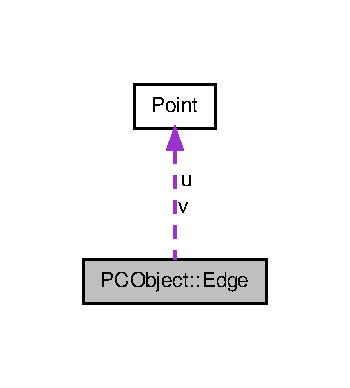
\includegraphics[width=168pt]{struct_p_c_object_1_1_edge__coll__graph}
\end{center}
\end{figure}
\subsection*{\-Public \-Attributes}
\begin{DoxyCompactItemize}
\item 
\hyperlink{class_point}{\-Point} \hyperlink{struct_p_c_object_1_1_edge_af4067d329722069784adbc2e4df9fc73}{u}
\item 
\hyperlink{class_point}{\-Point} \hyperlink{struct_p_c_object_1_1_edge_aaf9714de2de62884dfb6b682f54896f9}{v}
\item 
double \hyperlink{struct_p_c_object_1_1_edge_a5f7ec9c43abe68d31fb305b8344a2e5b}{weight}
\end{DoxyCompactItemize}


\subsection{\-Member \-Data \-Documentation}
\hypertarget{struct_p_c_object_1_1_edge_af4067d329722069784adbc2e4df9fc73}{\index{\-P\-C\-Object\-::\-Edge@{\-P\-C\-Object\-::\-Edge}!u@{u}}
\index{u@{u}!PCObject::Edge@{\-P\-C\-Object\-::\-Edge}}
\subsubsection[{u}]{\setlength{\rightskip}{0pt plus 5cm}{\bf \-Point} {\bf \-P\-C\-Object\-::\-Edge\-::u}}}\label{struct_p_c_object_1_1_edge_af4067d329722069784adbc2e4df9fc73}
\hypertarget{struct_p_c_object_1_1_edge_aaf9714de2de62884dfb6b682f54896f9}{\index{\-P\-C\-Object\-::\-Edge@{\-P\-C\-Object\-::\-Edge}!v@{v}}
\index{v@{v}!PCObject::Edge@{\-P\-C\-Object\-::\-Edge}}
\subsubsection[{v}]{\setlength{\rightskip}{0pt plus 5cm}{\bf \-Point} {\bf \-P\-C\-Object\-::\-Edge\-::v}}}\label{struct_p_c_object_1_1_edge_aaf9714de2de62884dfb6b682f54896f9}
\hypertarget{struct_p_c_object_1_1_edge_a5f7ec9c43abe68d31fb305b8344a2e5b}{\index{\-P\-C\-Object\-::\-Edge@{\-P\-C\-Object\-::\-Edge}!weight@{weight}}
\index{weight@{weight}!PCObject::Edge@{\-P\-C\-Object\-::\-Edge}}
\subsubsection[{weight}]{\setlength{\rightskip}{0pt plus 5cm}double {\bf \-P\-C\-Object\-::\-Edge\-::weight}}}\label{struct_p_c_object_1_1_edge_a5f7ec9c43abe68d31fb305b8344a2e5b}


\-The documentation for this struct was generated from the following file\-:\begin{DoxyCompactItemize}
\item 
/home/koosy/koosywork/pmot\-\_\-realtime/pmot\-\_\-realtime/src/\hyperlink{pcobject_8h}{pcobject.\-h}\end{DoxyCompactItemize}

\hypertarget{struct_p_c_object_1_1_edge__spatial}{\section{\-P\-C\-Object\-:\-:\-Edge\-\_\-spatial \-Struct \-Reference}
\label{struct_p_c_object_1_1_edge__spatial}\index{\-P\-C\-Object\-::\-Edge\-\_\-spatial@{\-P\-C\-Object\-::\-Edge\-\_\-spatial}}
}


{\ttfamily \#include $<$pcobject.\-h$>$}

\subsection*{\-Public \-Attributes}
\begin{DoxyCompactItemize}
\item 
\-List\-Graph\-::\-Node \hyperlink{struct_p_c_object_1_1_edge__spatial_a2d9774f6ad421e7852dee873d267b420}{u}
\item 
\-List\-Graph\-::\-Node \hyperlink{struct_p_c_object_1_1_edge__spatial_ac395ba6d91a7054ea23ad9d5711a44f5}{v}
\item 
double \hyperlink{struct_p_c_object_1_1_edge__spatial_a9c3350fad42237e5eb7cc13f0509a0ce}{weight\-\_\-vel}
\item 
double \hyperlink{struct_p_c_object_1_1_edge__spatial_a1bb24b8152a4c3310f933c041fec1a48}{weight\-\_\-pos}
\end{DoxyCompactItemize}


\subsection{\-Member \-Data \-Documentation}
\hypertarget{struct_p_c_object_1_1_edge__spatial_a2d9774f6ad421e7852dee873d267b420}{\index{\-P\-C\-Object\-::\-Edge\-\_\-spatial@{\-P\-C\-Object\-::\-Edge\-\_\-spatial}!u@{u}}
\index{u@{u}!PCObject::Edge_spatial@{\-P\-C\-Object\-::\-Edge\-\_\-spatial}}
\subsubsection[{u}]{\setlength{\rightskip}{0pt plus 5cm}\-List\-Graph\-::\-Node {\bf \-P\-C\-Object\-::\-Edge\-\_\-spatial\-::u}}}\label{struct_p_c_object_1_1_edge__spatial_a2d9774f6ad421e7852dee873d267b420}
\hypertarget{struct_p_c_object_1_1_edge__spatial_ac395ba6d91a7054ea23ad9d5711a44f5}{\index{\-P\-C\-Object\-::\-Edge\-\_\-spatial@{\-P\-C\-Object\-::\-Edge\-\_\-spatial}!v@{v}}
\index{v@{v}!PCObject::Edge_spatial@{\-P\-C\-Object\-::\-Edge\-\_\-spatial}}
\subsubsection[{v}]{\setlength{\rightskip}{0pt plus 5cm}\-List\-Graph\-::\-Node {\bf \-P\-C\-Object\-::\-Edge\-\_\-spatial\-::v}}}\label{struct_p_c_object_1_1_edge__spatial_ac395ba6d91a7054ea23ad9d5711a44f5}
\hypertarget{struct_p_c_object_1_1_edge__spatial_a1bb24b8152a4c3310f933c041fec1a48}{\index{\-P\-C\-Object\-::\-Edge\-\_\-spatial@{\-P\-C\-Object\-::\-Edge\-\_\-spatial}!weight\-\_\-pos@{weight\-\_\-pos}}
\index{weight\-\_\-pos@{weight\-\_\-pos}!PCObject::Edge_spatial@{\-P\-C\-Object\-::\-Edge\-\_\-spatial}}
\subsubsection[{weight\-\_\-pos}]{\setlength{\rightskip}{0pt plus 5cm}double {\bf \-P\-C\-Object\-::\-Edge\-\_\-spatial\-::weight\-\_\-pos}}}\label{struct_p_c_object_1_1_edge__spatial_a1bb24b8152a4c3310f933c041fec1a48}
\hypertarget{struct_p_c_object_1_1_edge__spatial_a9c3350fad42237e5eb7cc13f0509a0ce}{\index{\-P\-C\-Object\-::\-Edge\-\_\-spatial@{\-P\-C\-Object\-::\-Edge\-\_\-spatial}!weight\-\_\-vel@{weight\-\_\-vel}}
\index{weight\-\_\-vel@{weight\-\_\-vel}!PCObject::Edge_spatial@{\-P\-C\-Object\-::\-Edge\-\_\-spatial}}
\subsubsection[{weight\-\_\-vel}]{\setlength{\rightskip}{0pt plus 5cm}double {\bf \-P\-C\-Object\-::\-Edge\-\_\-spatial\-::weight\-\_\-vel}}}\label{struct_p_c_object_1_1_edge__spatial_a9c3350fad42237e5eb7cc13f0509a0ce}


\-The documentation for this struct was generated from the following file\-:\begin{DoxyCompactItemize}
\item 
/home/koosy/koosywork/pmot\-\_\-realtime/pmot\-\_\-realtime/src/\hyperlink{pcobject_8h}{pcobject.\-h}\end{DoxyCompactItemize}

\hypertarget{struct_false_objects}{\section{\-False\-Objects \-Struct \-Reference}
\label{struct_false_objects}\index{\-False\-Objects@{\-False\-Objects}}
}


{\ttfamily \#include $<$pctracking.\-h$>$}



\-Collaboration diagram for \-False\-Objects\-:
\nopagebreak
\begin{figure}[H]
\begin{center}
\leavevmode
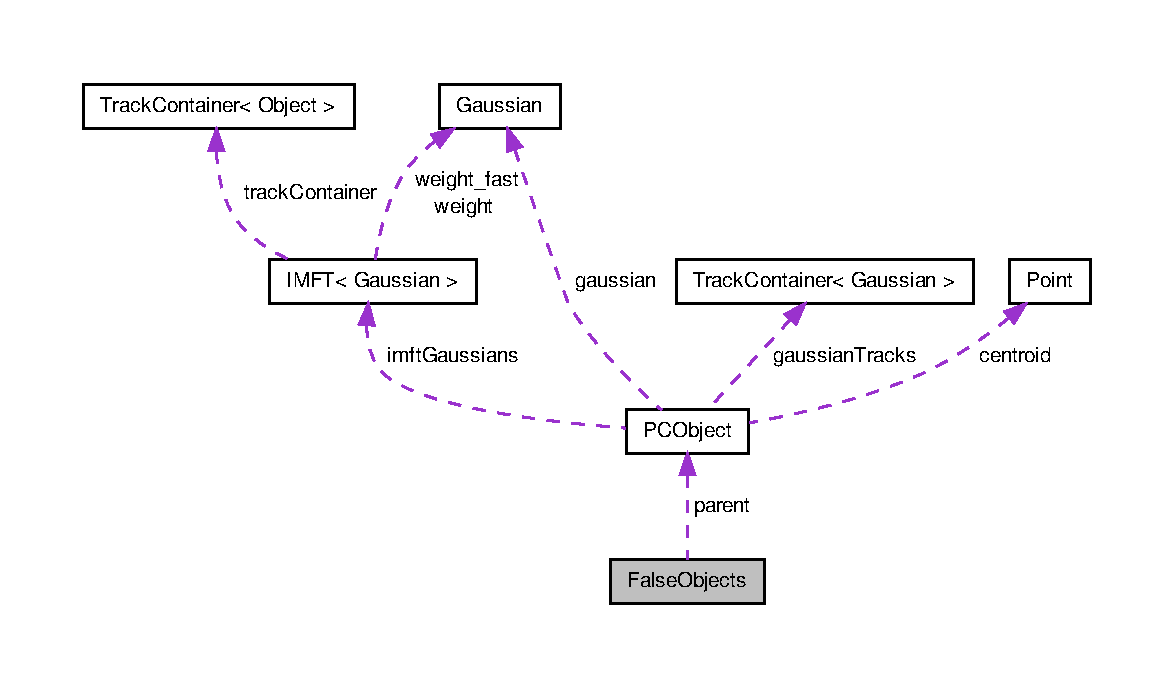
\includegraphics[width=350pt]{struct_false_objects__coll__graph}
\end{center}
\end{figure}
\subsection*{\-Public \-Attributes}
\begin{DoxyCompactItemize}
\item 
\hyperlink{class_p_c_object}{\-P\-C\-Object} \hyperlink{struct_false_objects_a72516a38ec12f2afd7fa072705ba7fd7}{parent}
\item 
vector$<$ \hyperlink{class_p_c_object}{\-P\-C\-Object} $>$ \hyperlink{struct_false_objects_a92ed26914ae6e1b3b628418e13eca43d}{childs}
\end{DoxyCompactItemize}


\subsection{\-Member \-Data \-Documentation}
\hypertarget{struct_false_objects_a92ed26914ae6e1b3b628418e13eca43d}{\index{\-False\-Objects@{\-False\-Objects}!childs@{childs}}
\index{childs@{childs}!FalseObjects@{\-False\-Objects}}
\subsubsection[{childs}]{\setlength{\rightskip}{0pt plus 5cm}vector$<${\bf \-P\-C\-Object}$>$ {\bf \-False\-Objects\-::childs}}}\label{struct_false_objects_a92ed26914ae6e1b3b628418e13eca43d}
\hypertarget{struct_false_objects_a72516a38ec12f2afd7fa072705ba7fd7}{\index{\-False\-Objects@{\-False\-Objects}!parent@{parent}}
\index{parent@{parent}!FalseObjects@{\-False\-Objects}}
\subsubsection[{parent}]{\setlength{\rightskip}{0pt plus 5cm}{\bf \-P\-C\-Object} {\bf \-False\-Objects\-::parent}}}\label{struct_false_objects_a72516a38ec12f2afd7fa072705ba7fd7}


\-The documentation for this struct was generated from the following file\-:\begin{DoxyCompactItemize}
\item 
/home/koosy/koosywork/pmot\-\_\-realtime/pmot\-\_\-realtime/src/\hyperlink{pctracking_8h}{pctracking.\-h}\end{DoxyCompactItemize}

\hypertarget{struct_frame}{\section{\-Frame \-Struct \-Reference}
\label{struct_frame}\index{\-Frame@{\-Frame}}
}


{\ttfamily \#include $<$pctracking.\-h$>$}

\subsection*{\-Public \-Attributes}
\begin{DoxyCompactItemize}
\item 
vector$<$ \hyperlink{struct_track_point}{\-Track\-Point} $>$ \hyperlink{struct_frame_a7c3e2c360430d7c57f9c278aa5d2a7df}{track\-Points}
\item 
int \hyperlink{struct_frame_a08231d06b0a2f5074fa7f4128168a9c0}{time}
\end{DoxyCompactItemize}


\subsection{\-Member \-Data \-Documentation}
\hypertarget{struct_frame_a08231d06b0a2f5074fa7f4128168a9c0}{\index{\-Frame@{\-Frame}!time@{time}}
\index{time@{time}!Frame@{\-Frame}}
\subsubsection[{time}]{\setlength{\rightskip}{0pt plus 5cm}int {\bf \-Frame\-::time}}}\label{struct_frame_a08231d06b0a2f5074fa7f4128168a9c0}
\hypertarget{struct_frame_a7c3e2c360430d7c57f9c278aa5d2a7df}{\index{\-Frame@{\-Frame}!track\-Points@{track\-Points}}
\index{track\-Points@{track\-Points}!Frame@{\-Frame}}
\subsubsection[{track\-Points}]{\setlength{\rightskip}{0pt plus 5cm}vector$<${\bf \-Track\-Point}$>$ {\bf \-Frame\-::track\-Points}}}\label{struct_frame_a7c3e2c360430d7c57f9c278aa5d2a7df}


\-The documentation for this struct was generated from the following file\-:\begin{DoxyCompactItemize}
\item 
/home/koosy/koosywork/pmot\-\_\-realtime/pmot\-\_\-realtime/src/\hyperlink{pctracking_8h}{pctracking.\-h}\end{DoxyCompactItemize}

\hypertarget{struct_track_1_1_frame}{\section{\-Track$<$ \-Object $>$\-:\-:\-Frame \-Struct \-Reference}
\label{struct_track_1_1_frame}\index{\-Track$<$ Object $>$\-::\-Frame@{\-Track$<$ Object $>$\-::\-Frame}}
}


{\ttfamily \#include $<$track.\-h$>$}



\-Collaboration diagram for \-Track$<$ \-Object $>$\-:\-:\-Frame\-:
\nopagebreak
\begin{figure}[H]
\begin{center}
\leavevmode
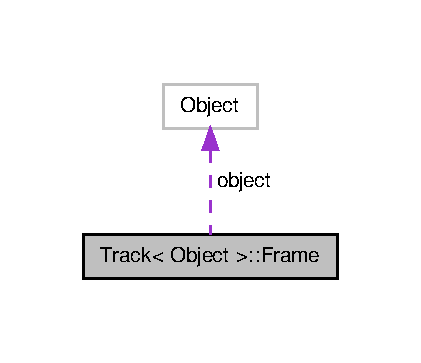
\includegraphics[width=202pt]{struct_track_1_1_frame__coll__graph}
\end{center}
\end{figure}
\subsection*{\-Public \-Attributes}
\begin{DoxyCompactItemize}
\item 
\-Object \hyperlink{struct_track_1_1_frame_a6bbfe33bfab1011aaddd49d35e0ecfb4}{object}
\item 
int \hyperlink{struct_track_1_1_frame_a00cdf6a5e1c6eae134547cd386c8ebd3}{id}
\item 
int \hyperlink{struct_track_1_1_frame_a72677957f8d88952d44074e0af30b624}{time}
\end{DoxyCompactItemize}
\subsubsection*{template$<$class Object$>$ struct Track$<$ Object $>$\-::\-Frame}



\subsection{\-Member \-Data \-Documentation}
\hypertarget{struct_track_1_1_frame_a00cdf6a5e1c6eae134547cd386c8ebd3}{\index{\-Track\-::\-Frame@{\-Track\-::\-Frame}!id@{id}}
\index{id@{id}!Track::Frame@{\-Track\-::\-Frame}}
\subsubsection[{id}]{\setlength{\rightskip}{0pt plus 5cm}template$<$class Object $>$ int {\bf \-Track}$<$ \-Object $>$\-::{\bf \-Frame\-::id}}}\label{struct_track_1_1_frame_a00cdf6a5e1c6eae134547cd386c8ebd3}
\hypertarget{struct_track_1_1_frame_a6bbfe33bfab1011aaddd49d35e0ecfb4}{\index{\-Track\-::\-Frame@{\-Track\-::\-Frame}!object@{object}}
\index{object@{object}!Track::Frame@{\-Track\-::\-Frame}}
\subsubsection[{object}]{\setlength{\rightskip}{0pt plus 5cm}template$<$class Object $>$ \-Object {\bf \-Track}$<$ \-Object $>$\-::{\bf \-Frame\-::object}}}\label{struct_track_1_1_frame_a6bbfe33bfab1011aaddd49d35e0ecfb4}
\hypertarget{struct_track_1_1_frame_a72677957f8d88952d44074e0af30b624}{\index{\-Track\-::\-Frame@{\-Track\-::\-Frame}!time@{time}}
\index{time@{time}!Track::Frame@{\-Track\-::\-Frame}}
\subsubsection[{time}]{\setlength{\rightskip}{0pt plus 5cm}template$<$class Object $>$ int {\bf \-Track}$<$ \-Object $>$\-::{\bf \-Frame\-::time}}}\label{struct_track_1_1_frame_a72677957f8d88952d44074e0af30b624}


\-The documentation for this struct was generated from the following file\-:\begin{DoxyCompactItemize}
\item 
/home/koosy/koosywork/pmot\-\_\-realtime/pmot\-\_\-realtime/src/\hyperlink{track_8h}{track.\-h}\end{DoxyCompactItemize}

\hypertarget{class_gaus}{\section{\-Gaus \-Class \-Reference}
\label{class_gaus}\index{\-Gaus@{\-Gaus}}
}


{\ttfamily \#include $<$csfeature.\-h$>$}

\subsection*{\-Public \-Member \-Functions}
\begin{DoxyCompactItemize}
\item 
\hyperlink{class_gaus_a7b1b3f592dfd16745ba33a413737a040}{\-Gaus} ()
\item 
\hyperlink{class_gaus_ab23ea104f11c3cfacab79429426e3cb8}{$\sim$\-Gaus} ()
\end{DoxyCompactItemize}
\subsection*{\-Public \-Attributes}
\begin{DoxyCompactItemize}
\item 
\-Vector3d \hyperlink{class_gaus_a6704c416a9e7c8a8555be8a4c4212242}{mean}
\item 
\-Matrix3d \hyperlink{class_gaus_a9cfd18796f63e6816b79ab0305ca922e}{covariance}
\item 
\-Matrix3d \hyperlink{class_gaus_a7f25ee8f8347d0f35d6ea1c395b457ef}{cov\-\_\-inverse}
\item 
std\-::vector$<$ \-Eigen\-::\-Vector3f $>$ \hyperlink{class_gaus_aeadf1a4aa0690cf976d7954f51dda832}{points}
\end{DoxyCompactItemize}


\subsection{\-Constructor \& \-Destructor \-Documentation}
\hypertarget{class_gaus_a7b1b3f592dfd16745ba33a413737a040}{\index{\-Gaus@{\-Gaus}!\-Gaus@{\-Gaus}}
\index{\-Gaus@{\-Gaus}!Gaus@{\-Gaus}}
\subsubsection[{\-Gaus}]{\setlength{\rightskip}{0pt plus 5cm}{\bf \-Gaus\-::\-Gaus} (
\begin{DoxyParamCaption}
{}
\end{DoxyParamCaption}
)\hspace{0.3cm}{\ttfamily  \mbox{[}inline\mbox{]}}}}\label{class_gaus_a7b1b3f592dfd16745ba33a413737a040}
\hypertarget{class_gaus_ab23ea104f11c3cfacab79429426e3cb8}{\index{\-Gaus@{\-Gaus}!$\sim$\-Gaus@{$\sim$\-Gaus}}
\index{$\sim$\-Gaus@{$\sim$\-Gaus}!Gaus@{\-Gaus}}
\subsubsection[{$\sim$\-Gaus}]{\setlength{\rightskip}{0pt plus 5cm}{\bf \-Gaus\-::$\sim$\-Gaus} (
\begin{DoxyParamCaption}
{}
\end{DoxyParamCaption}
)\hspace{0.3cm}{\ttfamily  \mbox{[}inline\mbox{]}}}}\label{class_gaus_ab23ea104f11c3cfacab79429426e3cb8}


\subsection{\-Member \-Data \-Documentation}
\hypertarget{class_gaus_a7f25ee8f8347d0f35d6ea1c395b457ef}{\index{\-Gaus@{\-Gaus}!cov\-\_\-inverse@{cov\-\_\-inverse}}
\index{cov\-\_\-inverse@{cov\-\_\-inverse}!Gaus@{\-Gaus}}
\subsubsection[{cov\-\_\-inverse}]{\setlength{\rightskip}{0pt plus 5cm}\-Matrix3d {\bf \-Gaus\-::cov\-\_\-inverse}}}\label{class_gaus_a7f25ee8f8347d0f35d6ea1c395b457ef}
\hypertarget{class_gaus_a9cfd18796f63e6816b79ab0305ca922e}{\index{\-Gaus@{\-Gaus}!covariance@{covariance}}
\index{covariance@{covariance}!Gaus@{\-Gaus}}
\subsubsection[{covariance}]{\setlength{\rightskip}{0pt plus 5cm}\-Matrix3d {\bf \-Gaus\-::covariance}}}\label{class_gaus_a9cfd18796f63e6816b79ab0305ca922e}
\hypertarget{class_gaus_a6704c416a9e7c8a8555be8a4c4212242}{\index{\-Gaus@{\-Gaus}!mean@{mean}}
\index{mean@{mean}!Gaus@{\-Gaus}}
\subsubsection[{mean}]{\setlength{\rightskip}{0pt plus 5cm}\-Vector3d {\bf \-Gaus\-::mean}}}\label{class_gaus_a6704c416a9e7c8a8555be8a4c4212242}
\hypertarget{class_gaus_aeadf1a4aa0690cf976d7954f51dda832}{\index{\-Gaus@{\-Gaus}!points@{points}}
\index{points@{points}!Gaus@{\-Gaus}}
\subsubsection[{points}]{\setlength{\rightskip}{0pt plus 5cm}std\-::vector$<$\-Eigen\-::\-Vector3f$>$ {\bf \-Gaus\-::points}}}\label{class_gaus_aeadf1a4aa0690cf976d7954f51dda832}


\-The documentation for this class was generated from the following file\-:\begin{DoxyCompactItemize}
\item 
/home/koosy/koosywork/pmot\-\_\-realtime/pmot\-\_\-realtime/src/\hyperlink{csfeature_8h}{csfeature.\-h}\end{DoxyCompactItemize}

\hypertarget{class_gaussian}{\section{\-Gaussian \-Class \-Reference}
\label{class_gaussian}\index{\-Gaussian@{\-Gaussian}}
}


{\ttfamily \#include $<$gaussian.\-h$>$}

\subsection*{\-Public \-Member \-Functions}
\begin{DoxyCompactItemize}
\item 
\hyperlink{class_gaussian_aa201bf4a8fe1192c9a701e9537691426}{\-Gaussian} ()
\item 
\hyperlink{class_gaussian_adf41f13b444bf52b9626cb80719e4955}{\-Gaussian} (int \-\_\-dim)
\item 
void \hyperlink{class_gaussian_adf54537aeb68ac96fc3dc0bd42224216}{init} (int \-\_\-dim, \hyperlink{gaussian_8h_a2786dfc8a28e30d6b6385f709a158a37}{\-Points} points)
\item 
void \hyperlink{class_gaussian_a6d157086ac90e226afd46887fa43c5a8}{update\-Param} (vnl\-\_\-vector$<$ double $>$ new\-Param)
\item 
void \hyperlink{class_gaussian_a8e447c419d940ee28016c56bf1c3fa6c}{init\-Prediction} ()
\end{DoxyCompactItemize}
\subsection*{\-Static \-Public \-Member \-Functions}
\begin{DoxyCompactItemize}
\item 
static void \hyperlink{class_gaussian_a7c8e5d982d6c20e36c68d3d042f0e9c5}{quaternion2rotation} (vnl\-\_\-vector$<$ double $>$ q, vnl\-\_\-matrix$<$ double $>$ \&\-R, vnl\-\_\-matrix$<$ double $>$ \&g1, vnl\-\_\-matrix$<$ double $>$ \&g2, vnl\-\_\-matrix$<$ double $>$ \&g3, vnl\-\_\-matrix$<$ double $>$ \&g4)
\item 
static void \hyperlink{class_gaussian_aa3bbdc57cb1715d5e97f28e277649ced}{quaternion2rotation} (vnl\-\_\-vector$<$ double $>$ q, vnl\-\_\-matrix$<$ double $>$ \&\-R)
\end{DoxyCompactItemize}
\subsection*{\-Public \-Attributes}
\begin{DoxyCompactItemize}
\item 
\-Eigen\-::\-Vector\-Xd \hyperlink{class_gaussian_a2462f56c5ce1b88275ab4c59b99739a4}{mean}
\item 
\-Eigen\-::\-Vector3d \hyperlink{class_gaussian_a09ad4d04a27b2e6be4945719da025927}{velocity}
\item 
\-Eigen\-::\-Vector3d \hyperlink{class_gaussian_a040f0491de0917c6f9ad79ae7e68c02c}{eigenvalues}
\item 
\-Eigen\-::\-Matrix3d \hyperlink{class_gaussian_a430bc29a81c8a70d1ef6d9442bf7ba6f}{eigenvectors}
\item 
\-Eigen\-::\-Matrix\-Xd \hyperlink{class_gaussian_a62f08da00092ff4db7e0b864a2a68466}{covariance}
\item 
\-Eigen\-::\-Matrix\-Xd \hyperlink{class_gaussian_af2381be5187cf33c49d1c4575382b588}{cov\-\_\-inverse}
\item 
double \hyperlink{class_gaussian_a5c2ddadca218776ecc2d47ee7dfb2244}{cov\-\_\-determinant}
\item 
\-Eigen\-::\-Vector\-Xd \hyperlink{class_gaussian_af57af53a8c6d0006cc8a6a7658198eb0}{predictive\-\_\-mean}
\item 
\-Eigen\-::\-Matrix\-Xd \hyperlink{class_gaussian_afadc9984777174ca00506af635c9db1a}{predictive\-\_\-covariance}
\item 
double \hyperlink{class_gaussian_ae6192dadf70b84fa41dcf4498b5aaf52}{weight}
\item 
int \hyperlink{class_gaussian_a736f42df8823b1397eff83858e7864d1}{n\-Point}
\item 
bool \hyperlink{class_gaussian_acf67c5d6f25b4c13bfcfd72db9ab544f}{is\-Empty}
\item 
int \hyperlink{class_gaussian_ac8cca436c08c5c880bc1d7b6f9fae31d}{dim}
\item 
vnl\-\_\-matrix$<$ double $>$ \hyperlink{class_gaussian_a2469316effaaf6d03566d534fefa64fc}{translation}
\item 
vnl\-\_\-matrix$<$ double $>$ \hyperlink{class_gaussian_a859907145de3080604d20cc1105cd1e5}{rotation}
\end{DoxyCompactItemize}


\subsection{\-Constructor \& \-Destructor \-Documentation}
\hypertarget{class_gaussian_aa201bf4a8fe1192c9a701e9537691426}{\index{\-Gaussian@{\-Gaussian}!\-Gaussian@{\-Gaussian}}
\index{\-Gaussian@{\-Gaussian}!Gaussian@{\-Gaussian}}
\subsubsection[{\-Gaussian}]{\setlength{\rightskip}{0pt plus 5cm}{\bf \-Gaussian\-::\-Gaussian} (
\begin{DoxyParamCaption}
{}
\end{DoxyParamCaption}
)}}\label{class_gaussian_aa201bf4a8fe1192c9a701e9537691426}
\hypertarget{class_gaussian_adf41f13b444bf52b9626cb80719e4955}{\index{\-Gaussian@{\-Gaussian}!\-Gaussian@{\-Gaussian}}
\index{\-Gaussian@{\-Gaussian}!Gaussian@{\-Gaussian}}
\subsubsection[{\-Gaussian}]{\setlength{\rightskip}{0pt plus 5cm}{\bf \-Gaussian\-::\-Gaussian} (
\begin{DoxyParamCaption}
\item[{int}]{\-\_\-dim}
\end{DoxyParamCaption}
)}}\label{class_gaussian_adf41f13b444bf52b9626cb80719e4955}


\subsection{\-Member \-Function \-Documentation}
\hypertarget{class_gaussian_adf54537aeb68ac96fc3dc0bd42224216}{\index{\-Gaussian@{\-Gaussian}!init@{init}}
\index{init@{init}!Gaussian@{\-Gaussian}}
\subsubsection[{init}]{\setlength{\rightskip}{0pt plus 5cm}void {\bf \-Gaussian\-::init} (
\begin{DoxyParamCaption}
\item[{int}]{\-\_\-dim, }
\item[{{\bf \-Points}}]{points}
\end{DoxyParamCaption}
)}}\label{class_gaussian_adf54537aeb68ac96fc3dc0bd42224216}


\-Here is the caller graph for this function\-:
\nopagebreak
\begin{figure}[H]
\begin{center}
\leavevmode
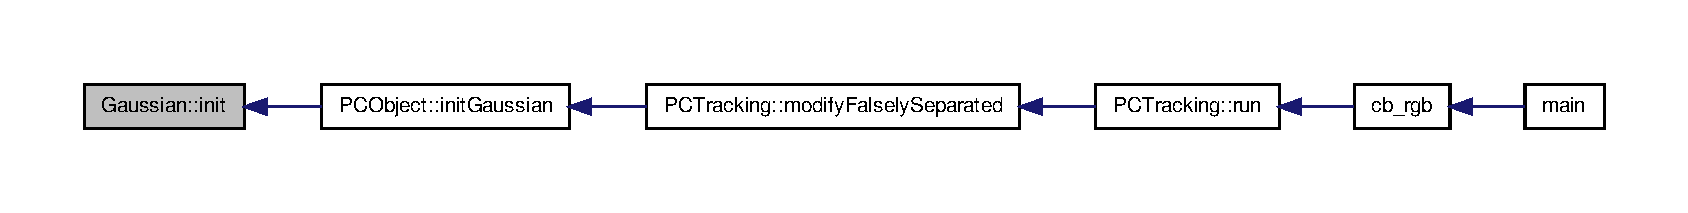
\includegraphics[width=350pt]{class_gaussian_adf54537aeb68ac96fc3dc0bd42224216_icgraph}
\end{center}
\end{figure}


\hypertarget{class_gaussian_a8e447c419d940ee28016c56bf1c3fa6c}{\index{\-Gaussian@{\-Gaussian}!init\-Prediction@{init\-Prediction}}
\index{init\-Prediction@{init\-Prediction}!Gaussian@{\-Gaussian}}
\subsubsection[{init\-Prediction}]{\setlength{\rightskip}{0pt plus 5cm}void {\bf \-Gaussian\-::init\-Prediction} (
\begin{DoxyParamCaption}
{}
\end{DoxyParamCaption}
)}}\label{class_gaussian_a8e447c419d940ee28016c56bf1c3fa6c}


\-Here is the caller graph for this function\-:
\nopagebreak
\begin{figure}[H]
\begin{center}
\leavevmode
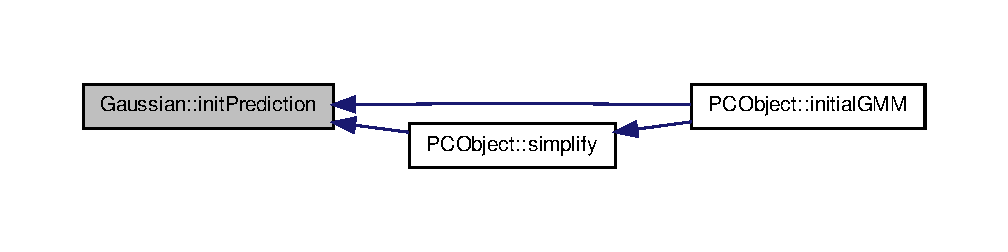
\includegraphics[width=350pt]{class_gaussian_a8e447c419d940ee28016c56bf1c3fa6c_icgraph}
\end{center}
\end{figure}


\hypertarget{class_gaussian_a7c8e5d982d6c20e36c68d3d042f0e9c5}{\index{\-Gaussian@{\-Gaussian}!quaternion2rotation@{quaternion2rotation}}
\index{quaternion2rotation@{quaternion2rotation}!Gaussian@{\-Gaussian}}
\subsubsection[{quaternion2rotation}]{\setlength{\rightskip}{0pt plus 5cm}void {\bf \-Gaussian\-::quaternion2rotation} (
\begin{DoxyParamCaption}
\item[{vnl\-\_\-vector$<$ double $>$}]{q, }
\item[{vnl\-\_\-matrix$<$ double $>$ \&}]{\-R, }
\item[{vnl\-\_\-matrix$<$ double $>$ \&}]{g1, }
\item[{vnl\-\_\-matrix$<$ double $>$ \&}]{g2, }
\item[{vnl\-\_\-matrix$<$ double $>$ \&}]{g3, }
\item[{vnl\-\_\-matrix$<$ double $>$ \&}]{g4}
\end{DoxyParamCaption}
)\hspace{0.3cm}{\ttfamily  \mbox{[}static\mbox{]}}}}\label{class_gaussian_a7c8e5d982d6c20e36c68d3d042f0e9c5}


\-Here is the caller graph for this function\-:
\nopagebreak
\begin{figure}[H]
\begin{center}
\leavevmode
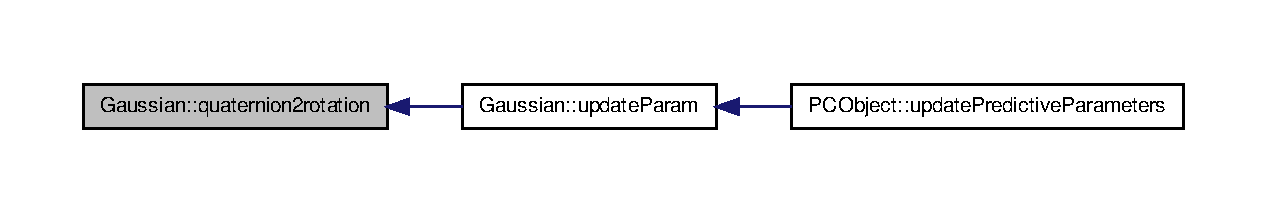
\includegraphics[width=350pt]{class_gaussian_a7c8e5d982d6c20e36c68d3d042f0e9c5_icgraph}
\end{center}
\end{figure}


\hypertarget{class_gaussian_aa3bbdc57cb1715d5e97f28e277649ced}{\index{\-Gaussian@{\-Gaussian}!quaternion2rotation@{quaternion2rotation}}
\index{quaternion2rotation@{quaternion2rotation}!Gaussian@{\-Gaussian}}
\subsubsection[{quaternion2rotation}]{\setlength{\rightskip}{0pt plus 5cm}void {\bf \-Gaussian\-::quaternion2rotation} (
\begin{DoxyParamCaption}
\item[{vnl\-\_\-vector$<$ double $>$}]{q, }
\item[{vnl\-\_\-matrix$<$ double $>$ \&}]{\-R}
\end{DoxyParamCaption}
)\hspace{0.3cm}{\ttfamily  \mbox{[}static\mbox{]}}}}\label{class_gaussian_aa3bbdc57cb1715d5e97f28e277649ced}
\hypertarget{class_gaussian_a6d157086ac90e226afd46887fa43c5a8}{\index{\-Gaussian@{\-Gaussian}!update\-Param@{update\-Param}}
\index{update\-Param@{update\-Param}!Gaussian@{\-Gaussian}}
\subsubsection[{update\-Param}]{\setlength{\rightskip}{0pt plus 5cm}void {\bf \-Gaussian\-::update\-Param} (
\begin{DoxyParamCaption}
\item[{vnl\-\_\-vector$<$ double $>$}]{new\-Param}
\end{DoxyParamCaption}
)}}\label{class_gaussian_a6d157086ac90e226afd46887fa43c5a8}


\-Here is the call graph for this function\-:
\nopagebreak
\begin{figure}[H]
\begin{center}
\leavevmode
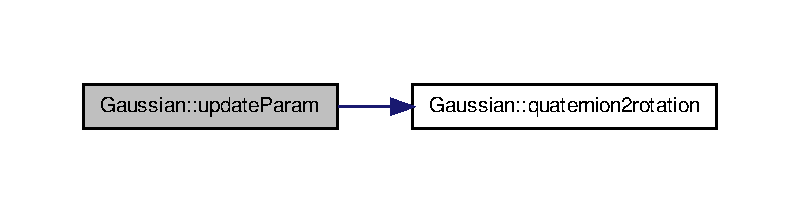
\includegraphics[width=350pt]{class_gaussian_a6d157086ac90e226afd46887fa43c5a8_cgraph}
\end{center}
\end{figure}




\-Here is the caller graph for this function\-:
\nopagebreak
\begin{figure}[H]
\begin{center}
\leavevmode
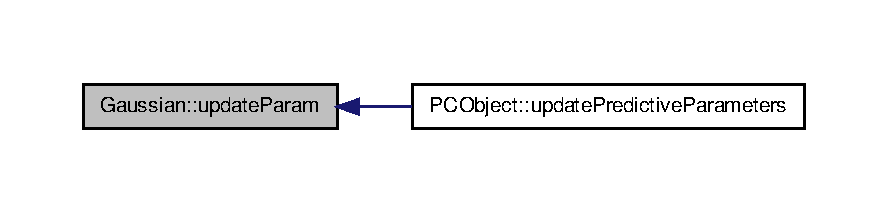
\includegraphics[width=350pt]{class_gaussian_a6d157086ac90e226afd46887fa43c5a8_icgraph}
\end{center}
\end{figure}




\subsection{\-Member \-Data \-Documentation}
\hypertarget{class_gaussian_a5c2ddadca218776ecc2d47ee7dfb2244}{\index{\-Gaussian@{\-Gaussian}!cov\-\_\-determinant@{cov\-\_\-determinant}}
\index{cov\-\_\-determinant@{cov\-\_\-determinant}!Gaussian@{\-Gaussian}}
\subsubsection[{cov\-\_\-determinant}]{\setlength{\rightskip}{0pt plus 5cm}double {\bf \-Gaussian\-::cov\-\_\-determinant}}}\label{class_gaussian_a5c2ddadca218776ecc2d47ee7dfb2244}
\hypertarget{class_gaussian_af2381be5187cf33c49d1c4575382b588}{\index{\-Gaussian@{\-Gaussian}!cov\-\_\-inverse@{cov\-\_\-inverse}}
\index{cov\-\_\-inverse@{cov\-\_\-inverse}!Gaussian@{\-Gaussian}}
\subsubsection[{cov\-\_\-inverse}]{\setlength{\rightskip}{0pt plus 5cm}\-Eigen\-::\-Matrix\-Xd {\bf \-Gaussian\-::cov\-\_\-inverse}}}\label{class_gaussian_af2381be5187cf33c49d1c4575382b588}
\hypertarget{class_gaussian_a62f08da00092ff4db7e0b864a2a68466}{\index{\-Gaussian@{\-Gaussian}!covariance@{covariance}}
\index{covariance@{covariance}!Gaussian@{\-Gaussian}}
\subsubsection[{covariance}]{\setlength{\rightskip}{0pt plus 5cm}\-Eigen\-::\-Matrix\-Xd {\bf \-Gaussian\-::covariance}}}\label{class_gaussian_a62f08da00092ff4db7e0b864a2a68466}
\hypertarget{class_gaussian_ac8cca436c08c5c880bc1d7b6f9fae31d}{\index{\-Gaussian@{\-Gaussian}!dim@{dim}}
\index{dim@{dim}!Gaussian@{\-Gaussian}}
\subsubsection[{dim}]{\setlength{\rightskip}{0pt plus 5cm}int {\bf \-Gaussian\-::dim}}}\label{class_gaussian_ac8cca436c08c5c880bc1d7b6f9fae31d}
\hypertarget{class_gaussian_a040f0491de0917c6f9ad79ae7e68c02c}{\index{\-Gaussian@{\-Gaussian}!eigenvalues@{eigenvalues}}
\index{eigenvalues@{eigenvalues}!Gaussian@{\-Gaussian}}
\subsubsection[{eigenvalues}]{\setlength{\rightskip}{0pt plus 5cm}\-Eigen\-::\-Vector3d {\bf \-Gaussian\-::eigenvalues}}}\label{class_gaussian_a040f0491de0917c6f9ad79ae7e68c02c}
\hypertarget{class_gaussian_a430bc29a81c8a70d1ef6d9442bf7ba6f}{\index{\-Gaussian@{\-Gaussian}!eigenvectors@{eigenvectors}}
\index{eigenvectors@{eigenvectors}!Gaussian@{\-Gaussian}}
\subsubsection[{eigenvectors}]{\setlength{\rightskip}{0pt plus 5cm}\-Eigen\-::\-Matrix3d {\bf \-Gaussian\-::eigenvectors}}}\label{class_gaussian_a430bc29a81c8a70d1ef6d9442bf7ba6f}
\hypertarget{class_gaussian_acf67c5d6f25b4c13bfcfd72db9ab544f}{\index{\-Gaussian@{\-Gaussian}!is\-Empty@{is\-Empty}}
\index{is\-Empty@{is\-Empty}!Gaussian@{\-Gaussian}}
\subsubsection[{is\-Empty}]{\setlength{\rightskip}{0pt plus 5cm}bool {\bf \-Gaussian\-::is\-Empty}}}\label{class_gaussian_acf67c5d6f25b4c13bfcfd72db9ab544f}
\hypertarget{class_gaussian_a2462f56c5ce1b88275ab4c59b99739a4}{\index{\-Gaussian@{\-Gaussian}!mean@{mean}}
\index{mean@{mean}!Gaussian@{\-Gaussian}}
\subsubsection[{mean}]{\setlength{\rightskip}{0pt plus 5cm}\-Eigen\-::\-Vector\-Xd {\bf \-Gaussian\-::mean}}}\label{class_gaussian_a2462f56c5ce1b88275ab4c59b99739a4}
\hypertarget{class_gaussian_a736f42df8823b1397eff83858e7864d1}{\index{\-Gaussian@{\-Gaussian}!n\-Point@{n\-Point}}
\index{n\-Point@{n\-Point}!Gaussian@{\-Gaussian}}
\subsubsection[{n\-Point}]{\setlength{\rightskip}{0pt plus 5cm}int {\bf \-Gaussian\-::n\-Point}}}\label{class_gaussian_a736f42df8823b1397eff83858e7864d1}
\hypertarget{class_gaussian_afadc9984777174ca00506af635c9db1a}{\index{\-Gaussian@{\-Gaussian}!predictive\-\_\-covariance@{predictive\-\_\-covariance}}
\index{predictive\-\_\-covariance@{predictive\-\_\-covariance}!Gaussian@{\-Gaussian}}
\subsubsection[{predictive\-\_\-covariance}]{\setlength{\rightskip}{0pt plus 5cm}\-Eigen\-::\-Matrix\-Xd {\bf \-Gaussian\-::predictive\-\_\-covariance}}}\label{class_gaussian_afadc9984777174ca00506af635c9db1a}
\hypertarget{class_gaussian_af57af53a8c6d0006cc8a6a7658198eb0}{\index{\-Gaussian@{\-Gaussian}!predictive\-\_\-mean@{predictive\-\_\-mean}}
\index{predictive\-\_\-mean@{predictive\-\_\-mean}!Gaussian@{\-Gaussian}}
\subsubsection[{predictive\-\_\-mean}]{\setlength{\rightskip}{0pt plus 5cm}\-Eigen\-::\-Vector\-Xd {\bf \-Gaussian\-::predictive\-\_\-mean}}}\label{class_gaussian_af57af53a8c6d0006cc8a6a7658198eb0}
\hypertarget{class_gaussian_a859907145de3080604d20cc1105cd1e5}{\index{\-Gaussian@{\-Gaussian}!rotation@{rotation}}
\index{rotation@{rotation}!Gaussian@{\-Gaussian}}
\subsubsection[{rotation}]{\setlength{\rightskip}{0pt plus 5cm}vnl\-\_\-matrix$<$double$>$ {\bf \-Gaussian\-::rotation}}}\label{class_gaussian_a859907145de3080604d20cc1105cd1e5}
\hypertarget{class_gaussian_a2469316effaaf6d03566d534fefa64fc}{\index{\-Gaussian@{\-Gaussian}!translation@{translation}}
\index{translation@{translation}!Gaussian@{\-Gaussian}}
\subsubsection[{translation}]{\setlength{\rightskip}{0pt plus 5cm}vnl\-\_\-matrix$<$double$>$ {\bf \-Gaussian\-::translation}}}\label{class_gaussian_a2469316effaaf6d03566d534fefa64fc}
\hypertarget{class_gaussian_a09ad4d04a27b2e6be4945719da025927}{\index{\-Gaussian@{\-Gaussian}!velocity@{velocity}}
\index{velocity@{velocity}!Gaussian@{\-Gaussian}}
\subsubsection[{velocity}]{\setlength{\rightskip}{0pt plus 5cm}\-Eigen\-::\-Vector3d {\bf \-Gaussian\-::velocity}}}\label{class_gaussian_a09ad4d04a27b2e6be4945719da025927}
\hypertarget{class_gaussian_ae6192dadf70b84fa41dcf4498b5aaf52}{\index{\-Gaussian@{\-Gaussian}!weight@{weight}}
\index{weight@{weight}!Gaussian@{\-Gaussian}}
\subsubsection[{weight}]{\setlength{\rightskip}{0pt plus 5cm}double {\bf \-Gaussian\-::weight}}}\label{class_gaussian_ae6192dadf70b84fa41dcf4498b5aaf52}


\-The documentation for this class was generated from the following files\-:\begin{DoxyCompactItemize}
\item 
/home/koosy/koosywork/pmot\-\_\-realtime/pmot\-\_\-realtime/src/\hyperlink{gaussian_8h}{gaussian.\-h}\item 
/home/koosy/koosywork/pmot\-\_\-realtime/pmot\-\_\-realtime/src/\hyperlink{gaussian_8cpp}{gaussian.\-cpp}\end{DoxyCompactItemize}

\hypertarget{class_gaussian_track_container}{\section{\-Gaussian\-Track\-Container \-Class \-Reference}
\label{class_gaussian_track_container}\index{\-Gaussian\-Track\-Container@{\-Gaussian\-Track\-Container}}
}


{\ttfamily \#include $<$gaussiantrackcontainer.\-h$>$}



\-Inheritance diagram for \-Gaussian\-Track\-Container\-:
\nopagebreak
\begin{figure}[H]
\begin{center}
\leavevmode
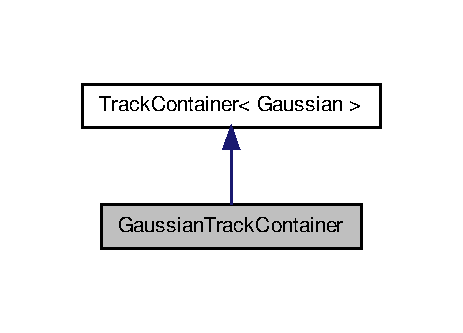
\includegraphics[width=222pt]{class_gaussian_track_container__inherit__graph}
\end{center}
\end{figure}


\-Collaboration diagram for \-Gaussian\-Track\-Container\-:
\nopagebreak
\begin{figure}[H]
\begin{center}
\leavevmode
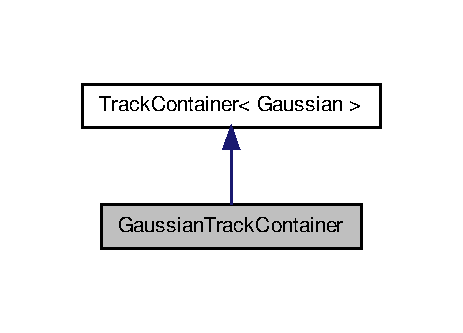
\includegraphics[width=222pt]{class_gaussian_track_container__coll__graph}
\end{center}
\end{figure}
\subsection*{\-Public \-Member \-Functions}
\begin{DoxyCompactItemize}
\item 
\hyperlink{class_gaussian_track_container_ae4ea80c9acddbd13d1122f187c5c2e2b}{\-Gaussian\-Track\-Container} (int \-\_\-max\-Frame=1000)
\end{DoxyCompactItemize}


\subsection{\-Constructor \& \-Destructor \-Documentation}
\hypertarget{class_gaussian_track_container_ae4ea80c9acddbd13d1122f187c5c2e2b}{\index{\-Gaussian\-Track\-Container@{\-Gaussian\-Track\-Container}!\-Gaussian\-Track\-Container@{\-Gaussian\-Track\-Container}}
\index{\-Gaussian\-Track\-Container@{\-Gaussian\-Track\-Container}!GaussianTrackContainer@{\-Gaussian\-Track\-Container}}
\subsubsection[{\-Gaussian\-Track\-Container}]{\setlength{\rightskip}{0pt plus 5cm}{\bf \-Gaussian\-Track\-Container\-::\-Gaussian\-Track\-Container} (
\begin{DoxyParamCaption}
\item[{int}]{\-\_\-max\-Frame = {\ttfamily 1000}}
\end{DoxyParamCaption}
)}}\label{class_gaussian_track_container_ae4ea80c9acddbd13d1122f187c5c2e2b}


\-The documentation for this class was generated from the following files\-:\begin{DoxyCompactItemize}
\item 
/home/koosy/koosywork/pmot\-\_\-realtime/pmot\-\_\-realtime/src/\hyperlink{gaussiantrackcontainer_8h}{gaussiantrackcontainer.\-h}\item 
/home/koosy/koosywork/pmot\-\_\-realtime/pmot\-\_\-realtime/src/\hyperlink{gaussiantrackcontainer_8cpp}{gaussiantrackcontainer.\-cpp}\end{DoxyCompactItemize}

\hypertarget{class_gaus_vcsh}{\section{\-Gaus\-Vcsh \-Class \-Reference}
\label{class_gaus_vcsh}\index{\-Gaus\-Vcsh@{\-Gaus\-Vcsh}}
}


{\ttfamily \#include $<$csfeature.\-h$>$}



\-Collaboration diagram for \-Gaus\-Vcsh\-:
\nopagebreak
\begin{figure}[H]
\begin{center}
\leavevmode
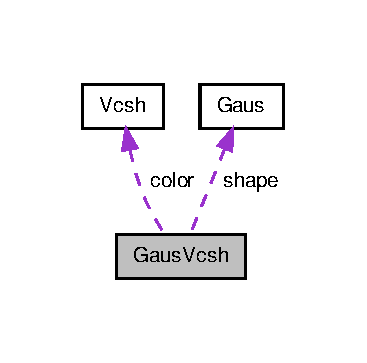
\includegraphics[width=176pt]{class_gaus_vcsh__coll__graph}
\end{center}
\end{figure}
\subsection*{\-Public \-Member \-Functions}
\begin{DoxyCompactItemize}
\item 
void \hyperlink{class_gaus_vcsh_aae7b05d4ce56c36fd9a7dc8f155a1e2a}{generate} (float gridsize)
\item 
float \hyperlink{class_gaus_vcsh_aafe812bc24a5904b6a195986ab21ef28}{get\-Dist} (\hyperlink{class_gaus_vcsh}{\-Gaus\-Vcsh} other)
\end{DoxyCompactItemize}
\subsection*{\-Public \-Attributes}
\begin{DoxyCompactItemize}
\item 
\hyperlink{class_gaus}{\-Gaus} \hyperlink{class_gaus_vcsh_ad12e2a864c80579b2c4b6cb7b32743ca}{shape}
\item 
\hyperlink{class_vcsh}{\-Vcsh} \hyperlink{class_gaus_vcsh_adcb434fb6a698a468cb6c87ef456c360}{color}
\item 
std\-::vector$<$ \hyperlink{common_8h_af63aa02ad22799ec1b392e97942874b5}{\-Point\-T} $>$ \hyperlink{class_gaus_vcsh_a4fb32a8c7eb116b2e56788e2b128fb25}{points}
\end{DoxyCompactItemize}


\subsection{\-Member \-Function \-Documentation}
\hypertarget{class_gaus_vcsh_aae7b05d4ce56c36fd9a7dc8f155a1e2a}{\index{\-Gaus\-Vcsh@{\-Gaus\-Vcsh}!generate@{generate}}
\index{generate@{generate}!GausVcsh@{\-Gaus\-Vcsh}}
\subsubsection[{generate}]{\setlength{\rightskip}{0pt plus 5cm}void {\bf \-Gaus\-Vcsh\-::generate} (
\begin{DoxyParamCaption}
\item[{float}]{gridsize}
\end{DoxyParamCaption}
)}}\label{class_gaus_vcsh_aae7b05d4ce56c36fd9a7dc8f155a1e2a}


\-Here is the call graph for this function\-:
\nopagebreak
\begin{figure}[H]
\begin{center}
\leavevmode
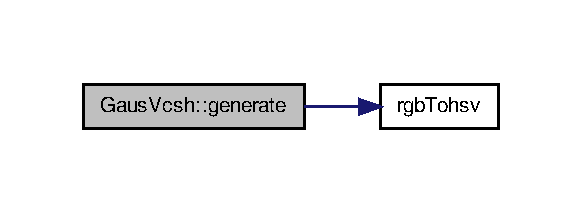
\includegraphics[width=280pt]{class_gaus_vcsh_aae7b05d4ce56c36fd9a7dc8f155a1e2a_cgraph}
\end{center}
\end{figure}


\hypertarget{class_gaus_vcsh_aafe812bc24a5904b6a195986ab21ef28}{\index{\-Gaus\-Vcsh@{\-Gaus\-Vcsh}!get\-Dist@{get\-Dist}}
\index{get\-Dist@{get\-Dist}!GausVcsh@{\-Gaus\-Vcsh}}
\subsubsection[{get\-Dist}]{\setlength{\rightskip}{0pt plus 5cm}float {\bf \-Gaus\-Vcsh\-::get\-Dist} (
\begin{DoxyParamCaption}
\item[{{\bf \-Gaus\-Vcsh}}]{other}
\end{DoxyParamCaption}
)}}\label{class_gaus_vcsh_aafe812bc24a5904b6a195986ab21ef28}


\subsection{\-Member \-Data \-Documentation}
\hypertarget{class_gaus_vcsh_adcb434fb6a698a468cb6c87ef456c360}{\index{\-Gaus\-Vcsh@{\-Gaus\-Vcsh}!color@{color}}
\index{color@{color}!GausVcsh@{\-Gaus\-Vcsh}}
\subsubsection[{color}]{\setlength{\rightskip}{0pt plus 5cm}{\bf \-Vcsh} {\bf \-Gaus\-Vcsh\-::color}}}\label{class_gaus_vcsh_adcb434fb6a698a468cb6c87ef456c360}
\hypertarget{class_gaus_vcsh_a4fb32a8c7eb116b2e56788e2b128fb25}{\index{\-Gaus\-Vcsh@{\-Gaus\-Vcsh}!points@{points}}
\index{points@{points}!GausVcsh@{\-Gaus\-Vcsh}}
\subsubsection[{points}]{\setlength{\rightskip}{0pt plus 5cm}std\-::vector$<${\bf \-Point\-T}$>$ {\bf \-Gaus\-Vcsh\-::points}}}\label{class_gaus_vcsh_a4fb32a8c7eb116b2e56788e2b128fb25}
\hypertarget{class_gaus_vcsh_ad12e2a864c80579b2c4b6cb7b32743ca}{\index{\-Gaus\-Vcsh@{\-Gaus\-Vcsh}!shape@{shape}}
\index{shape@{shape}!GausVcsh@{\-Gaus\-Vcsh}}
\subsubsection[{shape}]{\setlength{\rightskip}{0pt plus 5cm}{\bf \-Gaus} {\bf \-Gaus\-Vcsh\-::shape}}}\label{class_gaus_vcsh_ad12e2a864c80579b2c4b6cb7b32743ca}


\-The documentation for this class was generated from the following files\-:\begin{DoxyCompactItemize}
\item 
/home/koosy/koosywork/pmot\-\_\-realtime/pmot\-\_\-realtime/src/\hyperlink{csfeature_8h}{csfeature.\-h}\item 
/home/koosy/koosywork/pmot\-\_\-realtime/pmot\-\_\-realtime/src/\hyperlink{csfeature_8cpp}{csfeature.\-cpp}\end{DoxyCompactItemize}

\hypertarget{class_i_m_f_t}{\section{\-I\-M\-F\-T$<$ \-Object $>$ \-Class \-Template \-Reference}
\label{class_i_m_f_t}\index{\-I\-M\-F\-T$<$ Object $>$@{\-I\-M\-F\-T$<$ Object $>$}}
}


{\ttfamily \#include $<$imft.\-h$>$}



\-Collaboration diagram for \-I\-M\-F\-T$<$ \-Object $>$\-:
\nopagebreak
\begin{figure}[H]
\begin{center}
\leavevmode
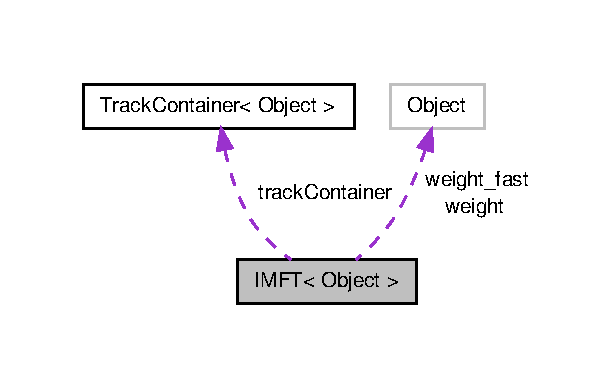
\includegraphics[width=295pt]{class_i_m_f_t__coll__graph}
\end{center}
\end{figure}
\subsection*{\-Public \-Types}
\begin{DoxyCompactItemize}
\item 
typedef \hyperlink{class_track_container}{\-Track\-Container}$<$ \-Object $>$ \hyperlink{class_i_m_f_t_a8aad0b1bd309bfb92abb74ce45e549a9}{\-Track\-Container\-T}
\item 
typedef \hyperlink{class_track}{\-Track}$<$ \-Object $>$ \hyperlink{class_i_m_f_t_a37f74f73fc6d19920930474c5522e242}{\-Track\-T}
\item 
typedef \hyperlink{struct_track_1_1_frame}{\-Track\-T\-::\-Frame} \hyperlink{class_i_m_f_t_ab9da2d474c63076c3a194d343fc20169}{\-Ptr}
\item 
typedef vector$<$ \hyperlink{class_i_m_f_t_ab9da2d474c63076c3a194d343fc20169}{\-Ptr} $>$ \hyperlink{class_i_m_f_t_a47e5af5b3e023928bd7ddc6ddbf6044c}{\-Vec\-Ptr}
\item 
typedef \hyperlink{struct_track_1_1_v}{\-Track\-T\-::\-V} \hyperlink{class_i_m_f_t_ad22184fa80718f8e5087d8cec78a6323}{\-V}
\item 
typedef vector$<$ \hyperlink{class_i_m_f_t_a37f74f73fc6d19920930474c5522e242}{\-Track\-T} $>$ \hyperlink{class_i_m_f_t_a55e4fd327687c579749d3ca13e0f621e}{\-Vec\-Track}
\item 
typedef double($\ast$ \hyperlink{class_i_m_f_t_ae7436174afe28b7a25237c97b2b9f416}{func\-Weight} )(\-Object \&o1, \-Object \&o2)
\item 
typedef \-Object $\ast$ \hyperlink{class_i_m_f_t_a9f291b28e2caab20361d790d02774dfe}{\-Object\-Ptr}
\item 
typedef vector$<$ \-Object $\ast$ $>$ \hyperlink{class_i_m_f_t_a03dc658b57ff8debb2b6869be37c0d67}{\-Vec\-Object\-Ptr}
\end{DoxyCompactItemize}
\subsection*{\-Public \-Member \-Functions}
\begin{DoxyCompactItemize}
\item 
\hyperlink{class_i_m_f_t_adfcb341712779443d1f22168b807f90c}{\-I\-M\-F\-T} (int \-\_\-window\-\_\-short=10, int \-\_\-window\-\_\-long=20, int \-\_\-max\-I\-D=100, \hyperlink{class_i_m_f_t_ae7436174afe28b7a25237c97b2b9f416}{func\-Weight} \-\_\-weight=0, \hyperlink{class_i_m_f_t_ae7436174afe28b7a25237c97b2b9f416}{func\-Weight} \-\_\-weight\-\_\-fast=0)
\item 
\hyperlink{class_i_m_f_t_ac669bb45bbc9b72c4dea37097c66d661}{$\sim$\-I\-M\-F\-T} ()
\item 
void \hyperlink{class_i_m_f_t_ad47b95cc538fd0b52e8f0cf276dda86c}{set\-Frame} (vector$<$ \-Object $\ast$ $>$ objects, int stamp)
\item 
void \hyperlink{class_i_m_f_t_acb040ebe38d14012375f000a9f4df0b9}{confirm\-D\-Graph} ()
\item 
void \hyperlink{class_i_m_f_t_a8a0e5ca756776227e239a67e186938f7}{extension} ()
\item 
void \hyperlink{class_i_m_f_t_a1c4e1853b1dcaf86e50a1ced421af6ad}{matching} ()
\item 
void \hyperlink{class_i_m_f_t_a7b9ee3a95b6586bb08152d872289e042}{update\-Tracks} ()
\item 
\hyperlink{class_i_m_f_t_a8aad0b1bd309bfb92abb74ce45e549a9}{\-Track\-Container\-T} $\ast$ \hyperlink{class_i_m_f_t_a0dcd3c2c2747177fc4ea4f1bb73bae7b}{extract\-Tracks} ()
\item 
\hyperlink{class_i_m_f_t_a03dc658b57ff8debb2b6869be37c0d67}{\-Vec\-Object\-Ptr} \hyperlink{class_i_m_f_t_ad9803bbc0eef9c8680377052793c029c}{get\-Unmatched\-Objects} ()
\item 
\hyperlink{class_i_m_f_t_a03dc658b57ff8debb2b6869be37c0d67}{\-Vec\-Object\-Ptr} \hyperlink{class_i_m_f_t_afe0b6e7d641820f7c8d3bd8b2ed42ec7}{get\-Terminal\-Nodes} ()
\item 
\hyperlink{class_i_m_f_t_a03dc658b57ff8debb2b6869be37c0d67}{\-Vec\-Object\-Ptr} \hyperlink{class_i_m_f_t_a51b02ea25f4830c396608e41ad2dda4d}{get\-Terminal\-Nodes\-Last\-Frame} ()
\item 
\hyperlink{class_i_m_f_t_a03dc658b57ff8debb2b6869be37c0d67}{\-Vec\-Object\-Ptr} \hyperlink{class_i_m_f_t_a981a25796eaf59f23c8819001ab9ee9e}{get\-Unmatched\-Tracks} ()
\item 
void \hyperlink{class_i_m_f_t_a0fc1cd8b04d246ef33f84f5b0c40ac6a}{get\-Maximum\-Matched\-Track} (\hyperlink{class_i_m_f_t_a9f291b28e2caab20361d790d02774dfe}{\-Object\-Ptr} object, \hyperlink{class_i_m_f_t_a9f291b28e2caab20361d790d02774dfe}{\-Object\-Ptr} \&max\-Track, double \&w\-Hypothesis, \hyperlink{class_i_m_f_t_a9f291b28e2caab20361d790d02774dfe}{\-Object\-Ptr} \&object\-Origin, double \&w\-Origin)
\item 
void \hyperlink{class_i_m_f_t_a4fa24de7283cacd230302a47bf9aa424}{get\-Maximum\-Matched\-Object} (\hyperlink{class_i_m_f_t_a9f291b28e2caab20361d790d02774dfe}{\-Object\-Ptr} track\-Unmatched, \hyperlink{class_i_m_f_t_a9f291b28e2caab20361d790d02774dfe}{\-Object\-Ptr} \&max\-Object, double \&w\-Hypothesis, \hyperlink{class_i_m_f_t_a9f291b28e2caab20361d790d02774dfe}{\-Object\-Ptr} \&track\-Origin, double \&w\-Origin)
\item 
bool \hyperlink{class_i_m_f_t_afc129366861aecc3edf1c98fef27f5bf}{delete\-Last\-Frame} ()
\end{DoxyCompactItemize}
\subsection*{\-Public \-Attributes}
\begin{DoxyCompactItemize}
\item 
\hyperlink{class_i_m_f_t_ae7436174afe28b7a25237c97b2b9f416}{func\-Weight} \hyperlink{class_i_m_f_t_ac25f8710b5133e975dd7be2e9909f0bd}{weight}
\item 
\hyperlink{class_i_m_f_t_ae7436174afe28b7a25237c97b2b9f416}{func\-Weight} \hyperlink{class_i_m_f_t_a9431008dbf21f96477c515c41b77014f}{weight\-\_\-fast}
\item 
\hyperlink{class_i_m_f_t_a8aad0b1bd309bfb92abb74ce45e549a9}{\-Track\-Container\-T} $\ast$ \hyperlink{class_i_m_f_t_a2b7798fca0fac14339c47ce517778560}{track\-Container}
\item 
int \hyperlink{class_i_m_f_t_aa470d46dee0f624f461d8854939cd6c5}{cnt}
\item 
int \hyperlink{class_i_m_f_t_ad2198a7256eb82e0c5ad0362abc5290a}{window\-\_\-short}
\item 
int \hyperlink{class_i_m_f_t_a90e2ffc6a77b2b27035c8dfc6cbb8378}{window\-\_\-long}
\item 
int \hyperlink{class_i_m_f_t_abb14e14b1278312f13d5e45bb0bedd47}{max\-I\-D}
\item 
bool \hyperlink{class_i_m_f_t_af10936c7ab5ea0b0d18e928365c6ff3d}{m\-\_\-is\-Debug}
\item 
\-List\-Graph \hyperlink{class_i_m_f_t_a03887af2ae2372fcbecc2525176bbef8}{m\-\_\-g}
\item 
\-List\-Graph\-::\-Node\-Map$<$ \hyperlink{class_i_m_f_t_ad22184fa80718f8e5087d8cec78a6323}{\-V} $>$ $\ast$ \hyperlink{class_i_m_f_t_a456c4e69b77870a87f0d6a86b33ce668}{m\-\_\-g\-Node\-Map}
\item 
\-List\-Graph\-::\-Edge\-Map$<$ double $>$ $\ast$ \hyperlink{class_i_m_f_t_a9629eb1da0d08013c87c4e679c176c6b}{m\-\_\-g\-Edge\-Map}
\item 
double \hyperlink{class_i_m_f_t_a157d578f41bcddf7355c9d0fc16c0f6e}{m\-\_\-max\-Weight}
\item 
vector$<$ int $>$ \hyperlink{class_i_m_f_t_a29f477074ca9cb6760c58c7312a0e2c6}{m\-\_\-vec\-Old\-Edge}
\item 
double \hyperlink{class_i_m_f_t_ac759c0713923c5a609ec3e90b942f606}{m\-\_\-wsum}
\item 
int \hyperlink{class_i_m_f_t_afd30e2f7af8158e10d95c1e55a05e17d}{m\-\_\-current\-T}
\item 
int \hyperlink{class_i_m_f_t_a1fbf73806f8ad8cc86261808f7c4ec09}{m\-\_\-new\-Track\-I\-D}
\end{DoxyCompactItemize}
\subsection*{\-Private \-Member \-Functions}
\begin{DoxyCompactItemize}
\item 
void \hyperlink{class_i_m_f_t_a4afe4b84cad4d3915d888d3da46496f1}{moving\-Window} ()
\item 
void \hyperlink{class_i_m_f_t_aba2080902249baf70c7788e97cf7f6a7}{add\-To\-D\-Graph} (\hyperlink{class_i_m_f_t_a47e5af5b3e023928bd7ddc6ddbf6044c}{\-Vec\-Ptr} ptrs)
\item 
void \hyperlink{class_i_m_f_t_a7f73ff3d638dd056ce848e50f18ec3a9}{two\-Frame\-Corresponding} (vector$<$ \-List\-Graph\-::\-Node $>$ vec\-U\-Frame, vector$<$ \-List\-Graph\-::\-Node $>$ vec\-V\-Frame)
\end{DoxyCompactItemize}
\subsubsection*{template$<$class \-Object$>$ class I\-M\-F\-T$<$ Object $>$}



\subsection{\-Member \-Typedef \-Documentation}
\hypertarget{class_i_m_f_t_ae7436174afe28b7a25237c97b2b9f416}{\index{\-I\-M\-F\-T@{\-I\-M\-F\-T}!func\-Weight@{func\-Weight}}
\index{func\-Weight@{func\-Weight}!IMFT@{\-I\-M\-F\-T}}
\subsubsection[{func\-Weight}]{\setlength{\rightskip}{0pt plus 5cm}template$<$class \-Object$>$ typedef double($\ast$ {\bf \-I\-M\-F\-T}$<$ \-Object $>$\-::{\bf func\-Weight})(\-Object \&o1, \-Object \&o2)}}\label{class_i_m_f_t_ae7436174afe28b7a25237c97b2b9f416}
\hypertarget{class_i_m_f_t_a9f291b28e2caab20361d790d02774dfe}{\index{\-I\-M\-F\-T@{\-I\-M\-F\-T}!\-Object\-Ptr@{\-Object\-Ptr}}
\index{\-Object\-Ptr@{\-Object\-Ptr}!IMFT@{\-I\-M\-F\-T}}
\subsubsection[{\-Object\-Ptr}]{\setlength{\rightskip}{0pt plus 5cm}template$<$class \-Object$>$ typedef \-Object$\ast$ {\bf \-I\-M\-F\-T}$<$ \-Object $>$\-::{\bf \-Object\-Ptr}}}\label{class_i_m_f_t_a9f291b28e2caab20361d790d02774dfe}
\hypertarget{class_i_m_f_t_ab9da2d474c63076c3a194d343fc20169}{\index{\-I\-M\-F\-T@{\-I\-M\-F\-T}!\-Ptr@{\-Ptr}}
\index{\-Ptr@{\-Ptr}!IMFT@{\-I\-M\-F\-T}}
\subsubsection[{\-Ptr}]{\setlength{\rightskip}{0pt plus 5cm}template$<$class \-Object$>$ typedef {\bf \-Track\-T\-::\-Frame} {\bf \-I\-M\-F\-T}$<$ \-Object $>$\-::{\bf \-Ptr}}}\label{class_i_m_f_t_ab9da2d474c63076c3a194d343fc20169}
\hypertarget{class_i_m_f_t_a8aad0b1bd309bfb92abb74ce45e549a9}{\index{\-I\-M\-F\-T@{\-I\-M\-F\-T}!\-Track\-Container\-T@{\-Track\-Container\-T}}
\index{\-Track\-Container\-T@{\-Track\-Container\-T}!IMFT@{\-I\-M\-F\-T}}
\subsubsection[{\-Track\-Container\-T}]{\setlength{\rightskip}{0pt plus 5cm}template$<$class \-Object$>$ typedef {\bf \-Track\-Container}$<$\-Object$>$ {\bf \-I\-M\-F\-T}$<$ \-Object $>$\-::{\bf \-Track\-Container\-T}}}\label{class_i_m_f_t_a8aad0b1bd309bfb92abb74ce45e549a9}
\hypertarget{class_i_m_f_t_a37f74f73fc6d19920930474c5522e242}{\index{\-I\-M\-F\-T@{\-I\-M\-F\-T}!\-Track\-T@{\-Track\-T}}
\index{\-Track\-T@{\-Track\-T}!IMFT@{\-I\-M\-F\-T}}
\subsubsection[{\-Track\-T}]{\setlength{\rightskip}{0pt plus 5cm}template$<$class \-Object$>$ typedef {\bf \-Track}$<$\-Object$>$ {\bf \-I\-M\-F\-T}$<$ \-Object $>$\-::{\bf \-Track\-T}}}\label{class_i_m_f_t_a37f74f73fc6d19920930474c5522e242}
\hypertarget{class_i_m_f_t_ad22184fa80718f8e5087d8cec78a6323}{\index{\-I\-M\-F\-T@{\-I\-M\-F\-T}!\-V@{\-V}}
\index{\-V@{\-V}!IMFT@{\-I\-M\-F\-T}}
\subsubsection[{\-V}]{\setlength{\rightskip}{0pt plus 5cm}template$<$class \-Object$>$ typedef {\bf \-Track\-T\-::\-V} {\bf \-I\-M\-F\-T}$<$ \-Object $>$\-::{\bf \-V}}}\label{class_i_m_f_t_ad22184fa80718f8e5087d8cec78a6323}
\hypertarget{class_i_m_f_t_a03dc658b57ff8debb2b6869be37c0d67}{\index{\-I\-M\-F\-T@{\-I\-M\-F\-T}!\-Vec\-Object\-Ptr@{\-Vec\-Object\-Ptr}}
\index{\-Vec\-Object\-Ptr@{\-Vec\-Object\-Ptr}!IMFT@{\-I\-M\-F\-T}}
\subsubsection[{\-Vec\-Object\-Ptr}]{\setlength{\rightskip}{0pt plus 5cm}template$<$class \-Object$>$ typedef vector$<$\-Object$\ast$$>$ {\bf \-I\-M\-F\-T}$<$ \-Object $>$\-::{\bf \-Vec\-Object\-Ptr}}}\label{class_i_m_f_t_a03dc658b57ff8debb2b6869be37c0d67}
\hypertarget{class_i_m_f_t_a47e5af5b3e023928bd7ddc6ddbf6044c}{\index{\-I\-M\-F\-T@{\-I\-M\-F\-T}!\-Vec\-Ptr@{\-Vec\-Ptr}}
\index{\-Vec\-Ptr@{\-Vec\-Ptr}!IMFT@{\-I\-M\-F\-T}}
\subsubsection[{\-Vec\-Ptr}]{\setlength{\rightskip}{0pt plus 5cm}template$<$class \-Object$>$ typedef vector$<${\bf \-Ptr}$>$ {\bf \-I\-M\-F\-T}$<$ \-Object $>$\-::{\bf \-Vec\-Ptr}}}\label{class_i_m_f_t_a47e5af5b3e023928bd7ddc6ddbf6044c}
\hypertarget{class_i_m_f_t_a55e4fd327687c579749d3ca13e0f621e}{\index{\-I\-M\-F\-T@{\-I\-M\-F\-T}!\-Vec\-Track@{\-Vec\-Track}}
\index{\-Vec\-Track@{\-Vec\-Track}!IMFT@{\-I\-M\-F\-T}}
\subsubsection[{\-Vec\-Track}]{\setlength{\rightskip}{0pt plus 5cm}template$<$class \-Object$>$ typedef vector$<${\bf \-Track\-T}$>$ {\bf \-I\-M\-F\-T}$<$ \-Object $>$\-::{\bf \-Vec\-Track}}}\label{class_i_m_f_t_a55e4fd327687c579749d3ca13e0f621e}


\subsection{\-Constructor \& \-Destructor \-Documentation}
\hypertarget{class_i_m_f_t_adfcb341712779443d1f22168b807f90c}{\index{\-I\-M\-F\-T@{\-I\-M\-F\-T}!\-I\-M\-F\-T@{\-I\-M\-F\-T}}
\index{\-I\-M\-F\-T@{\-I\-M\-F\-T}!IMFT@{\-I\-M\-F\-T}}
\subsubsection[{\-I\-M\-F\-T}]{\setlength{\rightskip}{0pt plus 5cm}template$<$class Object $>$ {\bf \-I\-M\-F\-T}$<$ \-Object $>$\-::{\bf \-I\-M\-F\-T} (
\begin{DoxyParamCaption}
\item[{int}]{\-\_\-window\-\_\-short = {\ttfamily 10}, }
\item[{int}]{\-\_\-window\-\_\-long = {\ttfamily 20}, }
\item[{int}]{\-\_\-max\-I\-D = {\ttfamily 100}, }
\item[{{\bf func\-Weight}}]{\-\_\-weight = {\ttfamily 0}, }
\item[{{\bf func\-Weight}}]{\-\_\-weight\-\_\-fast = {\ttfamily 0}}
\end{DoxyParamCaption}
)}}\label{class_i_m_f_t_adfcb341712779443d1f22168b807f90c}
\hypertarget{class_i_m_f_t_ac669bb45bbc9b72c4dea37097c66d661}{\index{\-I\-M\-F\-T@{\-I\-M\-F\-T}!$\sim$\-I\-M\-F\-T@{$\sim$\-I\-M\-F\-T}}
\index{$\sim$\-I\-M\-F\-T@{$\sim$\-I\-M\-F\-T}!IMFT@{\-I\-M\-F\-T}}
\subsubsection[{$\sim$\-I\-M\-F\-T}]{\setlength{\rightskip}{0pt plus 5cm}template$<$class Object $>$ {\bf \-I\-M\-F\-T}$<$ \-Object $>$\-::$\sim${\bf \-I\-M\-F\-T} (
\begin{DoxyParamCaption}
{}
\end{DoxyParamCaption}
)}}\label{class_i_m_f_t_ac669bb45bbc9b72c4dea37097c66d661}


\subsection{\-Member \-Function \-Documentation}
\hypertarget{class_i_m_f_t_aba2080902249baf70c7788e97cf7f6a7}{\index{\-I\-M\-F\-T@{\-I\-M\-F\-T}!add\-To\-D\-Graph@{add\-To\-D\-Graph}}
\index{add\-To\-D\-Graph@{add\-To\-D\-Graph}!IMFT@{\-I\-M\-F\-T}}
\subsubsection[{add\-To\-D\-Graph}]{\setlength{\rightskip}{0pt plus 5cm}template$<$class Object $>$ void {\bf \-I\-M\-F\-T}$<$ \-Object $>$\-::{\bf add\-To\-D\-Graph} (
\begin{DoxyParamCaption}
\item[{{\bf \-Vec\-Ptr}}]{ptrs}
\end{DoxyParamCaption}
)\hspace{0.3cm}{\ttfamily  \mbox{[}private\mbox{]}}}}\label{class_i_m_f_t_aba2080902249baf70c7788e97cf7f6a7}
\hypertarget{class_i_m_f_t_acb040ebe38d14012375f000a9f4df0b9}{\index{\-I\-M\-F\-T@{\-I\-M\-F\-T}!confirm\-D\-Graph@{confirm\-D\-Graph}}
\index{confirm\-D\-Graph@{confirm\-D\-Graph}!IMFT@{\-I\-M\-F\-T}}
\subsubsection[{confirm\-D\-Graph}]{\setlength{\rightskip}{0pt plus 5cm}template$<$class Object $>$ void {\bf \-I\-M\-F\-T}$<$ \-Object $>$\-::{\bf confirm\-D\-Graph} (
\begin{DoxyParamCaption}
{}
\end{DoxyParamCaption}
)}}\label{class_i_m_f_t_acb040ebe38d14012375f000a9f4df0b9}
\hypertarget{class_i_m_f_t_afc129366861aecc3edf1c98fef27f5bf}{\index{\-I\-M\-F\-T@{\-I\-M\-F\-T}!delete\-Last\-Frame@{delete\-Last\-Frame}}
\index{delete\-Last\-Frame@{delete\-Last\-Frame}!IMFT@{\-I\-M\-F\-T}}
\subsubsection[{delete\-Last\-Frame}]{\setlength{\rightskip}{0pt plus 5cm}template$<$class Object $>$ bool {\bf \-I\-M\-F\-T}$<$ \-Object $>$\-::{\bf delete\-Last\-Frame} (
\begin{DoxyParamCaption}
{}
\end{DoxyParamCaption}
)}}\label{class_i_m_f_t_afc129366861aecc3edf1c98fef27f5bf}
\hypertarget{class_i_m_f_t_a8a0e5ca756776227e239a67e186938f7}{\index{\-I\-M\-F\-T@{\-I\-M\-F\-T}!extension@{extension}}
\index{extension@{extension}!IMFT@{\-I\-M\-F\-T}}
\subsubsection[{extension}]{\setlength{\rightskip}{0pt plus 5cm}template$<$class Object $>$ void {\bf \-I\-M\-F\-T}$<$ \-Object $>$\-::{\bf extension} (
\begin{DoxyParamCaption}
{}
\end{DoxyParamCaption}
)}}\label{class_i_m_f_t_a8a0e5ca756776227e239a67e186938f7}
\hypertarget{class_i_m_f_t_a0dcd3c2c2747177fc4ea4f1bb73bae7b}{\index{\-I\-M\-F\-T@{\-I\-M\-F\-T}!extract\-Tracks@{extract\-Tracks}}
\index{extract\-Tracks@{extract\-Tracks}!IMFT@{\-I\-M\-F\-T}}
\subsubsection[{extract\-Tracks}]{\setlength{\rightskip}{0pt plus 5cm}template$<$class Object $>$ {\bf \-I\-M\-F\-T}$<$ \-Object $>$\-::{\bf \-Track\-Container\-T} $\ast$ {\bf \-I\-M\-F\-T}$<$ \-Object $>$\-::{\bf extract\-Tracks} (
\begin{DoxyParamCaption}
{}
\end{DoxyParamCaption}
)}}\label{class_i_m_f_t_a0dcd3c2c2747177fc4ea4f1bb73bae7b}


\-Here is the caller graph for this function\-:
\nopagebreak
\begin{figure}[H]
\begin{center}
\leavevmode
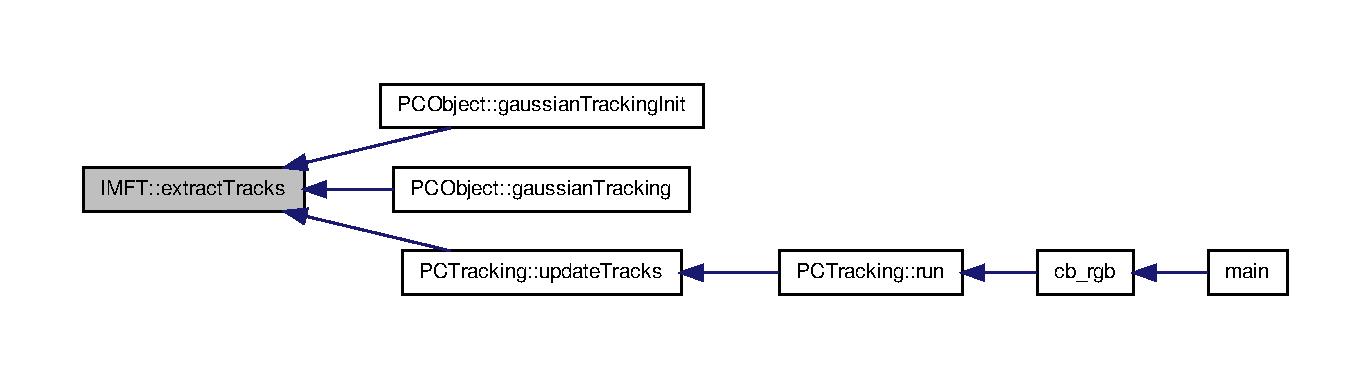
\includegraphics[width=350pt]{class_i_m_f_t_a0dcd3c2c2747177fc4ea4f1bb73bae7b_icgraph}
\end{center}
\end{figure}


\hypertarget{class_i_m_f_t_a4fa24de7283cacd230302a47bf9aa424}{\index{\-I\-M\-F\-T@{\-I\-M\-F\-T}!get\-Maximum\-Matched\-Object@{get\-Maximum\-Matched\-Object}}
\index{get\-Maximum\-Matched\-Object@{get\-Maximum\-Matched\-Object}!IMFT@{\-I\-M\-F\-T}}
\subsubsection[{get\-Maximum\-Matched\-Object}]{\setlength{\rightskip}{0pt plus 5cm}template$<$class Object $>$ void {\bf \-I\-M\-F\-T}$<$ \-Object $>$\-::{\bf get\-Maximum\-Matched\-Object} (
\begin{DoxyParamCaption}
\item[{{\bf \-Object\-Ptr}}]{track\-Unmatched, }
\item[{{\bf \-Object\-Ptr} \&}]{max\-Object, }
\item[{double \&}]{w\-Hypothesis, }
\item[{{\bf \-Object\-Ptr} \&}]{track\-Origin, }
\item[{double \&}]{w\-Origin}
\end{DoxyParamCaption}
)}}\label{class_i_m_f_t_a4fa24de7283cacd230302a47bf9aa424}
\hypertarget{class_i_m_f_t_a0fc1cd8b04d246ef33f84f5b0c40ac6a}{\index{\-I\-M\-F\-T@{\-I\-M\-F\-T}!get\-Maximum\-Matched\-Track@{get\-Maximum\-Matched\-Track}}
\index{get\-Maximum\-Matched\-Track@{get\-Maximum\-Matched\-Track}!IMFT@{\-I\-M\-F\-T}}
\subsubsection[{get\-Maximum\-Matched\-Track}]{\setlength{\rightskip}{0pt plus 5cm}template$<$class Object $>$ void {\bf \-I\-M\-F\-T}$<$ \-Object $>$\-::{\bf get\-Maximum\-Matched\-Track} (
\begin{DoxyParamCaption}
\item[{{\bf \-Object\-Ptr}}]{object, }
\item[{{\bf \-Object\-Ptr} \&}]{max\-Track, }
\item[{double \&}]{w\-Hypothesis, }
\item[{{\bf \-Object\-Ptr} \&}]{object\-Origin, }
\item[{double \&}]{w\-Origin}
\end{DoxyParamCaption}
)}}\label{class_i_m_f_t_a0fc1cd8b04d246ef33f84f5b0c40ac6a}
\hypertarget{class_i_m_f_t_afe0b6e7d641820f7c8d3bd8b2ed42ec7}{\index{\-I\-M\-F\-T@{\-I\-M\-F\-T}!get\-Terminal\-Nodes@{get\-Terminal\-Nodes}}
\index{get\-Terminal\-Nodes@{get\-Terminal\-Nodes}!IMFT@{\-I\-M\-F\-T}}
\subsubsection[{get\-Terminal\-Nodes}]{\setlength{\rightskip}{0pt plus 5cm}template$<$class Object $>$ {\bf \-I\-M\-F\-T}$<$ \-Object $>$\-::{\bf \-Vec\-Object\-Ptr} {\bf \-I\-M\-F\-T}$<$ \-Object $>$\-::{\bf get\-Terminal\-Nodes} (
\begin{DoxyParamCaption}
{}
\end{DoxyParamCaption}
)}}\label{class_i_m_f_t_afe0b6e7d641820f7c8d3bd8b2ed42ec7}
\hypertarget{class_i_m_f_t_a51b02ea25f4830c396608e41ad2dda4d}{\index{\-I\-M\-F\-T@{\-I\-M\-F\-T}!get\-Terminal\-Nodes\-Last\-Frame@{get\-Terminal\-Nodes\-Last\-Frame}}
\index{get\-Terminal\-Nodes\-Last\-Frame@{get\-Terminal\-Nodes\-Last\-Frame}!IMFT@{\-I\-M\-F\-T}}
\subsubsection[{get\-Terminal\-Nodes\-Last\-Frame}]{\setlength{\rightskip}{0pt plus 5cm}template$<$class Object $>$ {\bf \-I\-M\-F\-T}$<$ \-Object $>$\-::{\bf \-Vec\-Object\-Ptr} {\bf \-I\-M\-F\-T}$<$ \-Object $>$\-::{\bf get\-Terminal\-Nodes\-Last\-Frame} (
\begin{DoxyParamCaption}
{}
\end{DoxyParamCaption}
)}}\label{class_i_m_f_t_a51b02ea25f4830c396608e41ad2dda4d}
\hypertarget{class_i_m_f_t_ad9803bbc0eef9c8680377052793c029c}{\index{\-I\-M\-F\-T@{\-I\-M\-F\-T}!get\-Unmatched\-Objects@{get\-Unmatched\-Objects}}
\index{get\-Unmatched\-Objects@{get\-Unmatched\-Objects}!IMFT@{\-I\-M\-F\-T}}
\subsubsection[{get\-Unmatched\-Objects}]{\setlength{\rightskip}{0pt plus 5cm}template$<$class Object $>$ {\bf \-I\-M\-F\-T}$<$ \-Object $>$\-::{\bf \-Vec\-Object\-Ptr} {\bf \-I\-M\-F\-T}$<$ \-Object $>$\-::{\bf get\-Unmatched\-Objects} (
\begin{DoxyParamCaption}
{}
\end{DoxyParamCaption}
)}}\label{class_i_m_f_t_ad9803bbc0eef9c8680377052793c029c}
\hypertarget{class_i_m_f_t_a981a25796eaf59f23c8819001ab9ee9e}{\index{\-I\-M\-F\-T@{\-I\-M\-F\-T}!get\-Unmatched\-Tracks@{get\-Unmatched\-Tracks}}
\index{get\-Unmatched\-Tracks@{get\-Unmatched\-Tracks}!IMFT@{\-I\-M\-F\-T}}
\subsubsection[{get\-Unmatched\-Tracks}]{\setlength{\rightskip}{0pt plus 5cm}template$<$class Object $>$ {\bf \-I\-M\-F\-T}$<$ \-Object $>$\-::{\bf \-Vec\-Object\-Ptr} {\bf \-I\-M\-F\-T}$<$ \-Object $>$\-::{\bf get\-Unmatched\-Tracks} (
\begin{DoxyParamCaption}
{}
\end{DoxyParamCaption}
)}}\label{class_i_m_f_t_a981a25796eaf59f23c8819001ab9ee9e}
\hypertarget{class_i_m_f_t_a1c4e1853b1dcaf86e50a1ced421af6ad}{\index{\-I\-M\-F\-T@{\-I\-M\-F\-T}!matching@{matching}}
\index{matching@{matching}!IMFT@{\-I\-M\-F\-T}}
\subsubsection[{matching}]{\setlength{\rightskip}{0pt plus 5cm}template$<$class Object $>$ void {\bf \-I\-M\-F\-T}$<$ \-Object $>$\-::{\bf matching} (
\begin{DoxyParamCaption}
{}
\end{DoxyParamCaption}
)}}\label{class_i_m_f_t_a1c4e1853b1dcaf86e50a1ced421af6ad}


\-Here is the caller graph for this function\-:
\nopagebreak
\begin{figure}[H]
\begin{center}
\leavevmode
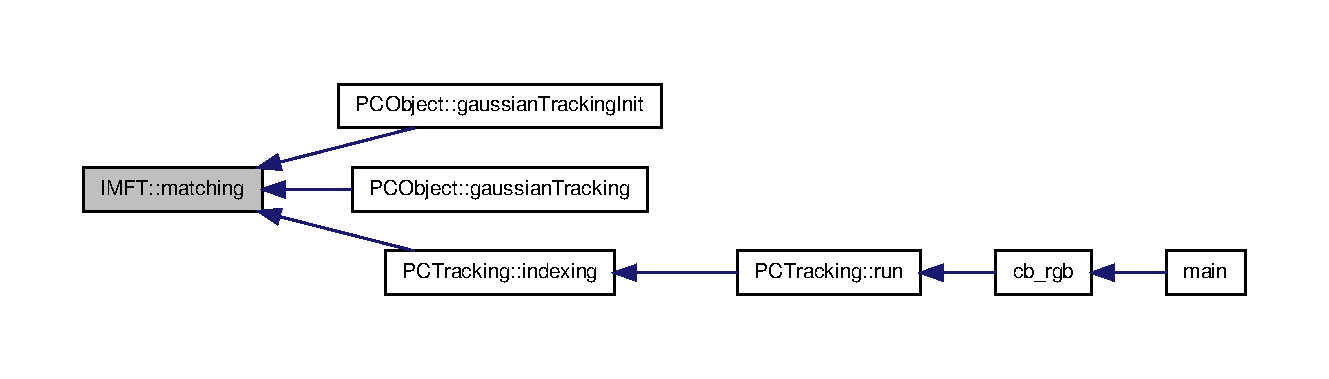
\includegraphics[width=350pt]{class_i_m_f_t_a1c4e1853b1dcaf86e50a1ced421af6ad_icgraph}
\end{center}
\end{figure}


\hypertarget{class_i_m_f_t_a4afe4b84cad4d3915d888d3da46496f1}{\index{\-I\-M\-F\-T@{\-I\-M\-F\-T}!moving\-Window@{moving\-Window}}
\index{moving\-Window@{moving\-Window}!IMFT@{\-I\-M\-F\-T}}
\subsubsection[{moving\-Window}]{\setlength{\rightskip}{0pt plus 5cm}template$<$class Object $>$ void {\bf \-I\-M\-F\-T}$<$ \-Object $>$\-::{\bf moving\-Window} (
\begin{DoxyParamCaption}
{}
\end{DoxyParamCaption}
)\hspace{0.3cm}{\ttfamily  \mbox{[}private\mbox{]}}}}\label{class_i_m_f_t_a4afe4b84cad4d3915d888d3da46496f1}
\hypertarget{class_i_m_f_t_ad47b95cc538fd0b52e8f0cf276dda86c}{\index{\-I\-M\-F\-T@{\-I\-M\-F\-T}!set\-Frame@{set\-Frame}}
\index{set\-Frame@{set\-Frame}!IMFT@{\-I\-M\-F\-T}}
\subsubsection[{set\-Frame}]{\setlength{\rightskip}{0pt plus 5cm}template$<$class \-Object$>$ void {\bf \-I\-M\-F\-T}$<$ \-Object $>$\-::{\bf set\-Frame} (
\begin{DoxyParamCaption}
\item[{vector$<$ \-Object $\ast$ $>$}]{objects, }
\item[{int}]{stamp}
\end{DoxyParamCaption}
)}}\label{class_i_m_f_t_ad47b95cc538fd0b52e8f0cf276dda86c}


\-Here is the caller graph for this function\-:
\nopagebreak
\begin{figure}[H]
\begin{center}
\leavevmode
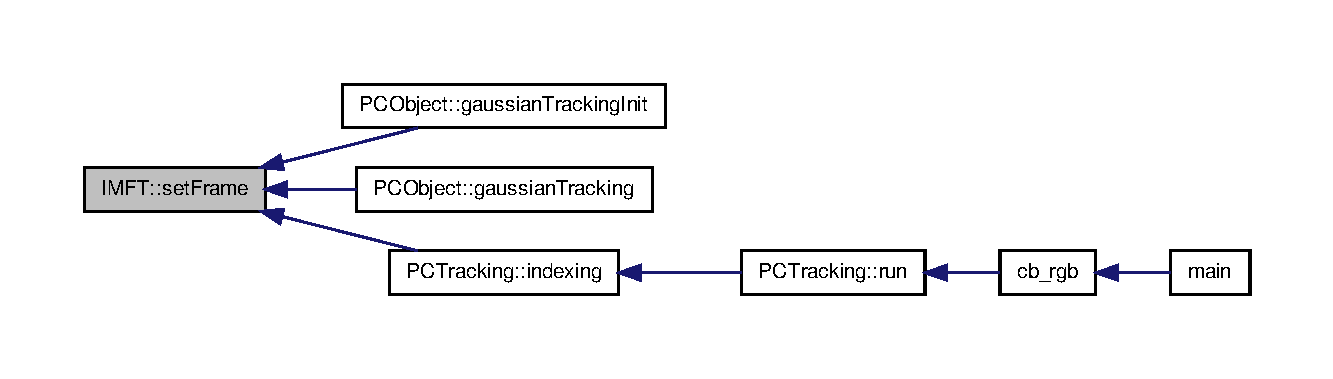
\includegraphics[width=350pt]{class_i_m_f_t_ad47b95cc538fd0b52e8f0cf276dda86c_icgraph}
\end{center}
\end{figure}


\hypertarget{class_i_m_f_t_a7f73ff3d638dd056ce848e50f18ec3a9}{\index{\-I\-M\-F\-T@{\-I\-M\-F\-T}!two\-Frame\-Corresponding@{two\-Frame\-Corresponding}}
\index{two\-Frame\-Corresponding@{two\-Frame\-Corresponding}!IMFT@{\-I\-M\-F\-T}}
\subsubsection[{two\-Frame\-Corresponding}]{\setlength{\rightskip}{0pt plus 5cm}template$<$typename Object $>$ void {\bf \-I\-M\-F\-T}$<$ \-Object $>$\-::{\bf two\-Frame\-Corresponding} (
\begin{DoxyParamCaption}
\item[{vector$<$ \-List\-Graph\-::\-Node $>$}]{vec\-U\-Frame, }
\item[{vector$<$ \-List\-Graph\-::\-Node $>$}]{vec\-V\-Frame}
\end{DoxyParamCaption}
)\hspace{0.3cm}{\ttfamily  \mbox{[}private\mbox{]}}}}\label{class_i_m_f_t_a7f73ff3d638dd056ce848e50f18ec3a9}
\hypertarget{class_i_m_f_t_a7b9ee3a95b6586bb08152d872289e042}{\index{\-I\-M\-F\-T@{\-I\-M\-F\-T}!update\-Tracks@{update\-Tracks}}
\index{update\-Tracks@{update\-Tracks}!IMFT@{\-I\-M\-F\-T}}
\subsubsection[{update\-Tracks}]{\setlength{\rightskip}{0pt plus 5cm}template$<$class Object $>$ void {\bf \-I\-M\-F\-T}$<$ \-Object $>$\-::{\bf update\-Tracks} (
\begin{DoxyParamCaption}
{}
\end{DoxyParamCaption}
)}}\label{class_i_m_f_t_a7b9ee3a95b6586bb08152d872289e042}


\-Here is the caller graph for this function\-:
\nopagebreak
\begin{figure}[H]
\begin{center}
\leavevmode
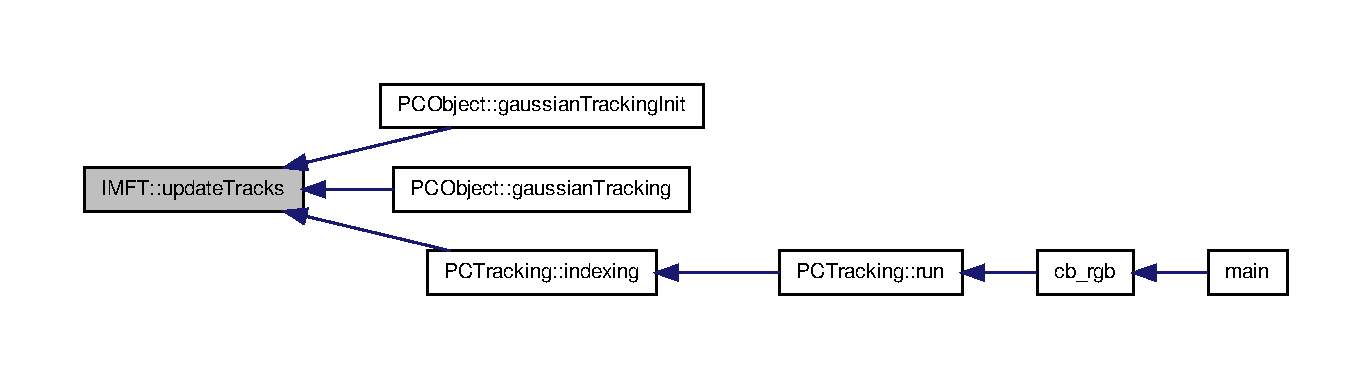
\includegraphics[width=350pt]{class_i_m_f_t_a7b9ee3a95b6586bb08152d872289e042_icgraph}
\end{center}
\end{figure}




\subsection{\-Member \-Data \-Documentation}
\hypertarget{class_i_m_f_t_aa470d46dee0f624f461d8854939cd6c5}{\index{\-I\-M\-F\-T@{\-I\-M\-F\-T}!cnt@{cnt}}
\index{cnt@{cnt}!IMFT@{\-I\-M\-F\-T}}
\subsubsection[{cnt}]{\setlength{\rightskip}{0pt plus 5cm}template$<$class \-Object$>$ int {\bf \-I\-M\-F\-T}$<$ \-Object $>$\-::{\bf cnt}}}\label{class_i_m_f_t_aa470d46dee0f624f461d8854939cd6c5}
\hypertarget{class_i_m_f_t_afd30e2f7af8158e10d95c1e55a05e17d}{\index{\-I\-M\-F\-T@{\-I\-M\-F\-T}!m\-\_\-current\-T@{m\-\_\-current\-T}}
\index{m\-\_\-current\-T@{m\-\_\-current\-T}!IMFT@{\-I\-M\-F\-T}}
\subsubsection[{m\-\_\-current\-T}]{\setlength{\rightskip}{0pt plus 5cm}template$<$class \-Object$>$ int {\bf \-I\-M\-F\-T}$<$ \-Object $>$\-::{\bf m\-\_\-current\-T}}}\label{class_i_m_f_t_afd30e2f7af8158e10d95c1e55a05e17d}
\hypertarget{class_i_m_f_t_a03887af2ae2372fcbecc2525176bbef8}{\index{\-I\-M\-F\-T@{\-I\-M\-F\-T}!m\-\_\-g@{m\-\_\-g}}
\index{m\-\_\-g@{m\-\_\-g}!IMFT@{\-I\-M\-F\-T}}
\subsubsection[{m\-\_\-g}]{\setlength{\rightskip}{0pt plus 5cm}template$<$class \-Object$>$ \-List\-Graph {\bf \-I\-M\-F\-T}$<$ \-Object $>$\-::{\bf m\-\_\-g}}}\label{class_i_m_f_t_a03887af2ae2372fcbecc2525176bbef8}
\hypertarget{class_i_m_f_t_a9629eb1da0d08013c87c4e679c176c6b}{\index{\-I\-M\-F\-T@{\-I\-M\-F\-T}!m\-\_\-g\-Edge\-Map@{m\-\_\-g\-Edge\-Map}}
\index{m\-\_\-g\-Edge\-Map@{m\-\_\-g\-Edge\-Map}!IMFT@{\-I\-M\-F\-T}}
\subsubsection[{m\-\_\-g\-Edge\-Map}]{\setlength{\rightskip}{0pt plus 5cm}template$<$class \-Object$>$ \-List\-Graph\-::\-Edge\-Map$<$double$>$$\ast$ {\bf \-I\-M\-F\-T}$<$ \-Object $>$\-::{\bf m\-\_\-g\-Edge\-Map}}}\label{class_i_m_f_t_a9629eb1da0d08013c87c4e679c176c6b}
\hypertarget{class_i_m_f_t_a456c4e69b77870a87f0d6a86b33ce668}{\index{\-I\-M\-F\-T@{\-I\-M\-F\-T}!m\-\_\-g\-Node\-Map@{m\-\_\-g\-Node\-Map}}
\index{m\-\_\-g\-Node\-Map@{m\-\_\-g\-Node\-Map}!IMFT@{\-I\-M\-F\-T}}
\subsubsection[{m\-\_\-g\-Node\-Map}]{\setlength{\rightskip}{0pt plus 5cm}template$<$class \-Object$>$ \-List\-Graph\-::\-Node\-Map$<${\bf \-V}$>$$\ast$ {\bf \-I\-M\-F\-T}$<$ \-Object $>$\-::{\bf m\-\_\-g\-Node\-Map}}}\label{class_i_m_f_t_a456c4e69b77870a87f0d6a86b33ce668}
\hypertarget{class_i_m_f_t_af10936c7ab5ea0b0d18e928365c6ff3d}{\index{\-I\-M\-F\-T@{\-I\-M\-F\-T}!m\-\_\-is\-Debug@{m\-\_\-is\-Debug}}
\index{m\-\_\-is\-Debug@{m\-\_\-is\-Debug}!IMFT@{\-I\-M\-F\-T}}
\subsubsection[{m\-\_\-is\-Debug}]{\setlength{\rightskip}{0pt plus 5cm}template$<$class \-Object$>$ bool {\bf \-I\-M\-F\-T}$<$ \-Object $>$\-::{\bf m\-\_\-is\-Debug}}}\label{class_i_m_f_t_af10936c7ab5ea0b0d18e928365c6ff3d}
\hypertarget{class_i_m_f_t_a157d578f41bcddf7355c9d0fc16c0f6e}{\index{\-I\-M\-F\-T@{\-I\-M\-F\-T}!m\-\_\-max\-Weight@{m\-\_\-max\-Weight}}
\index{m\-\_\-max\-Weight@{m\-\_\-max\-Weight}!IMFT@{\-I\-M\-F\-T}}
\subsubsection[{m\-\_\-max\-Weight}]{\setlength{\rightskip}{0pt plus 5cm}template$<$class \-Object$>$ double {\bf \-I\-M\-F\-T}$<$ \-Object $>$\-::{\bf m\-\_\-max\-Weight}}}\label{class_i_m_f_t_a157d578f41bcddf7355c9d0fc16c0f6e}
\hypertarget{class_i_m_f_t_a1fbf73806f8ad8cc86261808f7c4ec09}{\index{\-I\-M\-F\-T@{\-I\-M\-F\-T}!m\-\_\-new\-Track\-I\-D@{m\-\_\-new\-Track\-I\-D}}
\index{m\-\_\-new\-Track\-I\-D@{m\-\_\-new\-Track\-I\-D}!IMFT@{\-I\-M\-F\-T}}
\subsubsection[{m\-\_\-new\-Track\-I\-D}]{\setlength{\rightskip}{0pt plus 5cm}template$<$class \-Object$>$ int {\bf \-I\-M\-F\-T}$<$ \-Object $>$\-::{\bf m\-\_\-new\-Track\-I\-D}}}\label{class_i_m_f_t_a1fbf73806f8ad8cc86261808f7c4ec09}
\hypertarget{class_i_m_f_t_a29f477074ca9cb6760c58c7312a0e2c6}{\index{\-I\-M\-F\-T@{\-I\-M\-F\-T}!m\-\_\-vec\-Old\-Edge@{m\-\_\-vec\-Old\-Edge}}
\index{m\-\_\-vec\-Old\-Edge@{m\-\_\-vec\-Old\-Edge}!IMFT@{\-I\-M\-F\-T}}
\subsubsection[{m\-\_\-vec\-Old\-Edge}]{\setlength{\rightskip}{0pt plus 5cm}template$<$class \-Object$>$ vector$<$int$>$ {\bf \-I\-M\-F\-T}$<$ \-Object $>$\-::{\bf m\-\_\-vec\-Old\-Edge}}}\label{class_i_m_f_t_a29f477074ca9cb6760c58c7312a0e2c6}
\hypertarget{class_i_m_f_t_ac759c0713923c5a609ec3e90b942f606}{\index{\-I\-M\-F\-T@{\-I\-M\-F\-T}!m\-\_\-wsum@{m\-\_\-wsum}}
\index{m\-\_\-wsum@{m\-\_\-wsum}!IMFT@{\-I\-M\-F\-T}}
\subsubsection[{m\-\_\-wsum}]{\setlength{\rightskip}{0pt plus 5cm}template$<$class \-Object$>$ double {\bf \-I\-M\-F\-T}$<$ \-Object $>$\-::{\bf m\-\_\-wsum}}}\label{class_i_m_f_t_ac759c0713923c5a609ec3e90b942f606}
\hypertarget{class_i_m_f_t_abb14e14b1278312f13d5e45bb0bedd47}{\index{\-I\-M\-F\-T@{\-I\-M\-F\-T}!max\-I\-D@{max\-I\-D}}
\index{max\-I\-D@{max\-I\-D}!IMFT@{\-I\-M\-F\-T}}
\subsubsection[{max\-I\-D}]{\setlength{\rightskip}{0pt plus 5cm}template$<$class \-Object$>$ int {\bf \-I\-M\-F\-T}$<$ \-Object $>$\-::{\bf max\-I\-D}}}\label{class_i_m_f_t_abb14e14b1278312f13d5e45bb0bedd47}
\hypertarget{class_i_m_f_t_a2b7798fca0fac14339c47ce517778560}{\index{\-I\-M\-F\-T@{\-I\-M\-F\-T}!track\-Container@{track\-Container}}
\index{track\-Container@{track\-Container}!IMFT@{\-I\-M\-F\-T}}
\subsubsection[{track\-Container}]{\setlength{\rightskip}{0pt plus 5cm}template$<$class \-Object$>$ {\bf \-Track\-Container\-T}$\ast$ {\bf \-I\-M\-F\-T}$<$ \-Object $>$\-::{\bf track\-Container}}}\label{class_i_m_f_t_a2b7798fca0fac14339c47ce517778560}
\hypertarget{class_i_m_f_t_ac25f8710b5133e975dd7be2e9909f0bd}{\index{\-I\-M\-F\-T@{\-I\-M\-F\-T}!weight@{weight}}
\index{weight@{weight}!IMFT@{\-I\-M\-F\-T}}
\subsubsection[{weight}]{\setlength{\rightskip}{0pt plus 5cm}template$<$class \-Object$>$ {\bf func\-Weight} {\bf \-I\-M\-F\-T}$<$ \-Object $>$\-::{\bf weight}}}\label{class_i_m_f_t_ac25f8710b5133e975dd7be2e9909f0bd}
\hypertarget{class_i_m_f_t_a9431008dbf21f96477c515c41b77014f}{\index{\-I\-M\-F\-T@{\-I\-M\-F\-T}!weight\-\_\-fast@{weight\-\_\-fast}}
\index{weight\-\_\-fast@{weight\-\_\-fast}!IMFT@{\-I\-M\-F\-T}}
\subsubsection[{weight\-\_\-fast}]{\setlength{\rightskip}{0pt plus 5cm}template$<$class \-Object$>$ {\bf func\-Weight} {\bf \-I\-M\-F\-T}$<$ \-Object $>$\-::{\bf weight\-\_\-fast}}}\label{class_i_m_f_t_a9431008dbf21f96477c515c41b77014f}
\hypertarget{class_i_m_f_t_a90e2ffc6a77b2b27035c8dfc6cbb8378}{\index{\-I\-M\-F\-T@{\-I\-M\-F\-T}!window\-\_\-long@{window\-\_\-long}}
\index{window\-\_\-long@{window\-\_\-long}!IMFT@{\-I\-M\-F\-T}}
\subsubsection[{window\-\_\-long}]{\setlength{\rightskip}{0pt plus 5cm}template$<$class \-Object$>$ int {\bf \-I\-M\-F\-T}$<$ \-Object $>$\-::{\bf window\-\_\-long}}}\label{class_i_m_f_t_a90e2ffc6a77b2b27035c8dfc6cbb8378}
\hypertarget{class_i_m_f_t_ad2198a7256eb82e0c5ad0362abc5290a}{\index{\-I\-M\-F\-T@{\-I\-M\-F\-T}!window\-\_\-short@{window\-\_\-short}}
\index{window\-\_\-short@{window\-\_\-short}!IMFT@{\-I\-M\-F\-T}}
\subsubsection[{window\-\_\-short}]{\setlength{\rightskip}{0pt plus 5cm}template$<$class \-Object$>$ int {\bf \-I\-M\-F\-T}$<$ \-Object $>$\-::{\bf window\-\_\-short}}}\label{class_i_m_f_t_ad2198a7256eb82e0c5ad0362abc5290a}


\-The documentation for this class was generated from the following files\-:\begin{DoxyCompactItemize}
\item 
/home/koosy/koosywork/pmot\-\_\-realtime/pmot\-\_\-realtime/src/\hyperlink{imft_8h}{imft.\-h}\item 
/home/koosy/koosywork/pmot\-\_\-realtime/pmot\-\_\-realtime/src/\hyperlink{imft_8hpp}{imft.\-hpp}\end{DoxyCompactItemize}

\hypertarget{struct_track_1_1_node}{\section{\-Track$<$ \-Object $>$\-:\-:\-Node \-Struct \-Reference}
\label{struct_track_1_1_node}\index{\-Track$<$ Object $>$\-::\-Node@{\-Track$<$ Object $>$\-::\-Node}}
}


{\ttfamily \#include $<$track.\-h$>$}



\-Collaboration diagram for \-Track$<$ \-Object $>$\-:\-:\-Node\-:
\nopagebreak
\begin{figure}[H]
\begin{center}
\leavevmode
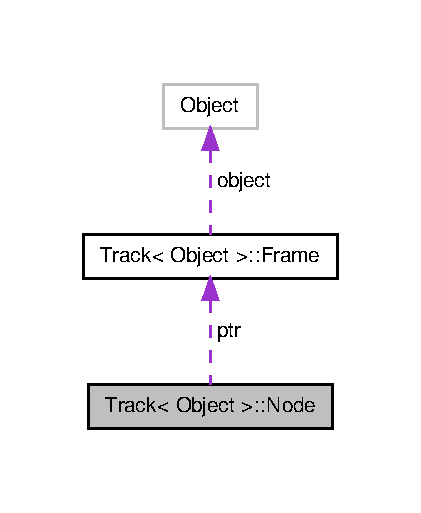
\includegraphics[width=202pt]{struct_track_1_1_node__coll__graph}
\end{center}
\end{figure}
\subsection*{\-Public \-Attributes}
\begin{DoxyCompactItemize}
\item 
\hyperlink{struct_track_1_1_frame}{\-Frame} \hyperlink{struct_track_1_1_node_ab2ede054f99dfa482e000894cdc35740}{ptr}
\item 
int \hyperlink{struct_track_1_1_node_ac7729bceaed8d441bfcf81162936e5be}{frame}
\item 
int \hyperlink{struct_track_1_1_node_aa86e28e758e2a6833d09d8653488a553}{node\-Id}
\end{DoxyCompactItemize}
\subsubsection*{template$<$class Object$>$ struct Track$<$ Object $>$\-::\-Node}



\subsection{\-Member \-Data \-Documentation}
\hypertarget{struct_track_1_1_node_ac7729bceaed8d441bfcf81162936e5be}{\index{\-Track\-::\-Node@{\-Track\-::\-Node}!frame@{frame}}
\index{frame@{frame}!Track::Node@{\-Track\-::\-Node}}
\subsubsection[{frame}]{\setlength{\rightskip}{0pt plus 5cm}template$<$class Object $>$ int {\bf \-Track}$<$ \-Object $>$\-::{\bf \-Node\-::frame}}}\label{struct_track_1_1_node_ac7729bceaed8d441bfcf81162936e5be}
\hypertarget{struct_track_1_1_node_aa86e28e758e2a6833d09d8653488a553}{\index{\-Track\-::\-Node@{\-Track\-::\-Node}!node\-Id@{node\-Id}}
\index{node\-Id@{node\-Id}!Track::Node@{\-Track\-::\-Node}}
\subsubsection[{node\-Id}]{\setlength{\rightskip}{0pt plus 5cm}template$<$class Object $>$ int {\bf \-Track}$<$ \-Object $>$\-::{\bf \-Node\-::node\-Id}}}\label{struct_track_1_1_node_aa86e28e758e2a6833d09d8653488a553}
\hypertarget{struct_track_1_1_node_ab2ede054f99dfa482e000894cdc35740}{\index{\-Track\-::\-Node@{\-Track\-::\-Node}!ptr@{ptr}}
\index{ptr@{ptr}!Track::Node@{\-Track\-::\-Node}}
\subsubsection[{ptr}]{\setlength{\rightskip}{0pt plus 5cm}template$<$class Object $>$ {\bf \-Frame} {\bf \-Track}$<$ \-Object $>$\-::{\bf \-Node\-::ptr}}}\label{struct_track_1_1_node_ab2ede054f99dfa482e000894cdc35740}


\-The documentation for this struct was generated from the following file\-:\begin{DoxyCompactItemize}
\item 
/home/koosy/koosywork/pmot\-\_\-realtime/pmot\-\_\-realtime/src/\hyperlink{track_8h}{track.\-h}\end{DoxyCompactItemize}

\hypertarget{struct_object_node}{\section{\-Object\-Node \-Struct \-Reference}
\label{struct_object_node}\index{\-Object\-Node@{\-Object\-Node}}
}


{\ttfamily \#include $<$pctracking.\-h$>$}



\-Collaboration diagram for \-Object\-Node\-:
\nopagebreak
\begin{figure}[H]
\begin{center}
\leavevmode
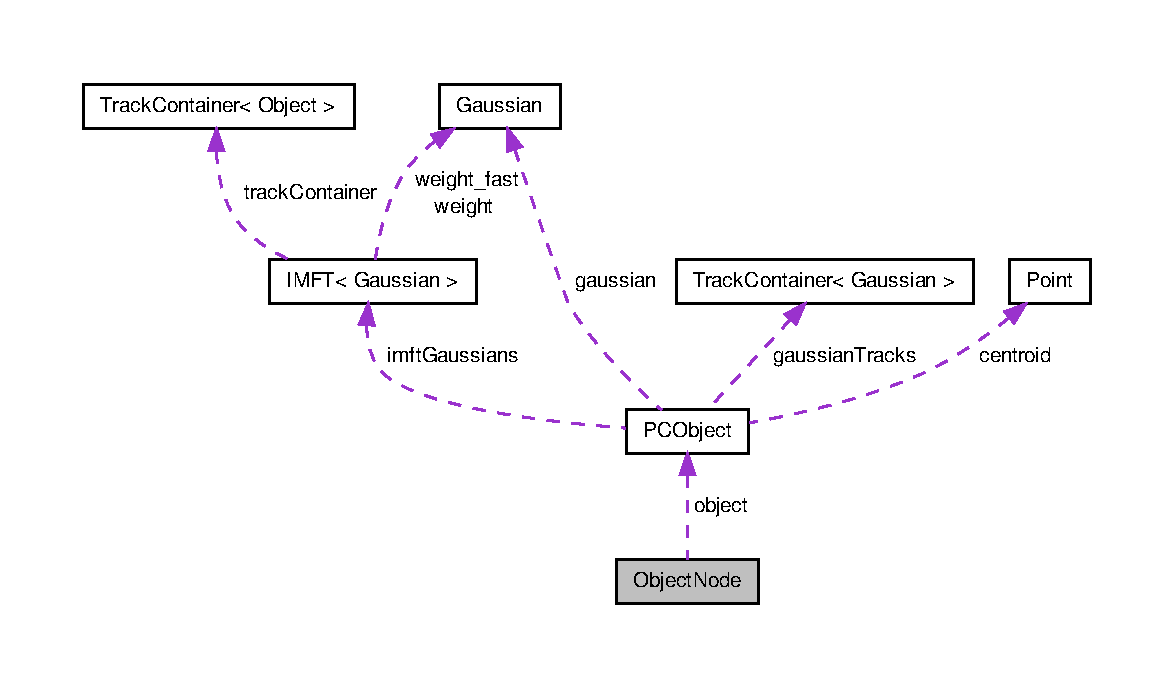
\includegraphics[width=350pt]{struct_object_node__coll__graph}
\end{center}
\end{figure}
\subsection*{\-Public \-Attributes}
\begin{DoxyCompactItemize}
\item 
\hyperlink{pctracking_8h_a1d1cfd8ffb84e947f82999c682b666a7}{\-Type} \hyperlink{struct_object_node_a5afed3ebe97aa3a945f29934532b5154}{type}
\item 
\hyperlink{pctracking_8h_a80b0d67eccd8a722b335bc1c9679a2f7}{\-Time} \hyperlink{struct_object_node_a436ab00d9951d27c758081bad6c9d690}{time}
\item 
\hyperlink{class_p_c_object}{\-P\-C\-Object} \hyperlink{struct_object_node_a9e1e36a7fe384526cb99ceddfd86e598}{object}
\item 
int \hyperlink{struct_object_node_a07820c0eda571bedfac7a04171c4786e}{n\-Out}
\item 
int \hyperlink{struct_object_node_a10f5902c1668612e39b46150894bd0f9}{n\-In}
\end{DoxyCompactItemize}


\subsection{\-Member \-Data \-Documentation}
\hypertarget{struct_object_node_a10f5902c1668612e39b46150894bd0f9}{\index{\-Object\-Node@{\-Object\-Node}!n\-In@{n\-In}}
\index{n\-In@{n\-In}!ObjectNode@{\-Object\-Node}}
\subsubsection[{n\-In}]{\setlength{\rightskip}{0pt plus 5cm}int {\bf \-Object\-Node\-::n\-In}}}\label{struct_object_node_a10f5902c1668612e39b46150894bd0f9}
\hypertarget{struct_object_node_a07820c0eda571bedfac7a04171c4786e}{\index{\-Object\-Node@{\-Object\-Node}!n\-Out@{n\-Out}}
\index{n\-Out@{n\-Out}!ObjectNode@{\-Object\-Node}}
\subsubsection[{n\-Out}]{\setlength{\rightskip}{0pt plus 5cm}int {\bf \-Object\-Node\-::n\-Out}}}\label{struct_object_node_a07820c0eda571bedfac7a04171c4786e}
\hypertarget{struct_object_node_a9e1e36a7fe384526cb99ceddfd86e598}{\index{\-Object\-Node@{\-Object\-Node}!object@{object}}
\index{object@{object}!ObjectNode@{\-Object\-Node}}
\subsubsection[{object}]{\setlength{\rightskip}{0pt plus 5cm}{\bf \-P\-C\-Object} {\bf \-Object\-Node\-::object}}}\label{struct_object_node_a9e1e36a7fe384526cb99ceddfd86e598}
\hypertarget{struct_object_node_a436ab00d9951d27c758081bad6c9d690}{\index{\-Object\-Node@{\-Object\-Node}!time@{time}}
\index{time@{time}!ObjectNode@{\-Object\-Node}}
\subsubsection[{time}]{\setlength{\rightskip}{0pt plus 5cm}{\bf \-Time} {\bf \-Object\-Node\-::time}}}\label{struct_object_node_a436ab00d9951d27c758081bad6c9d690}
\hypertarget{struct_object_node_a5afed3ebe97aa3a945f29934532b5154}{\index{\-Object\-Node@{\-Object\-Node}!type@{type}}
\index{type@{type}!ObjectNode@{\-Object\-Node}}
\subsubsection[{type}]{\setlength{\rightskip}{0pt plus 5cm}{\bf \-Type} {\bf \-Object\-Node\-::type}}}\label{struct_object_node_a5afed3ebe97aa3a945f29934532b5154}


\-The documentation for this struct was generated from the following file\-:\begin{DoxyCompactItemize}
\item 
/home/koosy/koosywork/pmot\-\_\-realtime/pmot\-\_\-realtime/src/\hyperlink{pctracking_8h}{pctracking.\-h}\end{DoxyCompactItemize}

\hypertarget{class_particlepose}{\section{\-Particlepose \-Class \-Reference}
\label{class_particlepose}\index{\-Particlepose@{\-Particlepose}}
}


{\ttfamily \#include $<$particlepose.\-h$>$}



\-Collaboration diagram for \-Particlepose\-:
\nopagebreak
\begin{figure}[H]
\begin{center}
\leavevmode
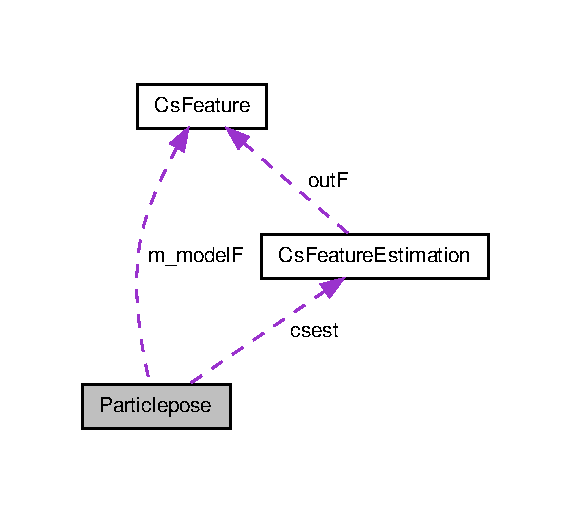
\includegraphics[width=274pt]{class_particlepose__coll__graph}
\end{center}
\end{figure}
\subsection*{\-Public \-Member \-Functions}
\begin{DoxyCompactItemize}
\item 
\hyperlink{class_particlepose_ad0812c3c3ae574cd927f25980d63262c}{\-Particlepose} ()
\item 
\hyperlink{class_particlepose_a3a6c9be74fe45665ba536de53a91d268}{$\sim$\-Particlepose} ()
\item 
void \hyperlink{class_particlepose_ad32cef58fb6f06fc41332170241ad132}{setdata} (\hyperlink{common_8h_a36884aa4a3c181fa4c284d79329ad166}{\-Cloud\-Ptr} scene, \hyperlink{common_8h_a36884aa4a3c181fa4c284d79329ad166}{\-Cloud\-Ptr} model, int cnt)
\item 
\hyperlink{common_8h_a36884aa4a3c181fa4c284d79329ad166}{\-Cloud\-Ptr} \hyperlink{class_particlepose_ad3ff7daa451218d902b0bffcf5c4e5bc}{get\-Result} ()
\item 
void \hyperlink{class_particlepose_ab579314deee0989210524ac33a0507e5}{init\-Sample} ()
\item 
void \hyperlink{class_particlepose_af5322a5db6b412a5a057c687511424ef}{resample} (float var\-Dist, float var\-Ang)
\item 
void \hyperlink{class_particlepose_a5969de8804b86d863d03eaf2b2f24480}{weight} ()
\item 
\hyperlink{common_8h_a36884aa4a3c181fa4c284d79329ad166}{\-Cloud\-Ptr} \hyperlink{class_particlepose_a719e82e44ddb312a54f6728afa6300ec}{to\-Cloud} ()
\item 
void \hyperlink{class_particlepose_a58a07a0b87e10acbf73de973e8dd9618}{update\-Model} (\hyperlink{common_8h_a36884aa4a3c181fa4c284d79329ad166}{\-Cloud\-Ptr} cloud)
\item 
std\-::vector$<$ float $>$ \hyperlink{class_particlepose_a2dfff2c77bd7367a0413cbb463c2986a}{weight\-G\-P\-U} (float gridsize, int xnr, int ynr, int znr, \-Vector4f min, \-Vector4f max, std\-::vector$<$ float $>$ refhist)
\item 
float \hyperlink{class_particlepose_a37277d19b404d2dc338f56ff98049868}{distfeature} (\-V\-F\-H\-Signature308 f1, \-V\-F\-H\-Signature308 f2)
\item 
void \hyperlink{class_particlepose_af53e0c58df04f1cc6edaea13f6530d05}{weight\-By\-Dist} ()
\item 
std\-::vector$<$ float $>$ \hyperlink{class_particlepose_ad42796cd810c3d078604c8a286fe90bd}{get\-Patch\-Score} (\hyperlink{common_8h_a36884aa4a3c181fa4c284d79329ad166}{\-Cloud\-Ptr} cloud)
\end{DoxyCompactItemize}
\subsection*{\-Public \-Attributes}
\begin{DoxyCompactItemize}
\item 
\hyperlink{class_cs_feature}{\-Cs\-Feature} \hyperlink{class_particlepose_a4d0304244af04da649472549e3a57f05}{m\-\_\-model\-F}
\item 
\hyperlink{class_cs_feature_estimation}{\-Cs\-Feature\-Estimation} \hyperlink{class_particlepose_af41bfccd67a035c391b1e4655d66f631}{csest}
\end{DoxyCompactItemize}
\subsection*{\-Private \-Member \-Functions}
\begin{DoxyCompactItemize}
\item 
tracking\-::\-Particle\-X\-Y\-Z\-R\-P\-Y \hyperlink{class_particlepose_a248a7f70bff04020c78dca31c3d35053}{sample\-With\-Var} (tracking\-::\-Particle\-X\-Y\-Z\-R\-P\-Y part, float var\-Dist, float var\-Ang)
\end{DoxyCompactItemize}
\subsection*{\-Private \-Attributes}
\begin{DoxyCompactItemize}
\item 
boost\-::mt19937 \hyperlink{class_particlepose_a0449123f3b8952410023d15b202be7a5}{m\-\_\-gen}
\item 
tracking\-::\-Particle\-X\-Y\-Z\-R\-P\-Y \hyperlink{class_particlepose_ac013ac13e2a6c5a676714a4a9bccd8c1}{m\-\_\-final\-Particle}
\item 
tracking\-::\-Particle\-X\-Y\-Z\-R\-P\-Y \hyperlink{class_particlepose_a1b1424c075e6c1010d02cb558b26a1e3}{m\-\_\-last\-Final\-Particle}
\item 
tracking\-::\-Particle\-X\-Y\-Z\-R\-P\-Y \hyperlink{class_particlepose_acbd0492a1807c3e7c8be11b89549084d}{m\-\_\-lastlast\-Final\-Particle}
\item 
tracking\-::\-Particle\-X\-Y\-Z\-R\-P\-Y \hyperlink{class_particlepose_a6397839aacb6f69e3230596cfa6f79c7}{m\-\_\-lastlastlast\-Final\-Particle}
\item 
tracking\-::\-Particle\-X\-Y\-Z\-R\-P\-Y \hyperlink{class_particlepose_a524fa648db6f575f6c8891d11863d3f0}{m\-\_\-vel}
\item 
tracking\-::\-Particle\-X\-Y\-Z\-R\-P\-Y \hyperlink{class_particlepose_af03fc2a655e8d55116285f7c6b84b008}{m\-\_\-acc}
\item 
\-Eigen\-::\-Vector4f \hyperlink{class_particlepose_a15f08163cf8864a6536cb3eee81aaacd}{m\-\_\-scene\-Centroid}
\item 
\-Eigen\-::\-Vector4f \hyperlink{class_particlepose_aa5617380ebdece16240b76b515fb4fee}{m\-\_\-model\-Centroid}
\item 
pcl\-::gpu\-::\-Octree \hyperlink{class_particlepose_ab0559e3d6171dd3cec9eddb9b5992c62}{m\-\_\-octreegpu}
\item 
\hyperlink{common_8h_a36884aa4a3c181fa4c284d79329ad166}{\-Cloud\-Ptr} \hyperlink{class_particlepose_a8b8ba753e0f7624ad67097faf454d9ba}{m\-\_\-scene}
\item 
\hyperlink{common_8h_a36884aa4a3c181fa4c284d79329ad166}{\-Cloud\-Ptr} \hyperlink{class_particlepose_a392f6b998bbda4e33561669cb9a8bac0}{m\-\_\-model}
\item 
\hyperlink{common_8h_a36884aa4a3c181fa4c284d79329ad166}{\-Cloud\-Ptr} \hyperlink{class_particlepose_a2911816a0cc8e02c4190d028f32a0b9d}{m\-\_\-model\-Orig}
\item 
\hyperlink{common_8h_ac29cd61ffd2436715a9b935fe2122703}{\-Cloud\-N\-Ptr} \hyperlink{class_particlepose_a29c9f00444dd5ed1e42cdd8536873e90}{m\-\_\-scene\-N}
\item 
\hyperlink{common_8h_ac29cd61ffd2436715a9b935fe2122703}{\-Cloud\-N\-Ptr} \hyperlink{class_particlepose_a6fcd5ba77748ec02218592201874bb75}{m\-\_\-model\-N}
\item 
int \hyperlink{class_particlepose_afbda237928cf27273f3c8e0ac8cb0d2f}{m\-\_\-particlenum}
\item 
std\-::vector\*
$<$ tracking\-::\-Particle\-X\-Y\-Z\-R\-P\-Y $>$ \hyperlink{class_particlepose_a6e0d2bdcd0131039227ccf35ef42d65e}{m\-\_\-particles}
\item 
std\-::vector\*
$<$ tracking\-::\-Particle\-X\-Y\-Z\-R\-P\-Y $>$ \hyperlink{class_particlepose_a0c1673111cdab70b548a9ce5a5cbf8bf}{m\-\_\-lastspeed}
\item 
std\-::vector\*
$<$ tracking\-::\-Particle\-X\-Y\-Z\-R\-P\-Y $>$ \hyperlink{class_particlepose_a555761b64f69c60d7633a30013e0e422}{m\-\_\-bestspeed}
\item 
pcl\-::\-Kd\-Tree\-F\-L\-A\-N\-N$<$ \hyperlink{common_8h_a4201c2c72d96e356cbee6fefdaf8da6a}{\-Point\-N\-T} $>$\-::\-Ptr \hyperlink{class_particlepose_ad68d6c6cb6c98cd908a3e9e903fdbac5}{m\-\_\-kdtree\-Scene\-N}
\item 
int \hyperlink{class_particlepose_aab1bfddc21050cc4e1ffedd146b4bbaa}{m\-\_\-cnt}
\item 
int \hyperlink{class_particlepose_aa4b1d0fe4fc48e68039ee1e9b2cb93dd}{m\-\_\-internal\-Counter}
\item 
float \hyperlink{class_particlepose_a827812bbc2da3926fd03c1a7e8e4e287}{min\-Dist}
\item 
float \hyperlink{class_particlepose_a5cbcf40f5baa980ff3d948e8f644fda1}{max\-Dist}
\item 
bool \hyperlink{class_particlepose_ac70adde4c1af0773ec887721283b98db}{usegpu}
\end{DoxyCompactItemize}


\subsection{\-Constructor \& \-Destructor \-Documentation}
\hypertarget{class_particlepose_ad0812c3c3ae574cd927f25980d63262c}{\index{\-Particlepose@{\-Particlepose}!\-Particlepose@{\-Particlepose}}
\index{\-Particlepose@{\-Particlepose}!Particlepose@{\-Particlepose}}
\subsubsection[{\-Particlepose}]{\setlength{\rightskip}{0pt plus 5cm}{\bf \-Particlepose\-::\-Particlepose} (
\begin{DoxyParamCaption}
{}
\end{DoxyParamCaption}
)}}\label{class_particlepose_ad0812c3c3ae574cd927f25980d63262c}
\hypertarget{class_particlepose_a3a6c9be74fe45665ba536de53a91d268}{\index{\-Particlepose@{\-Particlepose}!$\sim$\-Particlepose@{$\sim$\-Particlepose}}
\index{$\sim$\-Particlepose@{$\sim$\-Particlepose}!Particlepose@{\-Particlepose}}
\subsubsection[{$\sim$\-Particlepose}]{\setlength{\rightskip}{0pt plus 5cm}{\bf \-Particlepose\-::$\sim$\-Particlepose} (
\begin{DoxyParamCaption}
{}
\end{DoxyParamCaption}
)}}\label{class_particlepose_a3a6c9be74fe45665ba536de53a91d268}


\subsection{\-Member \-Function \-Documentation}
\hypertarget{class_particlepose_a37277d19b404d2dc338f56ff98049868}{\index{\-Particlepose@{\-Particlepose}!distfeature@{distfeature}}
\index{distfeature@{distfeature}!Particlepose@{\-Particlepose}}
\subsubsection[{distfeature}]{\setlength{\rightskip}{0pt plus 5cm}float {\bf \-Particlepose\-::distfeature} (
\begin{DoxyParamCaption}
\item[{\-V\-F\-H\-Signature308}]{f1, }
\item[{\-V\-F\-H\-Signature308}]{f2}
\end{DoxyParamCaption}
)}}\label{class_particlepose_a37277d19b404d2dc338f56ff98049868}
\hypertarget{class_particlepose_ad42796cd810c3d078604c8a286fe90bd}{\index{\-Particlepose@{\-Particlepose}!get\-Patch\-Score@{get\-Patch\-Score}}
\index{get\-Patch\-Score@{get\-Patch\-Score}!Particlepose@{\-Particlepose}}
\subsubsection[{get\-Patch\-Score}]{\setlength{\rightskip}{0pt plus 5cm}std\-::vector$<$ float $>$ {\bf \-Particlepose\-::get\-Patch\-Score} (
\begin{DoxyParamCaption}
\item[{{\bf \-Cloud\-Ptr}}]{cloud}
\end{DoxyParamCaption}
)}}\label{class_particlepose_ad42796cd810c3d078604c8a286fe90bd}
\hypertarget{class_particlepose_ad3ff7daa451218d902b0bffcf5c4e5bc}{\index{\-Particlepose@{\-Particlepose}!get\-Result@{get\-Result}}
\index{get\-Result@{get\-Result}!Particlepose@{\-Particlepose}}
\subsubsection[{get\-Result}]{\setlength{\rightskip}{0pt plus 5cm}{\bf \-Cloud\-Ptr} {\bf \-Particlepose\-::get\-Result} (
\begin{DoxyParamCaption}
{}
\end{DoxyParamCaption}
)}}\label{class_particlepose_ad3ff7daa451218d902b0bffcf5c4e5bc}
\hypertarget{class_particlepose_ab579314deee0989210524ac33a0507e5}{\index{\-Particlepose@{\-Particlepose}!init\-Sample@{init\-Sample}}
\index{init\-Sample@{init\-Sample}!Particlepose@{\-Particlepose}}
\subsubsection[{init\-Sample}]{\setlength{\rightskip}{0pt plus 5cm}void {\bf \-Particlepose\-::init\-Sample} (
\begin{DoxyParamCaption}
{}
\end{DoxyParamCaption}
)}}\label{class_particlepose_ab579314deee0989210524ac33a0507e5}
\hypertarget{class_particlepose_af5322a5db6b412a5a057c687511424ef}{\index{\-Particlepose@{\-Particlepose}!resample@{resample}}
\index{resample@{resample}!Particlepose@{\-Particlepose}}
\subsubsection[{resample}]{\setlength{\rightskip}{0pt plus 5cm}void {\bf \-Particlepose\-::resample} (
\begin{DoxyParamCaption}
\item[{float}]{var\-Dist, }
\item[{float}]{var\-Ang}
\end{DoxyParamCaption}
)}}\label{class_particlepose_af5322a5db6b412a5a057c687511424ef}
\hypertarget{class_particlepose_a248a7f70bff04020c78dca31c3d35053}{\index{\-Particlepose@{\-Particlepose}!sample\-With\-Var@{sample\-With\-Var}}
\index{sample\-With\-Var@{sample\-With\-Var}!Particlepose@{\-Particlepose}}
\subsubsection[{sample\-With\-Var}]{\setlength{\rightskip}{0pt plus 5cm}tracking\-::\-Particle\-X\-Y\-Z\-R\-P\-Y {\bf \-Particlepose\-::sample\-With\-Var} (
\begin{DoxyParamCaption}
\item[{tracking\-::\-Particle\-X\-Y\-Z\-R\-P\-Y}]{part, }
\item[{float}]{var\-Dist, }
\item[{float}]{var\-Ang}
\end{DoxyParamCaption}
)\hspace{0.3cm}{\ttfamily  \mbox{[}private\mbox{]}}}}\label{class_particlepose_a248a7f70bff04020c78dca31c3d35053}
\hypertarget{class_particlepose_ad32cef58fb6f06fc41332170241ad132}{\index{\-Particlepose@{\-Particlepose}!setdata@{setdata}}
\index{setdata@{setdata}!Particlepose@{\-Particlepose}}
\subsubsection[{setdata}]{\setlength{\rightskip}{0pt plus 5cm}void {\bf \-Particlepose\-::setdata} (
\begin{DoxyParamCaption}
\item[{{\bf \-Cloud\-Ptr}}]{scene, }
\item[{{\bf \-Cloud\-Ptr}}]{model, }
\item[{int}]{cnt}
\end{DoxyParamCaption}
)}}\label{class_particlepose_ad32cef58fb6f06fc41332170241ad132}
\hypertarget{class_particlepose_a719e82e44ddb312a54f6728afa6300ec}{\index{\-Particlepose@{\-Particlepose}!to\-Cloud@{to\-Cloud}}
\index{to\-Cloud@{to\-Cloud}!Particlepose@{\-Particlepose}}
\subsubsection[{to\-Cloud}]{\setlength{\rightskip}{0pt plus 5cm}{\bf \-Cloud\-Ptr} {\bf \-Particlepose\-::to\-Cloud} (
\begin{DoxyParamCaption}
{}
\end{DoxyParamCaption}
)}}\label{class_particlepose_a719e82e44ddb312a54f6728afa6300ec}
\hypertarget{class_particlepose_a58a07a0b87e10acbf73de973e8dd9618}{\index{\-Particlepose@{\-Particlepose}!update\-Model@{update\-Model}}
\index{update\-Model@{update\-Model}!Particlepose@{\-Particlepose}}
\subsubsection[{update\-Model}]{\setlength{\rightskip}{0pt plus 5cm}void {\bf \-Particlepose\-::update\-Model} (
\begin{DoxyParamCaption}
\item[{{\bf \-Cloud\-Ptr}}]{cloud}
\end{DoxyParamCaption}
)}}\label{class_particlepose_a58a07a0b87e10acbf73de973e8dd9618}
\hypertarget{class_particlepose_a5969de8804b86d863d03eaf2b2f24480}{\index{\-Particlepose@{\-Particlepose}!weight@{weight}}
\index{weight@{weight}!Particlepose@{\-Particlepose}}
\subsubsection[{weight}]{\setlength{\rightskip}{0pt plus 5cm}void {\bf \-Particlepose\-::weight} (
\begin{DoxyParamCaption}
{}
\end{DoxyParamCaption}
)}}\label{class_particlepose_a5969de8804b86d863d03eaf2b2f24480}


\-Here is the call graph for this function\-:
\nopagebreak
\begin{figure}[H]
\begin{center}
\leavevmode
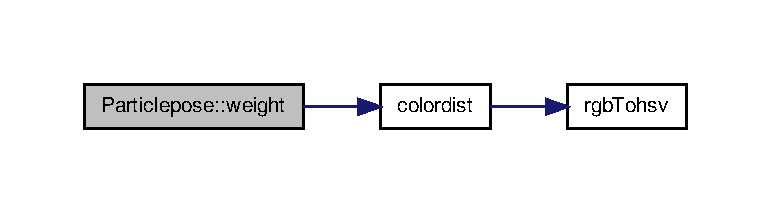
\includegraphics[width=350pt]{class_particlepose_a5969de8804b86d863d03eaf2b2f24480_cgraph}
\end{center}
\end{figure}


\hypertarget{class_particlepose_af53e0c58df04f1cc6edaea13f6530d05}{\index{\-Particlepose@{\-Particlepose}!weight\-By\-Dist@{weight\-By\-Dist}}
\index{weight\-By\-Dist@{weight\-By\-Dist}!Particlepose@{\-Particlepose}}
\subsubsection[{weight\-By\-Dist}]{\setlength{\rightskip}{0pt plus 5cm}void {\bf \-Particlepose\-::weight\-By\-Dist} (
\begin{DoxyParamCaption}
{}
\end{DoxyParamCaption}
)\hspace{0.3cm}{\ttfamily  \mbox{[}inline\mbox{]}}}}\label{class_particlepose_af53e0c58df04f1cc6edaea13f6530d05}
\hypertarget{class_particlepose_a2dfff2c77bd7367a0413cbb463c2986a}{\index{\-Particlepose@{\-Particlepose}!weight\-G\-P\-U@{weight\-G\-P\-U}}
\index{weight\-G\-P\-U@{weight\-G\-P\-U}!Particlepose@{\-Particlepose}}
\subsubsection[{weight\-G\-P\-U}]{\setlength{\rightskip}{0pt plus 5cm}std\-::vector$<$ float $>$ {\bf \-Particlepose\-::weight\-G\-P\-U} (
\begin{DoxyParamCaption}
\item[{float}]{gridsize, }
\item[{int}]{xnr, }
\item[{int}]{ynr, }
\item[{int}]{znr, }
\item[{\-Vector4f}]{min, }
\item[{\-Vector4f}]{max, }
\item[{std\-::vector$<$ float $>$}]{refhist}
\end{DoxyParamCaption}
)}}\label{class_particlepose_a2dfff2c77bd7367a0413cbb463c2986a}


\-Here is the call graph for this function\-:
\nopagebreak
\begin{figure}[H]
\begin{center}
\leavevmode
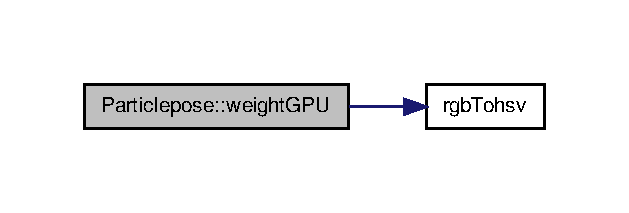
\includegraphics[width=302pt]{class_particlepose_a2dfff2c77bd7367a0413cbb463c2986a_cgraph}
\end{center}
\end{figure}




\subsection{\-Member \-Data \-Documentation}
\hypertarget{class_particlepose_af41bfccd67a035c391b1e4655d66f631}{\index{\-Particlepose@{\-Particlepose}!csest@{csest}}
\index{csest@{csest}!Particlepose@{\-Particlepose}}
\subsubsection[{csest}]{\setlength{\rightskip}{0pt plus 5cm}{\bf \-Cs\-Feature\-Estimation} {\bf \-Particlepose\-::csest}}}\label{class_particlepose_af41bfccd67a035c391b1e4655d66f631}
\hypertarget{class_particlepose_af03fc2a655e8d55116285f7c6b84b008}{\index{\-Particlepose@{\-Particlepose}!m\-\_\-acc@{m\-\_\-acc}}
\index{m\-\_\-acc@{m\-\_\-acc}!Particlepose@{\-Particlepose}}
\subsubsection[{m\-\_\-acc}]{\setlength{\rightskip}{0pt plus 5cm}tracking\-::\-Particle\-X\-Y\-Z\-R\-P\-Y {\bf \-Particlepose\-::m\-\_\-acc}\hspace{0.3cm}{\ttfamily  \mbox{[}private\mbox{]}}}}\label{class_particlepose_af03fc2a655e8d55116285f7c6b84b008}
\hypertarget{class_particlepose_a555761b64f69c60d7633a30013e0e422}{\index{\-Particlepose@{\-Particlepose}!m\-\_\-bestspeed@{m\-\_\-bestspeed}}
\index{m\-\_\-bestspeed@{m\-\_\-bestspeed}!Particlepose@{\-Particlepose}}
\subsubsection[{m\-\_\-bestspeed}]{\setlength{\rightskip}{0pt plus 5cm}std\-::vector$<$tracking\-::\-Particle\-X\-Y\-Z\-R\-P\-Y$>$ {\bf \-Particlepose\-::m\-\_\-bestspeed}\hspace{0.3cm}{\ttfamily  \mbox{[}private\mbox{]}}}}\label{class_particlepose_a555761b64f69c60d7633a30013e0e422}
\hypertarget{class_particlepose_aab1bfddc21050cc4e1ffedd146b4bbaa}{\index{\-Particlepose@{\-Particlepose}!m\-\_\-cnt@{m\-\_\-cnt}}
\index{m\-\_\-cnt@{m\-\_\-cnt}!Particlepose@{\-Particlepose}}
\subsubsection[{m\-\_\-cnt}]{\setlength{\rightskip}{0pt plus 5cm}int {\bf \-Particlepose\-::m\-\_\-cnt}\hspace{0.3cm}{\ttfamily  \mbox{[}private\mbox{]}}}}\label{class_particlepose_aab1bfddc21050cc4e1ffedd146b4bbaa}
\hypertarget{class_particlepose_ac013ac13e2a6c5a676714a4a9bccd8c1}{\index{\-Particlepose@{\-Particlepose}!m\-\_\-final\-Particle@{m\-\_\-final\-Particle}}
\index{m\-\_\-final\-Particle@{m\-\_\-final\-Particle}!Particlepose@{\-Particlepose}}
\subsubsection[{m\-\_\-final\-Particle}]{\setlength{\rightskip}{0pt plus 5cm}tracking\-::\-Particle\-X\-Y\-Z\-R\-P\-Y {\bf \-Particlepose\-::m\-\_\-final\-Particle}\hspace{0.3cm}{\ttfamily  \mbox{[}private\mbox{]}}}}\label{class_particlepose_ac013ac13e2a6c5a676714a4a9bccd8c1}
\hypertarget{class_particlepose_a0449123f3b8952410023d15b202be7a5}{\index{\-Particlepose@{\-Particlepose}!m\-\_\-gen@{m\-\_\-gen}}
\index{m\-\_\-gen@{m\-\_\-gen}!Particlepose@{\-Particlepose}}
\subsubsection[{m\-\_\-gen}]{\setlength{\rightskip}{0pt plus 5cm}boost\-::mt19937 {\bf \-Particlepose\-::m\-\_\-gen}\hspace{0.3cm}{\ttfamily  \mbox{[}private\mbox{]}}}}\label{class_particlepose_a0449123f3b8952410023d15b202be7a5}
\hypertarget{class_particlepose_aa4b1d0fe4fc48e68039ee1e9b2cb93dd}{\index{\-Particlepose@{\-Particlepose}!m\-\_\-internal\-Counter@{m\-\_\-internal\-Counter}}
\index{m\-\_\-internal\-Counter@{m\-\_\-internal\-Counter}!Particlepose@{\-Particlepose}}
\subsubsection[{m\-\_\-internal\-Counter}]{\setlength{\rightskip}{0pt plus 5cm}int {\bf \-Particlepose\-::m\-\_\-internal\-Counter}\hspace{0.3cm}{\ttfamily  \mbox{[}private\mbox{]}}}}\label{class_particlepose_aa4b1d0fe4fc48e68039ee1e9b2cb93dd}
\hypertarget{class_particlepose_ad68d6c6cb6c98cd908a3e9e903fdbac5}{\index{\-Particlepose@{\-Particlepose}!m\-\_\-kdtree\-Scene\-N@{m\-\_\-kdtree\-Scene\-N}}
\index{m\-\_\-kdtree\-Scene\-N@{m\-\_\-kdtree\-Scene\-N}!Particlepose@{\-Particlepose}}
\subsubsection[{m\-\_\-kdtree\-Scene\-N}]{\setlength{\rightskip}{0pt plus 5cm}pcl\-::\-Kd\-Tree\-F\-L\-A\-N\-N$<${\bf \-Point\-N\-T}$>$\-::\-Ptr {\bf \-Particlepose\-::m\-\_\-kdtree\-Scene\-N}\hspace{0.3cm}{\ttfamily  \mbox{[}private\mbox{]}}}}\label{class_particlepose_ad68d6c6cb6c98cd908a3e9e903fdbac5}
\hypertarget{class_particlepose_a1b1424c075e6c1010d02cb558b26a1e3}{\index{\-Particlepose@{\-Particlepose}!m\-\_\-last\-Final\-Particle@{m\-\_\-last\-Final\-Particle}}
\index{m\-\_\-last\-Final\-Particle@{m\-\_\-last\-Final\-Particle}!Particlepose@{\-Particlepose}}
\subsubsection[{m\-\_\-last\-Final\-Particle}]{\setlength{\rightskip}{0pt plus 5cm}tracking\-::\-Particle\-X\-Y\-Z\-R\-P\-Y {\bf \-Particlepose\-::m\-\_\-last\-Final\-Particle}\hspace{0.3cm}{\ttfamily  \mbox{[}private\mbox{]}}}}\label{class_particlepose_a1b1424c075e6c1010d02cb558b26a1e3}
\hypertarget{class_particlepose_acbd0492a1807c3e7c8be11b89549084d}{\index{\-Particlepose@{\-Particlepose}!m\-\_\-lastlast\-Final\-Particle@{m\-\_\-lastlast\-Final\-Particle}}
\index{m\-\_\-lastlast\-Final\-Particle@{m\-\_\-lastlast\-Final\-Particle}!Particlepose@{\-Particlepose}}
\subsubsection[{m\-\_\-lastlast\-Final\-Particle}]{\setlength{\rightskip}{0pt plus 5cm}tracking\-::\-Particle\-X\-Y\-Z\-R\-P\-Y {\bf \-Particlepose\-::m\-\_\-lastlast\-Final\-Particle}\hspace{0.3cm}{\ttfamily  \mbox{[}private\mbox{]}}}}\label{class_particlepose_acbd0492a1807c3e7c8be11b89549084d}
\hypertarget{class_particlepose_a6397839aacb6f69e3230596cfa6f79c7}{\index{\-Particlepose@{\-Particlepose}!m\-\_\-lastlastlast\-Final\-Particle@{m\-\_\-lastlastlast\-Final\-Particle}}
\index{m\-\_\-lastlastlast\-Final\-Particle@{m\-\_\-lastlastlast\-Final\-Particle}!Particlepose@{\-Particlepose}}
\subsubsection[{m\-\_\-lastlastlast\-Final\-Particle}]{\setlength{\rightskip}{0pt plus 5cm}tracking\-::\-Particle\-X\-Y\-Z\-R\-P\-Y {\bf \-Particlepose\-::m\-\_\-lastlastlast\-Final\-Particle}\hspace{0.3cm}{\ttfamily  \mbox{[}private\mbox{]}}}}\label{class_particlepose_a6397839aacb6f69e3230596cfa6f79c7}
\hypertarget{class_particlepose_a0c1673111cdab70b548a9ce5a5cbf8bf}{\index{\-Particlepose@{\-Particlepose}!m\-\_\-lastspeed@{m\-\_\-lastspeed}}
\index{m\-\_\-lastspeed@{m\-\_\-lastspeed}!Particlepose@{\-Particlepose}}
\subsubsection[{m\-\_\-lastspeed}]{\setlength{\rightskip}{0pt plus 5cm}std\-::vector$<$tracking\-::\-Particle\-X\-Y\-Z\-R\-P\-Y$>$ {\bf \-Particlepose\-::m\-\_\-lastspeed}\hspace{0.3cm}{\ttfamily  \mbox{[}private\mbox{]}}}}\label{class_particlepose_a0c1673111cdab70b548a9ce5a5cbf8bf}
\hypertarget{class_particlepose_a392f6b998bbda4e33561669cb9a8bac0}{\index{\-Particlepose@{\-Particlepose}!m\-\_\-model@{m\-\_\-model}}
\index{m\-\_\-model@{m\-\_\-model}!Particlepose@{\-Particlepose}}
\subsubsection[{m\-\_\-model}]{\setlength{\rightskip}{0pt plus 5cm}{\bf \-Cloud\-Ptr} {\bf \-Particlepose\-::m\-\_\-model}\hspace{0.3cm}{\ttfamily  \mbox{[}private\mbox{]}}}}\label{class_particlepose_a392f6b998bbda4e33561669cb9a8bac0}
\hypertarget{class_particlepose_aa5617380ebdece16240b76b515fb4fee}{\index{\-Particlepose@{\-Particlepose}!m\-\_\-model\-Centroid@{m\-\_\-model\-Centroid}}
\index{m\-\_\-model\-Centroid@{m\-\_\-model\-Centroid}!Particlepose@{\-Particlepose}}
\subsubsection[{m\-\_\-model\-Centroid}]{\setlength{\rightskip}{0pt plus 5cm}\-Eigen\-::\-Vector4f {\bf \-Particlepose\-::m\-\_\-model\-Centroid}\hspace{0.3cm}{\ttfamily  \mbox{[}private\mbox{]}}}}\label{class_particlepose_aa5617380ebdece16240b76b515fb4fee}
\hypertarget{class_particlepose_a4d0304244af04da649472549e3a57f05}{\index{\-Particlepose@{\-Particlepose}!m\-\_\-model\-F@{m\-\_\-model\-F}}
\index{m\-\_\-model\-F@{m\-\_\-model\-F}!Particlepose@{\-Particlepose}}
\subsubsection[{m\-\_\-model\-F}]{\setlength{\rightskip}{0pt plus 5cm}{\bf \-Cs\-Feature} {\bf \-Particlepose\-::m\-\_\-model\-F}}}\label{class_particlepose_a4d0304244af04da649472549e3a57f05}
\hypertarget{class_particlepose_a6fcd5ba77748ec02218592201874bb75}{\index{\-Particlepose@{\-Particlepose}!m\-\_\-model\-N@{m\-\_\-model\-N}}
\index{m\-\_\-model\-N@{m\-\_\-model\-N}!Particlepose@{\-Particlepose}}
\subsubsection[{m\-\_\-model\-N}]{\setlength{\rightskip}{0pt plus 5cm}{\bf \-Cloud\-N\-Ptr} {\bf \-Particlepose\-::m\-\_\-model\-N}\hspace{0.3cm}{\ttfamily  \mbox{[}private\mbox{]}}}}\label{class_particlepose_a6fcd5ba77748ec02218592201874bb75}
\hypertarget{class_particlepose_a2911816a0cc8e02c4190d028f32a0b9d}{\index{\-Particlepose@{\-Particlepose}!m\-\_\-model\-Orig@{m\-\_\-model\-Orig}}
\index{m\-\_\-model\-Orig@{m\-\_\-model\-Orig}!Particlepose@{\-Particlepose}}
\subsubsection[{m\-\_\-model\-Orig}]{\setlength{\rightskip}{0pt plus 5cm}{\bf \-Cloud\-Ptr} {\bf \-Particlepose\-::m\-\_\-model\-Orig}\hspace{0.3cm}{\ttfamily  \mbox{[}private\mbox{]}}}}\label{class_particlepose_a2911816a0cc8e02c4190d028f32a0b9d}
\hypertarget{class_particlepose_ab0559e3d6171dd3cec9eddb9b5992c62}{\index{\-Particlepose@{\-Particlepose}!m\-\_\-octreegpu@{m\-\_\-octreegpu}}
\index{m\-\_\-octreegpu@{m\-\_\-octreegpu}!Particlepose@{\-Particlepose}}
\subsubsection[{m\-\_\-octreegpu}]{\setlength{\rightskip}{0pt plus 5cm}pcl\-::gpu\-::\-Octree {\bf \-Particlepose\-::m\-\_\-octreegpu}\hspace{0.3cm}{\ttfamily  \mbox{[}private\mbox{]}}}}\label{class_particlepose_ab0559e3d6171dd3cec9eddb9b5992c62}
\hypertarget{class_particlepose_afbda237928cf27273f3c8e0ac8cb0d2f}{\index{\-Particlepose@{\-Particlepose}!m\-\_\-particlenum@{m\-\_\-particlenum}}
\index{m\-\_\-particlenum@{m\-\_\-particlenum}!Particlepose@{\-Particlepose}}
\subsubsection[{m\-\_\-particlenum}]{\setlength{\rightskip}{0pt plus 5cm}int {\bf \-Particlepose\-::m\-\_\-particlenum}\hspace{0.3cm}{\ttfamily  \mbox{[}private\mbox{]}}}}\label{class_particlepose_afbda237928cf27273f3c8e0ac8cb0d2f}
\hypertarget{class_particlepose_a6e0d2bdcd0131039227ccf35ef42d65e}{\index{\-Particlepose@{\-Particlepose}!m\-\_\-particles@{m\-\_\-particles}}
\index{m\-\_\-particles@{m\-\_\-particles}!Particlepose@{\-Particlepose}}
\subsubsection[{m\-\_\-particles}]{\setlength{\rightskip}{0pt plus 5cm}std\-::vector$<$tracking\-::\-Particle\-X\-Y\-Z\-R\-P\-Y$>$ {\bf \-Particlepose\-::m\-\_\-particles}\hspace{0.3cm}{\ttfamily  \mbox{[}private\mbox{]}}}}\label{class_particlepose_a6e0d2bdcd0131039227ccf35ef42d65e}
\hypertarget{class_particlepose_a8b8ba753e0f7624ad67097faf454d9ba}{\index{\-Particlepose@{\-Particlepose}!m\-\_\-scene@{m\-\_\-scene}}
\index{m\-\_\-scene@{m\-\_\-scene}!Particlepose@{\-Particlepose}}
\subsubsection[{m\-\_\-scene}]{\setlength{\rightskip}{0pt plus 5cm}{\bf \-Cloud\-Ptr} {\bf \-Particlepose\-::m\-\_\-scene}\hspace{0.3cm}{\ttfamily  \mbox{[}private\mbox{]}}}}\label{class_particlepose_a8b8ba753e0f7624ad67097faf454d9ba}
\hypertarget{class_particlepose_a15f08163cf8864a6536cb3eee81aaacd}{\index{\-Particlepose@{\-Particlepose}!m\-\_\-scene\-Centroid@{m\-\_\-scene\-Centroid}}
\index{m\-\_\-scene\-Centroid@{m\-\_\-scene\-Centroid}!Particlepose@{\-Particlepose}}
\subsubsection[{m\-\_\-scene\-Centroid}]{\setlength{\rightskip}{0pt plus 5cm}\-Eigen\-::\-Vector4f {\bf \-Particlepose\-::m\-\_\-scene\-Centroid}\hspace{0.3cm}{\ttfamily  \mbox{[}private\mbox{]}}}}\label{class_particlepose_a15f08163cf8864a6536cb3eee81aaacd}
\hypertarget{class_particlepose_a29c9f00444dd5ed1e42cdd8536873e90}{\index{\-Particlepose@{\-Particlepose}!m\-\_\-scene\-N@{m\-\_\-scene\-N}}
\index{m\-\_\-scene\-N@{m\-\_\-scene\-N}!Particlepose@{\-Particlepose}}
\subsubsection[{m\-\_\-scene\-N}]{\setlength{\rightskip}{0pt plus 5cm}{\bf \-Cloud\-N\-Ptr} {\bf \-Particlepose\-::m\-\_\-scene\-N}\hspace{0.3cm}{\ttfamily  \mbox{[}private\mbox{]}}}}\label{class_particlepose_a29c9f00444dd5ed1e42cdd8536873e90}
\hypertarget{class_particlepose_a524fa648db6f575f6c8891d11863d3f0}{\index{\-Particlepose@{\-Particlepose}!m\-\_\-vel@{m\-\_\-vel}}
\index{m\-\_\-vel@{m\-\_\-vel}!Particlepose@{\-Particlepose}}
\subsubsection[{m\-\_\-vel}]{\setlength{\rightskip}{0pt plus 5cm}tracking\-::\-Particle\-X\-Y\-Z\-R\-P\-Y {\bf \-Particlepose\-::m\-\_\-vel}\hspace{0.3cm}{\ttfamily  \mbox{[}private\mbox{]}}}}\label{class_particlepose_a524fa648db6f575f6c8891d11863d3f0}
\hypertarget{class_particlepose_a5cbcf40f5baa980ff3d948e8f644fda1}{\index{\-Particlepose@{\-Particlepose}!max\-Dist@{max\-Dist}}
\index{max\-Dist@{max\-Dist}!Particlepose@{\-Particlepose}}
\subsubsection[{max\-Dist}]{\setlength{\rightskip}{0pt plus 5cm}float {\bf \-Particlepose\-::max\-Dist}\hspace{0.3cm}{\ttfamily  \mbox{[}private\mbox{]}}}}\label{class_particlepose_a5cbcf40f5baa980ff3d948e8f644fda1}
\hypertarget{class_particlepose_a827812bbc2da3926fd03c1a7e8e4e287}{\index{\-Particlepose@{\-Particlepose}!min\-Dist@{min\-Dist}}
\index{min\-Dist@{min\-Dist}!Particlepose@{\-Particlepose}}
\subsubsection[{min\-Dist}]{\setlength{\rightskip}{0pt plus 5cm}float {\bf \-Particlepose\-::min\-Dist}\hspace{0.3cm}{\ttfamily  \mbox{[}private\mbox{]}}}}\label{class_particlepose_a827812bbc2da3926fd03c1a7e8e4e287}
\hypertarget{class_particlepose_ac70adde4c1af0773ec887721283b98db}{\index{\-Particlepose@{\-Particlepose}!usegpu@{usegpu}}
\index{usegpu@{usegpu}!Particlepose@{\-Particlepose}}
\subsubsection[{usegpu}]{\setlength{\rightskip}{0pt plus 5cm}bool {\bf \-Particlepose\-::usegpu}\hspace{0.3cm}{\ttfamily  \mbox{[}private\mbox{]}}}}\label{class_particlepose_ac70adde4c1af0773ec887721283b98db}


\-The documentation for this class was generated from the following files\-:\begin{DoxyCompactItemize}
\item 
/home/koosy/koosywork/pmot\-\_\-realtime/pmot\-\_\-realtime/src/\hyperlink{particlepose_8h}{particlepose.\-h}\item 
/home/koosy/koosywork/pmot\-\_\-realtime/pmot\-\_\-realtime/src/\hyperlink{particlepose_8cpp}{particlepose.\-cpp}\end{DoxyCompactItemize}

\hypertarget{class_p_c_object}{\section{\-P\-C\-Object \-Class \-Reference}
\label{class_p_c_object}\index{\-P\-C\-Object@{\-P\-C\-Object}}
}


{\ttfamily \#include $<$pcobject.\-h$>$}



\-Collaboration diagram for \-P\-C\-Object\-:
\nopagebreak
\begin{figure}[H]
\begin{center}
\leavevmode
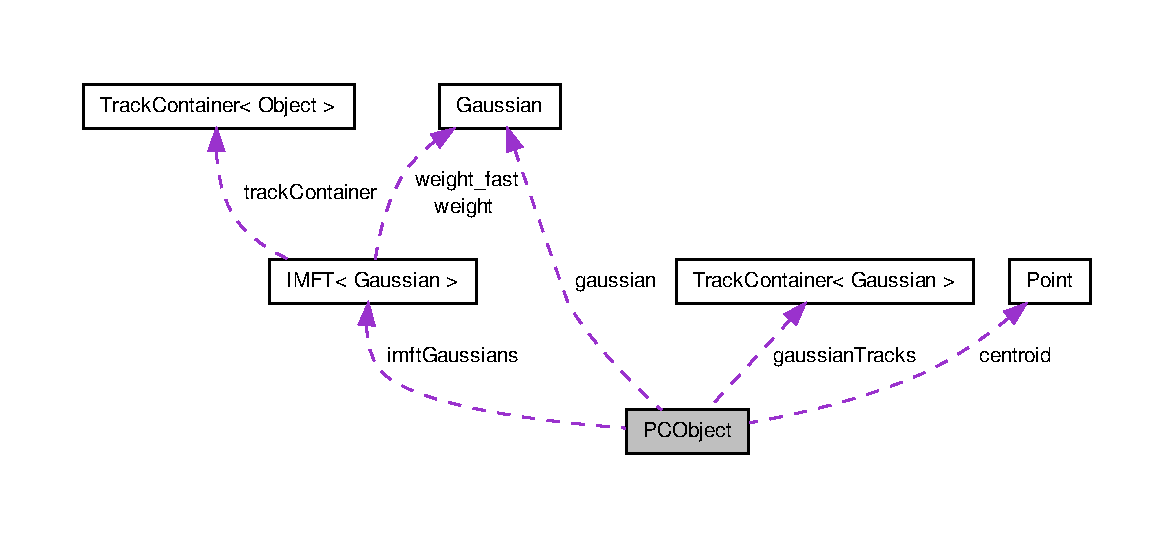
\includegraphics[width=350pt]{class_p_c_object__coll__graph}
\end{center}
\end{figure}
\subsection*{\-Classes}
\begin{DoxyCompactItemize}
\item 
struct \hyperlink{struct_p_c_object_1_1_edge}{\-Edge}
\item 
struct \hyperlink{struct_p_c_object_1_1_edge__spatial}{\-Edge\-\_\-spatial}
\end{DoxyCompactItemize}
\subsection*{\-Public \-Types}
\begin{DoxyCompactItemize}
\item 
typedef double($\ast$ \hyperlink{class_p_c_object_a57717df0ff6fbc92e693c08485479da3}{func\-Weight\-Gaussian} )(\hyperlink{class_gaussian}{\-Gaussian} \&g1, \hyperlink{class_gaussian}{\-Gaussian} \&g2)
\end{DoxyCompactItemize}
\subsection*{\-Public \-Member \-Functions}
\begin{DoxyCompactItemize}
\item 
\hyperlink{class_p_c_object_aad6caa1808cb593e46ff8cbf87c3a29a}{\-P\-C\-Object} ()
\item 
\hyperlink{class_p_c_object_ab5af2877120e54f89d4c4212b2285488}{\-P\-C\-Object} (int \-\_\-id)
\item 
\hyperlink{class_p_c_object_a51c8555367f90194d4c5cbfcd589e812}{$\sim$\-P\-C\-Object} ()
\item 
\hyperlink{common_8h_a36884aa4a3c181fa4c284d79329ad166}{\-Cloud\-Ptr} \hyperlink{class_p_c_object_ae1207c2fc7b1c91274287622c879e56a}{to\-Point\-Cloud} ()
\item 
void \hyperlink{class_p_c_object_ac8872c933f6ebf08abfd1aa4ebde6ebd}{insert} (\hyperlink{class_point}{\-Point} p)
\item 
\hyperlink{class_point}{\-Point} \hyperlink{class_p_c_object_a45a4d281641c441467c976bc390379af}{get\-Centroid} ()
\item 
void \hyperlink{class_p_c_object_a60989cacede56624284ad05f74df9c2a}{initial\-G\-M\-M} (double \-\_\-scale, double \-\_\-percent)
\item 
void \hyperlink{class_p_c_object_a20b15832e2475a1a14e47763a4960109}{filtering\-G\-M\-M\-\_\-\-E\-M} (\hyperlink{class_p_c_object}{\-P\-C\-Object} $\ast$prior)
\item 
void \hyperlink{class_p_c_object_ad85cb4f948c94eb35117fffe54b8d688}{filtering\-G\-M\-M\-\_\-incremental\-E\-M} (\hyperlink{class_p_c_object}{\-P\-C\-Object} $\ast$prior, double \hyperlink{class_p_c_object_a4ac23bed170d9a2993524e4b742c99a4}{percent})
\item 
double \hyperlink{class_p_c_object_a11cc868dc9f8712917148437dc026c57}{likelihood} (\hyperlink{class_point}{\-Point} point, \hyperlink{class_gaussian}{\-Gaussian} \hyperlink{class_p_c_object_a2a0a0fe603bac2c80a43d4f6e224bf98}{gaussian})
\item 
double \hyperlink{class_p_c_object_a2b88860d97b5c8f7b784427ce5a6f5b4}{likelihood\-\_\-standard} (\hyperlink{class_point}{\-Point} point, \hyperlink{class_gaussian}{\-Gaussian} \hyperlink{class_p_c_object_a2a0a0fe603bac2c80a43d4f6e224bf98}{gaussian})
\item 
void \hyperlink{class_p_c_object_adcf48887575738fff69b7e765529520a}{init\-Gaussian} (int dim)
\item 
double \hyperlink{class_p_c_object_a265bc3d88852829822e2954cd7453651}{eval\-G\-M\-M} (\hyperlink{class_point}{\-Point} x)
\item 
double \hyperlink{class_p_c_object_ad64e95414d9c60db29986e4408d64278}{eval\-Closest\-G\-M\-M} (\hyperlink{class_point}{\-Point} x)
\item 
double \hyperlink{class_p_c_object_ae9982821fa0ba9e4f3ae4566dcf535f1}{eval\-Normed\-G\-M\-M} (\hyperlink{class_point}{\-Point} x, double den)
\item 
double \hyperlink{class_p_c_object_a03ee69cf00009002b2868fb91b697116}{eval\-Closest\-Normed\-G\-M\-M} (\hyperlink{class_point}{\-Point} x, double den)
\item 
void \hyperlink{class_p_c_object_a50ee001efcde0b94846e8fbcf8302fb6}{simplify} (int dim, \hyperlink{pcobject_8h_a41767bf2343b5367995c795ada4b6946}{\-S\-I\-M\-P\-L\-E} method, double ratio, int n\-Cluster=0)
\item 
void \hyperlink{class_p_c_object_aad9af1a35617123738d53e1abc80980b}{set\-Trans\-Param} (vnl\-\_\-vector$<$ double $>$ param)
\item 
void \hyperlink{class_p_c_object_a2d282f88c1e9412c7e73cad48690a439}{merge\-Two\-G\-M\-Ms} (\hyperlink{class_p_c_object}{\-P\-C\-Object} $\ast$gmm1, \hyperlink{class_p_c_object}{\-P\-C\-Object} $\ast$gmm2)
\item 
void \hyperlink{class_p_c_object_a3a765ed1df3f4997c7255da3bd53ad6f}{set\-Scale} (double \-\_\-scale)
\item 
void \hyperlink{class_p_c_object_ac085f8a5dc44cfa8f4e4d2d1a9aeacd5}{gaussian\-Tracking\-Init} (int \-\_\-window\-\_\-short, int \-\_\-window\-\_\-long, int \-\_\-max\-I\-D, \hyperlink{class_p_c_object_a57717df0ff6fbc92e693c08485479da3}{func\-Weight\-Gaussian} \-\_\-weight\-\_\-gaussian, \hyperlink{class_p_c_object_a57717df0ff6fbc92e693c08485479da3}{func\-Weight\-Gaussian} \-\_\-weight\-\_\-gaussian\-\_\-fast)
\item 
void \hyperlink{class_p_c_object_a0631fbfafe8050f758c14f0b3791fa01}{gaussian\-Tracking} ()
\item 
void \hyperlink{class_p_c_object_ae117d9276dd14490027029e8b87e150f}{update\-Predictive\-Parameters} ()
\item 
void \hyperlink{class_p_c_object_acfdd2146d888b9d30e7fde9ea6a0727e}{calculate\-Velocity} ()
\item 
void \hyperlink{class_p_c_object_ad14e7453287b842ce8dced26c63d2899}{make\-Topology} ()
\item 
double \hyperlink{class_p_c_object_ae3eaf96866c11430868e643d7fa56eb9}{topology\-\_\-weight} (\hyperlink{class_gaussian}{\-Gaussian} g1, \hyperlink{class_gaussian}{\-Gaussian} g2)
\item 
double \hyperlink{class_p_c_object_a81bcc4f7794825ea6fe97c716e7d751e}{topology\-\_\-posweight\-\_\-rev} (\hyperlink{class_gaussian}{\-Gaussian} g1, \hyperlink{class_gaussian}{\-Gaussian} g2)
\item 
double \hyperlink{class_p_c_object_ae6714b4bc945ea46de699bba08e077b2}{topology\-\_\-velweight\-\_\-rev} (\hyperlink{class_gaussian}{\-Gaussian} g1, \hyperlink{class_gaussian}{\-Gaussian} g2)
\item 
int \hyperlink{class_p_c_object_a12dd695b331e394b56f54920c1b93972}{component\-Graph} (vector$<$ \hyperlink{class_p_c_object}{\-P\-C\-Object} $>$ \&new\-Objects)
\item 
void \hyperlink{class_p_c_object_a0f9cc4c246bd5dc449ba900ef203d82e}{setid} (int \-\_\-id)
\item 
int \hyperlink{class_p_c_object_ab5c524d8bf9e73ec56f5d848b026a13e}{getid} ()
\end{DoxyCompactItemize}
\subsection*{\-Public \-Attributes}
\begin{DoxyCompactItemize}
\item 
vector$<$ \hyperlink{class_point}{\-Point} $>$ \hyperlink{class_p_c_object_a88519afe57e934c37b87cd74201573ae}{points}
\item 
vector$<$ \hyperlink{class_gaussian}{\-Gaussian} $>$ \hyperlink{class_p_c_object_a7eae3d72d8dfedee042050dc80df4423}{gmm}
\item 
\hyperlink{class_point}{\-Point} \hyperlink{class_p_c_object_a827d54b95fd8fbe64bd4f0fe7a7c1c80}{centroid}
\item 
\hyperlink{class_gaussian}{\-Gaussian} \hyperlink{class_p_c_object_a2a0a0fe603bac2c80a43d4f6e224bf98}{gaussian}
\item 
\hyperlink{pcobject_8h_a275a67132f10277ada3a0ee3d616b647}{\-S\-T\-A\-T\-E} \hyperlink{class_p_c_object_ad5a0566f1118a4e70d1de788c7dd4c06}{state}
\item 
int \hyperlink{class_p_c_object_aec75ff9931a685504afff6a7c1f78c02}{dimension}
\item 
int \hyperlink{class_p_c_object_a57cb1270dee62f9c65643f3cbe03347e}{id}
\item 
vnl\-\_\-vector$<$ double $>$ \hyperlink{class_p_c_object_aca5e8c66727c01980551ac8744bfb26a}{trans\-\_\-param}
\item 
bool \hyperlink{class_p_c_object_ab9a8f0b1f9d3b4851877e15e17582097}{is\-Param\-Exist}
\item 
\hyperlink{class_i_m_f_t}{\-I\-M\-F\-T}$<$ \hyperlink{class_gaussian}{\-Gaussian} $>$ $\ast$ \hyperlink{class_p_c_object_aa921fc68268138b7f5026ec1ccaef619}{imft\-Gaussians}
\item 
\hyperlink{class_track_container}{\-Track\-Container}$<$ \hyperlink{class_gaussian}{\-Gaussian} $>$ $\ast$ \hyperlink{class_p_c_object_a7d7a327eda5d75b554e2c83ba32a8517}{gaussian\-Tracks}
\item 
int \hyperlink{class_p_c_object_a1e854b1f05424e21b57571c4d5d3a639}{cnt}
\item 
vector$<$ \hyperlink{class_gaussian}{\-Gaussian} $\ast$ $>$ \hyperlink{class_p_c_object_acbc764cefd102f6b184192ffa266510f}{frame}
\item 
\-List\-Graph $\ast$ \hyperlink{class_p_c_object_a1e2497e50fb2af6cf043d91b3d2e14c6}{topology\-\_\-graph}
\item 
\-List\-Graph\-::\-Node\-Map$<$ \hyperlink{class_gaussian}{\-Gaussian} $>$ $\ast$ \hyperlink{class_p_c_object_a99eafcc86b98ec0f1d165b8a96d351dc}{topology\-\_\-node\-Map}
\item 
\-List\-Graph\-::\-Edge\-Map$<$ double $>$ $\ast$ \hyperlink{class_p_c_object_a5f09a7006b5499186fe9908143dfbee9}{topology\-\_\-edge\-Map}
\item 
vector$<$ \hyperlink{struct_p_c_object_1_1_edge}{\-Edge} $>$ \hyperlink{class_p_c_object_a0d6dab1fe4edd99095e1fe236d4910a5}{edges}
\item 
double \hyperlink{class_p_c_object_ac94a79d35dece547fab98be2b70e9604}{alpha}
\item 
double \hyperlink{class_p_c_object_a2e2e26d46ec23849c062e9d28d349778}{th\-\_\-edge}
\item 
double $\ast$ \hyperlink{class_p_c_object_ae08580ed200d25aa8304fde6f924c9f3}{diff\-Weight}
\item 
double \hyperlink{class_p_c_object_a959539770a6c61a3db3ef480140d1ed0}{filtered\-Weight}
\item 
double \hyperlink{class_p_c_object_a8737196626b96a2730810a9cee2330ed}{scale}
\item 
double \hyperlink{class_p_c_object_a4ac23bed170d9a2993524e4b742c99a4}{percent}
\end{DoxyCompactItemize}
\subsection*{\-Private \-Attributes}
\begin{DoxyCompactItemize}
\item 
int \hyperlink{class_p_c_object_a6c90b358d6d19ab437841f829e448b7c}{window\-\_\-short}
\item 
int \hyperlink{class_p_c_object_a1606ff67b8422eac1ee46849bffdb69a}{window\-\_\-long}
\end{DoxyCompactItemize}


\subsection{\-Member \-Typedef \-Documentation}
\hypertarget{class_p_c_object_a57717df0ff6fbc92e693c08485479da3}{\index{\-P\-C\-Object@{\-P\-C\-Object}!func\-Weight\-Gaussian@{func\-Weight\-Gaussian}}
\index{func\-Weight\-Gaussian@{func\-Weight\-Gaussian}!PCObject@{\-P\-C\-Object}}
\subsubsection[{func\-Weight\-Gaussian}]{\setlength{\rightskip}{0pt plus 5cm}typedef double($\ast$ {\bf \-P\-C\-Object\-::func\-Weight\-Gaussian})({\bf \-Gaussian} \&g1, {\bf \-Gaussian} \&g2)}}\label{class_p_c_object_a57717df0ff6fbc92e693c08485479da3}


\subsection{\-Constructor \& \-Destructor \-Documentation}
\hypertarget{class_p_c_object_aad6caa1808cb593e46ff8cbf87c3a29a}{\index{\-P\-C\-Object@{\-P\-C\-Object}!\-P\-C\-Object@{\-P\-C\-Object}}
\index{\-P\-C\-Object@{\-P\-C\-Object}!PCObject@{\-P\-C\-Object}}
\subsubsection[{\-P\-C\-Object}]{\setlength{\rightskip}{0pt plus 5cm}{\bf \-P\-C\-Object\-::\-P\-C\-Object} (
\begin{DoxyParamCaption}
{}
\end{DoxyParamCaption}
)}}\label{class_p_c_object_aad6caa1808cb593e46ff8cbf87c3a29a}
\hypertarget{class_p_c_object_ab5af2877120e54f89d4c4212b2285488}{\index{\-P\-C\-Object@{\-P\-C\-Object}!\-P\-C\-Object@{\-P\-C\-Object}}
\index{\-P\-C\-Object@{\-P\-C\-Object}!PCObject@{\-P\-C\-Object}}
\subsubsection[{\-P\-C\-Object}]{\setlength{\rightskip}{0pt plus 5cm}{\bf \-P\-C\-Object\-::\-P\-C\-Object} (
\begin{DoxyParamCaption}
\item[{int}]{\-\_\-id}
\end{DoxyParamCaption}
)}}\label{class_p_c_object_ab5af2877120e54f89d4c4212b2285488}
\hypertarget{class_p_c_object_a51c8555367f90194d4c5cbfcd589e812}{\index{\-P\-C\-Object@{\-P\-C\-Object}!$\sim$\-P\-C\-Object@{$\sim$\-P\-C\-Object}}
\index{$\sim$\-P\-C\-Object@{$\sim$\-P\-C\-Object}!PCObject@{\-P\-C\-Object}}
\subsubsection[{$\sim$\-P\-C\-Object}]{\setlength{\rightskip}{0pt plus 5cm}{\bf \-P\-C\-Object\-::$\sim$\-P\-C\-Object} (
\begin{DoxyParamCaption}
{}
\end{DoxyParamCaption}
)}}\label{class_p_c_object_a51c8555367f90194d4c5cbfcd589e812}


\subsection{\-Member \-Function \-Documentation}
\hypertarget{class_p_c_object_acfdd2146d888b9d30e7fde9ea6a0727e}{\index{\-P\-C\-Object@{\-P\-C\-Object}!calculate\-Velocity@{calculate\-Velocity}}
\index{calculate\-Velocity@{calculate\-Velocity}!PCObject@{\-P\-C\-Object}}
\subsubsection[{calculate\-Velocity}]{\setlength{\rightskip}{0pt plus 5cm}void {\bf \-P\-C\-Object\-::calculate\-Velocity} (
\begin{DoxyParamCaption}
{}
\end{DoxyParamCaption}
)}}\label{class_p_c_object_acfdd2146d888b9d30e7fde9ea6a0727e}


\-Here is the call graph for this function\-:
\nopagebreak
\begin{figure}[H]
\begin{center}
\leavevmode
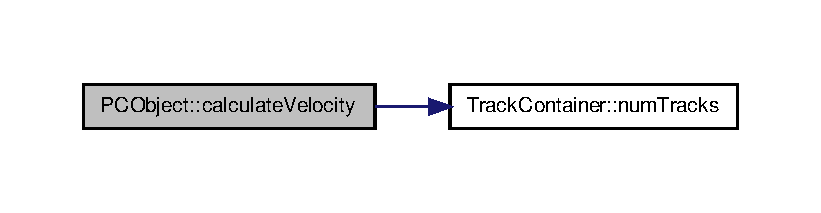
\includegraphics[width=350pt]{class_p_c_object_acfdd2146d888b9d30e7fde9ea6a0727e_cgraph}
\end{center}
\end{figure}


\hypertarget{class_p_c_object_a12dd695b331e394b56f54920c1b93972}{\index{\-P\-C\-Object@{\-P\-C\-Object}!component\-Graph@{component\-Graph}}
\index{component\-Graph@{component\-Graph}!PCObject@{\-P\-C\-Object}}
\subsubsection[{component\-Graph}]{\setlength{\rightskip}{0pt plus 5cm}int {\bf \-P\-C\-Object\-::component\-Graph} (
\begin{DoxyParamCaption}
\item[{vector$<$ {\bf \-P\-C\-Object} $>$ \&}]{new\-Objects}
\end{DoxyParamCaption}
)}}\label{class_p_c_object_a12dd695b331e394b56f54920c1b93972}
\hypertarget{class_p_c_object_ad64e95414d9c60db29986e4408d64278}{\index{\-P\-C\-Object@{\-P\-C\-Object}!eval\-Closest\-G\-M\-M@{eval\-Closest\-G\-M\-M}}
\index{eval\-Closest\-G\-M\-M@{eval\-Closest\-G\-M\-M}!PCObject@{\-P\-C\-Object}}
\subsubsection[{eval\-Closest\-G\-M\-M}]{\setlength{\rightskip}{0pt plus 5cm}double {\bf \-P\-C\-Object\-::eval\-Closest\-G\-M\-M} (
\begin{DoxyParamCaption}
\item[{{\bf \-Point}}]{x}
\end{DoxyParamCaption}
)}}\label{class_p_c_object_ad64e95414d9c60db29986e4408d64278}
\hypertarget{class_p_c_object_a03ee69cf00009002b2868fb91b697116}{\index{\-P\-C\-Object@{\-P\-C\-Object}!eval\-Closest\-Normed\-G\-M\-M@{eval\-Closest\-Normed\-G\-M\-M}}
\index{eval\-Closest\-Normed\-G\-M\-M@{eval\-Closest\-Normed\-G\-M\-M}!PCObject@{\-P\-C\-Object}}
\subsubsection[{eval\-Closest\-Normed\-G\-M\-M}]{\setlength{\rightskip}{0pt plus 5cm}double {\bf \-P\-C\-Object\-::eval\-Closest\-Normed\-G\-M\-M} (
\begin{DoxyParamCaption}
\item[{{\bf \-Point}}]{x, }
\item[{double}]{den}
\end{DoxyParamCaption}
)}}\label{class_p_c_object_a03ee69cf00009002b2868fb91b697116}
\hypertarget{class_p_c_object_a265bc3d88852829822e2954cd7453651}{\index{\-P\-C\-Object@{\-P\-C\-Object}!eval\-G\-M\-M@{eval\-G\-M\-M}}
\index{eval\-G\-M\-M@{eval\-G\-M\-M}!PCObject@{\-P\-C\-Object}}
\subsubsection[{eval\-G\-M\-M}]{\setlength{\rightskip}{0pt plus 5cm}double {\bf \-P\-C\-Object\-::eval\-G\-M\-M} (
\begin{DoxyParamCaption}
\item[{{\bf \-Point}}]{x}
\end{DoxyParamCaption}
)}}\label{class_p_c_object_a265bc3d88852829822e2954cd7453651}
\hypertarget{class_p_c_object_ae9982821fa0ba9e4f3ae4566dcf535f1}{\index{\-P\-C\-Object@{\-P\-C\-Object}!eval\-Normed\-G\-M\-M@{eval\-Normed\-G\-M\-M}}
\index{eval\-Normed\-G\-M\-M@{eval\-Normed\-G\-M\-M}!PCObject@{\-P\-C\-Object}}
\subsubsection[{eval\-Normed\-G\-M\-M}]{\setlength{\rightskip}{0pt plus 5cm}double {\bf \-P\-C\-Object\-::eval\-Normed\-G\-M\-M} (
\begin{DoxyParamCaption}
\item[{{\bf \-Point}}]{x, }
\item[{double}]{den}
\end{DoxyParamCaption}
)}}\label{class_p_c_object_ae9982821fa0ba9e4f3ae4566dcf535f1}
\hypertarget{class_p_c_object_a20b15832e2475a1a14e47763a4960109}{\index{\-P\-C\-Object@{\-P\-C\-Object}!filtering\-G\-M\-M\-\_\-\-E\-M@{filtering\-G\-M\-M\-\_\-\-E\-M}}
\index{filtering\-G\-M\-M\-\_\-\-E\-M@{filtering\-G\-M\-M\-\_\-\-E\-M}!PCObject@{\-P\-C\-Object}}
\subsubsection[{filtering\-G\-M\-M\-\_\-\-E\-M}]{\setlength{\rightskip}{0pt plus 5cm}void {\bf \-P\-C\-Object\-::filtering\-G\-M\-M\-\_\-\-E\-M} (
\begin{DoxyParamCaption}
\item[{{\bf \-P\-C\-Object} $\ast$}]{prior}
\end{DoxyParamCaption}
)}}\label{class_p_c_object_a20b15832e2475a1a14e47763a4960109}


\-Here is the call graph for this function\-:
\nopagebreak
\begin{figure}[H]
\begin{center}
\leavevmode
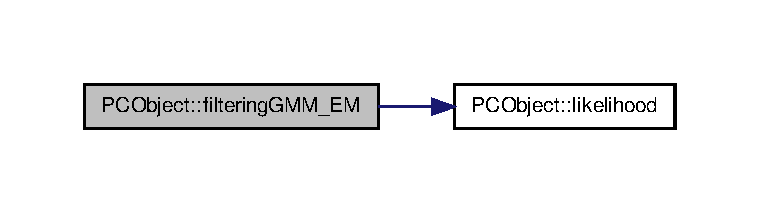
\includegraphics[width=350pt]{class_p_c_object_a20b15832e2475a1a14e47763a4960109_cgraph}
\end{center}
\end{figure}


\hypertarget{class_p_c_object_ad85cb4f948c94eb35117fffe54b8d688}{\index{\-P\-C\-Object@{\-P\-C\-Object}!filtering\-G\-M\-M\-\_\-incremental\-E\-M@{filtering\-G\-M\-M\-\_\-incremental\-E\-M}}
\index{filtering\-G\-M\-M\-\_\-incremental\-E\-M@{filtering\-G\-M\-M\-\_\-incremental\-E\-M}!PCObject@{\-P\-C\-Object}}
\subsubsection[{filtering\-G\-M\-M\-\_\-incremental\-E\-M}]{\setlength{\rightskip}{0pt plus 5cm}void {\bf \-P\-C\-Object\-::filtering\-G\-M\-M\-\_\-incremental\-E\-M} (
\begin{DoxyParamCaption}
\item[{{\bf \-P\-C\-Object} $\ast$}]{prior, }
\item[{double}]{percent}
\end{DoxyParamCaption}
)}}\label{class_p_c_object_ad85cb4f948c94eb35117fffe54b8d688}


\-Here is the call graph for this function\-:
\nopagebreak
\begin{figure}[H]
\begin{center}
\leavevmode
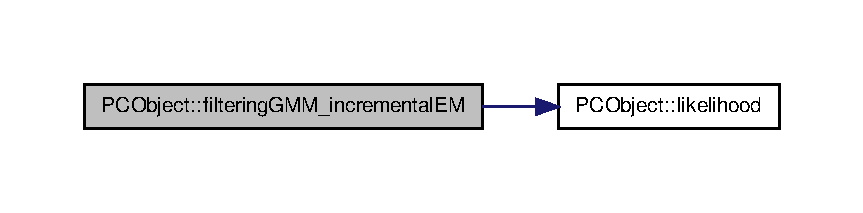
\includegraphics[width=350pt]{class_p_c_object_ad85cb4f948c94eb35117fffe54b8d688_cgraph}
\end{center}
\end{figure}


\hypertarget{class_p_c_object_a0631fbfafe8050f758c14f0b3791fa01}{\index{\-P\-C\-Object@{\-P\-C\-Object}!gaussian\-Tracking@{gaussian\-Tracking}}
\index{gaussian\-Tracking@{gaussian\-Tracking}!PCObject@{\-P\-C\-Object}}
\subsubsection[{gaussian\-Tracking}]{\setlength{\rightskip}{0pt plus 5cm}void {\bf \-P\-C\-Object\-::gaussian\-Tracking} (
\begin{DoxyParamCaption}
{}
\end{DoxyParamCaption}
)}}\label{class_p_c_object_a0631fbfafe8050f758c14f0b3791fa01}


\-Here is the call graph for this function\-:
\nopagebreak
\begin{figure}[H]
\begin{center}
\leavevmode
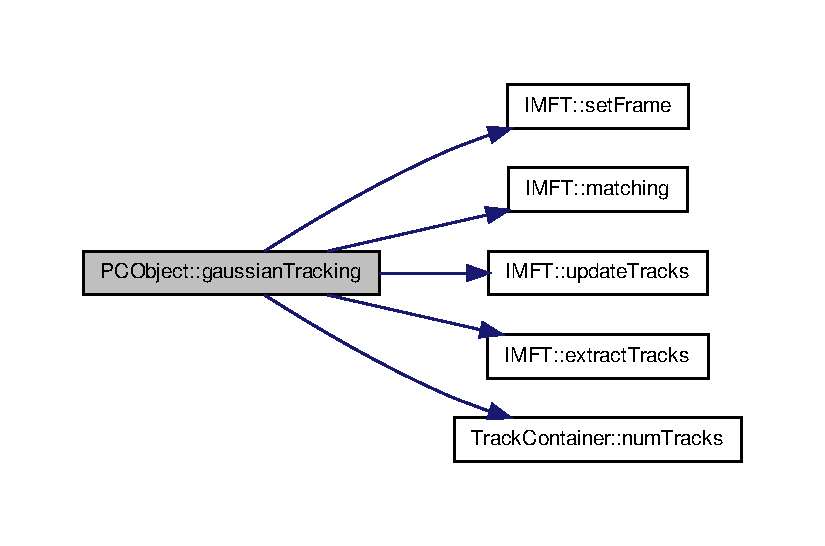
\includegraphics[width=350pt]{class_p_c_object_a0631fbfafe8050f758c14f0b3791fa01_cgraph}
\end{center}
\end{figure}


\hypertarget{class_p_c_object_ac085f8a5dc44cfa8f4e4d2d1a9aeacd5}{\index{\-P\-C\-Object@{\-P\-C\-Object}!gaussian\-Tracking\-Init@{gaussian\-Tracking\-Init}}
\index{gaussian\-Tracking\-Init@{gaussian\-Tracking\-Init}!PCObject@{\-P\-C\-Object}}
\subsubsection[{gaussian\-Tracking\-Init}]{\setlength{\rightskip}{0pt plus 5cm}void {\bf \-P\-C\-Object\-::gaussian\-Tracking\-Init} (
\begin{DoxyParamCaption}
\item[{int}]{\-\_\-window\-\_\-short, }
\item[{int}]{\-\_\-window\-\_\-long, }
\item[{int}]{\-\_\-max\-I\-D, }
\item[{{\bf func\-Weight\-Gaussian}}]{\-\_\-weight\-\_\-gaussian, }
\item[{{\bf func\-Weight\-Gaussian}}]{\-\_\-weight\-\_\-gaussian\-\_\-fast}
\end{DoxyParamCaption}
)}}\label{class_p_c_object_ac085f8a5dc44cfa8f4e4d2d1a9aeacd5}


\-Here is the call graph for this function\-:
\nopagebreak
\begin{figure}[H]
\begin{center}
\leavevmode
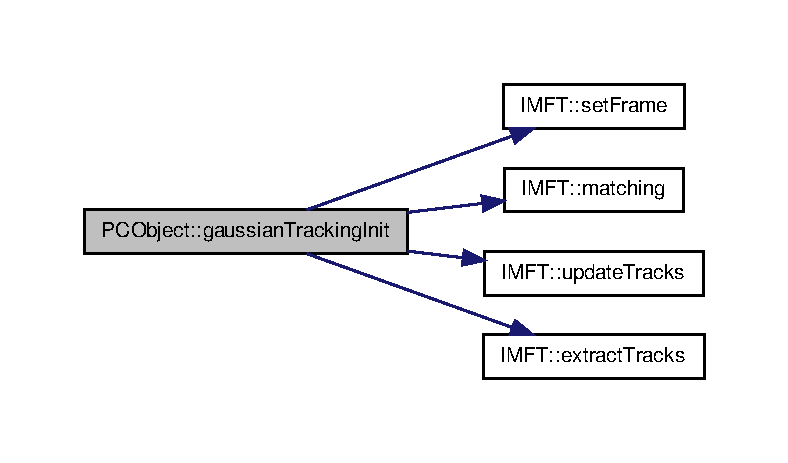
\includegraphics[width=350pt]{class_p_c_object_ac085f8a5dc44cfa8f4e4d2d1a9aeacd5_cgraph}
\end{center}
\end{figure}


\hypertarget{class_p_c_object_a45a4d281641c441467c976bc390379af}{\index{\-P\-C\-Object@{\-P\-C\-Object}!get\-Centroid@{get\-Centroid}}
\index{get\-Centroid@{get\-Centroid}!PCObject@{\-P\-C\-Object}}
\subsubsection[{get\-Centroid}]{\setlength{\rightskip}{0pt plus 5cm}{\bf \-Point} {\bf \-P\-C\-Object\-::get\-Centroid} (
\begin{DoxyParamCaption}
{}
\end{DoxyParamCaption}
)}}\label{class_p_c_object_a45a4d281641c441467c976bc390379af}
\hypertarget{class_p_c_object_ab5c524d8bf9e73ec56f5d848b026a13e}{\index{\-P\-C\-Object@{\-P\-C\-Object}!getid@{getid}}
\index{getid@{getid}!PCObject@{\-P\-C\-Object}}
\subsubsection[{getid}]{\setlength{\rightskip}{0pt plus 5cm}int {\bf \-P\-C\-Object\-::getid} (
\begin{DoxyParamCaption}
{}
\end{DoxyParamCaption}
)\hspace{0.3cm}{\ttfamily  \mbox{[}inline\mbox{]}}}}\label{class_p_c_object_ab5c524d8bf9e73ec56f5d848b026a13e}
\hypertarget{class_p_c_object_adcf48887575738fff69b7e765529520a}{\index{\-P\-C\-Object@{\-P\-C\-Object}!init\-Gaussian@{init\-Gaussian}}
\index{init\-Gaussian@{init\-Gaussian}!PCObject@{\-P\-C\-Object}}
\subsubsection[{init\-Gaussian}]{\setlength{\rightskip}{0pt plus 5cm}void {\bf \-P\-C\-Object\-::init\-Gaussian} (
\begin{DoxyParamCaption}
\item[{int}]{dim}
\end{DoxyParamCaption}
)}}\label{class_p_c_object_adcf48887575738fff69b7e765529520a}


\-Here is the call graph for this function\-:
\nopagebreak
\begin{figure}[H]
\begin{center}
\leavevmode
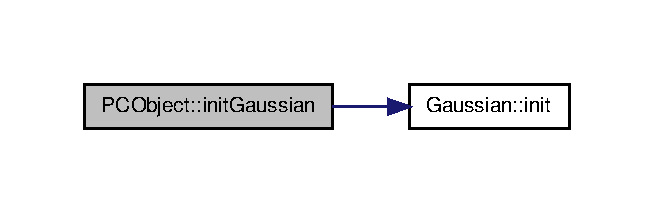
\includegraphics[width=314pt]{class_p_c_object_adcf48887575738fff69b7e765529520a_cgraph}
\end{center}
\end{figure}




\-Here is the caller graph for this function\-:
\nopagebreak
\begin{figure}[H]
\begin{center}
\leavevmode
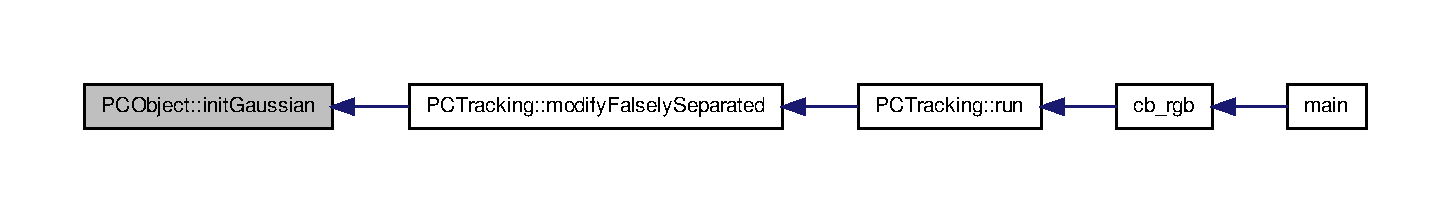
\includegraphics[width=350pt]{class_p_c_object_adcf48887575738fff69b7e765529520a_icgraph}
\end{center}
\end{figure}


\hypertarget{class_p_c_object_a60989cacede56624284ad05f74df9c2a}{\index{\-P\-C\-Object@{\-P\-C\-Object}!initial\-G\-M\-M@{initial\-G\-M\-M}}
\index{initial\-G\-M\-M@{initial\-G\-M\-M}!PCObject@{\-P\-C\-Object}}
\subsubsection[{initial\-G\-M\-M}]{\setlength{\rightskip}{0pt plus 5cm}void {\bf \-P\-C\-Object\-::initial\-G\-M\-M} (
\begin{DoxyParamCaption}
\item[{double}]{\-\_\-scale, }
\item[{double}]{\-\_\-percent}
\end{DoxyParamCaption}
)}}\label{class_p_c_object_a60989cacede56624284ad05f74df9c2a}


\-Here is the call graph for this function\-:
\nopagebreak
\begin{figure}[H]
\begin{center}
\leavevmode
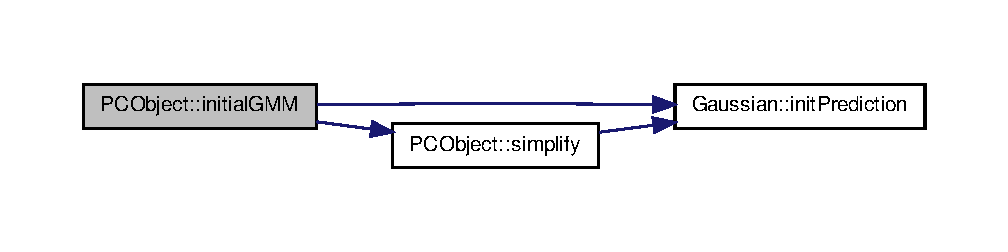
\includegraphics[width=350pt]{class_p_c_object_a60989cacede56624284ad05f74df9c2a_cgraph}
\end{center}
\end{figure}


\hypertarget{class_p_c_object_ac8872c933f6ebf08abfd1aa4ebde6ebd}{\index{\-P\-C\-Object@{\-P\-C\-Object}!insert@{insert}}
\index{insert@{insert}!PCObject@{\-P\-C\-Object}}
\subsubsection[{insert}]{\setlength{\rightskip}{0pt plus 5cm}void {\bf \-P\-C\-Object\-::insert} (
\begin{DoxyParamCaption}
\item[{{\bf \-Point}}]{p}
\end{DoxyParamCaption}
)}}\label{class_p_c_object_ac8872c933f6ebf08abfd1aa4ebde6ebd}


\-Here is the caller graph for this function\-:
\nopagebreak
\begin{figure}[H]
\begin{center}
\leavevmode
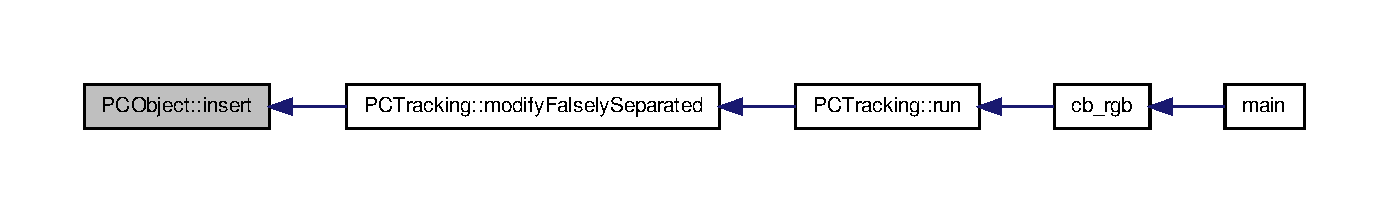
\includegraphics[width=350pt]{class_p_c_object_ac8872c933f6ebf08abfd1aa4ebde6ebd_icgraph}
\end{center}
\end{figure}


\hypertarget{class_p_c_object_a11cc868dc9f8712917148437dc026c57}{\index{\-P\-C\-Object@{\-P\-C\-Object}!likelihood@{likelihood}}
\index{likelihood@{likelihood}!PCObject@{\-P\-C\-Object}}
\subsubsection[{likelihood}]{\setlength{\rightskip}{0pt plus 5cm}double {\bf \-P\-C\-Object\-::likelihood} (
\begin{DoxyParamCaption}
\item[{{\bf \-Point}}]{point, }
\item[{{\bf \-Gaussian}}]{gaussian}
\end{DoxyParamCaption}
)}}\label{class_p_c_object_a11cc868dc9f8712917148437dc026c57}


\-Here is the caller graph for this function\-:
\nopagebreak
\begin{figure}[H]
\begin{center}
\leavevmode
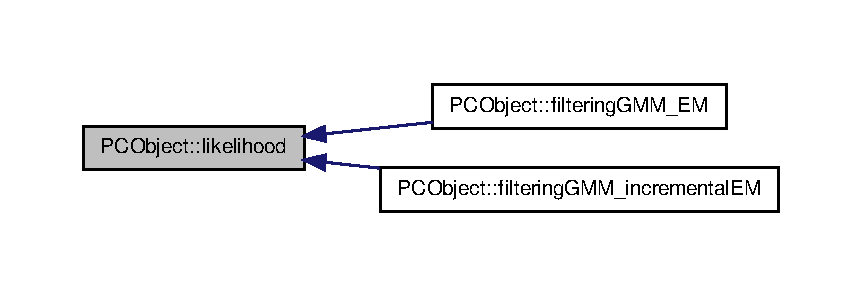
\includegraphics[width=350pt]{class_p_c_object_a11cc868dc9f8712917148437dc026c57_icgraph}
\end{center}
\end{figure}


\hypertarget{class_p_c_object_a2b88860d97b5c8f7b784427ce5a6f5b4}{\index{\-P\-C\-Object@{\-P\-C\-Object}!likelihood\-\_\-standard@{likelihood\-\_\-standard}}
\index{likelihood\-\_\-standard@{likelihood\-\_\-standard}!PCObject@{\-P\-C\-Object}}
\subsubsection[{likelihood\-\_\-standard}]{\setlength{\rightskip}{0pt plus 5cm}double {\bf \-P\-C\-Object\-::likelihood\-\_\-standard} (
\begin{DoxyParamCaption}
\item[{{\bf \-Point}}]{point, }
\item[{{\bf \-Gaussian}}]{gaussian}
\end{DoxyParamCaption}
)}}\label{class_p_c_object_a2b88860d97b5c8f7b784427ce5a6f5b4}
\hypertarget{class_p_c_object_ad14e7453287b842ce8dced26c63d2899}{\index{\-P\-C\-Object@{\-P\-C\-Object}!make\-Topology@{make\-Topology}}
\index{make\-Topology@{make\-Topology}!PCObject@{\-P\-C\-Object}}
\subsubsection[{make\-Topology}]{\setlength{\rightskip}{0pt plus 5cm}void {\bf \-P\-C\-Object\-::make\-Topology} (
\begin{DoxyParamCaption}
{}
\end{DoxyParamCaption}
)}}\label{class_p_c_object_ad14e7453287b842ce8dced26c63d2899}


\-Here is the call graph for this function\-:
\nopagebreak
\begin{figure}[H]
\begin{center}
\leavevmode
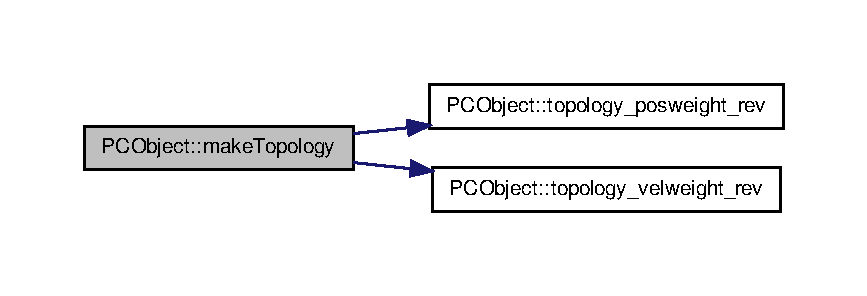
\includegraphics[width=350pt]{class_p_c_object_ad14e7453287b842ce8dced26c63d2899_cgraph}
\end{center}
\end{figure}


\hypertarget{class_p_c_object_a2d282f88c1e9412c7e73cad48690a439}{\index{\-P\-C\-Object@{\-P\-C\-Object}!merge\-Two\-G\-M\-Ms@{merge\-Two\-G\-M\-Ms}}
\index{merge\-Two\-G\-M\-Ms@{merge\-Two\-G\-M\-Ms}!PCObject@{\-P\-C\-Object}}
\subsubsection[{merge\-Two\-G\-M\-Ms}]{\setlength{\rightskip}{0pt plus 5cm}void {\bf \-P\-C\-Object\-::merge\-Two\-G\-M\-Ms} (
\begin{DoxyParamCaption}
\item[{{\bf \-P\-C\-Object} $\ast$}]{gmm1, }
\item[{{\bf \-P\-C\-Object} $\ast$}]{gmm2}
\end{DoxyParamCaption}
)}}\label{class_p_c_object_a2d282f88c1e9412c7e73cad48690a439}
\hypertarget{class_p_c_object_a0f9cc4c246bd5dc449ba900ef203d82e}{\index{\-P\-C\-Object@{\-P\-C\-Object}!setid@{setid}}
\index{setid@{setid}!PCObject@{\-P\-C\-Object}}
\subsubsection[{setid}]{\setlength{\rightskip}{0pt plus 5cm}void {\bf \-P\-C\-Object\-::setid} (
\begin{DoxyParamCaption}
\item[{int}]{\-\_\-id}
\end{DoxyParamCaption}
)\hspace{0.3cm}{\ttfamily  \mbox{[}inline\mbox{]}}}}\label{class_p_c_object_a0f9cc4c246bd5dc449ba900ef203d82e}
\hypertarget{class_p_c_object_a3a765ed1df3f4997c7255da3bd53ad6f}{\index{\-P\-C\-Object@{\-P\-C\-Object}!set\-Scale@{set\-Scale}}
\index{set\-Scale@{set\-Scale}!PCObject@{\-P\-C\-Object}}
\subsubsection[{set\-Scale}]{\setlength{\rightskip}{0pt plus 5cm}void {\bf \-P\-C\-Object\-::set\-Scale} (
\begin{DoxyParamCaption}
\item[{double}]{\-\_\-scale}
\end{DoxyParamCaption}
)\hspace{0.3cm}{\ttfamily  \mbox{[}inline\mbox{]}}}}\label{class_p_c_object_a3a765ed1df3f4997c7255da3bd53ad6f}
\hypertarget{class_p_c_object_aad9af1a35617123738d53e1abc80980b}{\index{\-P\-C\-Object@{\-P\-C\-Object}!set\-Trans\-Param@{set\-Trans\-Param}}
\index{set\-Trans\-Param@{set\-Trans\-Param}!PCObject@{\-P\-C\-Object}}
\subsubsection[{set\-Trans\-Param}]{\setlength{\rightskip}{0pt plus 5cm}void {\bf \-P\-C\-Object\-::set\-Trans\-Param} (
\begin{DoxyParamCaption}
\item[{vnl\-\_\-vector$<$ double $>$}]{param}
\end{DoxyParamCaption}
)}}\label{class_p_c_object_aad9af1a35617123738d53e1abc80980b}
\hypertarget{class_p_c_object_a50ee001efcde0b94846e8fbcf8302fb6}{\index{\-P\-C\-Object@{\-P\-C\-Object}!simplify@{simplify}}
\index{simplify@{simplify}!PCObject@{\-P\-C\-Object}}
\subsubsection[{simplify}]{\setlength{\rightskip}{0pt plus 5cm}void {\bf \-P\-C\-Object\-::simplify} (
\begin{DoxyParamCaption}
\item[{int}]{dim, }
\item[{{\bf \-S\-I\-M\-P\-L\-E}}]{method, }
\item[{double}]{ratio, }
\item[{int}]{n\-Cluster = {\ttfamily 0}}
\end{DoxyParamCaption}
)}}\label{class_p_c_object_a50ee001efcde0b94846e8fbcf8302fb6}


\-Here is the call graph for this function\-:
\nopagebreak
\begin{figure}[H]
\begin{center}
\leavevmode
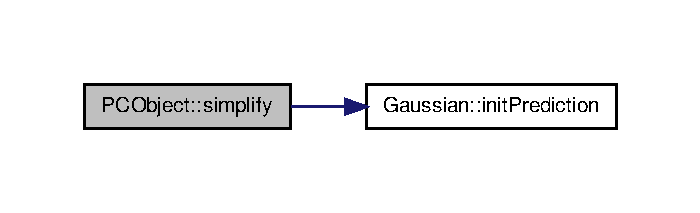
\includegraphics[width=336pt]{class_p_c_object_a50ee001efcde0b94846e8fbcf8302fb6_cgraph}
\end{center}
\end{figure}




\-Here is the caller graph for this function\-:
\nopagebreak
\begin{figure}[H]
\begin{center}
\leavevmode
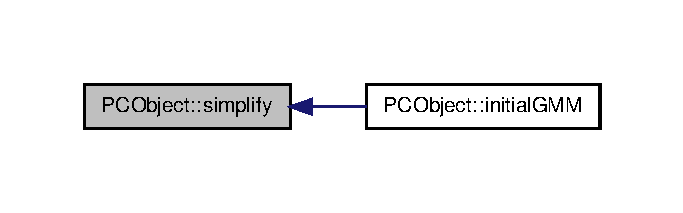
\includegraphics[width=328pt]{class_p_c_object_a50ee001efcde0b94846e8fbcf8302fb6_icgraph}
\end{center}
\end{figure}


\hypertarget{class_p_c_object_ae1207c2fc7b1c91274287622c879e56a}{\index{\-P\-C\-Object@{\-P\-C\-Object}!to\-Point\-Cloud@{to\-Point\-Cloud}}
\index{to\-Point\-Cloud@{to\-Point\-Cloud}!PCObject@{\-P\-C\-Object}}
\subsubsection[{to\-Point\-Cloud}]{\setlength{\rightskip}{0pt plus 5cm}{\bf \-Cloud\-Ptr} {\bf \-P\-C\-Object\-::to\-Point\-Cloud} (
\begin{DoxyParamCaption}
{}
\end{DoxyParamCaption}
)}}\label{class_p_c_object_ae1207c2fc7b1c91274287622c879e56a}


\-Here is the caller graph for this function\-:
\nopagebreak
\begin{figure}[H]
\begin{center}
\leavevmode
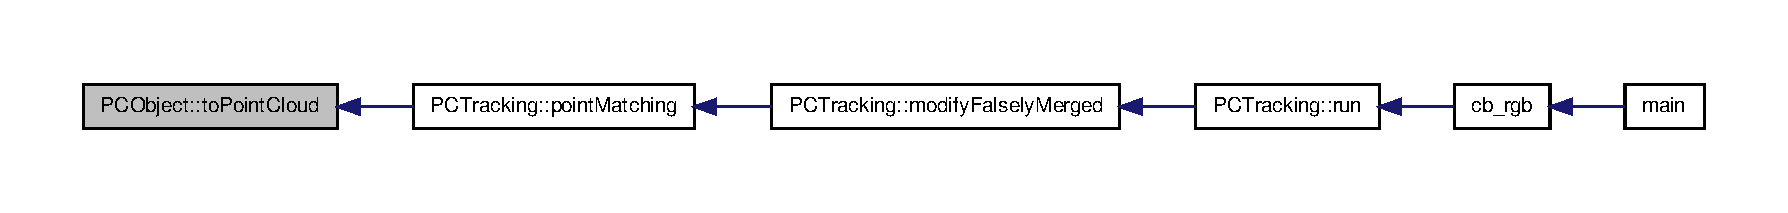
\includegraphics[width=350pt]{class_p_c_object_ae1207c2fc7b1c91274287622c879e56a_icgraph}
\end{center}
\end{figure}


\hypertarget{class_p_c_object_a81bcc4f7794825ea6fe97c716e7d751e}{\index{\-P\-C\-Object@{\-P\-C\-Object}!topology\-\_\-posweight\-\_\-rev@{topology\-\_\-posweight\-\_\-rev}}
\index{topology\-\_\-posweight\-\_\-rev@{topology\-\_\-posweight\-\_\-rev}!PCObject@{\-P\-C\-Object}}
\subsubsection[{topology\-\_\-posweight\-\_\-rev}]{\setlength{\rightskip}{0pt plus 5cm}double {\bf \-P\-C\-Object\-::topology\-\_\-posweight\-\_\-rev} (
\begin{DoxyParamCaption}
\item[{{\bf \-Gaussian}}]{g1, }
\item[{{\bf \-Gaussian}}]{g2}
\end{DoxyParamCaption}
)}}\label{class_p_c_object_a81bcc4f7794825ea6fe97c716e7d751e}


\-Here is the caller graph for this function\-:
\nopagebreak
\begin{figure}[H]
\begin{center}
\leavevmode
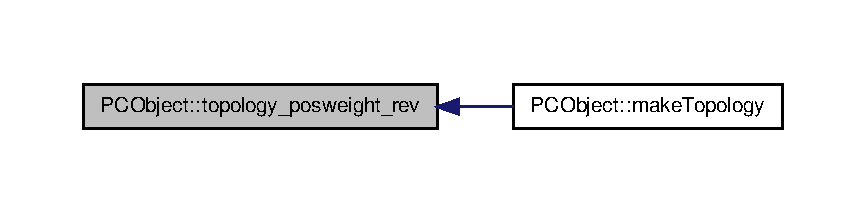
\includegraphics[width=350pt]{class_p_c_object_a81bcc4f7794825ea6fe97c716e7d751e_icgraph}
\end{center}
\end{figure}


\hypertarget{class_p_c_object_ae6714b4bc945ea46de699bba08e077b2}{\index{\-P\-C\-Object@{\-P\-C\-Object}!topology\-\_\-velweight\-\_\-rev@{topology\-\_\-velweight\-\_\-rev}}
\index{topology\-\_\-velweight\-\_\-rev@{topology\-\_\-velweight\-\_\-rev}!PCObject@{\-P\-C\-Object}}
\subsubsection[{topology\-\_\-velweight\-\_\-rev}]{\setlength{\rightskip}{0pt plus 5cm}double {\bf \-P\-C\-Object\-::topology\-\_\-velweight\-\_\-rev} (
\begin{DoxyParamCaption}
\item[{{\bf \-Gaussian}}]{g1, }
\item[{{\bf \-Gaussian}}]{g2}
\end{DoxyParamCaption}
)}}\label{class_p_c_object_ae6714b4bc945ea46de699bba08e077b2}


\-Here is the caller graph for this function\-:
\nopagebreak
\begin{figure}[H]
\begin{center}
\leavevmode
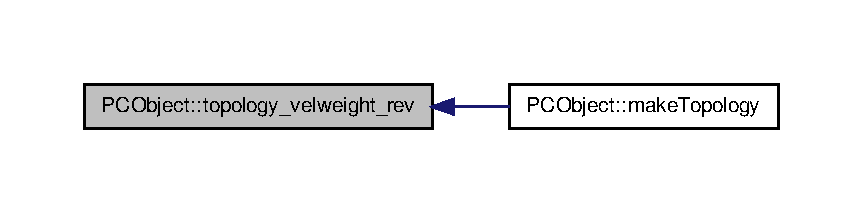
\includegraphics[width=350pt]{class_p_c_object_ae6714b4bc945ea46de699bba08e077b2_icgraph}
\end{center}
\end{figure}


\hypertarget{class_p_c_object_ae3eaf96866c11430868e643d7fa56eb9}{\index{\-P\-C\-Object@{\-P\-C\-Object}!topology\-\_\-weight@{topology\-\_\-weight}}
\index{topology\-\_\-weight@{topology\-\_\-weight}!PCObject@{\-P\-C\-Object}}
\subsubsection[{topology\-\_\-weight}]{\setlength{\rightskip}{0pt plus 5cm}double {\bf \-P\-C\-Object\-::topology\-\_\-weight} (
\begin{DoxyParamCaption}
\item[{{\bf \-Gaussian}}]{g1, }
\item[{{\bf \-Gaussian}}]{g2}
\end{DoxyParamCaption}
)}}\label{class_p_c_object_ae3eaf96866c11430868e643d7fa56eb9}
\hypertarget{class_p_c_object_ae117d9276dd14490027029e8b87e150f}{\index{\-P\-C\-Object@{\-P\-C\-Object}!update\-Predictive\-Parameters@{update\-Predictive\-Parameters}}
\index{update\-Predictive\-Parameters@{update\-Predictive\-Parameters}!PCObject@{\-P\-C\-Object}}
\subsubsection[{update\-Predictive\-Parameters}]{\setlength{\rightskip}{0pt plus 5cm}void {\bf \-P\-C\-Object\-::update\-Predictive\-Parameters} (
\begin{DoxyParamCaption}
{}
\end{DoxyParamCaption}
)}}\label{class_p_c_object_ae117d9276dd14490027029e8b87e150f}


\-Here is the call graph for this function\-:
\nopagebreak
\begin{figure}[H]
\begin{center}
\leavevmode
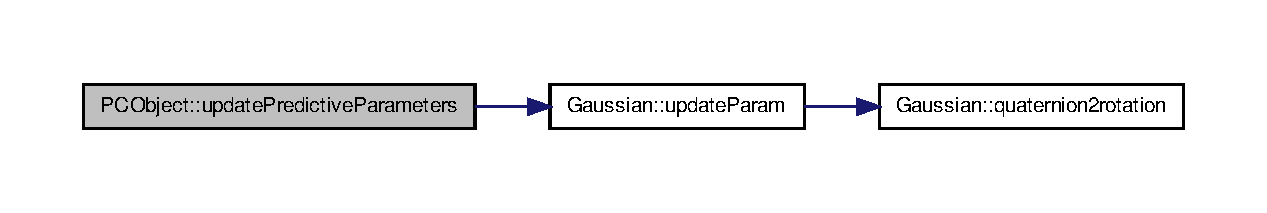
\includegraphics[width=350pt]{class_p_c_object_ae117d9276dd14490027029e8b87e150f_cgraph}
\end{center}
\end{figure}




\subsection{\-Member \-Data \-Documentation}
\hypertarget{class_p_c_object_ac94a79d35dece547fab98be2b70e9604}{\index{\-P\-C\-Object@{\-P\-C\-Object}!alpha@{alpha}}
\index{alpha@{alpha}!PCObject@{\-P\-C\-Object}}
\subsubsection[{alpha}]{\setlength{\rightskip}{0pt plus 5cm}double {\bf \-P\-C\-Object\-::alpha}}}\label{class_p_c_object_ac94a79d35dece547fab98be2b70e9604}
\hypertarget{class_p_c_object_a827d54b95fd8fbe64bd4f0fe7a7c1c80}{\index{\-P\-C\-Object@{\-P\-C\-Object}!centroid@{centroid}}
\index{centroid@{centroid}!PCObject@{\-P\-C\-Object}}
\subsubsection[{centroid}]{\setlength{\rightskip}{0pt plus 5cm}{\bf \-Point} {\bf \-P\-C\-Object\-::centroid}}}\label{class_p_c_object_a827d54b95fd8fbe64bd4f0fe7a7c1c80}
\hypertarget{class_p_c_object_a1e854b1f05424e21b57571c4d5d3a639}{\index{\-P\-C\-Object@{\-P\-C\-Object}!cnt@{cnt}}
\index{cnt@{cnt}!PCObject@{\-P\-C\-Object}}
\subsubsection[{cnt}]{\setlength{\rightskip}{0pt plus 5cm}int {\bf \-P\-C\-Object\-::cnt}}}\label{class_p_c_object_a1e854b1f05424e21b57571c4d5d3a639}
\hypertarget{class_p_c_object_ae08580ed200d25aa8304fde6f924c9f3}{\index{\-P\-C\-Object@{\-P\-C\-Object}!diff\-Weight@{diff\-Weight}}
\index{diff\-Weight@{diff\-Weight}!PCObject@{\-P\-C\-Object}}
\subsubsection[{diff\-Weight}]{\setlength{\rightskip}{0pt plus 5cm}double$\ast$ {\bf \-P\-C\-Object\-::diff\-Weight}}}\label{class_p_c_object_ae08580ed200d25aa8304fde6f924c9f3}
\hypertarget{class_p_c_object_aec75ff9931a685504afff6a7c1f78c02}{\index{\-P\-C\-Object@{\-P\-C\-Object}!dimension@{dimension}}
\index{dimension@{dimension}!PCObject@{\-P\-C\-Object}}
\subsubsection[{dimension}]{\setlength{\rightskip}{0pt plus 5cm}int {\bf \-P\-C\-Object\-::dimension}}}\label{class_p_c_object_aec75ff9931a685504afff6a7c1f78c02}
\hypertarget{class_p_c_object_a0d6dab1fe4edd99095e1fe236d4910a5}{\index{\-P\-C\-Object@{\-P\-C\-Object}!edges@{edges}}
\index{edges@{edges}!PCObject@{\-P\-C\-Object}}
\subsubsection[{edges}]{\setlength{\rightskip}{0pt plus 5cm}vector$<${\bf \-Edge}$>$ {\bf \-P\-C\-Object\-::edges}}}\label{class_p_c_object_a0d6dab1fe4edd99095e1fe236d4910a5}
\hypertarget{class_p_c_object_a959539770a6c61a3db3ef480140d1ed0}{\index{\-P\-C\-Object@{\-P\-C\-Object}!filtered\-Weight@{filtered\-Weight}}
\index{filtered\-Weight@{filtered\-Weight}!PCObject@{\-P\-C\-Object}}
\subsubsection[{filtered\-Weight}]{\setlength{\rightskip}{0pt plus 5cm}double {\bf \-P\-C\-Object\-::filtered\-Weight}}}\label{class_p_c_object_a959539770a6c61a3db3ef480140d1ed0}
\hypertarget{class_p_c_object_acbc764cefd102f6b184192ffa266510f}{\index{\-P\-C\-Object@{\-P\-C\-Object}!frame@{frame}}
\index{frame@{frame}!PCObject@{\-P\-C\-Object}}
\subsubsection[{frame}]{\setlength{\rightskip}{0pt plus 5cm}vector$<${\bf \-Gaussian}$\ast$$>$ {\bf \-P\-C\-Object\-::frame}}}\label{class_p_c_object_acbc764cefd102f6b184192ffa266510f}
\hypertarget{class_p_c_object_a2a0a0fe603bac2c80a43d4f6e224bf98}{\index{\-P\-C\-Object@{\-P\-C\-Object}!gaussian@{gaussian}}
\index{gaussian@{gaussian}!PCObject@{\-P\-C\-Object}}
\subsubsection[{gaussian}]{\setlength{\rightskip}{0pt plus 5cm}{\bf \-Gaussian} {\bf \-P\-C\-Object\-::gaussian}}}\label{class_p_c_object_a2a0a0fe603bac2c80a43d4f6e224bf98}
\hypertarget{class_p_c_object_a7d7a327eda5d75b554e2c83ba32a8517}{\index{\-P\-C\-Object@{\-P\-C\-Object}!gaussian\-Tracks@{gaussian\-Tracks}}
\index{gaussian\-Tracks@{gaussian\-Tracks}!PCObject@{\-P\-C\-Object}}
\subsubsection[{gaussian\-Tracks}]{\setlength{\rightskip}{0pt plus 5cm}{\bf \-Track\-Container}$<${\bf \-Gaussian}$>$$\ast$ {\bf \-P\-C\-Object\-::gaussian\-Tracks}}}\label{class_p_c_object_a7d7a327eda5d75b554e2c83ba32a8517}
\hypertarget{class_p_c_object_a7eae3d72d8dfedee042050dc80df4423}{\index{\-P\-C\-Object@{\-P\-C\-Object}!gmm@{gmm}}
\index{gmm@{gmm}!PCObject@{\-P\-C\-Object}}
\subsubsection[{gmm}]{\setlength{\rightskip}{0pt plus 5cm}vector$<${\bf \-Gaussian}$>$ {\bf \-P\-C\-Object\-::gmm}}}\label{class_p_c_object_a7eae3d72d8dfedee042050dc80df4423}
\hypertarget{class_p_c_object_a57cb1270dee62f9c65643f3cbe03347e}{\index{\-P\-C\-Object@{\-P\-C\-Object}!id@{id}}
\index{id@{id}!PCObject@{\-P\-C\-Object}}
\subsubsection[{id}]{\setlength{\rightskip}{0pt plus 5cm}int {\bf \-P\-C\-Object\-::id}}}\label{class_p_c_object_a57cb1270dee62f9c65643f3cbe03347e}
\hypertarget{class_p_c_object_aa921fc68268138b7f5026ec1ccaef619}{\index{\-P\-C\-Object@{\-P\-C\-Object}!imft\-Gaussians@{imft\-Gaussians}}
\index{imft\-Gaussians@{imft\-Gaussians}!PCObject@{\-P\-C\-Object}}
\subsubsection[{imft\-Gaussians}]{\setlength{\rightskip}{0pt plus 5cm}{\bf \-I\-M\-F\-T}$<${\bf \-Gaussian}$>$$\ast$ {\bf \-P\-C\-Object\-::imft\-Gaussians}}}\label{class_p_c_object_aa921fc68268138b7f5026ec1ccaef619}
\hypertarget{class_p_c_object_ab9a8f0b1f9d3b4851877e15e17582097}{\index{\-P\-C\-Object@{\-P\-C\-Object}!is\-Param\-Exist@{is\-Param\-Exist}}
\index{is\-Param\-Exist@{is\-Param\-Exist}!PCObject@{\-P\-C\-Object}}
\subsubsection[{is\-Param\-Exist}]{\setlength{\rightskip}{0pt plus 5cm}bool {\bf \-P\-C\-Object\-::is\-Param\-Exist}}}\label{class_p_c_object_ab9a8f0b1f9d3b4851877e15e17582097}
\hypertarget{class_p_c_object_a4ac23bed170d9a2993524e4b742c99a4}{\index{\-P\-C\-Object@{\-P\-C\-Object}!percent@{percent}}
\index{percent@{percent}!PCObject@{\-P\-C\-Object}}
\subsubsection[{percent}]{\setlength{\rightskip}{0pt plus 5cm}double {\bf \-P\-C\-Object\-::percent}}}\label{class_p_c_object_a4ac23bed170d9a2993524e4b742c99a4}
\hypertarget{class_p_c_object_a88519afe57e934c37b87cd74201573ae}{\index{\-P\-C\-Object@{\-P\-C\-Object}!points@{points}}
\index{points@{points}!PCObject@{\-P\-C\-Object}}
\subsubsection[{points}]{\setlength{\rightskip}{0pt plus 5cm}vector$<${\bf \-Point}$>$ {\bf \-P\-C\-Object\-::points}}}\label{class_p_c_object_a88519afe57e934c37b87cd74201573ae}
\hypertarget{class_p_c_object_a8737196626b96a2730810a9cee2330ed}{\index{\-P\-C\-Object@{\-P\-C\-Object}!scale@{scale}}
\index{scale@{scale}!PCObject@{\-P\-C\-Object}}
\subsubsection[{scale}]{\setlength{\rightskip}{0pt plus 5cm}double {\bf \-P\-C\-Object\-::scale}}}\label{class_p_c_object_a8737196626b96a2730810a9cee2330ed}
\hypertarget{class_p_c_object_ad5a0566f1118a4e70d1de788c7dd4c06}{\index{\-P\-C\-Object@{\-P\-C\-Object}!state@{state}}
\index{state@{state}!PCObject@{\-P\-C\-Object}}
\subsubsection[{state}]{\setlength{\rightskip}{0pt plus 5cm}{\bf \-S\-T\-A\-T\-E} {\bf \-P\-C\-Object\-::state}}}\label{class_p_c_object_ad5a0566f1118a4e70d1de788c7dd4c06}
\hypertarget{class_p_c_object_a2e2e26d46ec23849c062e9d28d349778}{\index{\-P\-C\-Object@{\-P\-C\-Object}!th\-\_\-edge@{th\-\_\-edge}}
\index{th\-\_\-edge@{th\-\_\-edge}!PCObject@{\-P\-C\-Object}}
\subsubsection[{th\-\_\-edge}]{\setlength{\rightskip}{0pt plus 5cm}double {\bf \-P\-C\-Object\-::th\-\_\-edge}}}\label{class_p_c_object_a2e2e26d46ec23849c062e9d28d349778}
\hypertarget{class_p_c_object_a5f09a7006b5499186fe9908143dfbee9}{\index{\-P\-C\-Object@{\-P\-C\-Object}!topology\-\_\-edge\-Map@{topology\-\_\-edge\-Map}}
\index{topology\-\_\-edge\-Map@{topology\-\_\-edge\-Map}!PCObject@{\-P\-C\-Object}}
\subsubsection[{topology\-\_\-edge\-Map}]{\setlength{\rightskip}{0pt plus 5cm}\-List\-Graph\-::\-Edge\-Map$<$double$>$$\ast$ {\bf \-P\-C\-Object\-::topology\-\_\-edge\-Map}}}\label{class_p_c_object_a5f09a7006b5499186fe9908143dfbee9}
\hypertarget{class_p_c_object_a1e2497e50fb2af6cf043d91b3d2e14c6}{\index{\-P\-C\-Object@{\-P\-C\-Object}!topology\-\_\-graph@{topology\-\_\-graph}}
\index{topology\-\_\-graph@{topology\-\_\-graph}!PCObject@{\-P\-C\-Object}}
\subsubsection[{topology\-\_\-graph}]{\setlength{\rightskip}{0pt plus 5cm}\-List\-Graph$\ast$ {\bf \-P\-C\-Object\-::topology\-\_\-graph}}}\label{class_p_c_object_a1e2497e50fb2af6cf043d91b3d2e14c6}
\hypertarget{class_p_c_object_a99eafcc86b98ec0f1d165b8a96d351dc}{\index{\-P\-C\-Object@{\-P\-C\-Object}!topology\-\_\-node\-Map@{topology\-\_\-node\-Map}}
\index{topology\-\_\-node\-Map@{topology\-\_\-node\-Map}!PCObject@{\-P\-C\-Object}}
\subsubsection[{topology\-\_\-node\-Map}]{\setlength{\rightskip}{0pt plus 5cm}\-List\-Graph\-::\-Node\-Map$<${\bf \-Gaussian}$>$$\ast$ {\bf \-P\-C\-Object\-::topology\-\_\-node\-Map}}}\label{class_p_c_object_a99eafcc86b98ec0f1d165b8a96d351dc}
\hypertarget{class_p_c_object_aca5e8c66727c01980551ac8744bfb26a}{\index{\-P\-C\-Object@{\-P\-C\-Object}!trans\-\_\-param@{trans\-\_\-param}}
\index{trans\-\_\-param@{trans\-\_\-param}!PCObject@{\-P\-C\-Object}}
\subsubsection[{trans\-\_\-param}]{\setlength{\rightskip}{0pt plus 5cm}vnl\-\_\-vector$<$double$>$ {\bf \-P\-C\-Object\-::trans\-\_\-param}}}\label{class_p_c_object_aca5e8c66727c01980551ac8744bfb26a}
\hypertarget{class_p_c_object_a1606ff67b8422eac1ee46849bffdb69a}{\index{\-P\-C\-Object@{\-P\-C\-Object}!window\-\_\-long@{window\-\_\-long}}
\index{window\-\_\-long@{window\-\_\-long}!PCObject@{\-P\-C\-Object}}
\subsubsection[{window\-\_\-long}]{\setlength{\rightskip}{0pt plus 5cm}int {\bf \-P\-C\-Object\-::window\-\_\-long}\hspace{0.3cm}{\ttfamily  \mbox{[}private\mbox{]}}}}\label{class_p_c_object_a1606ff67b8422eac1ee46849bffdb69a}
\hypertarget{class_p_c_object_a6c90b358d6d19ab437841f829e448b7c}{\index{\-P\-C\-Object@{\-P\-C\-Object}!window\-\_\-short@{window\-\_\-short}}
\index{window\-\_\-short@{window\-\_\-short}!PCObject@{\-P\-C\-Object}}
\subsubsection[{window\-\_\-short}]{\setlength{\rightskip}{0pt plus 5cm}int {\bf \-P\-C\-Object\-::window\-\_\-short}\hspace{0.3cm}{\ttfamily  \mbox{[}private\mbox{]}}}}\label{class_p_c_object_a6c90b358d6d19ab437841f829e448b7c}


\-The documentation for this class was generated from the following files\-:\begin{DoxyCompactItemize}
\item 
/home/koosy/koosywork/pmot\-\_\-realtime/pmot\-\_\-realtime/src/\hyperlink{pcobject_8h}{pcobject.\-h}\item 
/home/koosy/koosywork/pmot\-\_\-realtime/pmot\-\_\-realtime/src/\hyperlink{pcobject_8cpp}{pcobject.\-cpp}\end{DoxyCompactItemize}

\hypertarget{class_p_c_object_container}{\section{\-P\-C\-Object\-Container \-Class \-Reference}
\label{class_p_c_object_container}\index{\-P\-C\-Object\-Container@{\-P\-C\-Object\-Container}}
}


{\ttfamily \#include $<$pcobjectcontainer.\-h$>$}

\subsection*{\-Public \-Member \-Functions}
\begin{DoxyCompactItemize}
\item 
\hyperlink{class_p_c_object_container_af21d443878f8f8c78e32db3ba7bdcd0e}{\-P\-C\-Object\-Container} ()
\item 
\hyperlink{class_p_c_object_container_a9ba8e8bca146e65e310f3acba0405617}{\-P\-C\-Object\-Container} (\hyperlink{common_8h_a36884aa4a3c181fa4c284d79329ad166}{\-Cloud\-Ptr} \-\_\-p\-Cloud)
\item 
\hyperlink{class_p_c_object_container_a62369d4a9a192b8e7266b82065362b01}{$\sim$\-P\-C\-Object\-Container} ()
\item 
int \hyperlink{class_p_c_object_container_a3028b503e5f50ee7ba14b9224cdc411d}{num\-Objects} ()
\item 
bool \hyperlink{class_p_c_object_container_a22f12c64c44f6d5881762aedad0cfb02}{delete\-Object} (int id)
\item 
void \hyperlink{class_p_c_object_container_a2d8ab397f1a69ceec7a916905565f19f}{make\-New\-Object} (\hyperlink{class_p_c_object}{\-P\-C\-Object} \&object)
\item 
void \hyperlink{class_p_c_object_container_af032c7cb3ebb37bdb515f9192f609b0e}{init\-G\-M\-M} (double \hyperlink{class_p_c_object_container_af11c2139d36c285b66b3b56ac5b3f96e}{scale}, double percent)
\item 
void \hyperlink{class_p_c_object_container_a0ef13acb954dbf3d99a743c6a1983576}{clear\-All} ()
\end{DoxyCompactItemize}
\subsection*{\-Public \-Attributes}
\begin{DoxyCompactItemize}
\item 
vector$<$ \hyperlink{class_p_c_object}{\-P\-C\-Object} $>$ \hyperlink{class_p_c_object_container_a92c4994a8b244c531bc1fb3391a9631e}{objects}
\item 
int \hyperlink{class_p_c_object_container_a59788043c1ab55a990cb05b26bf3633d}{num}
\end{DoxyCompactItemize}
\subsection*{\-Private \-Member \-Functions}
\begin{DoxyCompactItemize}
\item 
void \hyperlink{class_p_c_object_container_a257bc60b28b77508f0acbffc51e32074}{making\-Objects} ()
\end{DoxyCompactItemize}
\subsection*{\-Private \-Attributes}
\begin{DoxyCompactItemize}
\item 
\hyperlink{common_8h_a36884aa4a3c181fa4c284d79329ad166}{\-Cloud\-Ptr} \hyperlink{class_p_c_object_container_a9a06969ee10b3dcefccd13e76b7fa0db}{p\-Cloud}
\item 
double \hyperlink{class_p_c_object_container_af11c2139d36c285b66b3b56ac5b3f96e}{scale}
\end{DoxyCompactItemize}


\subsection{\-Constructor \& \-Destructor \-Documentation}
\hypertarget{class_p_c_object_container_af21d443878f8f8c78e32db3ba7bdcd0e}{\index{\-P\-C\-Object\-Container@{\-P\-C\-Object\-Container}!\-P\-C\-Object\-Container@{\-P\-C\-Object\-Container}}
\index{\-P\-C\-Object\-Container@{\-P\-C\-Object\-Container}!PCObjectContainer@{\-P\-C\-Object\-Container}}
\subsubsection[{\-P\-C\-Object\-Container}]{\setlength{\rightskip}{0pt plus 5cm}{\bf \-P\-C\-Object\-Container\-::\-P\-C\-Object\-Container} (
\begin{DoxyParamCaption}
{}
\end{DoxyParamCaption}
)}}\label{class_p_c_object_container_af21d443878f8f8c78e32db3ba7bdcd0e}
\hypertarget{class_p_c_object_container_a9ba8e8bca146e65e310f3acba0405617}{\index{\-P\-C\-Object\-Container@{\-P\-C\-Object\-Container}!\-P\-C\-Object\-Container@{\-P\-C\-Object\-Container}}
\index{\-P\-C\-Object\-Container@{\-P\-C\-Object\-Container}!PCObjectContainer@{\-P\-C\-Object\-Container}}
\subsubsection[{\-P\-C\-Object\-Container}]{\setlength{\rightskip}{0pt plus 5cm}{\bf \-P\-C\-Object\-Container\-::\-P\-C\-Object\-Container} (
\begin{DoxyParamCaption}
\item[{{\bf \-Cloud\-Ptr}}]{\-\_\-p\-Cloud}
\end{DoxyParamCaption}
)}}\label{class_p_c_object_container_a9ba8e8bca146e65e310f3acba0405617}


\-Here is the call graph for this function\-:
\nopagebreak
\begin{figure}[H]
\begin{center}
\leavevmode
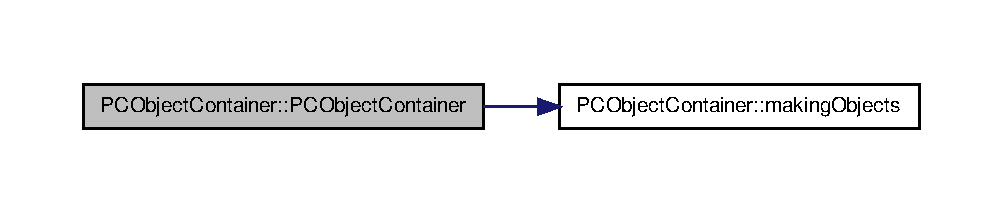
\includegraphics[width=350pt]{class_p_c_object_container_a9ba8e8bca146e65e310f3acba0405617_cgraph}
\end{center}
\end{figure}


\hypertarget{class_p_c_object_container_a62369d4a9a192b8e7266b82065362b01}{\index{\-P\-C\-Object\-Container@{\-P\-C\-Object\-Container}!$\sim$\-P\-C\-Object\-Container@{$\sim$\-P\-C\-Object\-Container}}
\index{$\sim$\-P\-C\-Object\-Container@{$\sim$\-P\-C\-Object\-Container}!PCObjectContainer@{\-P\-C\-Object\-Container}}
\subsubsection[{$\sim$\-P\-C\-Object\-Container}]{\setlength{\rightskip}{0pt plus 5cm}{\bf \-P\-C\-Object\-Container\-::$\sim$\-P\-C\-Object\-Container} (
\begin{DoxyParamCaption}
{}
\end{DoxyParamCaption}
)}}\label{class_p_c_object_container_a62369d4a9a192b8e7266b82065362b01}


\subsection{\-Member \-Function \-Documentation}
\hypertarget{class_p_c_object_container_a0ef13acb954dbf3d99a743c6a1983576}{\index{\-P\-C\-Object\-Container@{\-P\-C\-Object\-Container}!clear\-All@{clear\-All}}
\index{clear\-All@{clear\-All}!PCObjectContainer@{\-P\-C\-Object\-Container}}
\subsubsection[{clear\-All}]{\setlength{\rightskip}{0pt plus 5cm}void {\bf \-P\-C\-Object\-Container\-::clear\-All} (
\begin{DoxyParamCaption}
{}
\end{DoxyParamCaption}
)}}\label{class_p_c_object_container_a0ef13acb954dbf3d99a743c6a1983576}


\-Here is the caller graph for this function\-:
\nopagebreak
\begin{figure}[H]
\begin{center}
\leavevmode
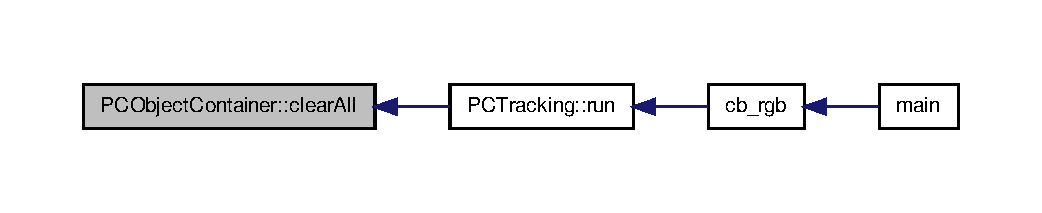
\includegraphics[width=350pt]{class_p_c_object_container_a0ef13acb954dbf3d99a743c6a1983576_icgraph}
\end{center}
\end{figure}


\hypertarget{class_p_c_object_container_a22f12c64c44f6d5881762aedad0cfb02}{\index{\-P\-C\-Object\-Container@{\-P\-C\-Object\-Container}!delete\-Object@{delete\-Object}}
\index{delete\-Object@{delete\-Object}!PCObjectContainer@{\-P\-C\-Object\-Container}}
\subsubsection[{delete\-Object}]{\setlength{\rightskip}{0pt plus 5cm}bool {\bf \-P\-C\-Object\-Container\-::delete\-Object} (
\begin{DoxyParamCaption}
\item[{int}]{id}
\end{DoxyParamCaption}
)}}\label{class_p_c_object_container_a22f12c64c44f6d5881762aedad0cfb02}
\hypertarget{class_p_c_object_container_af032c7cb3ebb37bdb515f9192f609b0e}{\index{\-P\-C\-Object\-Container@{\-P\-C\-Object\-Container}!init\-G\-M\-M@{init\-G\-M\-M}}
\index{init\-G\-M\-M@{init\-G\-M\-M}!PCObjectContainer@{\-P\-C\-Object\-Container}}
\subsubsection[{init\-G\-M\-M}]{\setlength{\rightskip}{0pt plus 5cm}void {\bf \-P\-C\-Object\-Container\-::init\-G\-M\-M} (
\begin{DoxyParamCaption}
\item[{double}]{scale, }
\item[{double}]{percent}
\end{DoxyParamCaption}
)}}\label{class_p_c_object_container_af032c7cb3ebb37bdb515f9192f609b0e}


\-Here is the call graph for this function\-:
\nopagebreak
\begin{figure}[H]
\begin{center}
\leavevmode
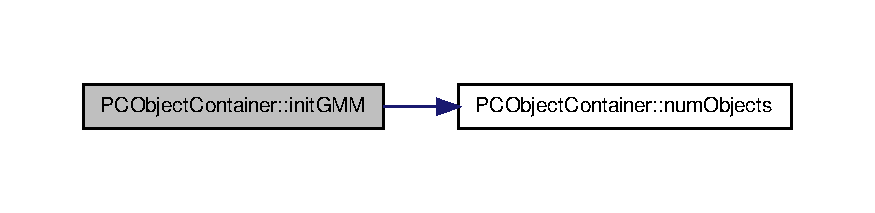
\includegraphics[width=350pt]{class_p_c_object_container_af032c7cb3ebb37bdb515f9192f609b0e_cgraph}
\end{center}
\end{figure}


\hypertarget{class_p_c_object_container_a2d8ab397f1a69ceec7a916905565f19f}{\index{\-P\-C\-Object\-Container@{\-P\-C\-Object\-Container}!make\-New\-Object@{make\-New\-Object}}
\index{make\-New\-Object@{make\-New\-Object}!PCObjectContainer@{\-P\-C\-Object\-Container}}
\subsubsection[{make\-New\-Object}]{\setlength{\rightskip}{0pt plus 5cm}void {\bf \-P\-C\-Object\-Container\-::make\-New\-Object} (
\begin{DoxyParamCaption}
\item[{{\bf \-P\-C\-Object} \&}]{object}
\end{DoxyParamCaption}
)}}\label{class_p_c_object_container_a2d8ab397f1a69ceec7a916905565f19f}


\-Here is the caller graph for this function\-:
\nopagebreak
\begin{figure}[H]
\begin{center}
\leavevmode
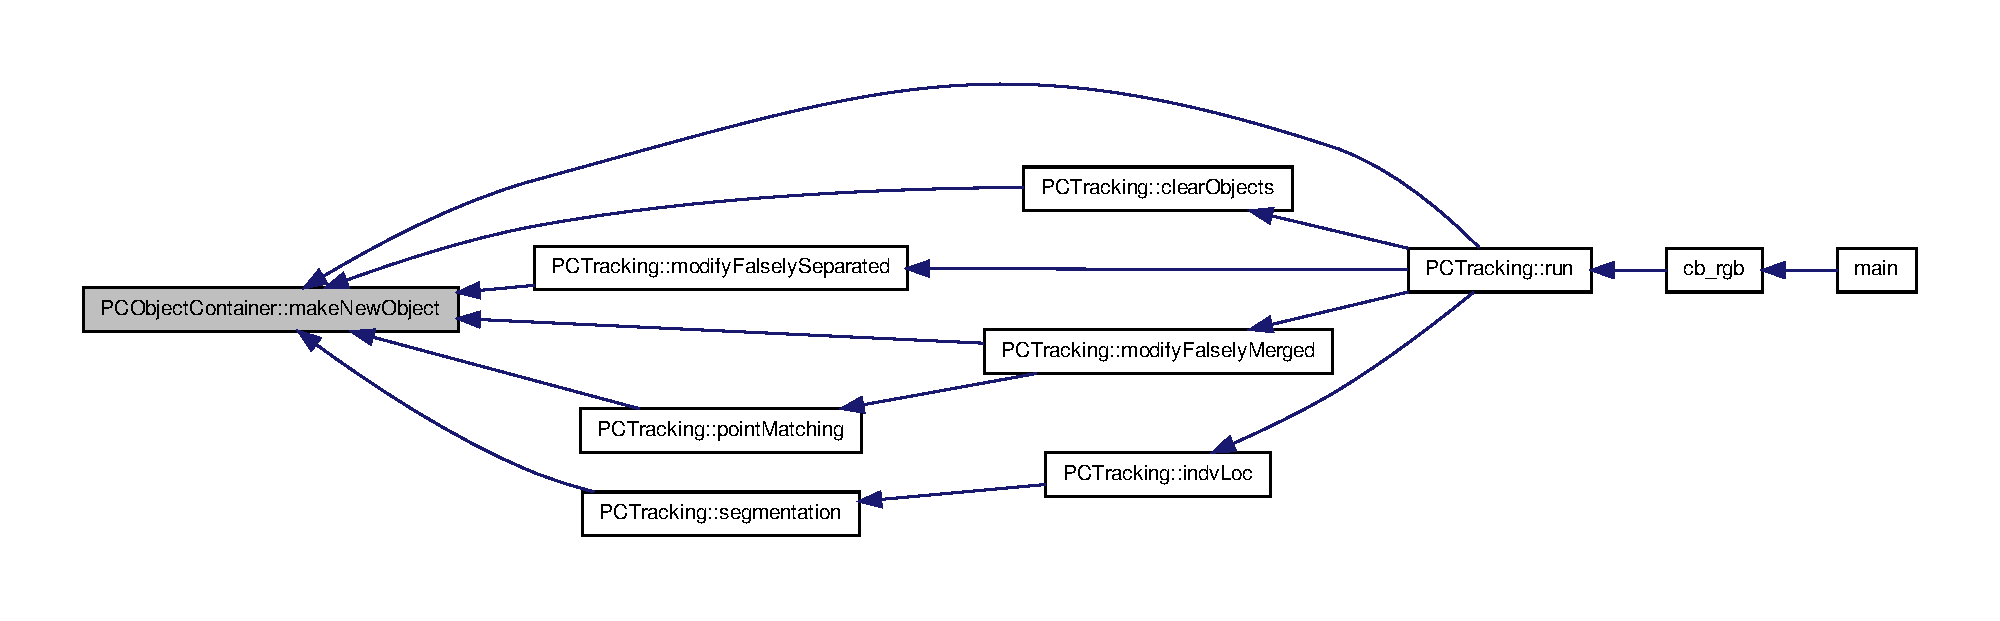
\includegraphics[width=350pt]{class_p_c_object_container_a2d8ab397f1a69ceec7a916905565f19f_icgraph}
\end{center}
\end{figure}


\hypertarget{class_p_c_object_container_a257bc60b28b77508f0acbffc51e32074}{\index{\-P\-C\-Object\-Container@{\-P\-C\-Object\-Container}!making\-Objects@{making\-Objects}}
\index{making\-Objects@{making\-Objects}!PCObjectContainer@{\-P\-C\-Object\-Container}}
\subsubsection[{making\-Objects}]{\setlength{\rightskip}{0pt plus 5cm}void {\bf \-P\-C\-Object\-Container\-::making\-Objects} (
\begin{DoxyParamCaption}
{}
\end{DoxyParamCaption}
)\hspace{0.3cm}{\ttfamily  \mbox{[}private\mbox{]}}}}\label{class_p_c_object_container_a257bc60b28b77508f0acbffc51e32074}


\-Here is the caller graph for this function\-:
\nopagebreak
\begin{figure}[H]
\begin{center}
\leavevmode
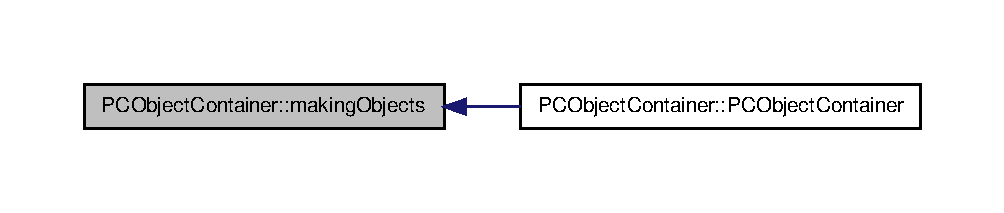
\includegraphics[width=350pt]{class_p_c_object_container_a257bc60b28b77508f0acbffc51e32074_icgraph}
\end{center}
\end{figure}


\hypertarget{class_p_c_object_container_a3028b503e5f50ee7ba14b9224cdc411d}{\index{\-P\-C\-Object\-Container@{\-P\-C\-Object\-Container}!num\-Objects@{num\-Objects}}
\index{num\-Objects@{num\-Objects}!PCObjectContainer@{\-P\-C\-Object\-Container}}
\subsubsection[{num\-Objects}]{\setlength{\rightskip}{0pt plus 5cm}int {\bf \-P\-C\-Object\-Container\-::num\-Objects} (
\begin{DoxyParamCaption}
{}
\end{DoxyParamCaption}
)\hspace{0.3cm}{\ttfamily  \mbox{[}inline\mbox{]}}}}\label{class_p_c_object_container_a3028b503e5f50ee7ba14b9224cdc411d}


\-Here is the caller graph for this function\-:
\nopagebreak
\begin{figure}[H]
\begin{center}
\leavevmode
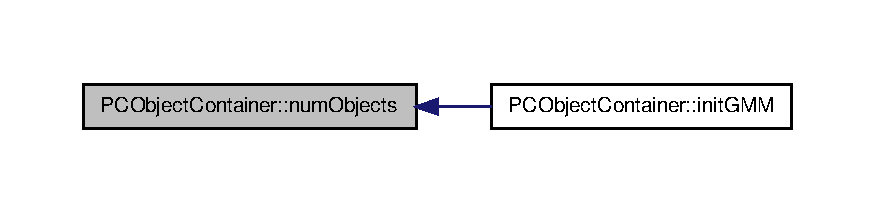
\includegraphics[width=350pt]{class_p_c_object_container_a3028b503e5f50ee7ba14b9224cdc411d_icgraph}
\end{center}
\end{figure}




\subsection{\-Member \-Data \-Documentation}
\hypertarget{class_p_c_object_container_a59788043c1ab55a990cb05b26bf3633d}{\index{\-P\-C\-Object\-Container@{\-P\-C\-Object\-Container}!num@{num}}
\index{num@{num}!PCObjectContainer@{\-P\-C\-Object\-Container}}
\subsubsection[{num}]{\setlength{\rightskip}{0pt plus 5cm}int {\bf \-P\-C\-Object\-Container\-::num}}}\label{class_p_c_object_container_a59788043c1ab55a990cb05b26bf3633d}
\hypertarget{class_p_c_object_container_a92c4994a8b244c531bc1fb3391a9631e}{\index{\-P\-C\-Object\-Container@{\-P\-C\-Object\-Container}!objects@{objects}}
\index{objects@{objects}!PCObjectContainer@{\-P\-C\-Object\-Container}}
\subsubsection[{objects}]{\setlength{\rightskip}{0pt plus 5cm}vector$<${\bf \-P\-C\-Object}$>$ {\bf \-P\-C\-Object\-Container\-::objects}}}\label{class_p_c_object_container_a92c4994a8b244c531bc1fb3391a9631e}
\hypertarget{class_p_c_object_container_a9a06969ee10b3dcefccd13e76b7fa0db}{\index{\-P\-C\-Object\-Container@{\-P\-C\-Object\-Container}!p\-Cloud@{p\-Cloud}}
\index{p\-Cloud@{p\-Cloud}!PCObjectContainer@{\-P\-C\-Object\-Container}}
\subsubsection[{p\-Cloud}]{\setlength{\rightskip}{0pt plus 5cm}{\bf \-Cloud\-Ptr} {\bf \-P\-C\-Object\-Container\-::p\-Cloud}\hspace{0.3cm}{\ttfamily  \mbox{[}private\mbox{]}}}}\label{class_p_c_object_container_a9a06969ee10b3dcefccd13e76b7fa0db}
\hypertarget{class_p_c_object_container_af11c2139d36c285b66b3b56ac5b3f96e}{\index{\-P\-C\-Object\-Container@{\-P\-C\-Object\-Container}!scale@{scale}}
\index{scale@{scale}!PCObjectContainer@{\-P\-C\-Object\-Container}}
\subsubsection[{scale}]{\setlength{\rightskip}{0pt plus 5cm}double {\bf \-P\-C\-Object\-Container\-::scale}\hspace{0.3cm}{\ttfamily  \mbox{[}private\mbox{]}}}}\label{class_p_c_object_container_af11c2139d36c285b66b3b56ac5b3f96e}


\-The documentation for this class was generated from the following files\-:\begin{DoxyCompactItemize}
\item 
/home/koosy/koosywork/pmot\-\_\-realtime/pmot\-\_\-realtime/src/\hyperlink{pcobjectcontainer_8h}{pcobjectcontainer.\-h}\item 
/home/koosy/koosywork/pmot\-\_\-realtime/pmot\-\_\-realtime/src/\hyperlink{pcobjectcontainer_8cpp}{pcobjectcontainer.\-cpp}\end{DoxyCompactItemize}

\hypertarget{class_p_c_track_container}{\section{\-P\-C\-Track\-Container \-Class \-Reference}
\label{class_p_c_track_container}\index{\-P\-C\-Track\-Container@{\-P\-C\-Track\-Container}}
}


{\ttfamily \#include $<$pctrackcontainer.\-h$>$}



\-Inheritance diagram for \-P\-C\-Track\-Container\-:
\nopagebreak
\begin{figure}[H]
\begin{center}
\leavevmode
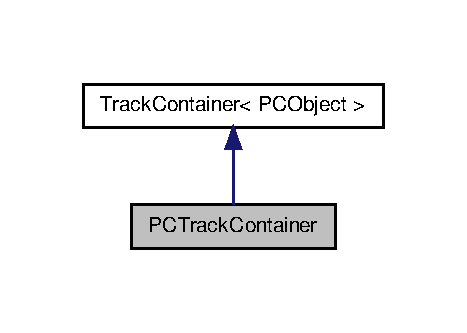
\includegraphics[width=224pt]{class_p_c_track_container__inherit__graph}
\end{center}
\end{figure}


\-Collaboration diagram for \-P\-C\-Track\-Container\-:
\nopagebreak
\begin{figure}[H]
\begin{center}
\leavevmode
\includegraphics[width=224pt]{class_p_c_track_container__coll__graph}
\end{center}
\end{figure}
\subsection*{\-Public \-Member \-Functions}
\begin{DoxyCompactItemize}
\item 
\hyperlink{class_p_c_track_container_a57b7ba43e31583d6e0c2660ce79c6e0a}{\-P\-C\-Track\-Container} ()
\item 
\hyperlink{class_p_c_track_container_aa3f42b51f7c0148dd8cf2936194ab9dc}{\-P\-C\-Track\-Container} (int \-\_\-max\-Frame=1000)
\item 
void \hyperlink{class_p_c_track_container_a4881bd9b8b1692193f07e48c3389c5db}{to\-Point\-Cloud\-X\-Y\-Z\-I} (\hyperlink{class_p_c_track_container_ad70a8e8d9236664790fd8d76a2ebeadb}{\-Cloud} \&cloud\-Out)
\item 
visualization\-\_\-msgs\-::\-Marker\-Array \hyperlink{class_p_c_track_container_acda2db186798fe99100c11c622d93f27}{to\-Marker\-Gaussians} ()
\item 
visualization\-\_\-msgs\-::\-Marker\-Array \hyperlink{class_p_c_track_container_a6b4e74ccf8ffbc81eef4843b5b300fa3}{to\-Marker\-G\-M\-Ms} ()
\item 
visualization\-\_\-msgs\-::\-Marker\-Array \hyperlink{class_p_c_track_container_ab62240a09d2587f15cf0f346bdac9b14}{old\-Gaussians} ()
\item 
visualization\-\_\-msgs\-::\-Marker\-Array \hyperlink{class_p_c_track_container_a5bd37d304d5fab465535c395d3c8a86f}{to\-Marker\-I\-Ds} ()
\item 
visualization\-\_\-msgs\-::\-Marker\-Array \hyperlink{class_p_c_track_container_a584a5f8b8043959c78f415f7b98d70bf}{old\-Marker\-I\-Ds} ()
\item 
visualization\-\_\-msgs\-::\-Marker \hyperlink{class_p_c_track_container_a4330fcbefe00381504c8493b0c8c4c4b}{to\-Marker\-Edges} ()
\item 
void \hyperlink{class_p_c_track_container_a661c9e504ba3f4a2e9b4bf5d12d5a76c}{evaluate} ()
\item 
void \hyperlink{class_p_c_track_container_a32a1137979b67b2bba51a768a6d2398b}{iros2014} ()
\end{DoxyCompactItemize}
\subsection*{\-Public \-Attributes}
\begin{DoxyCompactItemize}
\item 
int \hyperlink{class_p_c_track_container_a5ac828bfcaa2932955a67c3e478849c0}{num\-True\-Points}
\item 
int \hyperlink{class_p_c_track_container_a8e9b9d663f2227fad5f9a6743d8dd254}{num\-False\-Points}
\item 
int \hyperlink{class_p_c_track_container_a8289947fa7796de78ec1d84e7768db83}{num\-Total\-Points}
\item 
bool \hyperlink{class_p_c_track_container_a51514b479f4c23c13f412dc36766f73f}{is\-Updated}
\end{DoxyCompactItemize}
\subsection*{\-Private \-Types}
\begin{DoxyCompactItemize}
\item 
typedef pcl\-::\-Point\-X\-Y\-Z\-R\-G\-B \hyperlink{class_p_c_track_container_a37571d1fb0e896825033974c21a59ada}{\-Point\-T}
\item 
typedef pcl\-::\-Point\-Cloud$<$ \hyperlink{class_p_c_track_container_a37571d1fb0e896825033974c21a59ada}{\-Point\-T} $>$ \hyperlink{class_p_c_track_container_ad70a8e8d9236664790fd8d76a2ebeadb}{\-Cloud}
\item 
typedef \-Cloud\-::\-Ptr \hyperlink{class_p_c_track_container_a6e14769099ac04f16c881162f9397f56}{\-Cloud\-Ptr}
\item 
typedef \-Cloud\-::\-Const\-Ptr \hyperlink{class_p_c_track_container_a14e4333a2498a4a5728e888fc473b129}{\-Cloud\-Const\-Ptr}
\end{DoxyCompactItemize}
\subsection*{\-Private \-Member \-Functions}
\begin{DoxyCompactItemize}
\item 
float \hyperlink{class_p_c_track_container_a048f09bbd1d6c1655e1d58a113e86b1d}{\-S\-I\-G\-N} (float x)
\item 
float \hyperlink{class_p_c_track_container_ab722f94e8a660331d1c987a91af50179}{\-N\-O\-R\-M} (float a, float \hyperlink{class_track_container_a090d3d6e83acad80cad082cd718a4ab3}{b}, float c, float d)
\item 
void \hyperlink{class_p_c_track_container_a5d2ad9da112f92800e67d2da8f1ac531}{eigen\-Ordering} (const \-Eigen\-::\-Vector3d \&values, const \-Eigen\-::\-Matrix3d \&vectors, \-Eigen\-::\-Vector3d \&values\-\_\-ordered, \-Eigen\-::\-Matrix3d \&vectors\-\_\-ordered)
\end{DoxyCompactItemize}
\subsection*{\-Private \-Attributes}
\begin{DoxyCompactItemize}
\item 
int \hyperlink{class_p_c_track_container_afa0c55015d7b49548fa196d3091dacba}{max\-Frame}
\item 
vector$<$ int $>$ \hyperlink{class_p_c_track_container_a3bc617cd354340024249e246b9843a67}{old\-Gaussians\-Id}
\item 
vector$<$ int $>$ \hyperlink{class_p_c_track_container_ad2a1026f52411833d07d1fbf741e7cd5}{old\-Track\-I\-Ds}
\end{DoxyCompactItemize}


\subsection{\-Member \-Typedef \-Documentation}
\hypertarget{class_p_c_track_container_ad70a8e8d9236664790fd8d76a2ebeadb}{\index{\-P\-C\-Track\-Container@{\-P\-C\-Track\-Container}!\-Cloud@{\-Cloud}}
\index{\-Cloud@{\-Cloud}!PCTrackContainer@{\-P\-C\-Track\-Container}}
\subsubsection[{\-Cloud}]{\setlength{\rightskip}{0pt plus 5cm}typedef pcl\-::\-Point\-Cloud$<${\bf \-Point\-T}$>$ {\bf \-P\-C\-Track\-Container\-::\-Cloud}\hspace{0.3cm}{\ttfamily  \mbox{[}private\mbox{]}}}}\label{class_p_c_track_container_ad70a8e8d9236664790fd8d76a2ebeadb}
\hypertarget{class_p_c_track_container_a14e4333a2498a4a5728e888fc473b129}{\index{\-P\-C\-Track\-Container@{\-P\-C\-Track\-Container}!\-Cloud\-Const\-Ptr@{\-Cloud\-Const\-Ptr}}
\index{\-Cloud\-Const\-Ptr@{\-Cloud\-Const\-Ptr}!PCTrackContainer@{\-P\-C\-Track\-Container}}
\subsubsection[{\-Cloud\-Const\-Ptr}]{\setlength{\rightskip}{0pt plus 5cm}typedef \-Cloud\-::\-Const\-Ptr {\bf \-P\-C\-Track\-Container\-::\-Cloud\-Const\-Ptr}\hspace{0.3cm}{\ttfamily  \mbox{[}private\mbox{]}}}}\label{class_p_c_track_container_a14e4333a2498a4a5728e888fc473b129}
\hypertarget{class_p_c_track_container_a6e14769099ac04f16c881162f9397f56}{\index{\-P\-C\-Track\-Container@{\-P\-C\-Track\-Container}!\-Cloud\-Ptr@{\-Cloud\-Ptr}}
\index{\-Cloud\-Ptr@{\-Cloud\-Ptr}!PCTrackContainer@{\-P\-C\-Track\-Container}}
\subsubsection[{\-Cloud\-Ptr}]{\setlength{\rightskip}{0pt plus 5cm}typedef \-Cloud\-::\-Ptr {\bf \-P\-C\-Track\-Container\-::\-Cloud\-Ptr}\hspace{0.3cm}{\ttfamily  \mbox{[}private\mbox{]}}}}\label{class_p_c_track_container_a6e14769099ac04f16c881162f9397f56}
\hypertarget{class_p_c_track_container_a37571d1fb0e896825033974c21a59ada}{\index{\-P\-C\-Track\-Container@{\-P\-C\-Track\-Container}!\-Point\-T@{\-Point\-T}}
\index{\-Point\-T@{\-Point\-T}!PCTrackContainer@{\-P\-C\-Track\-Container}}
\subsubsection[{\-Point\-T}]{\setlength{\rightskip}{0pt plus 5cm}typedef pcl\-::\-Point\-X\-Y\-Z\-R\-G\-B {\bf \-P\-C\-Track\-Container\-::\-Point\-T}\hspace{0.3cm}{\ttfamily  \mbox{[}private\mbox{]}}}}\label{class_p_c_track_container_a37571d1fb0e896825033974c21a59ada}


\subsection{\-Constructor \& \-Destructor \-Documentation}
\hypertarget{class_p_c_track_container_a57b7ba43e31583d6e0c2660ce79c6e0a}{\index{\-P\-C\-Track\-Container@{\-P\-C\-Track\-Container}!\-P\-C\-Track\-Container@{\-P\-C\-Track\-Container}}
\index{\-P\-C\-Track\-Container@{\-P\-C\-Track\-Container}!PCTrackContainer@{\-P\-C\-Track\-Container}}
\subsubsection[{\-P\-C\-Track\-Container}]{\setlength{\rightskip}{0pt plus 5cm}{\bf \-P\-C\-Track\-Container\-::\-P\-C\-Track\-Container} (
\begin{DoxyParamCaption}
{}
\end{DoxyParamCaption}
)}}\label{class_p_c_track_container_a57b7ba43e31583d6e0c2660ce79c6e0a}
\hypertarget{class_p_c_track_container_aa3f42b51f7c0148dd8cf2936194ab9dc}{\index{\-P\-C\-Track\-Container@{\-P\-C\-Track\-Container}!\-P\-C\-Track\-Container@{\-P\-C\-Track\-Container}}
\index{\-P\-C\-Track\-Container@{\-P\-C\-Track\-Container}!PCTrackContainer@{\-P\-C\-Track\-Container}}
\subsubsection[{\-P\-C\-Track\-Container}]{\setlength{\rightskip}{0pt plus 5cm}{\bf \-P\-C\-Track\-Container\-::\-P\-C\-Track\-Container} (
\begin{DoxyParamCaption}
\item[{int}]{\-\_\-max\-Frame = {\ttfamily 1000}}
\end{DoxyParamCaption}
)}}\label{class_p_c_track_container_aa3f42b51f7c0148dd8cf2936194ab9dc}


\subsection{\-Member \-Function \-Documentation}
\hypertarget{class_p_c_track_container_a5d2ad9da112f92800e67d2da8f1ac531}{\index{\-P\-C\-Track\-Container@{\-P\-C\-Track\-Container}!eigen\-Ordering@{eigen\-Ordering}}
\index{eigen\-Ordering@{eigen\-Ordering}!PCTrackContainer@{\-P\-C\-Track\-Container}}
\subsubsection[{eigen\-Ordering}]{\setlength{\rightskip}{0pt plus 5cm}void {\bf \-P\-C\-Track\-Container\-::eigen\-Ordering} (
\begin{DoxyParamCaption}
\item[{const \-Eigen\-::\-Vector3d \&}]{values, }
\item[{const \-Eigen\-::\-Matrix3d \&}]{vectors, }
\item[{\-Eigen\-::\-Vector3d \&}]{values\-\_\-ordered, }
\item[{\-Eigen\-::\-Matrix3d \&}]{vectors\-\_\-ordered}
\end{DoxyParamCaption}
)\hspace{0.3cm}{\ttfamily  \mbox{[}private\mbox{]}}}}\label{class_p_c_track_container_a5d2ad9da112f92800e67d2da8f1ac531}


\-Here is the caller graph for this function\-:
\nopagebreak
\begin{figure}[H]
\begin{center}
\leavevmode
\includegraphics[width=350pt]{class_p_c_track_container_a5d2ad9da112f92800e67d2da8f1ac531_icgraph}
\end{center}
\end{figure}


\hypertarget{class_p_c_track_container_a661c9e504ba3f4a2e9b4bf5d12d5a76c}{\index{\-P\-C\-Track\-Container@{\-P\-C\-Track\-Container}!evaluate@{evaluate}}
\index{evaluate@{evaluate}!PCTrackContainer@{\-P\-C\-Track\-Container}}
\subsubsection[{evaluate}]{\setlength{\rightskip}{0pt plus 5cm}void {\bf \-P\-C\-Track\-Container\-::evaluate} (
\begin{DoxyParamCaption}
{}
\end{DoxyParamCaption}
)}}\label{class_p_c_track_container_a661c9e504ba3f4a2e9b4bf5d12d5a76c}


\-Here is the call graph for this function\-:
\nopagebreak
\begin{figure}[H]
\begin{center}
\leavevmode
\includegraphics[width=350pt]{class_p_c_track_container_a661c9e504ba3f4a2e9b4bf5d12d5a76c_cgraph}
\end{center}
\end{figure}


\hypertarget{class_p_c_track_container_a32a1137979b67b2bba51a768a6d2398b}{\index{\-P\-C\-Track\-Container@{\-P\-C\-Track\-Container}!iros2014@{iros2014}}
\index{iros2014@{iros2014}!PCTrackContainer@{\-P\-C\-Track\-Container}}
\subsubsection[{iros2014}]{\setlength{\rightskip}{0pt plus 5cm}void {\bf \-P\-C\-Track\-Container\-::iros2014} (
\begin{DoxyParamCaption}
{}
\end{DoxyParamCaption}
)}}\label{class_p_c_track_container_a32a1137979b67b2bba51a768a6d2398b}


\-Here is the call graph for this function\-:
\nopagebreak
\begin{figure}[H]
\begin{center}
\leavevmode
\includegraphics[width=350pt]{class_p_c_track_container_a32a1137979b67b2bba51a768a6d2398b_cgraph}
\end{center}
\end{figure}


\hypertarget{class_p_c_track_container_ab722f94e8a660331d1c987a91af50179}{\index{\-P\-C\-Track\-Container@{\-P\-C\-Track\-Container}!\-N\-O\-R\-M@{\-N\-O\-R\-M}}
\index{\-N\-O\-R\-M@{\-N\-O\-R\-M}!PCTrackContainer@{\-P\-C\-Track\-Container}}
\subsubsection[{\-N\-O\-R\-M}]{\setlength{\rightskip}{0pt plus 5cm}float {\bf \-P\-C\-Track\-Container\-::\-N\-O\-R\-M} (
\begin{DoxyParamCaption}
\item[{float}]{a, }
\item[{float}]{b, }
\item[{float}]{c, }
\item[{float}]{d}
\end{DoxyParamCaption}
)\hspace{0.3cm}{\ttfamily  \mbox{[}inline, private\mbox{]}}}}\label{class_p_c_track_container_ab722f94e8a660331d1c987a91af50179}
\hypertarget{class_p_c_track_container_ab62240a09d2587f15cf0f346bdac9b14}{\index{\-P\-C\-Track\-Container@{\-P\-C\-Track\-Container}!old\-Gaussians@{old\-Gaussians}}
\index{old\-Gaussians@{old\-Gaussians}!PCTrackContainer@{\-P\-C\-Track\-Container}}
\subsubsection[{old\-Gaussians}]{\setlength{\rightskip}{0pt plus 5cm}visualization\-\_\-msgs\-::\-Marker\-Array {\bf \-P\-C\-Track\-Container\-::old\-Gaussians} (
\begin{DoxyParamCaption}
{}
\end{DoxyParamCaption}
)}}\label{class_p_c_track_container_ab62240a09d2587f15cf0f346bdac9b14}


\-Here is the caller graph for this function\-:
\nopagebreak
\begin{figure}[H]
\begin{center}
\leavevmode
\includegraphics[width=350pt]{class_p_c_track_container_ab62240a09d2587f15cf0f346bdac9b14_icgraph}
\end{center}
\end{figure}


\hypertarget{class_p_c_track_container_a584a5f8b8043959c78f415f7b98d70bf}{\index{\-P\-C\-Track\-Container@{\-P\-C\-Track\-Container}!old\-Marker\-I\-Ds@{old\-Marker\-I\-Ds}}
\index{old\-Marker\-I\-Ds@{old\-Marker\-I\-Ds}!PCTrackContainer@{\-P\-C\-Track\-Container}}
\subsubsection[{old\-Marker\-I\-Ds}]{\setlength{\rightskip}{0pt plus 5cm}visualization\-\_\-msgs\-::\-Marker\-Array {\bf \-P\-C\-Track\-Container\-::old\-Marker\-I\-Ds} (
\begin{DoxyParamCaption}
{}
\end{DoxyParamCaption}
)}}\label{class_p_c_track_container_a584a5f8b8043959c78f415f7b98d70bf}


\-Here is the caller graph for this function\-:
\nopagebreak
\begin{figure}[H]
\begin{center}
\leavevmode
\includegraphics[width=350pt]{class_p_c_track_container_a584a5f8b8043959c78f415f7b98d70bf_icgraph}
\end{center}
\end{figure}


\hypertarget{class_p_c_track_container_a048f09bbd1d6c1655e1d58a113e86b1d}{\index{\-P\-C\-Track\-Container@{\-P\-C\-Track\-Container}!\-S\-I\-G\-N@{\-S\-I\-G\-N}}
\index{\-S\-I\-G\-N@{\-S\-I\-G\-N}!PCTrackContainer@{\-P\-C\-Track\-Container}}
\subsubsection[{\-S\-I\-G\-N}]{\setlength{\rightskip}{0pt plus 5cm}float {\bf \-P\-C\-Track\-Container\-::\-S\-I\-G\-N} (
\begin{DoxyParamCaption}
\item[{float}]{x}
\end{DoxyParamCaption}
)\hspace{0.3cm}{\ttfamily  \mbox{[}inline, private\mbox{]}}}}\label{class_p_c_track_container_a048f09bbd1d6c1655e1d58a113e86b1d}
\hypertarget{class_p_c_track_container_a4330fcbefe00381504c8493b0c8c4c4b}{\index{\-P\-C\-Track\-Container@{\-P\-C\-Track\-Container}!to\-Marker\-Edges@{to\-Marker\-Edges}}
\index{to\-Marker\-Edges@{to\-Marker\-Edges}!PCTrackContainer@{\-P\-C\-Track\-Container}}
\subsubsection[{to\-Marker\-Edges}]{\setlength{\rightskip}{0pt plus 5cm}visualization\-\_\-msgs\-::\-Marker {\bf \-P\-C\-Track\-Container\-::to\-Marker\-Edges} (
\begin{DoxyParamCaption}
{}
\end{DoxyParamCaption}
)}}\label{class_p_c_track_container_a4330fcbefe00381504c8493b0c8c4c4b}


\-Here is the call graph for this function\-:
\nopagebreak
\begin{figure}[H]
\begin{center}
\leavevmode
\includegraphics[width=350pt]{class_p_c_track_container_a4330fcbefe00381504c8493b0c8c4c4b_cgraph}
\end{center}
\end{figure}


\hypertarget{class_p_c_track_container_acda2db186798fe99100c11c622d93f27}{\index{\-P\-C\-Track\-Container@{\-P\-C\-Track\-Container}!to\-Marker\-Gaussians@{to\-Marker\-Gaussians}}
\index{to\-Marker\-Gaussians@{to\-Marker\-Gaussians}!PCTrackContainer@{\-P\-C\-Track\-Container}}
\subsubsection[{to\-Marker\-Gaussians}]{\setlength{\rightskip}{0pt plus 5cm}visualization\-\_\-msgs\-::\-Marker\-Array {\bf \-P\-C\-Track\-Container\-::to\-Marker\-Gaussians} (
\begin{DoxyParamCaption}
{}
\end{DoxyParamCaption}
)}}\label{class_p_c_track_container_acda2db186798fe99100c11c622d93f27}


\-Here is the call graph for this function\-:
\nopagebreak
\begin{figure}[H]
\begin{center}
\leavevmode
\includegraphics[width=350pt]{class_p_c_track_container_acda2db186798fe99100c11c622d93f27_cgraph}
\end{center}
\end{figure}




\-Here is the caller graph for this function\-:
\nopagebreak
\begin{figure}[H]
\begin{center}
\leavevmode
\includegraphics[width=350pt]{class_p_c_track_container_acda2db186798fe99100c11c622d93f27_icgraph}
\end{center}
\end{figure}


\hypertarget{class_p_c_track_container_a6b4e74ccf8ffbc81eef4843b5b300fa3}{\index{\-P\-C\-Track\-Container@{\-P\-C\-Track\-Container}!to\-Marker\-G\-M\-Ms@{to\-Marker\-G\-M\-Ms}}
\index{to\-Marker\-G\-M\-Ms@{to\-Marker\-G\-M\-Ms}!PCTrackContainer@{\-P\-C\-Track\-Container}}
\subsubsection[{to\-Marker\-G\-M\-Ms}]{\setlength{\rightskip}{0pt plus 5cm}visualization\-\_\-msgs\-::\-Marker\-Array {\bf \-P\-C\-Track\-Container\-::to\-Marker\-G\-M\-Ms} (
\begin{DoxyParamCaption}
{}
\end{DoxyParamCaption}
)}}\label{class_p_c_track_container_a6b4e74ccf8ffbc81eef4843b5b300fa3}


\-Here is the call graph for this function\-:
\nopagebreak
\begin{figure}[H]
\begin{center}
\leavevmode
\includegraphics[width=350pt]{class_p_c_track_container_a6b4e74ccf8ffbc81eef4843b5b300fa3_cgraph}
\end{center}
\end{figure}


\hypertarget{class_p_c_track_container_a5bd37d304d5fab465535c395d3c8a86f}{\index{\-P\-C\-Track\-Container@{\-P\-C\-Track\-Container}!to\-Marker\-I\-Ds@{to\-Marker\-I\-Ds}}
\index{to\-Marker\-I\-Ds@{to\-Marker\-I\-Ds}!PCTrackContainer@{\-P\-C\-Track\-Container}}
\subsubsection[{to\-Marker\-I\-Ds}]{\setlength{\rightskip}{0pt plus 5cm}visualization\-\_\-msgs\-::\-Marker\-Array {\bf \-P\-C\-Track\-Container\-::to\-Marker\-I\-Ds} (
\begin{DoxyParamCaption}
{}
\end{DoxyParamCaption}
)}}\label{class_p_c_track_container_a5bd37d304d5fab465535c395d3c8a86f}


\-Here is the call graph for this function\-:
\nopagebreak
\begin{figure}[H]
\begin{center}
\leavevmode
\includegraphics[width=350pt]{class_p_c_track_container_a5bd37d304d5fab465535c395d3c8a86f_cgraph}
\end{center}
\end{figure}




\-Here is the caller graph for this function\-:
\nopagebreak
\begin{figure}[H]
\begin{center}
\leavevmode
\includegraphics[width=350pt]{class_p_c_track_container_a5bd37d304d5fab465535c395d3c8a86f_icgraph}
\end{center}
\end{figure}


\hypertarget{class_p_c_track_container_a4881bd9b8b1692193f07e48c3389c5db}{\index{\-P\-C\-Track\-Container@{\-P\-C\-Track\-Container}!to\-Point\-Cloud\-X\-Y\-Z\-I@{to\-Point\-Cloud\-X\-Y\-Z\-I}}
\index{to\-Point\-Cloud\-X\-Y\-Z\-I@{to\-Point\-Cloud\-X\-Y\-Z\-I}!PCTrackContainer@{\-P\-C\-Track\-Container}}
\subsubsection[{to\-Point\-Cloud\-X\-Y\-Z\-I}]{\setlength{\rightskip}{0pt plus 5cm}void {\bf \-P\-C\-Track\-Container\-::to\-Point\-Cloud\-X\-Y\-Z\-I} (
\begin{DoxyParamCaption}
\item[{{\bf \-Cloud} \&}]{cloud\-Out}
\end{DoxyParamCaption}
)}}\label{class_p_c_track_container_a4881bd9b8b1692193f07e48c3389c5db}


\-Here is the call graph for this function\-:
\nopagebreak
\begin{figure}[H]
\begin{center}
\leavevmode
\includegraphics[width=350pt]{class_p_c_track_container_a4881bd9b8b1692193f07e48c3389c5db_cgraph}
\end{center}
\end{figure}




\-Here is the caller graph for this function\-:
\nopagebreak
\begin{figure}[H]
\begin{center}
\leavevmode
\includegraphics[width=350pt]{class_p_c_track_container_a4881bd9b8b1692193f07e48c3389c5db_icgraph}
\end{center}
\end{figure}




\subsection{\-Member \-Data \-Documentation}
\hypertarget{class_p_c_track_container_a51514b479f4c23c13f412dc36766f73f}{\index{\-P\-C\-Track\-Container@{\-P\-C\-Track\-Container}!is\-Updated@{is\-Updated}}
\index{is\-Updated@{is\-Updated}!PCTrackContainer@{\-P\-C\-Track\-Container}}
\subsubsection[{is\-Updated}]{\setlength{\rightskip}{0pt plus 5cm}bool {\bf \-P\-C\-Track\-Container\-::is\-Updated}}}\label{class_p_c_track_container_a51514b479f4c23c13f412dc36766f73f}
\hypertarget{class_p_c_track_container_afa0c55015d7b49548fa196d3091dacba}{\index{\-P\-C\-Track\-Container@{\-P\-C\-Track\-Container}!max\-Frame@{max\-Frame}}
\index{max\-Frame@{max\-Frame}!PCTrackContainer@{\-P\-C\-Track\-Container}}
\subsubsection[{max\-Frame}]{\setlength{\rightskip}{0pt plus 5cm}int {\bf \-P\-C\-Track\-Container\-::max\-Frame}\hspace{0.3cm}{\ttfamily  \mbox{[}private\mbox{]}}}}\label{class_p_c_track_container_afa0c55015d7b49548fa196d3091dacba}


\-Reimplemented from \hyperlink{class_track_container_a095e227d79bf2b5c25412aa983db0f60}{\-Track\-Container$<$ P\-C\-Object $>$}.

\hypertarget{class_p_c_track_container_a8e9b9d663f2227fad5f9a6743d8dd254}{\index{\-P\-C\-Track\-Container@{\-P\-C\-Track\-Container}!num\-False\-Points@{num\-False\-Points}}
\index{num\-False\-Points@{num\-False\-Points}!PCTrackContainer@{\-P\-C\-Track\-Container}}
\subsubsection[{num\-False\-Points}]{\setlength{\rightskip}{0pt plus 5cm}int {\bf \-P\-C\-Track\-Container\-::num\-False\-Points}}}\label{class_p_c_track_container_a8e9b9d663f2227fad5f9a6743d8dd254}
\hypertarget{class_p_c_track_container_a8289947fa7796de78ec1d84e7768db83}{\index{\-P\-C\-Track\-Container@{\-P\-C\-Track\-Container}!num\-Total\-Points@{num\-Total\-Points}}
\index{num\-Total\-Points@{num\-Total\-Points}!PCTrackContainer@{\-P\-C\-Track\-Container}}
\subsubsection[{num\-Total\-Points}]{\setlength{\rightskip}{0pt plus 5cm}int {\bf \-P\-C\-Track\-Container\-::num\-Total\-Points}}}\label{class_p_c_track_container_a8289947fa7796de78ec1d84e7768db83}
\hypertarget{class_p_c_track_container_a5ac828bfcaa2932955a67c3e478849c0}{\index{\-P\-C\-Track\-Container@{\-P\-C\-Track\-Container}!num\-True\-Points@{num\-True\-Points}}
\index{num\-True\-Points@{num\-True\-Points}!PCTrackContainer@{\-P\-C\-Track\-Container}}
\subsubsection[{num\-True\-Points}]{\setlength{\rightskip}{0pt plus 5cm}int {\bf \-P\-C\-Track\-Container\-::num\-True\-Points}}}\label{class_p_c_track_container_a5ac828bfcaa2932955a67c3e478849c0}
\hypertarget{class_p_c_track_container_a3bc617cd354340024249e246b9843a67}{\index{\-P\-C\-Track\-Container@{\-P\-C\-Track\-Container}!old\-Gaussians\-Id@{old\-Gaussians\-Id}}
\index{old\-Gaussians\-Id@{old\-Gaussians\-Id}!PCTrackContainer@{\-P\-C\-Track\-Container}}
\subsubsection[{old\-Gaussians\-Id}]{\setlength{\rightskip}{0pt plus 5cm}vector$<$int$>$ {\bf \-P\-C\-Track\-Container\-::old\-Gaussians\-Id}\hspace{0.3cm}{\ttfamily  \mbox{[}private\mbox{]}}}}\label{class_p_c_track_container_a3bc617cd354340024249e246b9843a67}
\hypertarget{class_p_c_track_container_ad2a1026f52411833d07d1fbf741e7cd5}{\index{\-P\-C\-Track\-Container@{\-P\-C\-Track\-Container}!old\-Track\-I\-Ds@{old\-Track\-I\-Ds}}
\index{old\-Track\-I\-Ds@{old\-Track\-I\-Ds}!PCTrackContainer@{\-P\-C\-Track\-Container}}
\subsubsection[{old\-Track\-I\-Ds}]{\setlength{\rightskip}{0pt plus 5cm}vector$<$int$>$ {\bf \-P\-C\-Track\-Container\-::old\-Track\-I\-Ds}\hspace{0.3cm}{\ttfamily  \mbox{[}private\mbox{]}}}}\label{class_p_c_track_container_ad2a1026f52411833d07d1fbf741e7cd5}


\-The documentation for this class was generated from the following files\-:\begin{DoxyCompactItemize}
\item 
/home/koosy/koosywork/pmot\-\_\-realtime/pmot\-\_\-realtime/src/\hyperlink{pctrackcontainer_8h}{pctrackcontainer.\-h}\item 
/home/koosy/koosywork/pmot\-\_\-realtime/pmot\-\_\-realtime/src/\hyperlink{pctrackcontainer_8cpp}{pctrackcontainer.\-cpp}\end{DoxyCompactItemize}

\hypertarget{class_p_c_tracking}{\section{\-P\-C\-Tracking \-Class \-Reference}
\label{class_p_c_tracking}\index{\-P\-C\-Tracking@{\-P\-C\-Tracking}}
}


{\ttfamily \#include $<$pctracking.\-h$>$}



\-Collaboration diagram for \-P\-C\-Tracking\-:
\nopagebreak
\begin{figure}[H]
\begin{center}
\leavevmode
\includegraphics[width=350pt]{class_p_c_tracking__coll__graph}
\end{center}
\end{figure}
\subsection*{\-Public \-Member \-Functions}
\begin{DoxyCompactItemize}
\item 
\hyperlink{class_p_c_tracking_a4480a9bdf9aa029d4d6a72ec476d9204}{\-P\-C\-Tracking} (int \-\_\-is\-Debug, string \-\_\-frame\-\_\-id, ros\-::\-Publisher $\ast$\-\_\-pub\-\_\-scene, ros\-::\-Publisher $\ast$\-\_\-pub\-\_\-model, int dimension, double \hyperlink{main_8cpp_a0a25311ae4d454e85cd8e49128769450}{cont\-\_\-sampling}, double \hyperlink{main_8cpp_ada331b7eda6ecf7597fd0372011d6bb9}{cont\-\_\-simplify}, double seg\-Tol)
\item 
\hyperlink{class_p_c_tracking_aa417614aaf71af12379e668a7e7263a9}{$\sim$\-P\-C\-Tracking} ()
\item 
void \hyperlink{class_p_c_tracking_a2bb6af5b13ac0b6a349bc71569ee9169}{run} (\hyperlink{common_8h_a36884aa4a3c181fa4c284d79329ad166}{\-Cloud\-Ptr} \-\_\-p\-Cloud)
\item 
\hyperlink{common_8h_a36884aa4a3c181fa4c284d79329ad166}{\-Cloud\-Ptr} \hyperlink{class_p_c_tracking_a32952787cd951817440784991e606b83}{get\-Filtered\-P\-C} ()
\item 
\hyperlink{common_8h_a36884aa4a3c181fa4c284d79329ad166}{\-Cloud\-Ptr} \hyperlink{class_p_c_tracking_a0ab89d2360e5c86b0213c3562509a4c0}{get\-Segmented\-P\-C} ()
\item 
\hyperlink{common_8h_a36884aa4a3c181fa4c284d79329ad166}{\-Cloud\-Ptr} \hyperlink{class_p_c_tracking_afcc7afdfc328c5938ecde97bc93a8bc2}{get\-Last\-Model} ()
\item 
\hyperlink{common_8h_a36884aa4a3c181fa4c284d79329ad166}{\-Cloud\-Ptr} \hyperlink{class_p_c_tracking_afafda70997c0f439a09290812130a9e7}{get\-Particles} ()
\end{DoxyCompactItemize}
\subsection*{\-Public \-Attributes}
\begin{DoxyCompactItemize}
\item 
\hyperlink{class_i_m_f_t}{\-I\-M\-F\-T}$<$ \hyperlink{class_p_c_object}{\-P\-C\-Object} $>$ $\ast$ \hyperlink{class_p_c_tracking_aeaa5bcbc69a1c426360f3e06aac7cef9}{imft}
\item 
\hyperlink{class_i_m_f_t}{\-I\-M\-F\-T}$<$ \hyperlink{class_p_c_object}{\-P\-C\-Object} $>$ $\ast$ \hyperlink{class_p_c_tracking_a08ee78ad7493830226491b49bf72e514}{imft\-\_\-loc}
\item 
\hyperlink{class_p_c_track_container}{\-P\-C\-Track\-Container} $\ast$ \hyperlink{class_p_c_tracking_af632efe77ea5fc04f6d6b7eea0d3bb55}{object\-\_\-tracks}
\item 
\-List\-Digraph \hyperlink{class_p_c_tracking_afd47ea4d5013475b7556ebbc2eacb8a4}{dg\-\_\-ambiguity}
\item 
\-List\-Digraph\-::\-Node\-Map\*
$<$ \hyperlink{struct_object_node}{\-Object\-Node} $>$ $\ast$ \hyperlink{class_p_c_tracking_ab0978d139653c88b54b8e0f214ec2e2e}{dg\-\_\-ambiguity\-\_\-nodes}
\item 
\-List\-Digraph\-::\-Arc\-Map$<$ \hyperlink{struct_weight}{\-Weight} $>$ $\ast$ \hyperlink{class_p_c_tracking_a58337c79f8c1bc741c17867147f90132}{dg\-\_\-ambiguity\-\_\-arcs}
\end{DoxyCompactItemize}
\subsection*{\-Private \-Member \-Functions}
\begin{DoxyCompactItemize}
\item 
void \hyperlink{class_p_c_tracking_aebe4039992fcd7f206f767237452161d}{segmentation\-G\-M\-M} (\hyperlink{common_8h_a36884aa4a3c181fa4c284d79329ad166}{\-Cloud\-Ptr} \hyperlink{class_p_c_tracking_a681c74d181ddbdd09e58093c6467d690}{p\-Cloud}, \hyperlink{class_p_c_object_container}{\-P\-C\-Object\-Container} \&objects)
\item 
void \hyperlink{class_p_c_tracking_a902fdb88398522511794fa0582dcf72f}{segmentation} (\hyperlink{common_8h_a36884aa4a3c181fa4c284d79329ad166}{\-Cloud\-Ptr} \hyperlink{class_p_c_tracking_a681c74d181ddbdd09e58093c6467d690}{p\-Cloud}, \hyperlink{class_p_c_object_container}{\-P\-C\-Object\-Container} \&objects)
\item 
void \hyperlink{class_p_c_tracking_a0d46f3f2470c6e3e4337a3dbecf9e0e0}{point\-Matching} (\hyperlink{class_p_c_object_container}{\-P\-C\-Object\-Container} \&predictive\-Objects, \hyperlink{class_p_c_object}{\-P\-C\-Object} \&parent\-Object, \hyperlink{common_8h_a36884aa4a3c181fa4c284d79329ad166}{\-Cloud\-Ptr} \hyperlink{class_p_c_tracking_ade7cb8fd4d872bb9eda66ae2f1a264be}{unmatched\-Points}, \hyperlink{class_p_c_object_container}{\-P\-C\-Object\-Container} \&objects\-\_\-separated)
\item 
void \hyperlink{class_p_c_tracking_a6b959016b6a593d1774e91100ad3320c}{tracking\-Gaussians} (\hyperlink{class_p_c_object}{\-P\-C\-Object} $\ast$object, \hyperlink{common_8h_a36884aa4a3c181fa4c284d79329ad166}{\-Cloud\-Ptr} observed\-Points, \hyperlink{class_p_c_object_container}{\-P\-C\-Object\-Container} \&updated\-Objects)
\item 
void \hyperlink{class_p_c_tracking_a97860708be23118c47c835d072bb6974}{indv\-Loc} ()
\item 
void \hyperlink{class_p_c_tracking_a09806f996a08724b25790803859bc379}{ambiguity\-Test} ()
\item 
void \hyperlink{class_p_c_tracking_aec7386845e746c4d430c674e85b64c1c}{type\-Problem} (\-List\-Digraph\-::\-Node \&node)
\item 
void \hyperlink{class_p_c_tracking_ad0d1aeae2dba8a15938269fda650fd44}{type\-Clear} (\-List\-Digraph\-::\-Node \&node)
\item 
void \hyperlink{class_p_c_tracking_a2acf2c4ee72aa0312f6120ab86aec5bc}{initdg} (\hyperlink{pctracking_8h_a1d1cfd8ffb84e947f82999c682b666a7}{\-Type} type)
\item 
void \hyperlink{class_p_c_tracking_a4f904fd5f0dd7b76370c2db9eed9e647}{confirm\-Digraph} ()
\item 
void \hyperlink{class_p_c_tracking_ad736fc5494cbeaf8aa86f470d79bd4b4}{clear\-Objects} ()
\item 
void \hyperlink{class_p_c_tracking_a6e69225b7cfc25dfdda463eceaca2bb4}{modify\-Falsely\-Separated} ()
\item 
void \hyperlink{class_p_c_tracking_aaf2bfca37caff62940979e05cd812103}{modify\-Falsely\-Merged} ()
\item 
bool \hyperlink{class_p_c_tracking_ae193eee9a7218ab301736ef42040be83}{is\-Boundary} (\hyperlink{class_p_c_object}{\-P\-C\-Object} \&object)
\item 
void \hyperlink{class_p_c_tracking_a9d92ce261d40c47e1d49b2ab9c0f5266}{indexing} ()
\item 
void \hyperlink{class_p_c_tracking_a85fd8bf718c7919cc302d4d3442f334b}{update\-Tracks} ()
\end{DoxyCompactItemize}
\subsection*{\-Private \-Attributes}
\begin{DoxyCompactItemize}
\item 
string \hyperlink{class_p_c_tracking_a62722fbba118f97283808d385c4f61d8}{frame\-\_\-id}
\item 
ros\-::\-Publisher $\ast$ \hyperlink{class_p_c_tracking_ae092fc2f00b00b576039fb8da640fc89}{pub\-\_\-scene}
\item 
ros\-::\-Publisher $\ast$ \hyperlink{class_p_c_tracking_a049c7f8d8103c26527911ebd9b3bf999}{pub\-\_\-model}
\item 
\hyperlink{common_8h_a36884aa4a3c181fa4c284d79329ad166}{\-Cloud\-Ptr} \hyperlink{class_p_c_tracking_a681c74d181ddbdd09e58093c6467d690}{p\-Cloud}
\item 
\hyperlink{common_8h_a36884aa4a3c181fa4c284d79329ad166}{\-Cloud\-Ptr} \hyperlink{class_p_c_tracking_adb75ee9bf627c8fdd69cb14bf98e5729}{p\-Cloud\-\_\-seg}
\item 
\hyperlink{common_8h_a36884aa4a3c181fa4c284d79329ad166}{\-Cloud\-Ptr} \hyperlink{class_p_c_tracking_a5ce87241fa5ad033c52e5f56fcc06428}{p\-Cloud\-\_\-last\-Model}
\item 
\hyperlink{common_8h_a36884aa4a3c181fa4c284d79329ad166}{\-Cloud\-Ptr} \hyperlink{class_p_c_tracking_a2a31d0f071b1b0e25a9967545abedf5a}{p\-Cloud\-\_\-particles}
\item 
\hyperlink{class_p_c_object_container}{\-P\-C\-Object\-Container} \hyperlink{class_p_c_tracking_a71470bd8c5c952ecb7441b2ffaa63264}{objects\-\_\-prev}
\item 
\hyperlink{class_p_c_object_container}{\-P\-C\-Object\-Container} \hyperlink{class_p_c_tracking_a8a74637e7a4f6ac3694de9d90c3002fa}{objects\-\_\-loc}
\item 
\hyperlink{class_p_c_object_container}{\-P\-C\-Object\-Container} \hyperlink{class_p_c_tracking_af9bfa3a7db4a73377ac74b77b2efa30f}{objects\-\_\-modified}
\item 
\hyperlink{class_p_c_object_container}{\-P\-C\-Object\-Container} \hyperlink{class_p_c_tracking_aa75a02248faa750b4608ce89903d0904}{objects\-\_\-clear}
\item 
\hyperlink{class_p_c_object_container}{\-P\-C\-Object\-Container} \hyperlink{class_p_c_tracking_a569f7a0488d2384e995757743d697e6e}{objects\-\_\-false\-Sep}
\item 
\hyperlink{class_p_c_object_container}{\-P\-C\-Object\-Container} \hyperlink{class_p_c_tracking_a124a1d51e7158c64b394a993cacc5f45}{objects\-\_\-false\-Merg}
\item 
vector$<$ \hyperlink{struct_false_objects}{\-False\-Objects} $>$ \hyperlink{class_p_c_tracking_a8ee53b44e5c3f9dfd4b33f6719487fa4}{falsely\-Separeted}
\item 
vector$<$ \hyperlink{struct_false_objects}{\-False\-Objects} $>$ \hyperlink{class_p_c_tracking_a54d6b67b92c09bc50250c108752c5401}{falsely\-Merged}
\item 
\hyperlink{struct_bounding_box}{\-Bounding\-Box} \hyperlink{class_p_c_tracking_a3cbc2f6326c28bc2d136dcb53dac1a5f}{boundary}
\item 
double \hyperlink{class_p_c_tracking_a9450eac64c156b259c0c2426b0344f75}{boundary\-Margin}
\item 
\hyperlink{common_8h_a36884aa4a3c181fa4c284d79329ad166}{\-Cloud\-Ptr} \hyperlink{class_p_c_tracking_ade7cb8fd4d872bb9eda66ae2f1a264be}{unmatched\-Points}
\item 
vector$<$ \hyperlink{common_8h_a36884aa4a3c181fa4c284d79329ad166}{\-Cloud\-Ptr} $>$ \hyperlink{class_p_c_tracking_a64744d8b04a156e22dea3f5eae0fbe66}{observed\-Points\-List}
\item 
int \hyperlink{class_p_c_tracking_a7ad3bddfa579851a0c7d34664b2adf0f}{n\-Objects}
\item 
int \hyperlink{class_p_c_tracking_aa642907555b7fad809a938b70bd06d8e}{cnt}
\item 
bool \hyperlink{class_p_c_tracking_a9f0e2ba11bbca068561a58836decca07}{is\-Debug}
\item 
vector$<$ \-List\-Digraph\-::\-Node $>$ \hyperlink{class_p_c_tracking_aab4c50eb3b2f683084a01a32b279f07e}{problem\-Nodes}
\item 
vector$<$ \-List\-Digraph\-::\-Arc $>$ \hyperlink{class_p_c_tracking_a8a1d5993a52b155b865f01ce25d89347}{problem\-Arcs}
\item 
vector$<$ \-List\-Digraph\-::\-Node $>$ \hyperlink{class_p_c_tracking_a1d232ae428087d499e6696dfa17ed285}{clear\-Nodes}
\item 
vector$<$ \-List\-Digraph\-::\-Arc $>$ \hyperlink{class_p_c_tracking_aa7ecd7598977c022ffabbb7e74c80d28}{clear\-Arcs}
\item 
vector$<$ \hyperlink{class_particlepose}{\-Particlepose} $>$ \hyperlink{class_p_c_tracking_a8347f3c784c2b3fafc59581dc9aa58fa}{m\-\_\-part\-Filters}
\item 
double \hyperlink{class_p_c_tracking_ad1866b9f30cecda195efdadabbe75bec}{scale}
\item 
double \hyperlink{class_p_c_tracking_a5db04fafbd2c9a5e94ea8806440c630e}{percent}
\item 
int \hyperlink{class_p_c_tracking_a12b9e4818a5dbd1195ef8fa7d39c34b1}{dim}
\item 
double \hyperlink{class_p_c_tracking_a6765e0cf16e08dd3cb4cd119f0566929}{segmentation\-\_\-tolerance}
\item 
double \hyperlink{class_p_c_tracking_a73877d451da4f7f90e75a5d00bb0f20c}{segmentation\-\_\-min\-Size}
\item 
double \hyperlink{class_p_c_tracking_a61c0e4ae5db1d816b45d2e1ec730c540}{segmentation\-\_\-max\-Size}
\item 
double \hyperlink{class_p_c_tracking_a887f30c9fe45e3f1f048b4c57098f632}{max\-Prob\-Association}
\item 
double \hyperlink{class_p_c_tracking_ae1cfc4fbb5c35558ff52ac6b5c9140bb}{thr\-Prob\-Scene}
\item 
int \hyperlink{class_p_c_tracking_adda35af7ff9b01c11271aad26cfd3b92}{min\-Points}
\item 
int \hyperlink{class_p_c_tracking_aaf2176fa1ad479e9a85a4c17c3a2508a}{max\-I\-D}
\item 
int $\ast$ \hyperlink{class_p_c_tracking_ac44e980291b4108857d48fb22dc2073d}{r}
\item 
int $\ast$ \hyperlink{class_p_c_tracking_aeb1f3746d39272933b70b6210298983f}{g}
\item 
int $\ast$ \hyperlink{class_p_c_tracking_a418a08ae505fdd999e84c8cc11e00557}{b}
\item 
int \hyperlink{class_p_c_tracking_ab6a388338aacd6fcccf5dcd49f7c23fb}{max\-Frame}
\end{DoxyCompactItemize}


\subsection{\-Constructor \& \-Destructor \-Documentation}
\hypertarget{class_p_c_tracking_a4480a9bdf9aa029d4d6a72ec476d9204}{\index{\-P\-C\-Tracking@{\-P\-C\-Tracking}!\-P\-C\-Tracking@{\-P\-C\-Tracking}}
\index{\-P\-C\-Tracking@{\-P\-C\-Tracking}!PCTracking@{\-P\-C\-Tracking}}
\subsubsection[{\-P\-C\-Tracking}]{\setlength{\rightskip}{0pt plus 5cm}{\bf \-P\-C\-Tracking\-::\-P\-C\-Tracking} (
\begin{DoxyParamCaption}
\item[{int}]{\-\_\-is\-Debug, }
\item[{string}]{\-\_\-frame\-\_\-id, }
\item[{ros\-::\-Publisher $\ast$}]{\-\_\-pub\-\_\-scene, }
\item[{ros\-::\-Publisher $\ast$}]{\-\_\-pub\-\_\-model, }
\item[{int}]{dimension, }
\item[{double}]{cont\-\_\-sampling, }
\item[{double}]{cont\-\_\-simplify, }
\item[{double}]{seg\-Tol}
\end{DoxyParamCaption}
)}}\label{class_p_c_tracking_a4480a9bdf9aa029d4d6a72ec476d9204}


\-Here is the call graph for this function\-:
\nopagebreak
\begin{figure}[H]
\begin{center}
\leavevmode
\includegraphics[width=350pt]{class_p_c_tracking_a4480a9bdf9aa029d4d6a72ec476d9204_cgraph}
\end{center}
\end{figure}


\hypertarget{class_p_c_tracking_aa417614aaf71af12379e668a7e7263a9}{\index{\-P\-C\-Tracking@{\-P\-C\-Tracking}!$\sim$\-P\-C\-Tracking@{$\sim$\-P\-C\-Tracking}}
\index{$\sim$\-P\-C\-Tracking@{$\sim$\-P\-C\-Tracking}!PCTracking@{\-P\-C\-Tracking}}
\subsubsection[{$\sim$\-P\-C\-Tracking}]{\setlength{\rightskip}{0pt plus 5cm}{\bf \-P\-C\-Tracking\-::$\sim$\-P\-C\-Tracking} (
\begin{DoxyParamCaption}
{}
\end{DoxyParamCaption}
)}}\label{class_p_c_tracking_aa417614aaf71af12379e668a7e7263a9}


\subsection{\-Member \-Function \-Documentation}
\hypertarget{class_p_c_tracking_a09806f996a08724b25790803859bc379}{\index{\-P\-C\-Tracking@{\-P\-C\-Tracking}!ambiguity\-Test@{ambiguity\-Test}}
\index{ambiguity\-Test@{ambiguity\-Test}!PCTracking@{\-P\-C\-Tracking}}
\subsubsection[{ambiguity\-Test}]{\setlength{\rightskip}{0pt plus 5cm}void {\bf \-P\-C\-Tracking\-::ambiguity\-Test} (
\begin{DoxyParamCaption}
{}
\end{DoxyParamCaption}
)\hspace{0.3cm}{\ttfamily  \mbox{[}private\mbox{]}}}}\label{class_p_c_tracking_a09806f996a08724b25790803859bc379}


\-Here is the call graph for this function\-:
\nopagebreak
\begin{figure}[H]
\begin{center}
\leavevmode
\includegraphics[width=350pt]{class_p_c_tracking_a09806f996a08724b25790803859bc379_cgraph}
\end{center}
\end{figure}




\-Here is the caller graph for this function\-:
\nopagebreak
\begin{figure}[H]
\begin{center}
\leavevmode
\includegraphics[width=350pt]{class_p_c_tracking_a09806f996a08724b25790803859bc379_icgraph}
\end{center}
\end{figure}


\hypertarget{class_p_c_tracking_ad736fc5494cbeaf8aa86f470d79bd4b4}{\index{\-P\-C\-Tracking@{\-P\-C\-Tracking}!clear\-Objects@{clear\-Objects}}
\index{clear\-Objects@{clear\-Objects}!PCTracking@{\-P\-C\-Tracking}}
\subsubsection[{clear\-Objects}]{\setlength{\rightskip}{0pt plus 5cm}void {\bf \-P\-C\-Tracking\-::clear\-Objects} (
\begin{DoxyParamCaption}
{}
\end{DoxyParamCaption}
)\hspace{0.3cm}{\ttfamily  \mbox{[}private\mbox{]}}}}\label{class_p_c_tracking_ad736fc5494cbeaf8aa86f470d79bd4b4}


\-Here is the call graph for this function\-:
\nopagebreak
\begin{figure}[H]
\begin{center}
\leavevmode
\includegraphics[width=350pt]{class_p_c_tracking_ad736fc5494cbeaf8aa86f470d79bd4b4_cgraph}
\end{center}
\end{figure}




\-Here is the caller graph for this function\-:
\nopagebreak
\begin{figure}[H]
\begin{center}
\leavevmode
\includegraphics[width=350pt]{class_p_c_tracking_ad736fc5494cbeaf8aa86f470d79bd4b4_icgraph}
\end{center}
\end{figure}


\hypertarget{class_p_c_tracking_a4f904fd5f0dd7b76370c2db9eed9e647}{\index{\-P\-C\-Tracking@{\-P\-C\-Tracking}!confirm\-Digraph@{confirm\-Digraph}}
\index{confirm\-Digraph@{confirm\-Digraph}!PCTracking@{\-P\-C\-Tracking}}
\subsubsection[{confirm\-Digraph}]{\setlength{\rightskip}{0pt plus 5cm}void {\bf \-P\-C\-Tracking\-::confirm\-Digraph} (
\begin{DoxyParamCaption}
{}
\end{DoxyParamCaption}
)\hspace{0.3cm}{\ttfamily  \mbox{[}private\mbox{]}}}}\label{class_p_c_tracking_a4f904fd5f0dd7b76370c2db9eed9e647}
\hypertarget{class_p_c_tracking_a32952787cd951817440784991e606b83}{\index{\-P\-C\-Tracking@{\-P\-C\-Tracking}!get\-Filtered\-P\-C@{get\-Filtered\-P\-C}}
\index{get\-Filtered\-P\-C@{get\-Filtered\-P\-C}!PCTracking@{\-P\-C\-Tracking}}
\subsubsection[{get\-Filtered\-P\-C}]{\setlength{\rightskip}{0pt plus 5cm}{\bf \-Cloud\-Ptr} {\bf \-P\-C\-Tracking\-::get\-Filtered\-P\-C} (
\begin{DoxyParamCaption}
{}
\end{DoxyParamCaption}
)\hspace{0.3cm}{\ttfamily  \mbox{[}inline\mbox{]}}}}\label{class_p_c_tracking_a32952787cd951817440784991e606b83}


\-Here is the caller graph for this function\-:
\nopagebreak
\begin{figure}[H]
\begin{center}
\leavevmode
\includegraphics[width=350pt]{class_p_c_tracking_a32952787cd951817440784991e606b83_icgraph}
\end{center}
\end{figure}


\hypertarget{class_p_c_tracking_afcc7afdfc328c5938ecde97bc93a8bc2}{\index{\-P\-C\-Tracking@{\-P\-C\-Tracking}!get\-Last\-Model@{get\-Last\-Model}}
\index{get\-Last\-Model@{get\-Last\-Model}!PCTracking@{\-P\-C\-Tracking}}
\subsubsection[{get\-Last\-Model}]{\setlength{\rightskip}{0pt plus 5cm}{\bf \-Cloud\-Ptr} {\bf \-P\-C\-Tracking\-::get\-Last\-Model} (
\begin{DoxyParamCaption}
{}
\end{DoxyParamCaption}
)\hspace{0.3cm}{\ttfamily  \mbox{[}inline\mbox{]}}}}\label{class_p_c_tracking_afcc7afdfc328c5938ecde97bc93a8bc2}


\-Here is the caller graph for this function\-:
\nopagebreak
\begin{figure}[H]
\begin{center}
\leavevmode
\includegraphics[width=350pt]{class_p_c_tracking_afcc7afdfc328c5938ecde97bc93a8bc2_icgraph}
\end{center}
\end{figure}


\hypertarget{class_p_c_tracking_afafda70997c0f439a09290812130a9e7}{\index{\-P\-C\-Tracking@{\-P\-C\-Tracking}!get\-Particles@{get\-Particles}}
\index{get\-Particles@{get\-Particles}!PCTracking@{\-P\-C\-Tracking}}
\subsubsection[{get\-Particles}]{\setlength{\rightskip}{0pt plus 5cm}{\bf \-Cloud\-Ptr} {\bf \-P\-C\-Tracking\-::get\-Particles} (
\begin{DoxyParamCaption}
{}
\end{DoxyParamCaption}
)\hspace{0.3cm}{\ttfamily  \mbox{[}inline\mbox{]}}}}\label{class_p_c_tracking_afafda70997c0f439a09290812130a9e7}


\-Here is the caller graph for this function\-:
\nopagebreak
\begin{figure}[H]
\begin{center}
\leavevmode
\includegraphics[width=350pt]{class_p_c_tracking_afafda70997c0f439a09290812130a9e7_icgraph}
\end{center}
\end{figure}


\hypertarget{class_p_c_tracking_a0ab89d2360e5c86b0213c3562509a4c0}{\index{\-P\-C\-Tracking@{\-P\-C\-Tracking}!get\-Segmented\-P\-C@{get\-Segmented\-P\-C}}
\index{get\-Segmented\-P\-C@{get\-Segmented\-P\-C}!PCTracking@{\-P\-C\-Tracking}}
\subsubsection[{get\-Segmented\-P\-C}]{\setlength{\rightskip}{0pt plus 5cm}{\bf \-Cloud\-Ptr} {\bf \-P\-C\-Tracking\-::get\-Segmented\-P\-C} (
\begin{DoxyParamCaption}
{}
\end{DoxyParamCaption}
)\hspace{0.3cm}{\ttfamily  \mbox{[}inline\mbox{]}}}}\label{class_p_c_tracking_a0ab89d2360e5c86b0213c3562509a4c0}


\-Here is the caller graph for this function\-:
\nopagebreak
\begin{figure}[H]
\begin{center}
\leavevmode
\includegraphics[width=350pt]{class_p_c_tracking_a0ab89d2360e5c86b0213c3562509a4c0_icgraph}
\end{center}
\end{figure}


\hypertarget{class_p_c_tracking_a9d92ce261d40c47e1d49b2ab9c0f5266}{\index{\-P\-C\-Tracking@{\-P\-C\-Tracking}!indexing@{indexing}}
\index{indexing@{indexing}!PCTracking@{\-P\-C\-Tracking}}
\subsubsection[{indexing}]{\setlength{\rightskip}{0pt plus 5cm}void {\bf \-P\-C\-Tracking\-::indexing} (
\begin{DoxyParamCaption}
{}
\end{DoxyParamCaption}
)\hspace{0.3cm}{\ttfamily  \mbox{[}private\mbox{]}}}}\label{class_p_c_tracking_a9d92ce261d40c47e1d49b2ab9c0f5266}


\-Here is the call graph for this function\-:
\nopagebreak
\begin{figure}[H]
\begin{center}
\leavevmode
\includegraphics[width=332pt]{class_p_c_tracking_a9d92ce261d40c47e1d49b2ab9c0f5266_cgraph}
\end{center}
\end{figure}




\-Here is the caller graph for this function\-:
\nopagebreak
\begin{figure}[H]
\begin{center}
\leavevmode
\includegraphics[width=350pt]{class_p_c_tracking_a9d92ce261d40c47e1d49b2ab9c0f5266_icgraph}
\end{center}
\end{figure}


\hypertarget{class_p_c_tracking_a97860708be23118c47c835d072bb6974}{\index{\-P\-C\-Tracking@{\-P\-C\-Tracking}!indv\-Loc@{indv\-Loc}}
\index{indv\-Loc@{indv\-Loc}!PCTracking@{\-P\-C\-Tracking}}
\subsubsection[{indv\-Loc}]{\setlength{\rightskip}{0pt plus 5cm}void {\bf \-P\-C\-Tracking\-::indv\-Loc} (
\begin{DoxyParamCaption}
{}
\end{DoxyParamCaption}
)\hspace{0.3cm}{\ttfamily  \mbox{[}private\mbox{]}}}}\label{class_p_c_tracking_a97860708be23118c47c835d072bb6974}


\-Here is the call graph for this function\-:
\nopagebreak
\begin{figure}[H]
\begin{center}
\leavevmode
\includegraphics[width=350pt]{class_p_c_tracking_a97860708be23118c47c835d072bb6974_cgraph}
\end{center}
\end{figure}




\-Here is the caller graph for this function\-:
\nopagebreak
\begin{figure}[H]
\begin{center}
\leavevmode
\includegraphics[width=350pt]{class_p_c_tracking_a97860708be23118c47c835d072bb6974_icgraph}
\end{center}
\end{figure}


\hypertarget{class_p_c_tracking_a2acf2c4ee72aa0312f6120ab86aec5bc}{\index{\-P\-C\-Tracking@{\-P\-C\-Tracking}!initdg@{initdg}}
\index{initdg@{initdg}!PCTracking@{\-P\-C\-Tracking}}
\subsubsection[{initdg}]{\setlength{\rightskip}{0pt plus 5cm}void {\bf \-P\-C\-Tracking\-::initdg} (
\begin{DoxyParamCaption}
\item[{{\bf \-Type}}]{type}
\end{DoxyParamCaption}
)\hspace{0.3cm}{\ttfamily  \mbox{[}private\mbox{]}}}}\label{class_p_c_tracking_a2acf2c4ee72aa0312f6120ab86aec5bc}


\-Here is the caller graph for this function\-:
\nopagebreak
\begin{figure}[H]
\begin{center}
\leavevmode
\includegraphics[width=350pt]{class_p_c_tracking_a2acf2c4ee72aa0312f6120ab86aec5bc_icgraph}
\end{center}
\end{figure}


\hypertarget{class_p_c_tracking_ae193eee9a7218ab301736ef42040be83}{\index{\-P\-C\-Tracking@{\-P\-C\-Tracking}!is\-Boundary@{is\-Boundary}}
\index{is\-Boundary@{is\-Boundary}!PCTracking@{\-P\-C\-Tracking}}
\subsubsection[{is\-Boundary}]{\setlength{\rightskip}{0pt plus 5cm}bool {\bf \-P\-C\-Tracking\-::is\-Boundary} (
\begin{DoxyParamCaption}
\item[{{\bf \-P\-C\-Object} \&}]{object}
\end{DoxyParamCaption}
)\hspace{0.3cm}{\ttfamily  \mbox{[}private\mbox{]}}}}\label{class_p_c_tracking_ae193eee9a7218ab301736ef42040be83}


\-Here is the caller graph for this function\-:
\nopagebreak
\begin{figure}[H]
\begin{center}
\leavevmode
\includegraphics[width=350pt]{class_p_c_tracking_ae193eee9a7218ab301736ef42040be83_icgraph}
\end{center}
\end{figure}


\hypertarget{class_p_c_tracking_aaf2bfca37caff62940979e05cd812103}{\index{\-P\-C\-Tracking@{\-P\-C\-Tracking}!modify\-Falsely\-Merged@{modify\-Falsely\-Merged}}
\index{modify\-Falsely\-Merged@{modify\-Falsely\-Merged}!PCTracking@{\-P\-C\-Tracking}}
\subsubsection[{modify\-Falsely\-Merged}]{\setlength{\rightskip}{0pt plus 5cm}void {\bf \-P\-C\-Tracking\-::modify\-Falsely\-Merged} (
\begin{DoxyParamCaption}
{}
\end{DoxyParamCaption}
)\hspace{0.3cm}{\ttfamily  \mbox{[}private\mbox{]}}}}\label{class_p_c_tracking_aaf2bfca37caff62940979e05cd812103}


\-Here is the call graph for this function\-:
\nopagebreak
\begin{figure}[H]
\begin{center}
\leavevmode
\includegraphics[width=350pt]{class_p_c_tracking_aaf2bfca37caff62940979e05cd812103_cgraph}
\end{center}
\end{figure}




\-Here is the caller graph for this function\-:
\nopagebreak
\begin{figure}[H]
\begin{center}
\leavevmode
\includegraphics[width=350pt]{class_p_c_tracking_aaf2bfca37caff62940979e05cd812103_icgraph}
\end{center}
\end{figure}


\hypertarget{class_p_c_tracking_a6e69225b7cfc25dfdda463eceaca2bb4}{\index{\-P\-C\-Tracking@{\-P\-C\-Tracking}!modify\-Falsely\-Separated@{modify\-Falsely\-Separated}}
\index{modify\-Falsely\-Separated@{modify\-Falsely\-Separated}!PCTracking@{\-P\-C\-Tracking}}
\subsubsection[{modify\-Falsely\-Separated}]{\setlength{\rightskip}{0pt plus 5cm}void {\bf \-P\-C\-Tracking\-::modify\-Falsely\-Separated} (
\begin{DoxyParamCaption}
{}
\end{DoxyParamCaption}
)\hspace{0.3cm}{\ttfamily  \mbox{[}private\mbox{]}}}}\label{class_p_c_tracking_a6e69225b7cfc25dfdda463eceaca2bb4}


\-Here is the call graph for this function\-:
\nopagebreak
\begin{figure}[H]
\begin{center}
\leavevmode
\includegraphics[width=350pt]{class_p_c_tracking_a6e69225b7cfc25dfdda463eceaca2bb4_cgraph}
\end{center}
\end{figure}




\-Here is the caller graph for this function\-:
\nopagebreak
\begin{figure}[H]
\begin{center}
\leavevmode
\includegraphics[width=350pt]{class_p_c_tracking_a6e69225b7cfc25dfdda463eceaca2bb4_icgraph}
\end{center}
\end{figure}


\hypertarget{class_p_c_tracking_a0d46f3f2470c6e3e4337a3dbecf9e0e0}{\index{\-P\-C\-Tracking@{\-P\-C\-Tracking}!point\-Matching@{point\-Matching}}
\index{point\-Matching@{point\-Matching}!PCTracking@{\-P\-C\-Tracking}}
\subsubsection[{point\-Matching}]{\setlength{\rightskip}{0pt plus 5cm}void {\bf \-P\-C\-Tracking\-::point\-Matching} (
\begin{DoxyParamCaption}
\item[{{\bf \-P\-C\-Object\-Container} \&}]{predictive\-Objects, }
\item[{{\bf \-P\-C\-Object} \&}]{parent\-Object, }
\item[{{\bf \-Cloud\-Ptr}}]{unmatched\-Points, }
\item[{{\bf \-P\-C\-Object\-Container} \&}]{objects\-\_\-separated}
\end{DoxyParamCaption}
)\hspace{0.3cm}{\ttfamily  \mbox{[}private\mbox{]}}}}\label{class_p_c_tracking_a0d46f3f2470c6e3e4337a3dbecf9e0e0}


\-Here is the call graph for this function\-:
\nopagebreak
\begin{figure}[H]
\begin{center}
\leavevmode
\includegraphics[width=350pt]{class_p_c_tracking_a0d46f3f2470c6e3e4337a3dbecf9e0e0_cgraph}
\end{center}
\end{figure}




\-Here is the caller graph for this function\-:
\nopagebreak
\begin{figure}[H]
\begin{center}
\leavevmode
\includegraphics[width=350pt]{class_p_c_tracking_a0d46f3f2470c6e3e4337a3dbecf9e0e0_icgraph}
\end{center}
\end{figure}


\hypertarget{class_p_c_tracking_a2bb6af5b13ac0b6a349bc71569ee9169}{\index{\-P\-C\-Tracking@{\-P\-C\-Tracking}!run@{run}}
\index{run@{run}!PCTracking@{\-P\-C\-Tracking}}
\subsubsection[{run}]{\setlength{\rightskip}{0pt plus 5cm}void {\bf \-P\-C\-Tracking\-::run} (
\begin{DoxyParamCaption}
\item[{{\bf \-Cloud\-Ptr}}]{\-\_\-p\-Cloud}
\end{DoxyParamCaption}
)}}\label{class_p_c_tracking_a2bb6af5b13ac0b6a349bc71569ee9169}


\-Here is the call graph for this function\-:
\nopagebreak
\begin{figure}[H]
\begin{center}
\leavevmode
\includegraphics[width=350pt]{class_p_c_tracking_a2bb6af5b13ac0b6a349bc71569ee9169_cgraph}
\end{center}
\end{figure}




\-Here is the caller graph for this function\-:
\nopagebreak
\begin{figure}[H]
\begin{center}
\leavevmode
\includegraphics[width=324pt]{class_p_c_tracking_a2bb6af5b13ac0b6a349bc71569ee9169_icgraph}
\end{center}
\end{figure}


\hypertarget{class_p_c_tracking_a902fdb88398522511794fa0582dcf72f}{\index{\-P\-C\-Tracking@{\-P\-C\-Tracking}!segmentation@{segmentation}}
\index{segmentation@{segmentation}!PCTracking@{\-P\-C\-Tracking}}
\subsubsection[{segmentation}]{\setlength{\rightskip}{0pt plus 5cm}void {\bf \-P\-C\-Tracking\-::segmentation} (
\begin{DoxyParamCaption}
\item[{{\bf \-Cloud\-Ptr}}]{p\-Cloud, }
\item[{{\bf \-P\-C\-Object\-Container} \&}]{objects}
\end{DoxyParamCaption}
)\hspace{0.3cm}{\ttfamily  \mbox{[}private\mbox{]}}}}\label{class_p_c_tracking_a902fdb88398522511794fa0582dcf72f}


\-Here is the call graph for this function\-:
\nopagebreak
\begin{figure}[H]
\begin{center}
\leavevmode
\includegraphics[width=350pt]{class_p_c_tracking_a902fdb88398522511794fa0582dcf72f_cgraph}
\end{center}
\end{figure}




\-Here is the caller graph for this function\-:
\nopagebreak
\begin{figure}[H]
\begin{center}
\leavevmode
\includegraphics[width=350pt]{class_p_c_tracking_a902fdb88398522511794fa0582dcf72f_icgraph}
\end{center}
\end{figure}


\hypertarget{class_p_c_tracking_aebe4039992fcd7f206f767237452161d}{\index{\-P\-C\-Tracking@{\-P\-C\-Tracking}!segmentation\-G\-M\-M@{segmentation\-G\-M\-M}}
\index{segmentation\-G\-M\-M@{segmentation\-G\-M\-M}!PCTracking@{\-P\-C\-Tracking}}
\subsubsection[{segmentation\-G\-M\-M}]{\setlength{\rightskip}{0pt plus 5cm}void {\bf \-P\-C\-Tracking\-::segmentation\-G\-M\-M} (
\begin{DoxyParamCaption}
\item[{{\bf \-Cloud\-Ptr}}]{p\-Cloud, }
\item[{{\bf \-P\-C\-Object\-Container} \&}]{objects}
\end{DoxyParamCaption}
)\hspace{0.3cm}{\ttfamily  \mbox{[}private\mbox{]}}}}\label{class_p_c_tracking_aebe4039992fcd7f206f767237452161d}
\hypertarget{class_p_c_tracking_a6b959016b6a593d1774e91100ad3320c}{\index{\-P\-C\-Tracking@{\-P\-C\-Tracking}!tracking\-Gaussians@{tracking\-Gaussians}}
\index{tracking\-Gaussians@{tracking\-Gaussians}!PCTracking@{\-P\-C\-Tracking}}
\subsubsection[{tracking\-Gaussians}]{\setlength{\rightskip}{0pt plus 5cm}void {\bf \-P\-C\-Tracking\-::tracking\-Gaussians} (
\begin{DoxyParamCaption}
\item[{{\bf \-P\-C\-Object} $\ast$}]{object, }
\item[{{\bf \-Cloud\-Ptr}}]{observed\-Points, }
\item[{{\bf \-P\-C\-Object\-Container} \&}]{updated\-Objects}
\end{DoxyParamCaption}
)\hspace{0.3cm}{\ttfamily  \mbox{[}private\mbox{]}}}}\label{class_p_c_tracking_a6b959016b6a593d1774e91100ad3320c}
\hypertarget{class_p_c_tracking_ad0d1aeae2dba8a15938269fda650fd44}{\index{\-P\-C\-Tracking@{\-P\-C\-Tracking}!type\-Clear@{type\-Clear}}
\index{type\-Clear@{type\-Clear}!PCTracking@{\-P\-C\-Tracking}}
\subsubsection[{type\-Clear}]{\setlength{\rightskip}{0pt plus 5cm}void {\bf \-P\-C\-Tracking\-::type\-Clear} (
\begin{DoxyParamCaption}
\item[{\-List\-Digraph\-::\-Node \&}]{node}
\end{DoxyParamCaption}
)\hspace{0.3cm}{\ttfamily  \mbox{[}private\mbox{]}}}}\label{class_p_c_tracking_ad0d1aeae2dba8a15938269fda650fd44}


\-Here is the caller graph for this function\-:
\nopagebreak
\begin{figure}[H]
\begin{center}
\leavevmode
\includegraphics[width=350pt]{class_p_c_tracking_ad0d1aeae2dba8a15938269fda650fd44_icgraph}
\end{center}
\end{figure}


\hypertarget{class_p_c_tracking_aec7386845e746c4d430c674e85b64c1c}{\index{\-P\-C\-Tracking@{\-P\-C\-Tracking}!type\-Problem@{type\-Problem}}
\index{type\-Problem@{type\-Problem}!PCTracking@{\-P\-C\-Tracking}}
\subsubsection[{type\-Problem}]{\setlength{\rightskip}{0pt plus 5cm}void {\bf \-P\-C\-Tracking\-::type\-Problem} (
\begin{DoxyParamCaption}
\item[{\-List\-Digraph\-::\-Node \&}]{node}
\end{DoxyParamCaption}
)\hspace{0.3cm}{\ttfamily  \mbox{[}private\mbox{]}}}}\label{class_p_c_tracking_aec7386845e746c4d430c674e85b64c1c}


\-Here is the caller graph for this function\-:
\nopagebreak
\begin{figure}[H]
\begin{center}
\leavevmode
\includegraphics[width=350pt]{class_p_c_tracking_aec7386845e746c4d430c674e85b64c1c_icgraph}
\end{center}
\end{figure}


\hypertarget{class_p_c_tracking_a85fd8bf718c7919cc302d4d3442f334b}{\index{\-P\-C\-Tracking@{\-P\-C\-Tracking}!update\-Tracks@{update\-Tracks}}
\index{update\-Tracks@{update\-Tracks}!PCTracking@{\-P\-C\-Tracking}}
\subsubsection[{update\-Tracks}]{\setlength{\rightskip}{0pt plus 5cm}void {\bf \-P\-C\-Tracking\-::update\-Tracks} (
\begin{DoxyParamCaption}
{}
\end{DoxyParamCaption}
)\hspace{0.3cm}{\ttfamily  \mbox{[}private\mbox{]}}}}\label{class_p_c_tracking_a85fd8bf718c7919cc302d4d3442f334b}


\-Here is the call graph for this function\-:
\nopagebreak
\begin{figure}[H]
\begin{center}
\leavevmode
\includegraphics[width=350pt]{class_p_c_tracking_a85fd8bf718c7919cc302d4d3442f334b_cgraph}
\end{center}
\end{figure}




\-Here is the caller graph for this function\-:
\nopagebreak
\begin{figure}[H]
\begin{center}
\leavevmode
\includegraphics[width=350pt]{class_p_c_tracking_a85fd8bf718c7919cc302d4d3442f334b_icgraph}
\end{center}
\end{figure}




\subsection{\-Member \-Data \-Documentation}
\hypertarget{class_p_c_tracking_a418a08ae505fdd999e84c8cc11e00557}{\index{\-P\-C\-Tracking@{\-P\-C\-Tracking}!b@{b}}
\index{b@{b}!PCTracking@{\-P\-C\-Tracking}}
\subsubsection[{b}]{\setlength{\rightskip}{0pt plus 5cm}int $\ast$ {\bf \-P\-C\-Tracking\-::b}\hspace{0.3cm}{\ttfamily  \mbox{[}private\mbox{]}}}}\label{class_p_c_tracking_a418a08ae505fdd999e84c8cc11e00557}
\hypertarget{class_p_c_tracking_a3cbc2f6326c28bc2d136dcb53dac1a5f}{\index{\-P\-C\-Tracking@{\-P\-C\-Tracking}!boundary@{boundary}}
\index{boundary@{boundary}!PCTracking@{\-P\-C\-Tracking}}
\subsubsection[{boundary}]{\setlength{\rightskip}{0pt plus 5cm}{\bf \-Bounding\-Box} {\bf \-P\-C\-Tracking\-::boundary}\hspace{0.3cm}{\ttfamily  \mbox{[}private\mbox{]}}}}\label{class_p_c_tracking_a3cbc2f6326c28bc2d136dcb53dac1a5f}
\hypertarget{class_p_c_tracking_a9450eac64c156b259c0c2426b0344f75}{\index{\-P\-C\-Tracking@{\-P\-C\-Tracking}!boundary\-Margin@{boundary\-Margin}}
\index{boundary\-Margin@{boundary\-Margin}!PCTracking@{\-P\-C\-Tracking}}
\subsubsection[{boundary\-Margin}]{\setlength{\rightskip}{0pt plus 5cm}double {\bf \-P\-C\-Tracking\-::boundary\-Margin}\hspace{0.3cm}{\ttfamily  \mbox{[}private\mbox{]}}}}\label{class_p_c_tracking_a9450eac64c156b259c0c2426b0344f75}
\hypertarget{class_p_c_tracking_aa7ecd7598977c022ffabbb7e74c80d28}{\index{\-P\-C\-Tracking@{\-P\-C\-Tracking}!clear\-Arcs@{clear\-Arcs}}
\index{clear\-Arcs@{clear\-Arcs}!PCTracking@{\-P\-C\-Tracking}}
\subsubsection[{clear\-Arcs}]{\setlength{\rightskip}{0pt plus 5cm}vector$<$\-List\-Digraph\-::\-Arc$>$ {\bf \-P\-C\-Tracking\-::clear\-Arcs}\hspace{0.3cm}{\ttfamily  \mbox{[}private\mbox{]}}}}\label{class_p_c_tracking_aa7ecd7598977c022ffabbb7e74c80d28}
\hypertarget{class_p_c_tracking_a1d232ae428087d499e6696dfa17ed285}{\index{\-P\-C\-Tracking@{\-P\-C\-Tracking}!clear\-Nodes@{clear\-Nodes}}
\index{clear\-Nodes@{clear\-Nodes}!PCTracking@{\-P\-C\-Tracking}}
\subsubsection[{clear\-Nodes}]{\setlength{\rightskip}{0pt plus 5cm}vector$<$\-List\-Digraph\-::\-Node$>$ {\bf \-P\-C\-Tracking\-::clear\-Nodes}\hspace{0.3cm}{\ttfamily  \mbox{[}private\mbox{]}}}}\label{class_p_c_tracking_a1d232ae428087d499e6696dfa17ed285}
\hypertarget{class_p_c_tracking_aa642907555b7fad809a938b70bd06d8e}{\index{\-P\-C\-Tracking@{\-P\-C\-Tracking}!cnt@{cnt}}
\index{cnt@{cnt}!PCTracking@{\-P\-C\-Tracking}}
\subsubsection[{cnt}]{\setlength{\rightskip}{0pt plus 5cm}int {\bf \-P\-C\-Tracking\-::cnt}\hspace{0.3cm}{\ttfamily  \mbox{[}private\mbox{]}}}}\label{class_p_c_tracking_aa642907555b7fad809a938b70bd06d8e}
\hypertarget{class_p_c_tracking_afd47ea4d5013475b7556ebbc2eacb8a4}{\index{\-P\-C\-Tracking@{\-P\-C\-Tracking}!dg\-\_\-ambiguity@{dg\-\_\-ambiguity}}
\index{dg\-\_\-ambiguity@{dg\-\_\-ambiguity}!PCTracking@{\-P\-C\-Tracking}}
\subsubsection[{dg\-\_\-ambiguity}]{\setlength{\rightskip}{0pt plus 5cm}\-List\-Digraph {\bf \-P\-C\-Tracking\-::dg\-\_\-ambiguity}}}\label{class_p_c_tracking_afd47ea4d5013475b7556ebbc2eacb8a4}
\hypertarget{class_p_c_tracking_a58337c79f8c1bc741c17867147f90132}{\index{\-P\-C\-Tracking@{\-P\-C\-Tracking}!dg\-\_\-ambiguity\-\_\-arcs@{dg\-\_\-ambiguity\-\_\-arcs}}
\index{dg\-\_\-ambiguity\-\_\-arcs@{dg\-\_\-ambiguity\-\_\-arcs}!PCTracking@{\-P\-C\-Tracking}}
\subsubsection[{dg\-\_\-ambiguity\-\_\-arcs}]{\setlength{\rightskip}{0pt plus 5cm}\-List\-Digraph\-::\-Arc\-Map$<${\bf \-Weight}$>$$\ast$ {\bf \-P\-C\-Tracking\-::dg\-\_\-ambiguity\-\_\-arcs}}}\label{class_p_c_tracking_a58337c79f8c1bc741c17867147f90132}
\hypertarget{class_p_c_tracking_ab0978d139653c88b54b8e0f214ec2e2e}{\index{\-P\-C\-Tracking@{\-P\-C\-Tracking}!dg\-\_\-ambiguity\-\_\-nodes@{dg\-\_\-ambiguity\-\_\-nodes}}
\index{dg\-\_\-ambiguity\-\_\-nodes@{dg\-\_\-ambiguity\-\_\-nodes}!PCTracking@{\-P\-C\-Tracking}}
\subsubsection[{dg\-\_\-ambiguity\-\_\-nodes}]{\setlength{\rightskip}{0pt plus 5cm}\-List\-Digraph\-::\-Node\-Map$<${\bf \-Object\-Node}$>$$\ast$ {\bf \-P\-C\-Tracking\-::dg\-\_\-ambiguity\-\_\-nodes}}}\label{class_p_c_tracking_ab0978d139653c88b54b8e0f214ec2e2e}
\hypertarget{class_p_c_tracking_a12b9e4818a5dbd1195ef8fa7d39c34b1}{\index{\-P\-C\-Tracking@{\-P\-C\-Tracking}!dim@{dim}}
\index{dim@{dim}!PCTracking@{\-P\-C\-Tracking}}
\subsubsection[{dim}]{\setlength{\rightskip}{0pt plus 5cm}int {\bf \-P\-C\-Tracking\-::dim}\hspace{0.3cm}{\ttfamily  \mbox{[}private\mbox{]}}}}\label{class_p_c_tracking_a12b9e4818a5dbd1195ef8fa7d39c34b1}
\hypertarget{class_p_c_tracking_a54d6b67b92c09bc50250c108752c5401}{\index{\-P\-C\-Tracking@{\-P\-C\-Tracking}!falsely\-Merged@{falsely\-Merged}}
\index{falsely\-Merged@{falsely\-Merged}!PCTracking@{\-P\-C\-Tracking}}
\subsubsection[{falsely\-Merged}]{\setlength{\rightskip}{0pt plus 5cm}vector$<${\bf \-False\-Objects}$>$ {\bf \-P\-C\-Tracking\-::falsely\-Merged}\hspace{0.3cm}{\ttfamily  \mbox{[}private\mbox{]}}}}\label{class_p_c_tracking_a54d6b67b92c09bc50250c108752c5401}
\hypertarget{class_p_c_tracking_a8ee53b44e5c3f9dfd4b33f6719487fa4}{\index{\-P\-C\-Tracking@{\-P\-C\-Tracking}!falsely\-Separeted@{falsely\-Separeted}}
\index{falsely\-Separeted@{falsely\-Separeted}!PCTracking@{\-P\-C\-Tracking}}
\subsubsection[{falsely\-Separeted}]{\setlength{\rightskip}{0pt plus 5cm}vector$<${\bf \-False\-Objects}$>$ {\bf \-P\-C\-Tracking\-::falsely\-Separeted}\hspace{0.3cm}{\ttfamily  \mbox{[}private\mbox{]}}}}\label{class_p_c_tracking_a8ee53b44e5c3f9dfd4b33f6719487fa4}
\hypertarget{class_p_c_tracking_a62722fbba118f97283808d385c4f61d8}{\index{\-P\-C\-Tracking@{\-P\-C\-Tracking}!frame\-\_\-id@{frame\-\_\-id}}
\index{frame\-\_\-id@{frame\-\_\-id}!PCTracking@{\-P\-C\-Tracking}}
\subsubsection[{frame\-\_\-id}]{\setlength{\rightskip}{0pt plus 5cm}string {\bf \-P\-C\-Tracking\-::frame\-\_\-id}\hspace{0.3cm}{\ttfamily  \mbox{[}private\mbox{]}}}}\label{class_p_c_tracking_a62722fbba118f97283808d385c4f61d8}
\hypertarget{class_p_c_tracking_aeb1f3746d39272933b70b6210298983f}{\index{\-P\-C\-Tracking@{\-P\-C\-Tracking}!g@{g}}
\index{g@{g}!PCTracking@{\-P\-C\-Tracking}}
\subsubsection[{g}]{\setlength{\rightskip}{0pt plus 5cm}int $\ast$ {\bf \-P\-C\-Tracking\-::g}\hspace{0.3cm}{\ttfamily  \mbox{[}private\mbox{]}}}}\label{class_p_c_tracking_aeb1f3746d39272933b70b6210298983f}
\hypertarget{class_p_c_tracking_aeaa5bcbc69a1c426360f3e06aac7cef9}{\index{\-P\-C\-Tracking@{\-P\-C\-Tracking}!imft@{imft}}
\index{imft@{imft}!PCTracking@{\-P\-C\-Tracking}}
\subsubsection[{imft}]{\setlength{\rightskip}{0pt plus 5cm}{\bf \-I\-M\-F\-T}$<${\bf \-P\-C\-Object}$>$$\ast$ {\bf \-P\-C\-Tracking\-::imft}}}\label{class_p_c_tracking_aeaa5bcbc69a1c426360f3e06aac7cef9}
\hypertarget{class_p_c_tracking_a08ee78ad7493830226491b49bf72e514}{\index{\-P\-C\-Tracking@{\-P\-C\-Tracking}!imft\-\_\-loc@{imft\-\_\-loc}}
\index{imft\-\_\-loc@{imft\-\_\-loc}!PCTracking@{\-P\-C\-Tracking}}
\subsubsection[{imft\-\_\-loc}]{\setlength{\rightskip}{0pt plus 5cm}{\bf \-I\-M\-F\-T}$<${\bf \-P\-C\-Object}$>$$\ast$ {\bf \-P\-C\-Tracking\-::imft\-\_\-loc}}}\label{class_p_c_tracking_a08ee78ad7493830226491b49bf72e514}
\hypertarget{class_p_c_tracking_a9f0e2ba11bbca068561a58836decca07}{\index{\-P\-C\-Tracking@{\-P\-C\-Tracking}!is\-Debug@{is\-Debug}}
\index{is\-Debug@{is\-Debug}!PCTracking@{\-P\-C\-Tracking}}
\subsubsection[{is\-Debug}]{\setlength{\rightskip}{0pt plus 5cm}bool {\bf \-P\-C\-Tracking\-::is\-Debug}\hspace{0.3cm}{\ttfamily  \mbox{[}private\mbox{]}}}}\label{class_p_c_tracking_a9f0e2ba11bbca068561a58836decca07}
\hypertarget{class_p_c_tracking_a8347f3c784c2b3fafc59581dc9aa58fa}{\index{\-P\-C\-Tracking@{\-P\-C\-Tracking}!m\-\_\-part\-Filters@{m\-\_\-part\-Filters}}
\index{m\-\_\-part\-Filters@{m\-\_\-part\-Filters}!PCTracking@{\-P\-C\-Tracking}}
\subsubsection[{m\-\_\-part\-Filters}]{\setlength{\rightskip}{0pt plus 5cm}vector$<${\bf \-Particlepose}$>$ {\bf \-P\-C\-Tracking\-::m\-\_\-part\-Filters}\hspace{0.3cm}{\ttfamily  \mbox{[}private\mbox{]}}}}\label{class_p_c_tracking_a8347f3c784c2b3fafc59581dc9aa58fa}
\hypertarget{class_p_c_tracking_ab6a388338aacd6fcccf5dcd49f7c23fb}{\index{\-P\-C\-Tracking@{\-P\-C\-Tracking}!max\-Frame@{max\-Frame}}
\index{max\-Frame@{max\-Frame}!PCTracking@{\-P\-C\-Tracking}}
\subsubsection[{max\-Frame}]{\setlength{\rightskip}{0pt plus 5cm}int {\bf \-P\-C\-Tracking\-::max\-Frame}\hspace{0.3cm}{\ttfamily  \mbox{[}private\mbox{]}}}}\label{class_p_c_tracking_ab6a388338aacd6fcccf5dcd49f7c23fb}
\hypertarget{class_p_c_tracking_aaf2176fa1ad479e9a85a4c17c3a2508a}{\index{\-P\-C\-Tracking@{\-P\-C\-Tracking}!max\-I\-D@{max\-I\-D}}
\index{max\-I\-D@{max\-I\-D}!PCTracking@{\-P\-C\-Tracking}}
\subsubsection[{max\-I\-D}]{\setlength{\rightskip}{0pt plus 5cm}int {\bf \-P\-C\-Tracking\-::max\-I\-D}\hspace{0.3cm}{\ttfamily  \mbox{[}private\mbox{]}}}}\label{class_p_c_tracking_aaf2176fa1ad479e9a85a4c17c3a2508a}
\hypertarget{class_p_c_tracking_a887f30c9fe45e3f1f048b4c57098f632}{\index{\-P\-C\-Tracking@{\-P\-C\-Tracking}!max\-Prob\-Association@{max\-Prob\-Association}}
\index{max\-Prob\-Association@{max\-Prob\-Association}!PCTracking@{\-P\-C\-Tracking}}
\subsubsection[{max\-Prob\-Association}]{\setlength{\rightskip}{0pt plus 5cm}double {\bf \-P\-C\-Tracking\-::max\-Prob\-Association}\hspace{0.3cm}{\ttfamily  \mbox{[}private\mbox{]}}}}\label{class_p_c_tracking_a887f30c9fe45e3f1f048b4c57098f632}
\hypertarget{class_p_c_tracking_adda35af7ff9b01c11271aad26cfd3b92}{\index{\-P\-C\-Tracking@{\-P\-C\-Tracking}!min\-Points@{min\-Points}}
\index{min\-Points@{min\-Points}!PCTracking@{\-P\-C\-Tracking}}
\subsubsection[{min\-Points}]{\setlength{\rightskip}{0pt plus 5cm}int {\bf \-P\-C\-Tracking\-::min\-Points}\hspace{0.3cm}{\ttfamily  \mbox{[}private\mbox{]}}}}\label{class_p_c_tracking_adda35af7ff9b01c11271aad26cfd3b92}
\hypertarget{class_p_c_tracking_a7ad3bddfa579851a0c7d34664b2adf0f}{\index{\-P\-C\-Tracking@{\-P\-C\-Tracking}!n\-Objects@{n\-Objects}}
\index{n\-Objects@{n\-Objects}!PCTracking@{\-P\-C\-Tracking}}
\subsubsection[{n\-Objects}]{\setlength{\rightskip}{0pt plus 5cm}int {\bf \-P\-C\-Tracking\-::n\-Objects}\hspace{0.3cm}{\ttfamily  \mbox{[}private\mbox{]}}}}\label{class_p_c_tracking_a7ad3bddfa579851a0c7d34664b2adf0f}
\hypertarget{class_p_c_tracking_af632efe77ea5fc04f6d6b7eea0d3bb55}{\index{\-P\-C\-Tracking@{\-P\-C\-Tracking}!object\-\_\-tracks@{object\-\_\-tracks}}
\index{object\-\_\-tracks@{object\-\_\-tracks}!PCTracking@{\-P\-C\-Tracking}}
\subsubsection[{object\-\_\-tracks}]{\setlength{\rightskip}{0pt plus 5cm}{\bf \-P\-C\-Track\-Container}$\ast$ {\bf \-P\-C\-Tracking\-::object\-\_\-tracks}}}\label{class_p_c_tracking_af632efe77ea5fc04f6d6b7eea0d3bb55}
\hypertarget{class_p_c_tracking_aa75a02248faa750b4608ce89903d0904}{\index{\-P\-C\-Tracking@{\-P\-C\-Tracking}!objects\-\_\-clear@{objects\-\_\-clear}}
\index{objects\-\_\-clear@{objects\-\_\-clear}!PCTracking@{\-P\-C\-Tracking}}
\subsubsection[{objects\-\_\-clear}]{\setlength{\rightskip}{0pt plus 5cm}{\bf \-P\-C\-Object\-Container} {\bf \-P\-C\-Tracking\-::objects\-\_\-clear}\hspace{0.3cm}{\ttfamily  \mbox{[}private\mbox{]}}}}\label{class_p_c_tracking_aa75a02248faa750b4608ce89903d0904}
\hypertarget{class_p_c_tracking_a124a1d51e7158c64b394a993cacc5f45}{\index{\-P\-C\-Tracking@{\-P\-C\-Tracking}!objects\-\_\-false\-Merg@{objects\-\_\-false\-Merg}}
\index{objects\-\_\-false\-Merg@{objects\-\_\-false\-Merg}!PCTracking@{\-P\-C\-Tracking}}
\subsubsection[{objects\-\_\-false\-Merg}]{\setlength{\rightskip}{0pt plus 5cm}{\bf \-P\-C\-Object\-Container} {\bf \-P\-C\-Tracking\-::objects\-\_\-false\-Merg}\hspace{0.3cm}{\ttfamily  \mbox{[}private\mbox{]}}}}\label{class_p_c_tracking_a124a1d51e7158c64b394a993cacc5f45}
\hypertarget{class_p_c_tracking_a569f7a0488d2384e995757743d697e6e}{\index{\-P\-C\-Tracking@{\-P\-C\-Tracking}!objects\-\_\-false\-Sep@{objects\-\_\-false\-Sep}}
\index{objects\-\_\-false\-Sep@{objects\-\_\-false\-Sep}!PCTracking@{\-P\-C\-Tracking}}
\subsubsection[{objects\-\_\-false\-Sep}]{\setlength{\rightskip}{0pt plus 5cm}{\bf \-P\-C\-Object\-Container} {\bf \-P\-C\-Tracking\-::objects\-\_\-false\-Sep}\hspace{0.3cm}{\ttfamily  \mbox{[}private\mbox{]}}}}\label{class_p_c_tracking_a569f7a0488d2384e995757743d697e6e}
\hypertarget{class_p_c_tracking_a8a74637e7a4f6ac3694de9d90c3002fa}{\index{\-P\-C\-Tracking@{\-P\-C\-Tracking}!objects\-\_\-loc@{objects\-\_\-loc}}
\index{objects\-\_\-loc@{objects\-\_\-loc}!PCTracking@{\-P\-C\-Tracking}}
\subsubsection[{objects\-\_\-loc}]{\setlength{\rightskip}{0pt plus 5cm}{\bf \-P\-C\-Object\-Container} {\bf \-P\-C\-Tracking\-::objects\-\_\-loc}\hspace{0.3cm}{\ttfamily  \mbox{[}private\mbox{]}}}}\label{class_p_c_tracking_a8a74637e7a4f6ac3694de9d90c3002fa}
\hypertarget{class_p_c_tracking_af9bfa3a7db4a73377ac74b77b2efa30f}{\index{\-P\-C\-Tracking@{\-P\-C\-Tracking}!objects\-\_\-modified@{objects\-\_\-modified}}
\index{objects\-\_\-modified@{objects\-\_\-modified}!PCTracking@{\-P\-C\-Tracking}}
\subsubsection[{objects\-\_\-modified}]{\setlength{\rightskip}{0pt plus 5cm}{\bf \-P\-C\-Object\-Container} {\bf \-P\-C\-Tracking\-::objects\-\_\-modified}\hspace{0.3cm}{\ttfamily  \mbox{[}private\mbox{]}}}}\label{class_p_c_tracking_af9bfa3a7db4a73377ac74b77b2efa30f}
\hypertarget{class_p_c_tracking_a71470bd8c5c952ecb7441b2ffaa63264}{\index{\-P\-C\-Tracking@{\-P\-C\-Tracking}!objects\-\_\-prev@{objects\-\_\-prev}}
\index{objects\-\_\-prev@{objects\-\_\-prev}!PCTracking@{\-P\-C\-Tracking}}
\subsubsection[{objects\-\_\-prev}]{\setlength{\rightskip}{0pt plus 5cm}{\bf \-P\-C\-Object\-Container} {\bf \-P\-C\-Tracking\-::objects\-\_\-prev}\hspace{0.3cm}{\ttfamily  \mbox{[}private\mbox{]}}}}\label{class_p_c_tracking_a71470bd8c5c952ecb7441b2ffaa63264}
\hypertarget{class_p_c_tracking_a64744d8b04a156e22dea3f5eae0fbe66}{\index{\-P\-C\-Tracking@{\-P\-C\-Tracking}!observed\-Points\-List@{observed\-Points\-List}}
\index{observed\-Points\-List@{observed\-Points\-List}!PCTracking@{\-P\-C\-Tracking}}
\subsubsection[{observed\-Points\-List}]{\setlength{\rightskip}{0pt plus 5cm}vector$<${\bf \-Cloud\-Ptr}$>$ {\bf \-P\-C\-Tracking\-::observed\-Points\-List}\hspace{0.3cm}{\ttfamily  \mbox{[}private\mbox{]}}}}\label{class_p_c_tracking_a64744d8b04a156e22dea3f5eae0fbe66}
\hypertarget{class_p_c_tracking_a681c74d181ddbdd09e58093c6467d690}{\index{\-P\-C\-Tracking@{\-P\-C\-Tracking}!p\-Cloud@{p\-Cloud}}
\index{p\-Cloud@{p\-Cloud}!PCTracking@{\-P\-C\-Tracking}}
\subsubsection[{p\-Cloud}]{\setlength{\rightskip}{0pt plus 5cm}{\bf \-Cloud\-Ptr} {\bf \-P\-C\-Tracking\-::p\-Cloud}\hspace{0.3cm}{\ttfamily  \mbox{[}private\mbox{]}}}}\label{class_p_c_tracking_a681c74d181ddbdd09e58093c6467d690}
\hypertarget{class_p_c_tracking_a5ce87241fa5ad033c52e5f56fcc06428}{\index{\-P\-C\-Tracking@{\-P\-C\-Tracking}!p\-Cloud\-\_\-last\-Model@{p\-Cloud\-\_\-last\-Model}}
\index{p\-Cloud\-\_\-last\-Model@{p\-Cloud\-\_\-last\-Model}!PCTracking@{\-P\-C\-Tracking}}
\subsubsection[{p\-Cloud\-\_\-last\-Model}]{\setlength{\rightskip}{0pt plus 5cm}{\bf \-Cloud\-Ptr} {\bf \-P\-C\-Tracking\-::p\-Cloud\-\_\-last\-Model}\hspace{0.3cm}{\ttfamily  \mbox{[}private\mbox{]}}}}\label{class_p_c_tracking_a5ce87241fa5ad033c52e5f56fcc06428}
\hypertarget{class_p_c_tracking_a2a31d0f071b1b0e25a9967545abedf5a}{\index{\-P\-C\-Tracking@{\-P\-C\-Tracking}!p\-Cloud\-\_\-particles@{p\-Cloud\-\_\-particles}}
\index{p\-Cloud\-\_\-particles@{p\-Cloud\-\_\-particles}!PCTracking@{\-P\-C\-Tracking}}
\subsubsection[{p\-Cloud\-\_\-particles}]{\setlength{\rightskip}{0pt plus 5cm}{\bf \-Cloud\-Ptr} {\bf \-P\-C\-Tracking\-::p\-Cloud\-\_\-particles}\hspace{0.3cm}{\ttfamily  \mbox{[}private\mbox{]}}}}\label{class_p_c_tracking_a2a31d0f071b1b0e25a9967545abedf5a}
\hypertarget{class_p_c_tracking_adb75ee9bf627c8fdd69cb14bf98e5729}{\index{\-P\-C\-Tracking@{\-P\-C\-Tracking}!p\-Cloud\-\_\-seg@{p\-Cloud\-\_\-seg}}
\index{p\-Cloud\-\_\-seg@{p\-Cloud\-\_\-seg}!PCTracking@{\-P\-C\-Tracking}}
\subsubsection[{p\-Cloud\-\_\-seg}]{\setlength{\rightskip}{0pt plus 5cm}{\bf \-Cloud\-Ptr} {\bf \-P\-C\-Tracking\-::p\-Cloud\-\_\-seg}\hspace{0.3cm}{\ttfamily  \mbox{[}private\mbox{]}}}}\label{class_p_c_tracking_adb75ee9bf627c8fdd69cb14bf98e5729}
\hypertarget{class_p_c_tracking_a5db04fafbd2c9a5e94ea8806440c630e}{\index{\-P\-C\-Tracking@{\-P\-C\-Tracking}!percent@{percent}}
\index{percent@{percent}!PCTracking@{\-P\-C\-Tracking}}
\subsubsection[{percent}]{\setlength{\rightskip}{0pt plus 5cm}double {\bf \-P\-C\-Tracking\-::percent}\hspace{0.3cm}{\ttfamily  \mbox{[}private\mbox{]}}}}\label{class_p_c_tracking_a5db04fafbd2c9a5e94ea8806440c630e}
\hypertarget{class_p_c_tracking_a8a1d5993a52b155b865f01ce25d89347}{\index{\-P\-C\-Tracking@{\-P\-C\-Tracking}!problem\-Arcs@{problem\-Arcs}}
\index{problem\-Arcs@{problem\-Arcs}!PCTracking@{\-P\-C\-Tracking}}
\subsubsection[{problem\-Arcs}]{\setlength{\rightskip}{0pt plus 5cm}vector$<$\-List\-Digraph\-::\-Arc$>$ {\bf \-P\-C\-Tracking\-::problem\-Arcs}\hspace{0.3cm}{\ttfamily  \mbox{[}private\mbox{]}}}}\label{class_p_c_tracking_a8a1d5993a52b155b865f01ce25d89347}
\hypertarget{class_p_c_tracking_aab4c50eb3b2f683084a01a32b279f07e}{\index{\-P\-C\-Tracking@{\-P\-C\-Tracking}!problem\-Nodes@{problem\-Nodes}}
\index{problem\-Nodes@{problem\-Nodes}!PCTracking@{\-P\-C\-Tracking}}
\subsubsection[{problem\-Nodes}]{\setlength{\rightskip}{0pt plus 5cm}vector$<$\-List\-Digraph\-::\-Node$>$ {\bf \-P\-C\-Tracking\-::problem\-Nodes}\hspace{0.3cm}{\ttfamily  \mbox{[}private\mbox{]}}}}\label{class_p_c_tracking_aab4c50eb3b2f683084a01a32b279f07e}
\hypertarget{class_p_c_tracking_a049c7f8d8103c26527911ebd9b3bf999}{\index{\-P\-C\-Tracking@{\-P\-C\-Tracking}!pub\-\_\-model@{pub\-\_\-model}}
\index{pub\-\_\-model@{pub\-\_\-model}!PCTracking@{\-P\-C\-Tracking}}
\subsubsection[{pub\-\_\-model}]{\setlength{\rightskip}{0pt plus 5cm}ros\-::\-Publisher$\ast$ {\bf \-P\-C\-Tracking\-::pub\-\_\-model}\hspace{0.3cm}{\ttfamily  \mbox{[}private\mbox{]}}}}\label{class_p_c_tracking_a049c7f8d8103c26527911ebd9b3bf999}
\hypertarget{class_p_c_tracking_ae092fc2f00b00b576039fb8da640fc89}{\index{\-P\-C\-Tracking@{\-P\-C\-Tracking}!pub\-\_\-scene@{pub\-\_\-scene}}
\index{pub\-\_\-scene@{pub\-\_\-scene}!PCTracking@{\-P\-C\-Tracking}}
\subsubsection[{pub\-\_\-scene}]{\setlength{\rightskip}{0pt plus 5cm}ros\-::\-Publisher$\ast$ {\bf \-P\-C\-Tracking\-::pub\-\_\-scene}\hspace{0.3cm}{\ttfamily  \mbox{[}private\mbox{]}}}}\label{class_p_c_tracking_ae092fc2f00b00b576039fb8da640fc89}
\hypertarget{class_p_c_tracking_ac44e980291b4108857d48fb22dc2073d}{\index{\-P\-C\-Tracking@{\-P\-C\-Tracking}!r@{r}}
\index{r@{r}!PCTracking@{\-P\-C\-Tracking}}
\subsubsection[{r}]{\setlength{\rightskip}{0pt plus 5cm}int$\ast$ {\bf \-P\-C\-Tracking\-::r}\hspace{0.3cm}{\ttfamily  \mbox{[}private\mbox{]}}}}\label{class_p_c_tracking_ac44e980291b4108857d48fb22dc2073d}
\hypertarget{class_p_c_tracking_ad1866b9f30cecda195efdadabbe75bec}{\index{\-P\-C\-Tracking@{\-P\-C\-Tracking}!scale@{scale}}
\index{scale@{scale}!PCTracking@{\-P\-C\-Tracking}}
\subsubsection[{scale}]{\setlength{\rightskip}{0pt plus 5cm}double {\bf \-P\-C\-Tracking\-::scale}\hspace{0.3cm}{\ttfamily  \mbox{[}private\mbox{]}}}}\label{class_p_c_tracking_ad1866b9f30cecda195efdadabbe75bec}
\hypertarget{class_p_c_tracking_a61c0e4ae5db1d816b45d2e1ec730c540}{\index{\-P\-C\-Tracking@{\-P\-C\-Tracking}!segmentation\-\_\-max\-Size@{segmentation\-\_\-max\-Size}}
\index{segmentation\-\_\-max\-Size@{segmentation\-\_\-max\-Size}!PCTracking@{\-P\-C\-Tracking}}
\subsubsection[{segmentation\-\_\-max\-Size}]{\setlength{\rightskip}{0pt plus 5cm}double {\bf \-P\-C\-Tracking\-::segmentation\-\_\-max\-Size}\hspace{0.3cm}{\ttfamily  \mbox{[}private\mbox{]}}}}\label{class_p_c_tracking_a61c0e4ae5db1d816b45d2e1ec730c540}
\hypertarget{class_p_c_tracking_a73877d451da4f7f90e75a5d00bb0f20c}{\index{\-P\-C\-Tracking@{\-P\-C\-Tracking}!segmentation\-\_\-min\-Size@{segmentation\-\_\-min\-Size}}
\index{segmentation\-\_\-min\-Size@{segmentation\-\_\-min\-Size}!PCTracking@{\-P\-C\-Tracking}}
\subsubsection[{segmentation\-\_\-min\-Size}]{\setlength{\rightskip}{0pt plus 5cm}double {\bf \-P\-C\-Tracking\-::segmentation\-\_\-min\-Size}\hspace{0.3cm}{\ttfamily  \mbox{[}private\mbox{]}}}}\label{class_p_c_tracking_a73877d451da4f7f90e75a5d00bb0f20c}
\hypertarget{class_p_c_tracking_a6765e0cf16e08dd3cb4cd119f0566929}{\index{\-P\-C\-Tracking@{\-P\-C\-Tracking}!segmentation\-\_\-tolerance@{segmentation\-\_\-tolerance}}
\index{segmentation\-\_\-tolerance@{segmentation\-\_\-tolerance}!PCTracking@{\-P\-C\-Tracking}}
\subsubsection[{segmentation\-\_\-tolerance}]{\setlength{\rightskip}{0pt plus 5cm}double {\bf \-P\-C\-Tracking\-::segmentation\-\_\-tolerance}\hspace{0.3cm}{\ttfamily  \mbox{[}private\mbox{]}}}}\label{class_p_c_tracking_a6765e0cf16e08dd3cb4cd119f0566929}
\hypertarget{class_p_c_tracking_ae1cfc4fbb5c35558ff52ac6b5c9140bb}{\index{\-P\-C\-Tracking@{\-P\-C\-Tracking}!thr\-Prob\-Scene@{thr\-Prob\-Scene}}
\index{thr\-Prob\-Scene@{thr\-Prob\-Scene}!PCTracking@{\-P\-C\-Tracking}}
\subsubsection[{thr\-Prob\-Scene}]{\setlength{\rightskip}{0pt plus 5cm}double {\bf \-P\-C\-Tracking\-::thr\-Prob\-Scene}\hspace{0.3cm}{\ttfamily  \mbox{[}private\mbox{]}}}}\label{class_p_c_tracking_ae1cfc4fbb5c35558ff52ac6b5c9140bb}
\hypertarget{class_p_c_tracking_ade7cb8fd4d872bb9eda66ae2f1a264be}{\index{\-P\-C\-Tracking@{\-P\-C\-Tracking}!unmatched\-Points@{unmatched\-Points}}
\index{unmatched\-Points@{unmatched\-Points}!PCTracking@{\-P\-C\-Tracking}}
\subsubsection[{unmatched\-Points}]{\setlength{\rightskip}{0pt plus 5cm}{\bf \-Cloud\-Ptr} {\bf \-P\-C\-Tracking\-::unmatched\-Points}\hspace{0.3cm}{\ttfamily  \mbox{[}private\mbox{]}}}}\label{class_p_c_tracking_ade7cb8fd4d872bb9eda66ae2f1a264be}


\-The documentation for this class was generated from the following files\-:\begin{DoxyCompactItemize}
\item 
/home/koosy/koosywork/pmot\-\_\-realtime/pmot\-\_\-realtime/src/\hyperlink{pctracking_8h}{pctracking.\-h}\item 
/home/koosy/koosywork/pmot\-\_\-realtime/pmot\-\_\-realtime/src/\hyperlink{pctracking_8cpp}{pctracking.\-cpp}\end{DoxyCompactItemize}

\hypertarget{class_point}{\section{\-Point \-Class \-Reference}
\label{class_point}\index{\-Point@{\-Point}}
}


{\ttfamily \#include $<$gaussian.\-h$>$}

\subsection*{\-Public \-Member \-Functions}
\begin{DoxyCompactItemize}
\item 
\hyperlink{class_point_ad92f2337b839a94ce97dcdb439b4325a}{\-Point} ()
\item 
\hyperlink{class_point_a5fa998f123a3d672481e4b5ac278d916}{\-Point} (\hyperlink{common_8h_af63aa02ad22799ec1b392e97942874b5}{\-Point\-T} point, int \-\_\-dim)
\item 
\hyperlink{common_8h_af63aa02ad22799ec1b392e97942874b5}{\-Point\-T} \hyperlink{class_point_a35bab37614a66e097af4fdb7dbc2d76f}{to\-Pcl\-Pt} ()
\end{DoxyCompactItemize}
\subsection*{\-Public \-Attributes}
\begin{DoxyCompactItemize}
\item 
\-Eigen\-::\-Vector3d \hyperlink{class_point_ae84efd1582c7c76ba5b8afbe5b4f6149}{pos}
\item 
\-Eigen\-::\-Vector3d \hyperlink{class_point_aa6a6084434d35335bc8074e34013ebe1}{rgb}
\item 
int \hyperlink{class_point_a3ccd2080027d6845744bd044280da9e7}{id}
\item 
int \hyperlink{class_point_ad506f1484a4c9a0ba5e1d40019584de9}{dim}
\end{DoxyCompactItemize}


\subsection{\-Constructor \& \-Destructor \-Documentation}
\hypertarget{class_point_ad92f2337b839a94ce97dcdb439b4325a}{\index{\-Point@{\-Point}!\-Point@{\-Point}}
\index{\-Point@{\-Point}!Point@{\-Point}}
\subsubsection[{\-Point}]{\setlength{\rightskip}{0pt plus 5cm}{\bf \-Point\-::\-Point} (
\begin{DoxyParamCaption}
{}
\end{DoxyParamCaption}
)}}\label{class_point_ad92f2337b839a94ce97dcdb439b4325a}
\hypertarget{class_point_a5fa998f123a3d672481e4b5ac278d916}{\index{\-Point@{\-Point}!\-Point@{\-Point}}
\index{\-Point@{\-Point}!Point@{\-Point}}
\subsubsection[{\-Point}]{\setlength{\rightskip}{0pt plus 5cm}{\bf \-Point\-::\-Point} (
\begin{DoxyParamCaption}
\item[{{\bf \-Point\-T}}]{point, }
\item[{int}]{\-\_\-dim}
\end{DoxyParamCaption}
)}}\label{class_point_a5fa998f123a3d672481e4b5ac278d916}


\subsection{\-Member \-Function \-Documentation}
\hypertarget{class_point_a35bab37614a66e097af4fdb7dbc2d76f}{\index{\-Point@{\-Point}!to\-Pcl\-Pt@{to\-Pcl\-Pt}}
\index{to\-Pcl\-Pt@{to\-Pcl\-Pt}!Point@{\-Point}}
\subsubsection[{to\-Pcl\-Pt}]{\setlength{\rightskip}{0pt plus 5cm}{\bf \-Point\-T} {\bf \-Point\-::to\-Pcl\-Pt} (
\begin{DoxyParamCaption}
{}
\end{DoxyParamCaption}
)}}\label{class_point_a35bab37614a66e097af4fdb7dbc2d76f}


\-Here is the caller graph for this function\-:
\nopagebreak
\begin{figure}[H]
\begin{center}
\leavevmode
\includegraphics[width=350pt]{class_point_a35bab37614a66e097af4fdb7dbc2d76f_icgraph}
\end{center}
\end{figure}




\subsection{\-Member \-Data \-Documentation}
\hypertarget{class_point_ad506f1484a4c9a0ba5e1d40019584de9}{\index{\-Point@{\-Point}!dim@{dim}}
\index{dim@{dim}!Point@{\-Point}}
\subsubsection[{dim}]{\setlength{\rightskip}{0pt plus 5cm}int {\bf \-Point\-::dim}}}\label{class_point_ad506f1484a4c9a0ba5e1d40019584de9}
\hypertarget{class_point_a3ccd2080027d6845744bd044280da9e7}{\index{\-Point@{\-Point}!id@{id}}
\index{id@{id}!Point@{\-Point}}
\subsubsection[{id}]{\setlength{\rightskip}{0pt plus 5cm}int {\bf \-Point\-::id}}}\label{class_point_a3ccd2080027d6845744bd044280da9e7}
\hypertarget{class_point_ae84efd1582c7c76ba5b8afbe5b4f6149}{\index{\-Point@{\-Point}!pos@{pos}}
\index{pos@{pos}!Point@{\-Point}}
\subsubsection[{pos}]{\setlength{\rightskip}{0pt plus 5cm}\-Eigen\-::\-Vector3d {\bf \-Point\-::pos}}}\label{class_point_ae84efd1582c7c76ba5b8afbe5b4f6149}
\hypertarget{class_point_aa6a6084434d35335bc8074e34013ebe1}{\index{\-Point@{\-Point}!rgb@{rgb}}
\index{rgb@{rgb}!Point@{\-Point}}
\subsubsection[{rgb}]{\setlength{\rightskip}{0pt plus 5cm}\-Eigen\-::\-Vector3d {\bf \-Point\-::rgb}}}\label{class_point_aa6a6084434d35335bc8074e34013ebe1}


\-The documentation for this class was generated from the following files\-:\begin{DoxyCompactItemize}
\item 
/home/koosy/koosywork/pmot\-\_\-realtime/pmot\-\_\-realtime/src/\hyperlink{gaussian_8h}{gaussian.\-h}\item 
/home/koosy/koosywork/pmot\-\_\-realtime/pmot\-\_\-realtime/src/\hyperlink{gaussian_8cpp}{gaussian.\-cpp}\end{DoxyCompactItemize}

\hypertarget{struct_scene}{\section{\-Scene \-Struct \-Reference}
\label{struct_scene}\index{\-Scene@{\-Scene}}
}


{\ttfamily \#include $<$pctracking.\-h$>$}



\-Collaboration diagram for \-Scene\-:
\nopagebreak
\begin{figure}[H]
\begin{center}
\leavevmode
\includegraphics[width=350pt]{struct_scene__coll__graph}
\end{center}
\end{figure}
\subsection*{\-Public \-Attributes}
\begin{DoxyCompactItemize}
\item 
\hyperlink{pctracking_8h_acb57bb1f15b5379bb7d839496fbcc30f}{\-Vec\-Object\-Ptr} \hyperlink{struct_scene_a0483d18d0b67d7655df8d7cb338606de}{models}
\item 
\hyperlink{class_p_c_object}{\-P\-C\-Object} $\ast$ \hyperlink{struct_scene_ac57f5d6c6d10c2fa5ff08b7f3834dc26}{scene}
\item 
\hyperlink{pctracking_8h_a67df89defefa5da6be86d3703f5a20f3}{\-Vec\-Object} \hyperlink{struct_scene_a4c6f65a07e6a8ffe5d99fa6a6eff846a}{trasformed\-Models}
\end{DoxyCompactItemize}


\subsection{\-Member \-Data \-Documentation}
\hypertarget{struct_scene_a0483d18d0b67d7655df8d7cb338606de}{\index{\-Scene@{\-Scene}!models@{models}}
\index{models@{models}!Scene@{\-Scene}}
\subsubsection[{models}]{\setlength{\rightskip}{0pt plus 5cm}{\bf \-Vec\-Object\-Ptr} {\bf \-Scene\-::models}}}\label{struct_scene_a0483d18d0b67d7655df8d7cb338606de}
\hypertarget{struct_scene_ac57f5d6c6d10c2fa5ff08b7f3834dc26}{\index{\-Scene@{\-Scene}!scene@{scene}}
\index{scene@{scene}!Scene@{\-Scene}}
\subsubsection[{scene}]{\setlength{\rightskip}{0pt plus 5cm}{\bf \-P\-C\-Object}$\ast$ {\bf \-Scene\-::scene}}}\label{struct_scene_ac57f5d6c6d10c2fa5ff08b7f3834dc26}
\hypertarget{struct_scene_a4c6f65a07e6a8ffe5d99fa6a6eff846a}{\index{\-Scene@{\-Scene}!trasformed\-Models@{trasformed\-Models}}
\index{trasformed\-Models@{trasformed\-Models}!Scene@{\-Scene}}
\subsubsection[{trasformed\-Models}]{\setlength{\rightskip}{0pt plus 5cm}{\bf \-Vec\-Object} {\bf \-Scene\-::trasformed\-Models}}}\label{struct_scene_a4c6f65a07e6a8ffe5d99fa6a6eff846a}


\-The documentation for this struct was generated from the following file\-:\begin{DoxyCompactItemize}
\item 
/home/koosy/koosywork/pmot\-\_\-realtime/pmot\-\_\-realtime/src/\hyperlink{pctracking_8h}{pctracking.\-h}\end{DoxyCompactItemize}

\hypertarget{class_track}{\section{\-Track$<$ \-Object $>$ \-Class \-Template \-Reference}
\label{class_track}\index{\-Track$<$ Object $>$@{\-Track$<$ Object $>$}}
}


{\ttfamily \#include $<$track.\-h$>$}

\subsection*{\-Classes}
\begin{DoxyCompactItemize}
\item 
struct \hyperlink{struct_track_1_1_frame}{\-Frame}
\item 
struct \hyperlink{struct_track_1_1_node}{\-Node}
\item 
struct \hyperlink{struct_track_1_1_v}{\-V}
\end{DoxyCompactItemize}
\subsection*{\-Public \-Member \-Functions}
\begin{DoxyCompactItemize}
\item 
\hyperlink{class_track_a3fd4137bc777af7f5eabf93464b240e6}{\-Track} (int \-\_\-id, int \-\_\-max\-Frame=1000)
\item 
void \hyperlink{class_track_a4d8f8a0343b037a522d702d82becf687}{insert} (\-Object \&object, int time)
\item 
\hyperlink{struct_track_1_1_frame}{\-Frame} \hyperlink{class_track_aeed84e499898f72d76d665e86e33ce8a}{last\-Frame} ()
\item 
\hyperlink{struct_track_1_1_frame}{\-Frame} $\ast$ \hyperlink{class_track_ad63a6288ce2add6286caf97ab1f86c88}{last\-Frame\-Ptr} ()
\item 
\hyperlink{struct_track_1_1_frame}{\-Frame} \hyperlink{class_track_ab1aa988f72821caf1b540cb7ad3bb4ca}{get\-Frame\-From\-Last} (int n)
\item 
\hyperlink{struct_track_1_1_frame}{\-Frame} $\ast$ \hyperlink{class_track_ac7a55bb36fb06699fce787360153536c}{frame\-Ptr\-From\-Last} (int n)
\item 
void \hyperlink{class_track_adad8d1dfac6b1a5b235a7ed4ec6ba256}{update\-Object\-At\-Frame} (int time, \-Object \&object)
\item 
void \hyperlink{class_track_a1cfb242fd6e3ddb4763ff4be83d8b749}{terminate} ()
\item 
int \hyperlink{class_track_aced0edd29cf0403972d70920b158116e}{frame\-Size} ()
\end{DoxyCompactItemize}
\subsection*{\-Public \-Attributes}
\begin{DoxyCompactItemize}
\item 
vector$<$ \hyperlink{struct_track_1_1_frame}{\-Frame} $>$ \hyperlink{class_track_a6ff7e559c1063626fd12c0036c61b637}{frames}
\item 
int \hyperlink{class_track_a8801bf2eacdc01214358b8003a465a11}{id}
\item 
int \hyperlink{class_track_aa39a73ae3067ccfd9693bd778e96e729}{max\-Frame}
\end{DoxyCompactItemize}
\subsubsection*{template$<$class Object$>$ class Track$<$ Object $>$}



\subsection{\-Constructor \& \-Destructor \-Documentation}
\hypertarget{class_track_a3fd4137bc777af7f5eabf93464b240e6}{\index{\-Track@{\-Track}!\-Track@{\-Track}}
\index{\-Track@{\-Track}!Track@{\-Track}}
\subsubsection[{\-Track}]{\setlength{\rightskip}{0pt plus 5cm}template$<$class Object $>$ {\bf \-Track}$<$ \-Object $>$\-::{\bf \-Track} (
\begin{DoxyParamCaption}
\item[{int}]{\-\_\-id, }
\item[{int}]{\-\_\-max\-Frame = {\ttfamily 1000}}
\end{DoxyParamCaption}
)}}\label{class_track_a3fd4137bc777af7f5eabf93464b240e6}


\subsection{\-Member \-Function \-Documentation}
\hypertarget{class_track_ac7a55bb36fb06699fce787360153536c}{\index{\-Track@{\-Track}!frame\-Ptr\-From\-Last@{frame\-Ptr\-From\-Last}}
\index{frame\-Ptr\-From\-Last@{frame\-Ptr\-From\-Last}!Track@{\-Track}}
\subsubsection[{frame\-Ptr\-From\-Last}]{\setlength{\rightskip}{0pt plus 5cm}template$<$class Object $>$ {\bf \-Frame}$\ast$ {\bf \-Track}$<$ \-Object $>$\-::{\bf frame\-Ptr\-From\-Last} (
\begin{DoxyParamCaption}
\item[{int}]{n}
\end{DoxyParamCaption}
)\hspace{0.3cm}{\ttfamily  \mbox{[}inline\mbox{]}}}}\label{class_track_ac7a55bb36fb06699fce787360153536c}
\hypertarget{class_track_aced0edd29cf0403972d70920b158116e}{\index{\-Track@{\-Track}!frame\-Size@{frame\-Size}}
\index{frame\-Size@{frame\-Size}!Track@{\-Track}}
\subsubsection[{frame\-Size}]{\setlength{\rightskip}{0pt plus 5cm}template$<$class Object $>$ int {\bf \-Track}$<$ \-Object $>$\-::{\bf frame\-Size} (
\begin{DoxyParamCaption}
{}
\end{DoxyParamCaption}
)\hspace{0.3cm}{\ttfamily  \mbox{[}inline\mbox{]}}}}\label{class_track_aced0edd29cf0403972d70920b158116e}
\hypertarget{class_track_ab1aa988f72821caf1b540cb7ad3bb4ca}{\index{\-Track@{\-Track}!get\-Frame\-From\-Last@{get\-Frame\-From\-Last}}
\index{get\-Frame\-From\-Last@{get\-Frame\-From\-Last}!Track@{\-Track}}
\subsubsection[{get\-Frame\-From\-Last}]{\setlength{\rightskip}{0pt plus 5cm}template$<$class Object $>$ {\bf \-Frame} {\bf \-Track}$<$ \-Object $>$\-::{\bf get\-Frame\-From\-Last} (
\begin{DoxyParamCaption}
\item[{int}]{n}
\end{DoxyParamCaption}
)\hspace{0.3cm}{\ttfamily  \mbox{[}inline\mbox{]}}}}\label{class_track_ab1aa988f72821caf1b540cb7ad3bb4ca}
\hypertarget{class_track_a4d8f8a0343b037a522d702d82becf687}{\index{\-Track@{\-Track}!insert@{insert}}
\index{insert@{insert}!Track@{\-Track}}
\subsubsection[{insert}]{\setlength{\rightskip}{0pt plus 5cm}template$<$class Object $>$ void {\bf \-Track}$<$ \-Object $>$\-::{\bf insert} (
\begin{DoxyParamCaption}
\item[{\-Object \&}]{object, }
\item[{int}]{time}
\end{DoxyParamCaption}
)}}\label{class_track_a4d8f8a0343b037a522d702d82becf687}


\-Here is the caller graph for this function\-:
\nopagebreak
\begin{figure}[H]
\begin{center}
\leavevmode
\includegraphics[width=350pt]{class_track_a4d8f8a0343b037a522d702d82becf687_icgraph}
\end{center}
\end{figure}


\hypertarget{class_track_aeed84e499898f72d76d665e86e33ce8a}{\index{\-Track@{\-Track}!last\-Frame@{last\-Frame}}
\index{last\-Frame@{last\-Frame}!Track@{\-Track}}
\subsubsection[{last\-Frame}]{\setlength{\rightskip}{0pt plus 5cm}template$<$class Object $>$ {\bf \-Frame} {\bf \-Track}$<$ \-Object $>$\-::{\bf last\-Frame} (
\begin{DoxyParamCaption}
{}
\end{DoxyParamCaption}
)\hspace{0.3cm}{\ttfamily  \mbox{[}inline\mbox{]}}}}\label{class_track_aeed84e499898f72d76d665e86e33ce8a}


\-Here is the caller graph for this function\-:
\nopagebreak
\begin{figure}[H]
\begin{center}
\leavevmode
\includegraphics[width=350pt]{class_track_aeed84e499898f72d76d665e86e33ce8a_icgraph}
\end{center}
\end{figure}


\hypertarget{class_track_ad63a6288ce2add6286caf97ab1f86c88}{\index{\-Track@{\-Track}!last\-Frame\-Ptr@{last\-Frame\-Ptr}}
\index{last\-Frame\-Ptr@{last\-Frame\-Ptr}!Track@{\-Track}}
\subsubsection[{last\-Frame\-Ptr}]{\setlength{\rightskip}{0pt plus 5cm}template$<$class Object $>$ {\bf \-Frame}$\ast$ {\bf \-Track}$<$ \-Object $>$\-::{\bf last\-Frame\-Ptr} (
\begin{DoxyParamCaption}
{}
\end{DoxyParamCaption}
)\hspace{0.3cm}{\ttfamily  \mbox{[}inline\mbox{]}}}}\label{class_track_ad63a6288ce2add6286caf97ab1f86c88}
\hypertarget{class_track_a1cfb242fd6e3ddb4763ff4be83d8b749}{\index{\-Track@{\-Track}!terminate@{terminate}}
\index{terminate@{terminate}!Track@{\-Track}}
\subsubsection[{terminate}]{\setlength{\rightskip}{0pt plus 5cm}template$<$class Object $>$ void {\bf \-Track}$<$ \-Object $>$\-::{\bf terminate} (
\begin{DoxyParamCaption}
{}
\end{DoxyParamCaption}
)}}\label{class_track_a1cfb242fd6e3ddb4763ff4be83d8b749}


\-Here is the caller graph for this function\-:
\nopagebreak
\begin{figure}[H]
\begin{center}
\leavevmode
\includegraphics[width=350pt]{class_track_a1cfb242fd6e3ddb4763ff4be83d8b749_icgraph}
\end{center}
\end{figure}


\hypertarget{class_track_adad8d1dfac6b1a5b235a7ed4ec6ba256}{\index{\-Track@{\-Track}!update\-Object\-At\-Frame@{update\-Object\-At\-Frame}}
\index{update\-Object\-At\-Frame@{update\-Object\-At\-Frame}!Track@{\-Track}}
\subsubsection[{update\-Object\-At\-Frame}]{\setlength{\rightskip}{0pt plus 5cm}template$<$class Object $>$ void {\bf \-Track}$<$ \-Object $>$\-::{\bf update\-Object\-At\-Frame} (
\begin{DoxyParamCaption}
\item[{int}]{time, }
\item[{\-Object \&}]{object}
\end{DoxyParamCaption}
)}}\label{class_track_adad8d1dfac6b1a5b235a7ed4ec6ba256}


\-Here is the caller graph for this function\-:
\nopagebreak
\begin{figure}[H]
\begin{center}
\leavevmode
\includegraphics[width=350pt]{class_track_adad8d1dfac6b1a5b235a7ed4ec6ba256_icgraph}
\end{center}
\end{figure}




\subsection{\-Member \-Data \-Documentation}
\hypertarget{class_track_a6ff7e559c1063626fd12c0036c61b637}{\index{\-Track@{\-Track}!frames@{frames}}
\index{frames@{frames}!Track@{\-Track}}
\subsubsection[{frames}]{\setlength{\rightskip}{0pt plus 5cm}template$<$class Object $>$ vector$<${\bf \-Frame}$>$ {\bf \-Track}$<$ \-Object $>$\-::{\bf frames}}}\label{class_track_a6ff7e559c1063626fd12c0036c61b637}
\hypertarget{class_track_a8801bf2eacdc01214358b8003a465a11}{\index{\-Track@{\-Track}!id@{id}}
\index{id@{id}!Track@{\-Track}}
\subsubsection[{id}]{\setlength{\rightskip}{0pt plus 5cm}template$<$class Object $>$ int {\bf \-Track}$<$ \-Object $>$\-::{\bf id}}}\label{class_track_a8801bf2eacdc01214358b8003a465a11}
\hypertarget{class_track_aa39a73ae3067ccfd9693bd778e96e729}{\index{\-Track@{\-Track}!max\-Frame@{max\-Frame}}
\index{max\-Frame@{max\-Frame}!Track@{\-Track}}
\subsubsection[{max\-Frame}]{\setlength{\rightskip}{0pt plus 5cm}template$<$class Object $>$ int {\bf \-Track}$<$ \-Object $>$\-::{\bf max\-Frame}}}\label{class_track_aa39a73ae3067ccfd9693bd778e96e729}


\-The documentation for this class was generated from the following files\-:\begin{DoxyCompactItemize}
\item 
/home/koosy/koosywork/pmot\-\_\-realtime/pmot\-\_\-realtime/src/\hyperlink{track_8h}{track.\-h}\item 
/home/koosy/koosywork/pmot\-\_\-realtime/pmot\-\_\-realtime/src/\hyperlink{track_8hpp}{track.\-hpp}\end{DoxyCompactItemize}

\hypertarget{class_track_container}{\section{\-Track\-Container$<$ \-Object $>$ \-Class \-Template \-Reference}
\label{class_track_container}\index{\-Track\-Container$<$ Object $>$@{\-Track\-Container$<$ Object $>$}}
}


{\ttfamily \#include $<$trackcontainer.\-h$>$}

\subsection*{\-Public \-Member \-Functions}
\begin{DoxyCompactItemize}
\item 
\hyperlink{class_track_container_aef7888400b7bd4130ac9d71000368a9f}{\-Track\-Container} (int \-\_\-max\-Frame=1000, int \-\_\-max\-I\-D=1000)
\item 
\hyperlink{class_track_container_a697aea5ba91b4a8e1976ec0d3797e0f9}{$\sim$\-Track\-Container} ()
\item 
int \hyperlink{class_track_container_a313d4a55a13eb7d65ccc00f63072c418}{num\-Tracks} ()
\item 
bool \hyperlink{class_track_container_a1e00485b32d80cf3f353f2dfc3e5b868}{create\-Track} (\-Object \&object, int init\-T)
\item 
bool \hyperlink{class_track_container_a072150f919ff475ad4e0fea05618e5c7}{create\-Track} (\-Object \&object, int init\-T, int id)
\item 
bool \hyperlink{class_track_container_afca485d474e3b55948328834f6a43b05}{merge} (\hyperlink{class_track_container}{\-Track\-Container}$<$ \-Object $>$ container)
\item 
bool \hyperlink{class_track_container_a71757dc5fdef41a5c8e1d7cdb8a23951}{push\-\_\-back\-\_\-track} (int id, \-Object \&object, int time)
\item 
void \hyperlink{class_track_container_a7e06bc8008da50d1ffcd606e0f9c81a2}{delete\-No\-Updated\-Tracks} (int size)
\item 
int \hyperlink{class_track_container_a7f6a8fcea307d5cc837a45dc5b02cc24}{new\-Id} ()
\item 
bool \hyperlink{class_track_container_ad2641dfc050b3ca32ffcd9701ca621e5}{update\-Object} (int id, int time, \-Object \&object)
\item 
bool \hyperlink{class_track_container_a7444d333183cc61c39847aa2f4e802dd}{is\-Newly\-Updated} (int at)
\end{DoxyCompactItemize}
\subsection*{\-Public \-Attributes}
\begin{DoxyCompactItemize}
\item 
vector$<$ int $>$ \hyperlink{class_track_container_a17fafd224f076ad6d2a97433b6afa91d}{deleted\-Track\-I\-Ds}
\item 
\hyperlink{class_track_container_a44996c9863d05fe83d9e231f3fd8c1a5}{\-Vec\-Track\-Ptr} \hyperlink{class_track_container_af2e81ac6619a2a6cdf631561c8287dbd}{tracks}
\item 
int \hyperlink{class_track_container_a5bb638a32d63aab28ca962a86b481262}{current\-T}
\end{DoxyCompactItemize}
\subsection*{\-Protected \-Attributes}
\begin{DoxyCompactItemize}
\item 
int \hyperlink{class_track_container_a095e227d79bf2b5c25412aa983db0f60}{max\-Frame}
\item 
int \hyperlink{class_track_container_a55b104a8da7c9c6bf1fdaa3057c344d2}{max\-I\-D}
\item 
int $\ast$ \hyperlink{class_track_container_af38637116045868dc48feeddb2310f46}{r}
\item 
int $\ast$ \hyperlink{class_track_container_ab08bd9bc429d2bf3bf8a0a81ddb27752}{g}
\item 
int $\ast$ \hyperlink{class_track_container_a090d3d6e83acad80cad082cd718a4ab3}{b}
\item 
int \hyperlink{class_track_container_a6c01352d78062d345f86ba6fc434717a}{old\-Cnt}
\item 
int \hyperlink{class_track_container_a797563af78394ee7a5f65db38d2ad987}{old\-Cnt\-\_\-gaussians}
\end{DoxyCompactItemize}
\subsection*{\-Private \-Types}
\begin{DoxyCompactItemize}
\item 
typedef \hyperlink{class_track}{\-Track}$<$ \-Object $>$ \hyperlink{class_track_container_a444451c20696d1cd624f85404c9b5219}{\-Track\-T}
\item 
typedef vector$<$ \hyperlink{class_track_container_a444451c20696d1cd624f85404c9b5219}{\-Track\-T} $\ast$ $>$ \hyperlink{class_track_container_a44996c9863d05fe83d9e231f3fd8c1a5}{\-Vec\-Track\-Ptr}
\end{DoxyCompactItemize}
\subsubsection*{template$<$class \-Object$>$ class Track\-Container$<$ Object $>$}



\subsection{\-Member \-Typedef \-Documentation}
\hypertarget{class_track_container_a444451c20696d1cd624f85404c9b5219}{\index{\-Track\-Container@{\-Track\-Container}!\-Track\-T@{\-Track\-T}}
\index{\-Track\-T@{\-Track\-T}!TrackContainer@{\-Track\-Container}}
\subsubsection[{\-Track\-T}]{\setlength{\rightskip}{0pt plus 5cm}template$<$class \-Object$>$ typedef {\bf \-Track}$<$\-Object$>$ {\bf \-Track\-Container}$<$ \-Object $>$\-::{\bf \-Track\-T}\hspace{0.3cm}{\ttfamily  \mbox{[}private\mbox{]}}}}\label{class_track_container_a444451c20696d1cd624f85404c9b5219}
\hypertarget{class_track_container_a44996c9863d05fe83d9e231f3fd8c1a5}{\index{\-Track\-Container@{\-Track\-Container}!\-Vec\-Track\-Ptr@{\-Vec\-Track\-Ptr}}
\index{\-Vec\-Track\-Ptr@{\-Vec\-Track\-Ptr}!TrackContainer@{\-Track\-Container}}
\subsubsection[{\-Vec\-Track\-Ptr}]{\setlength{\rightskip}{0pt plus 5cm}template$<$class \-Object$>$ typedef vector$<${\bf \-Track\-T}$\ast$$>$ {\bf \-Track\-Container}$<$ \-Object $>$\-::{\bf \-Vec\-Track\-Ptr}\hspace{0.3cm}{\ttfamily  \mbox{[}private\mbox{]}}}}\label{class_track_container_a44996c9863d05fe83d9e231f3fd8c1a5}


\subsection{\-Constructor \& \-Destructor \-Documentation}
\hypertarget{class_track_container_aef7888400b7bd4130ac9d71000368a9f}{\index{\-Track\-Container@{\-Track\-Container}!\-Track\-Container@{\-Track\-Container}}
\index{\-Track\-Container@{\-Track\-Container}!TrackContainer@{\-Track\-Container}}
\subsubsection[{\-Track\-Container}]{\setlength{\rightskip}{0pt plus 5cm}template$<$class Object $>$ {\bf \-Track\-Container}$<$ \-Object $>$\-::{\bf \-Track\-Container} (
\begin{DoxyParamCaption}
\item[{int}]{\-\_\-max\-Frame = {\ttfamily 1000}, }
\item[{int}]{\-\_\-max\-I\-D = {\ttfamily 1000}}
\end{DoxyParamCaption}
)}}\label{class_track_container_aef7888400b7bd4130ac9d71000368a9f}
\hypertarget{class_track_container_a697aea5ba91b4a8e1976ec0d3797e0f9}{\index{\-Track\-Container@{\-Track\-Container}!$\sim$\-Track\-Container@{$\sim$\-Track\-Container}}
\index{$\sim$\-Track\-Container@{$\sim$\-Track\-Container}!TrackContainer@{\-Track\-Container}}
\subsubsection[{$\sim$\-Track\-Container}]{\setlength{\rightskip}{0pt plus 5cm}template$<$class Object $>$ {\bf \-Track\-Container}$<$ \-Object $>$\-::$\sim${\bf \-Track\-Container} (
\begin{DoxyParamCaption}
{}
\end{DoxyParamCaption}
)}}\label{class_track_container_a697aea5ba91b4a8e1976ec0d3797e0f9}


\subsection{\-Member \-Function \-Documentation}
\hypertarget{class_track_container_a1e00485b32d80cf3f353f2dfc3e5b868}{\index{\-Track\-Container@{\-Track\-Container}!create\-Track@{create\-Track}}
\index{create\-Track@{create\-Track}!TrackContainer@{\-Track\-Container}}
\subsubsection[{create\-Track}]{\setlength{\rightskip}{0pt plus 5cm}template$<$class \-Object$>$ bool {\bf \-Track\-Container}$<$ \-Object $>$\-::{\bf create\-Track} (
\begin{DoxyParamCaption}
\item[{\-Object \&}]{object, }
\item[{int}]{init\-T}
\end{DoxyParamCaption}
)}}\label{class_track_container_a1e00485b32d80cf3f353f2dfc3e5b868}


\-Here is the call graph for this function\-:
\nopagebreak
\begin{figure}[H]
\begin{center}
\leavevmode
\includegraphics[width=330pt]{class_track_container_a1e00485b32d80cf3f353f2dfc3e5b868_cgraph}
\end{center}
\end{figure}




\-Here is the caller graph for this function\-:
\nopagebreak
\begin{figure}[H]
\begin{center}
\leavevmode
\includegraphics[width=350pt]{class_track_container_a1e00485b32d80cf3f353f2dfc3e5b868_icgraph}
\end{center}
\end{figure}


\hypertarget{class_track_container_a072150f919ff475ad4e0fea05618e5c7}{\index{\-Track\-Container@{\-Track\-Container}!create\-Track@{create\-Track}}
\index{create\-Track@{create\-Track}!TrackContainer@{\-Track\-Container}}
\subsubsection[{create\-Track}]{\setlength{\rightskip}{0pt plus 5cm}template$<$class \-Object$>$ bool {\bf \-Track\-Container}$<$ \-Object $>$\-::{\bf create\-Track} (
\begin{DoxyParamCaption}
\item[{\-Object \&}]{object, }
\item[{int}]{init\-T, }
\item[{int}]{id}
\end{DoxyParamCaption}
)}}\label{class_track_container_a072150f919ff475ad4e0fea05618e5c7}


\-Here is the call graph for this function\-:
\nopagebreak
\begin{figure}[H]
\begin{center}
\leavevmode
\includegraphics[width=330pt]{class_track_container_a072150f919ff475ad4e0fea05618e5c7_cgraph}
\end{center}
\end{figure}


\hypertarget{class_track_container_a7e06bc8008da50d1ffcd606e0f9c81a2}{\index{\-Track\-Container@{\-Track\-Container}!delete\-No\-Updated\-Tracks@{delete\-No\-Updated\-Tracks}}
\index{delete\-No\-Updated\-Tracks@{delete\-No\-Updated\-Tracks}!TrackContainer@{\-Track\-Container}}
\subsubsection[{delete\-No\-Updated\-Tracks}]{\setlength{\rightskip}{0pt plus 5cm}template$<$class Object $>$ void {\bf \-Track\-Container}$<$ \-Object $>$\-::{\bf delete\-No\-Updated\-Tracks} (
\begin{DoxyParamCaption}
\item[{int}]{size}
\end{DoxyParamCaption}
)}}\label{class_track_container_a7e06bc8008da50d1ffcd606e0f9c81a2}


\-Here is the call graph for this function\-:
\nopagebreak
\begin{figure}[H]
\begin{center}
\leavevmode
\includegraphics[width=350pt]{class_track_container_a7e06bc8008da50d1ffcd606e0f9c81a2_cgraph}
\end{center}
\end{figure}




\-Here is the caller graph for this function\-:
\nopagebreak
\begin{figure}[H]
\begin{center}
\leavevmode
\includegraphics[width=350pt]{class_track_container_a7e06bc8008da50d1ffcd606e0f9c81a2_icgraph}
\end{center}
\end{figure}


\hypertarget{class_track_container_a7444d333183cc61c39847aa2f4e802dd}{\index{\-Track\-Container@{\-Track\-Container}!is\-Newly\-Updated@{is\-Newly\-Updated}}
\index{is\-Newly\-Updated@{is\-Newly\-Updated}!TrackContainer@{\-Track\-Container}}
\subsubsection[{is\-Newly\-Updated}]{\setlength{\rightskip}{0pt plus 5cm}template$<$class Object $>$ bool {\bf \-Track\-Container}$<$ \-Object $>$\-::{\bf is\-Newly\-Updated} (
\begin{DoxyParamCaption}
\item[{int}]{at}
\end{DoxyParamCaption}
)}}\label{class_track_container_a7444d333183cc61c39847aa2f4e802dd}


\-Here is the caller graph for this function\-:
\nopagebreak
\begin{figure}[H]
\begin{center}
\leavevmode
\includegraphics[width=350pt]{class_track_container_a7444d333183cc61c39847aa2f4e802dd_icgraph}
\end{center}
\end{figure}


\hypertarget{class_track_container_afca485d474e3b55948328834f6a43b05}{\index{\-Track\-Container@{\-Track\-Container}!merge@{merge}}
\index{merge@{merge}!TrackContainer@{\-Track\-Container}}
\subsubsection[{merge}]{\setlength{\rightskip}{0pt plus 5cm}template$<$class \-Object$>$ bool {\bf \-Track\-Container}$<$ \-Object $>$\-::{\bf merge} (
\begin{DoxyParamCaption}
\item[{{\bf \-Track\-Container}$<$ \-Object $>$}]{container}
\end{DoxyParamCaption}
)}}\label{class_track_container_afca485d474e3b55948328834f6a43b05}
\hypertarget{class_track_container_a7f6a8fcea307d5cc837a45dc5b02cc24}{\index{\-Track\-Container@{\-Track\-Container}!new\-Id@{new\-Id}}
\index{new\-Id@{new\-Id}!TrackContainer@{\-Track\-Container}}
\subsubsection[{new\-Id}]{\setlength{\rightskip}{0pt plus 5cm}template$<$class Object $>$ int {\bf \-Track\-Container}$<$ \-Object $>$\-::{\bf new\-Id} (
\begin{DoxyParamCaption}
{}
\end{DoxyParamCaption}
)}}\label{class_track_container_a7f6a8fcea307d5cc837a45dc5b02cc24}
\hypertarget{class_track_container_a313d4a55a13eb7d65ccc00f63072c418}{\index{\-Track\-Container@{\-Track\-Container}!num\-Tracks@{num\-Tracks}}
\index{num\-Tracks@{num\-Tracks}!TrackContainer@{\-Track\-Container}}
\subsubsection[{num\-Tracks}]{\setlength{\rightskip}{0pt plus 5cm}template$<$class \-Object$>$ int {\bf \-Track\-Container}$<$ \-Object $>$\-::{\bf num\-Tracks} (
\begin{DoxyParamCaption}
{}
\end{DoxyParamCaption}
)\hspace{0.3cm}{\ttfamily  \mbox{[}inline\mbox{]}}}}\label{class_track_container_a313d4a55a13eb7d65ccc00f63072c418}


\-Here is the caller graph for this function\-:
\nopagebreak
\begin{figure}[H]
\begin{center}
\leavevmode
\includegraphics[width=350pt]{class_track_container_a313d4a55a13eb7d65ccc00f63072c418_icgraph}
\end{center}
\end{figure}


\hypertarget{class_track_container_a71757dc5fdef41a5c8e1d7cdb8a23951}{\index{\-Track\-Container@{\-Track\-Container}!push\-\_\-back\-\_\-track@{push\-\_\-back\-\_\-track}}
\index{push\-\_\-back\-\_\-track@{push\-\_\-back\-\_\-track}!TrackContainer@{\-Track\-Container}}
\subsubsection[{push\-\_\-back\-\_\-track}]{\setlength{\rightskip}{0pt plus 5cm}template$<$class \-Object$>$ bool {\bf \-Track\-Container}$<$ \-Object $>$\-::{\bf push\-\_\-back\-\_\-track} (
\begin{DoxyParamCaption}
\item[{int}]{id, }
\item[{\-Object \&}]{object, }
\item[{int}]{time}
\end{DoxyParamCaption}
)}}\label{class_track_container_a71757dc5fdef41a5c8e1d7cdb8a23951}


\-Here is the call graph for this function\-:
\nopagebreak
\begin{figure}[H]
\begin{center}
\leavevmode
\includegraphics[width=350pt]{class_track_container_a71757dc5fdef41a5c8e1d7cdb8a23951_cgraph}
\end{center}
\end{figure}




\-Here is the caller graph for this function\-:
\nopagebreak
\begin{figure}[H]
\begin{center}
\leavevmode
\includegraphics[width=350pt]{class_track_container_a71757dc5fdef41a5c8e1d7cdb8a23951_icgraph}
\end{center}
\end{figure}


\hypertarget{class_track_container_ad2641dfc050b3ca32ffcd9701ca621e5}{\index{\-Track\-Container@{\-Track\-Container}!update\-Object@{update\-Object}}
\index{update\-Object@{update\-Object}!TrackContainer@{\-Track\-Container}}
\subsubsection[{update\-Object}]{\setlength{\rightskip}{0pt plus 5cm}template$<$class \-Object$>$ bool {\bf \-Track\-Container}$<$ \-Object $>$\-::{\bf update\-Object} (
\begin{DoxyParamCaption}
\item[{int}]{id, }
\item[{int}]{time, }
\item[{\-Object \&}]{object}
\end{DoxyParamCaption}
)}}\label{class_track_container_ad2641dfc050b3ca32ffcd9701ca621e5}


\-Here is the call graph for this function\-:
\nopagebreak
\begin{figure}[H]
\begin{center}
\leavevmode
\includegraphics[width=350pt]{class_track_container_ad2641dfc050b3ca32ffcd9701ca621e5_cgraph}
\end{center}
\end{figure}




\subsection{\-Member \-Data \-Documentation}
\hypertarget{class_track_container_a090d3d6e83acad80cad082cd718a4ab3}{\index{\-Track\-Container@{\-Track\-Container}!b@{b}}
\index{b@{b}!TrackContainer@{\-Track\-Container}}
\subsubsection[{b}]{\setlength{\rightskip}{0pt plus 5cm}template$<$class \-Object$>$ int $\ast$ {\bf \-Track\-Container}$<$ \-Object $>$\-::{\bf b}\hspace{0.3cm}{\ttfamily  \mbox{[}protected\mbox{]}}}}\label{class_track_container_a090d3d6e83acad80cad082cd718a4ab3}
\hypertarget{class_track_container_a5bb638a32d63aab28ca962a86b481262}{\index{\-Track\-Container@{\-Track\-Container}!current\-T@{current\-T}}
\index{current\-T@{current\-T}!TrackContainer@{\-Track\-Container}}
\subsubsection[{current\-T}]{\setlength{\rightskip}{0pt plus 5cm}template$<$class \-Object$>$ int {\bf \-Track\-Container}$<$ \-Object $>$\-::{\bf current\-T}}}\label{class_track_container_a5bb638a32d63aab28ca962a86b481262}
\hypertarget{class_track_container_a17fafd224f076ad6d2a97433b6afa91d}{\index{\-Track\-Container@{\-Track\-Container}!deleted\-Track\-I\-Ds@{deleted\-Track\-I\-Ds}}
\index{deleted\-Track\-I\-Ds@{deleted\-Track\-I\-Ds}!TrackContainer@{\-Track\-Container}}
\subsubsection[{deleted\-Track\-I\-Ds}]{\setlength{\rightskip}{0pt plus 5cm}template$<$class \-Object$>$ vector$<$int$>$ {\bf \-Track\-Container}$<$ \-Object $>$\-::{\bf deleted\-Track\-I\-Ds}}}\label{class_track_container_a17fafd224f076ad6d2a97433b6afa91d}
\hypertarget{class_track_container_ab08bd9bc429d2bf3bf8a0a81ddb27752}{\index{\-Track\-Container@{\-Track\-Container}!g@{g}}
\index{g@{g}!TrackContainer@{\-Track\-Container}}
\subsubsection[{g}]{\setlength{\rightskip}{0pt plus 5cm}template$<$class \-Object$>$ int $\ast$ {\bf \-Track\-Container}$<$ \-Object $>$\-::{\bf g}\hspace{0.3cm}{\ttfamily  \mbox{[}protected\mbox{]}}}}\label{class_track_container_ab08bd9bc429d2bf3bf8a0a81ddb27752}
\hypertarget{class_track_container_a095e227d79bf2b5c25412aa983db0f60}{\index{\-Track\-Container@{\-Track\-Container}!max\-Frame@{max\-Frame}}
\index{max\-Frame@{max\-Frame}!TrackContainer@{\-Track\-Container}}
\subsubsection[{max\-Frame}]{\setlength{\rightskip}{0pt plus 5cm}template$<$class \-Object$>$ int {\bf \-Track\-Container}$<$ \-Object $>$\-::{\bf max\-Frame}\hspace{0.3cm}{\ttfamily  \mbox{[}protected\mbox{]}}}}\label{class_track_container_a095e227d79bf2b5c25412aa983db0f60}


\-Reimplemented in \hyperlink{class_p_c_track_container_afa0c55015d7b49548fa196d3091dacba}{\-P\-C\-Track\-Container}.

\hypertarget{class_track_container_a55b104a8da7c9c6bf1fdaa3057c344d2}{\index{\-Track\-Container@{\-Track\-Container}!max\-I\-D@{max\-I\-D}}
\index{max\-I\-D@{max\-I\-D}!TrackContainer@{\-Track\-Container}}
\subsubsection[{max\-I\-D}]{\setlength{\rightskip}{0pt plus 5cm}template$<$class \-Object$>$ int {\bf \-Track\-Container}$<$ \-Object $>$\-::{\bf max\-I\-D}\hspace{0.3cm}{\ttfamily  \mbox{[}protected\mbox{]}}}}\label{class_track_container_a55b104a8da7c9c6bf1fdaa3057c344d2}
\hypertarget{class_track_container_a6c01352d78062d345f86ba6fc434717a}{\index{\-Track\-Container@{\-Track\-Container}!old\-Cnt@{old\-Cnt}}
\index{old\-Cnt@{old\-Cnt}!TrackContainer@{\-Track\-Container}}
\subsubsection[{old\-Cnt}]{\setlength{\rightskip}{0pt plus 5cm}template$<$class \-Object$>$ int {\bf \-Track\-Container}$<$ \-Object $>$\-::{\bf old\-Cnt}\hspace{0.3cm}{\ttfamily  \mbox{[}protected\mbox{]}}}}\label{class_track_container_a6c01352d78062d345f86ba6fc434717a}
\hypertarget{class_track_container_a797563af78394ee7a5f65db38d2ad987}{\index{\-Track\-Container@{\-Track\-Container}!old\-Cnt\-\_\-gaussians@{old\-Cnt\-\_\-gaussians}}
\index{old\-Cnt\-\_\-gaussians@{old\-Cnt\-\_\-gaussians}!TrackContainer@{\-Track\-Container}}
\subsubsection[{old\-Cnt\-\_\-gaussians}]{\setlength{\rightskip}{0pt plus 5cm}template$<$class \-Object$>$ int {\bf \-Track\-Container}$<$ \-Object $>$\-::{\bf old\-Cnt\-\_\-gaussians}\hspace{0.3cm}{\ttfamily  \mbox{[}protected\mbox{]}}}}\label{class_track_container_a797563af78394ee7a5f65db38d2ad987}
\hypertarget{class_track_container_af38637116045868dc48feeddb2310f46}{\index{\-Track\-Container@{\-Track\-Container}!r@{r}}
\index{r@{r}!TrackContainer@{\-Track\-Container}}
\subsubsection[{r}]{\setlength{\rightskip}{0pt plus 5cm}template$<$class \-Object$>$ int$\ast$ {\bf \-Track\-Container}$<$ \-Object $>$\-::{\bf r}\hspace{0.3cm}{\ttfamily  \mbox{[}protected\mbox{]}}}}\label{class_track_container_af38637116045868dc48feeddb2310f46}
\hypertarget{class_track_container_af2e81ac6619a2a6cdf631561c8287dbd}{\index{\-Track\-Container@{\-Track\-Container}!tracks@{tracks}}
\index{tracks@{tracks}!TrackContainer@{\-Track\-Container}}
\subsubsection[{tracks}]{\setlength{\rightskip}{0pt plus 5cm}template$<$class \-Object$>$ {\bf \-Vec\-Track\-Ptr} {\bf \-Track\-Container}$<$ \-Object $>$\-::{\bf tracks}}}\label{class_track_container_af2e81ac6619a2a6cdf631561c8287dbd}


\-The documentation for this class was generated from the following files\-:\begin{DoxyCompactItemize}
\item 
/home/koosy/koosywork/pmot\-\_\-realtime/pmot\-\_\-realtime/src/\hyperlink{trackcontainer_8h}{trackcontainer.\-h}\item 
/home/koosy/koosywork/pmot\-\_\-realtime/pmot\-\_\-realtime/src/\hyperlink{trackcontainer_8hpp}{trackcontainer.\-hpp}\end{DoxyCompactItemize}

\hypertarget{struct_track_point}{\section{\-Track\-Point \-Struct \-Reference}
\label{struct_track_point}\index{\-Track\-Point@{\-Track\-Point}}
}


{\ttfamily \#include $<$pctracking.\-h$>$}

\subsection*{\-Public \-Attributes}
\begin{DoxyCompactItemize}
\item 
int \hyperlink{struct_track_point_a3dc2f6c4182b53721097087afac688bd}{point\-I\-D}
\item 
int \hyperlink{struct_track_point_addda993c1087d9dde1f04f55b6376931}{track\-I\-D}
\end{DoxyCompactItemize}


\subsection{\-Member \-Data \-Documentation}
\hypertarget{struct_track_point_a3dc2f6c4182b53721097087afac688bd}{\index{\-Track\-Point@{\-Track\-Point}!point\-I\-D@{point\-I\-D}}
\index{point\-I\-D@{point\-I\-D}!TrackPoint@{\-Track\-Point}}
\subsubsection[{point\-I\-D}]{\setlength{\rightskip}{0pt plus 5cm}int {\bf \-Track\-Point\-::point\-I\-D}}}\label{struct_track_point_a3dc2f6c4182b53721097087afac688bd}
\hypertarget{struct_track_point_addda993c1087d9dde1f04f55b6376931}{\index{\-Track\-Point@{\-Track\-Point}!track\-I\-D@{track\-I\-D}}
\index{track\-I\-D@{track\-I\-D}!TrackPoint@{\-Track\-Point}}
\subsubsection[{track\-I\-D}]{\setlength{\rightskip}{0pt plus 5cm}int {\bf \-Track\-Point\-::track\-I\-D}}}\label{struct_track_point_addda993c1087d9dde1f04f55b6376931}


\-The documentation for this struct was generated from the following file\-:\begin{DoxyCompactItemize}
\item 
/home/koosy/koosywork/pmot\-\_\-realtime/pmot\-\_\-realtime/src/\hyperlink{pctracking_8h}{pctracking.\-h}\end{DoxyCompactItemize}

\hypertarget{struct_track_1_1_v}{\section{\-Track$<$ \-Object $>$\-:\-:\-V \-Struct \-Reference}
\label{struct_track_1_1_v}\index{\-Track$<$ Object $>$\-::\-V@{\-Track$<$ Object $>$\-::\-V}}
}


{\ttfamily \#include $<$track.\-h$>$}



\-Collaboration diagram for \-Track$<$ \-Object $>$\-:\-:\-V\-:
\nopagebreak
\begin{figure}[H]
\begin{center}
\leavevmode
\includegraphics[width=202pt]{struct_track_1_1_v__coll__graph}
\end{center}
\end{figure}
\subsection*{\-Public \-Attributes}
\begin{DoxyCompactItemize}
\item 
int \hyperlink{struct_track_1_1_v_a269ff7fe62ae123da1435a1b967c6b28}{id}
\item 
bool \hyperlink{struct_track_1_1_v_a7de2b199ddc675def7f13b250ec68e85}{is\-In}
\item 
int \hyperlink{struct_track_1_1_v_a7283beb46beadf59be6232bba6ea702f}{n\-Frame}
\item 
int \hyperlink{struct_track_1_1_v_aec3bb0bf355e284c09b7060fd29159d8}{edge\-I\-D}
\item 
\hyperlink{struct_track_1_1_frame}{\-Frame} \hyperlink{struct_track_1_1_v_a20c729267895989b7cb2d6f8e6c8676f}{ptr}
\item 
bool \hyperlink{struct_track_1_1_v_a3a8fa6dcc220698f6e1c53e77edb6375}{is\-Track}
\item 
int \hyperlink{struct_track_1_1_v_a914952a4c8d2faada7171d422d138a14}{n\-Track}
\end{DoxyCompactItemize}
\subsubsection*{template$<$class Object$>$ struct Track$<$ Object $>$\-::\-V}



\subsection{\-Member \-Data \-Documentation}
\hypertarget{struct_track_1_1_v_aec3bb0bf355e284c09b7060fd29159d8}{\index{\-Track\-::\-V@{\-Track\-::\-V}!edge\-I\-D@{edge\-I\-D}}
\index{edge\-I\-D@{edge\-I\-D}!Track::V@{\-Track\-::\-V}}
\subsubsection[{edge\-I\-D}]{\setlength{\rightskip}{0pt plus 5cm}template$<$class Object $>$ int {\bf \-Track}$<$ \-Object $>$\-::{\bf \-V\-::edge\-I\-D}}}\label{struct_track_1_1_v_aec3bb0bf355e284c09b7060fd29159d8}
\hypertarget{struct_track_1_1_v_a269ff7fe62ae123da1435a1b967c6b28}{\index{\-Track\-::\-V@{\-Track\-::\-V}!id@{id}}
\index{id@{id}!Track::V@{\-Track\-::\-V}}
\subsubsection[{id}]{\setlength{\rightskip}{0pt plus 5cm}template$<$class Object $>$ int {\bf \-Track}$<$ \-Object $>$\-::{\bf \-V\-::id}}}\label{struct_track_1_1_v_a269ff7fe62ae123da1435a1b967c6b28}
\hypertarget{struct_track_1_1_v_a7de2b199ddc675def7f13b250ec68e85}{\index{\-Track\-::\-V@{\-Track\-::\-V}!is\-In@{is\-In}}
\index{is\-In@{is\-In}!Track::V@{\-Track\-::\-V}}
\subsubsection[{is\-In}]{\setlength{\rightskip}{0pt plus 5cm}template$<$class Object $>$ bool {\bf \-Track}$<$ \-Object $>$\-::{\bf \-V\-::is\-In}}}\label{struct_track_1_1_v_a7de2b199ddc675def7f13b250ec68e85}
\hypertarget{struct_track_1_1_v_a3a8fa6dcc220698f6e1c53e77edb6375}{\index{\-Track\-::\-V@{\-Track\-::\-V}!is\-Track@{is\-Track}}
\index{is\-Track@{is\-Track}!Track::V@{\-Track\-::\-V}}
\subsubsection[{is\-Track}]{\setlength{\rightskip}{0pt plus 5cm}template$<$class Object $>$ bool {\bf \-Track}$<$ \-Object $>$\-::{\bf \-V\-::is\-Track}}}\label{struct_track_1_1_v_a3a8fa6dcc220698f6e1c53e77edb6375}
\hypertarget{struct_track_1_1_v_a7283beb46beadf59be6232bba6ea702f}{\index{\-Track\-::\-V@{\-Track\-::\-V}!n\-Frame@{n\-Frame}}
\index{n\-Frame@{n\-Frame}!Track::V@{\-Track\-::\-V}}
\subsubsection[{n\-Frame}]{\setlength{\rightskip}{0pt plus 5cm}template$<$class Object $>$ int {\bf \-Track}$<$ \-Object $>$\-::{\bf \-V\-::n\-Frame}}}\label{struct_track_1_1_v_a7283beb46beadf59be6232bba6ea702f}
\hypertarget{struct_track_1_1_v_a914952a4c8d2faada7171d422d138a14}{\index{\-Track\-::\-V@{\-Track\-::\-V}!n\-Track@{n\-Track}}
\index{n\-Track@{n\-Track}!Track::V@{\-Track\-::\-V}}
\subsubsection[{n\-Track}]{\setlength{\rightskip}{0pt plus 5cm}template$<$class Object $>$ int {\bf \-Track}$<$ \-Object $>$\-::{\bf \-V\-::n\-Track}}}\label{struct_track_1_1_v_a914952a4c8d2faada7171d422d138a14}
\hypertarget{struct_track_1_1_v_a20c729267895989b7cb2d6f8e6c8676f}{\index{\-Track\-::\-V@{\-Track\-::\-V}!ptr@{ptr}}
\index{ptr@{ptr}!Track::V@{\-Track\-::\-V}}
\subsubsection[{ptr}]{\setlength{\rightskip}{0pt plus 5cm}template$<$class Object $>$ {\bf \-Frame} {\bf \-Track}$<$ \-Object $>$\-::{\bf \-V\-::ptr}}}\label{struct_track_1_1_v_a20c729267895989b7cb2d6f8e6c8676f}


\-The documentation for this struct was generated from the following file\-:\begin{DoxyCompactItemize}
\item 
/home/koosy/koosywork/pmot\-\_\-realtime/pmot\-\_\-realtime/src/\hyperlink{track_8h}{track.\-h}\end{DoxyCompactItemize}

\hypertarget{class_vcsh}{\section{\-Vcsh \-Class \-Reference}
\label{class_vcsh}\index{\-Vcsh@{\-Vcsh}}
}


{\ttfamily \#include $<$csfeature.\-h$>$}

\subsection*{\-Public \-Member \-Functions}
\begin{DoxyCompactItemize}
\item 
\hyperlink{class_vcsh_a9580c6af60211f0fda6d7ad623ee8c28}{\-Vcsh} ()
\item 
\hyperlink{class_vcsh_aa5b66c9cc6bc86f44f9e5f6f71b3e59a}{$\sim$\-Vcsh} ()
\item 
void \hyperlink{class_vcsh_aa881e36f1b8633064c22183eb7768eb9}{addrgb} (\-Vector3i rgb)
\end{DoxyCompactItemize}
\subsection*{\-Public \-Attributes}
\begin{DoxyCompactItemize}
\item 
std\-::vector$<$ float $>$ \hyperlink{class_vcsh_a4521534af6d743edb8c1ab9915bf3047}{hist}
\end{DoxyCompactItemize}


\subsection{\-Constructor \& \-Destructor \-Documentation}
\hypertarget{class_vcsh_a9580c6af60211f0fda6d7ad623ee8c28}{\index{\-Vcsh@{\-Vcsh}!\-Vcsh@{\-Vcsh}}
\index{\-Vcsh@{\-Vcsh}!Vcsh@{\-Vcsh}}
\subsubsection[{\-Vcsh}]{\setlength{\rightskip}{0pt plus 5cm}{\bf \-Vcsh\-::\-Vcsh} (
\begin{DoxyParamCaption}
{}
\end{DoxyParamCaption}
)\hspace{0.3cm}{\ttfamily  \mbox{[}inline\mbox{]}}}}\label{class_vcsh_a9580c6af60211f0fda6d7ad623ee8c28}
\hypertarget{class_vcsh_aa5b66c9cc6bc86f44f9e5f6f71b3e59a}{\index{\-Vcsh@{\-Vcsh}!$\sim$\-Vcsh@{$\sim$\-Vcsh}}
\index{$\sim$\-Vcsh@{$\sim$\-Vcsh}!Vcsh@{\-Vcsh}}
\subsubsection[{$\sim$\-Vcsh}]{\setlength{\rightskip}{0pt plus 5cm}{\bf \-Vcsh\-::$\sim$\-Vcsh} (
\begin{DoxyParamCaption}
{}
\end{DoxyParamCaption}
)\hspace{0.3cm}{\ttfamily  \mbox{[}inline\mbox{]}}}}\label{class_vcsh_aa5b66c9cc6bc86f44f9e5f6f71b3e59a}


\subsection{\-Member \-Function \-Documentation}
\hypertarget{class_vcsh_aa881e36f1b8633064c22183eb7768eb9}{\index{\-Vcsh@{\-Vcsh}!addrgb@{addrgb}}
\index{addrgb@{addrgb}!Vcsh@{\-Vcsh}}
\subsubsection[{addrgb}]{\setlength{\rightskip}{0pt plus 5cm}void {\bf \-Vcsh\-::addrgb} (
\begin{DoxyParamCaption}
\item[{\-Vector3i}]{rgb}
\end{DoxyParamCaption}
)}}\label{class_vcsh_aa881e36f1b8633064c22183eb7768eb9}


\subsection{\-Member \-Data \-Documentation}
\hypertarget{class_vcsh_a4521534af6d743edb8c1ab9915bf3047}{\index{\-Vcsh@{\-Vcsh}!hist@{hist}}
\index{hist@{hist}!Vcsh@{\-Vcsh}}
\subsubsection[{hist}]{\setlength{\rightskip}{0pt plus 5cm}std\-::vector$<$float$>$ {\bf \-Vcsh\-::hist}}}\label{class_vcsh_a4521534af6d743edb8c1ab9915bf3047}


\-The documentation for this class was generated from the following file\-:\begin{DoxyCompactItemize}
\item 
/home/koosy/koosywork/pmot\-\_\-realtime/pmot\-\_\-realtime/src/\hyperlink{csfeature_8h}{csfeature.\-h}\end{DoxyCompactItemize}

\hypertarget{struct_weight}{\section{\-Weight \-Struct \-Reference}
\label{struct_weight}\index{\-Weight@{\-Weight}}
}


{\ttfamily \#include $<$pctracking.\-h$>$}

\subsection*{\-Public \-Attributes}
\begin{DoxyCompactItemize}
\item 
double \hyperlink{struct_weight_a7c2e14c0bab862342cfc81c74ff7e198}{kl}
\item 
double \hyperlink{struct_weight_a4b58bfc0b93353e2c3500cee4262ca06}{l2}
\item 
\hyperlink{pctracking_8h_a1d1cfd8ffb84e947f82999c682b666a7}{\-Type} \hyperlink{struct_weight_a46db36734becdda8a6994d8574986f1f}{type}
\end{DoxyCompactItemize}


\subsection{\-Member \-Data \-Documentation}
\hypertarget{struct_weight_a7c2e14c0bab862342cfc81c74ff7e198}{\index{\-Weight@{\-Weight}!kl@{kl}}
\index{kl@{kl}!Weight@{\-Weight}}
\subsubsection[{kl}]{\setlength{\rightskip}{0pt plus 5cm}double {\bf \-Weight\-::kl}}}\label{struct_weight_a7c2e14c0bab862342cfc81c74ff7e198}
\hypertarget{struct_weight_a4b58bfc0b93353e2c3500cee4262ca06}{\index{\-Weight@{\-Weight}!l2@{l2}}
\index{l2@{l2}!Weight@{\-Weight}}
\subsubsection[{l2}]{\setlength{\rightskip}{0pt plus 5cm}double {\bf \-Weight\-::l2}}}\label{struct_weight_a4b58bfc0b93353e2c3500cee4262ca06}
\hypertarget{struct_weight_a46db36734becdda8a6994d8574986f1f}{\index{\-Weight@{\-Weight}!type@{type}}
\index{type@{type}!Weight@{\-Weight}}
\subsubsection[{type}]{\setlength{\rightskip}{0pt plus 5cm}{\bf \-Type} {\bf \-Weight\-::type}}}\label{struct_weight_a46db36734becdda8a6994d8574986f1f}


\-The documentation for this struct was generated from the following file\-:\begin{DoxyCompactItemize}
\item 
/home/koosy/koosywork/pmot\-\_\-realtime/pmot\-\_\-realtime/src/\hyperlink{pctracking_8h}{pctracking.\-h}\end{DoxyCompactItemize}

\chapter{\-File \-Documentation}
\hypertarget{common_8h}{\section{/home/koosy/koosywork/pmot\-\_\-realtime/pmot\-\_\-realtime/src/common.h \-File \-Reference}
\label{common_8h}\index{/home/koosy/koosywork/pmot\-\_\-realtime/pmot\-\_\-realtime/src/common.\-h@{/home/koosy/koosywork/pmot\-\_\-realtime/pmot\-\_\-realtime/src/common.\-h}}
}
{\ttfamily \#include $<$pcl/ros/conversions.\-h$>$}\*
{\ttfamily \#include $<$pcl/point\-\_\-cloud.\-h$>$}\*
{\ttfamily \#include $<$pcl/point\-\_\-types.\-h$>$}\*
{\ttfamily \#include $<$pcl/common/time.\-h$>$}\*
{\ttfamily \#include $<$pcl\-\_\-ros/transforms.\-h$>$}\*
\-Include dependency graph for common.\-h\-:
\nopagebreak
\begin{figure}[H]
\begin{center}
\leavevmode
\includegraphics[width=350pt]{common_8h__incl}
\end{center}
\end{figure}
\-This graph shows which files directly or indirectly include this file\-:
\nopagebreak
\begin{figure}[H]
\begin{center}
\leavevmode
\includegraphics[width=350pt]{common_8h__dep__incl}
\end{center}
\end{figure}
\subsection*{\-Typedefs}
\begin{DoxyCompactItemize}
\item 
typedef pcl\-::\-Point\-X\-Y\-Z\-R\-G\-B \hyperlink{common_8h_af63aa02ad22799ec1b392e97942874b5}{\-Point\-T}
\item 
typedef pcl\-::\-Point\-Cloud$<$ \hyperlink{common_8h_af63aa02ad22799ec1b392e97942874b5}{\-Point\-T} $>$ \hyperlink{common_8h_a42cb4850a47336c49f7bd8801b474c9b}{\-Cloud}
\item 
typedef \-Cloud\-::\-Ptr \hyperlink{common_8h_a36884aa4a3c181fa4c284d79329ad166}{\-Cloud\-Ptr}
\item 
typedef \-Cloud\-::\-Const\-Ptr \hyperlink{common_8h_a8286f33bc85caed6f93d955568cfcb16}{\-Cloud\-Const\-Ptr}
\item 
typedef pcl\-::\-Point\-X\-Y\-Z\-R\-G\-B\-Normal \hyperlink{common_8h_a4201c2c72d96e356cbee6fefdaf8da6a}{\-Point\-N\-T}
\item 
typedef pcl\-::\-Point\-Cloud$<$ \hyperlink{common_8h_a4201c2c72d96e356cbee6fefdaf8da6a}{\-Point\-N\-T} $>$ \hyperlink{common_8h_ae046e3ad60dc7ebece4849360342f601}{\-Cloud\-N}
\item 
typedef \-Cloud\-N\-::\-Ptr \hyperlink{common_8h_ac29cd61ffd2436715a9b935fe2122703}{\-Cloud\-N\-Ptr}
\end{DoxyCompactItemize}
\subsection*{\-Functions}
\begin{DoxyCompactItemize}
\item 
void \hyperlink{common_8h_a27b90d59d960cbd9b1454c7adbdec5e3}{rgb\-Tohsv} (int r, int g, int b, float \&hr, float \&sr, float \&vr)
\item 
float \hyperlink{common_8h_a83537dc7b8714f06452e1f8ad20a4dd2}{colordist} (\hyperlink{common_8h_a4201c2c72d96e356cbee6fefdaf8da6a}{\-Point\-N\-T} a, \hyperlink{common_8h_a4201c2c72d96e356cbee6fefdaf8da6a}{\-Point\-N\-T} b)
\end{DoxyCompactItemize}


\subsection{\-Typedef \-Documentation}
\hypertarget{common_8h_a42cb4850a47336c49f7bd8801b474c9b}{\index{common.\-h@{common.\-h}!\-Cloud@{\-Cloud}}
\index{\-Cloud@{\-Cloud}!common.h@{common.\-h}}
\subsubsection[{\-Cloud}]{\setlength{\rightskip}{0pt plus 5cm}typedef pcl\-::\-Point\-Cloud$<${\bf \-Point\-T}$>$ {\bf \-Cloud}}}\label{common_8h_a42cb4850a47336c49f7bd8801b474c9b}
\hypertarget{common_8h_a8286f33bc85caed6f93d955568cfcb16}{\index{common.\-h@{common.\-h}!\-Cloud\-Const\-Ptr@{\-Cloud\-Const\-Ptr}}
\index{\-Cloud\-Const\-Ptr@{\-Cloud\-Const\-Ptr}!common.h@{common.\-h}}
\subsubsection[{\-Cloud\-Const\-Ptr}]{\setlength{\rightskip}{0pt plus 5cm}typedef \-Cloud\-::\-Const\-Ptr {\bf \-Cloud\-Const\-Ptr}}}\label{common_8h_a8286f33bc85caed6f93d955568cfcb16}
\hypertarget{common_8h_ae046e3ad60dc7ebece4849360342f601}{\index{common.\-h@{common.\-h}!\-Cloud\-N@{\-Cloud\-N}}
\index{\-Cloud\-N@{\-Cloud\-N}!common.h@{common.\-h}}
\subsubsection[{\-Cloud\-N}]{\setlength{\rightskip}{0pt plus 5cm}typedef pcl\-::\-Point\-Cloud$<${\bf \-Point\-N\-T}$>$ {\bf \-Cloud\-N}}}\label{common_8h_ae046e3ad60dc7ebece4849360342f601}
\hypertarget{common_8h_ac29cd61ffd2436715a9b935fe2122703}{\index{common.\-h@{common.\-h}!\-Cloud\-N\-Ptr@{\-Cloud\-N\-Ptr}}
\index{\-Cloud\-N\-Ptr@{\-Cloud\-N\-Ptr}!common.h@{common.\-h}}
\subsubsection[{\-Cloud\-N\-Ptr}]{\setlength{\rightskip}{0pt plus 5cm}typedef \-Cloud\-N\-::\-Ptr {\bf \-Cloud\-N\-Ptr}}}\label{common_8h_ac29cd61ffd2436715a9b935fe2122703}
\hypertarget{common_8h_a36884aa4a3c181fa4c284d79329ad166}{\index{common.\-h@{common.\-h}!\-Cloud\-Ptr@{\-Cloud\-Ptr}}
\index{\-Cloud\-Ptr@{\-Cloud\-Ptr}!common.h@{common.\-h}}
\subsubsection[{\-Cloud\-Ptr}]{\setlength{\rightskip}{0pt plus 5cm}typedef \-Cloud\-::\-Ptr {\bf \-Cloud\-Ptr}}}\label{common_8h_a36884aa4a3c181fa4c284d79329ad166}
\hypertarget{common_8h_a4201c2c72d96e356cbee6fefdaf8da6a}{\index{common.\-h@{common.\-h}!\-Point\-N\-T@{\-Point\-N\-T}}
\index{\-Point\-N\-T@{\-Point\-N\-T}!common.h@{common.\-h}}
\subsubsection[{\-Point\-N\-T}]{\setlength{\rightskip}{0pt plus 5cm}typedef pcl\-::\-Point\-X\-Y\-Z\-R\-G\-B\-Normal {\bf \-Point\-N\-T}}}\label{common_8h_a4201c2c72d96e356cbee6fefdaf8da6a}
\hypertarget{common_8h_af63aa02ad22799ec1b392e97942874b5}{\index{common.\-h@{common.\-h}!\-Point\-T@{\-Point\-T}}
\index{\-Point\-T@{\-Point\-T}!common.h@{common.\-h}}
\subsubsection[{\-Point\-T}]{\setlength{\rightskip}{0pt plus 5cm}typedef pcl\-::\-Point\-X\-Y\-Z\-R\-G\-B {\bf \-Point\-T}}}\label{common_8h_af63aa02ad22799ec1b392e97942874b5}


\subsection{\-Function \-Documentation}
\hypertarget{common_8h_a83537dc7b8714f06452e1f8ad20a4dd2}{\index{common.\-h@{common.\-h}!colordist@{colordist}}
\index{colordist@{colordist}!common.h@{common.\-h}}
\subsubsection[{colordist}]{\setlength{\rightskip}{0pt plus 5cm}float {\bf colordist} (
\begin{DoxyParamCaption}
\item[{{\bf \-Point\-N\-T}}]{a, }
\item[{{\bf \-Point\-N\-T}}]{b}
\end{DoxyParamCaption}
)\hspace{0.3cm}{\ttfamily  \mbox{[}inline\mbox{]}}}}\label{common_8h_a83537dc7b8714f06452e1f8ad20a4dd2}


\-Here is the call graph for this function\-:
\nopagebreak
\begin{figure}[H]
\begin{center}
\leavevmode
\includegraphics[width=228pt]{common_8h_a83537dc7b8714f06452e1f8ad20a4dd2_cgraph}
\end{center}
\end{figure}




\-Here is the caller graph for this function\-:
\nopagebreak
\begin{figure}[H]
\begin{center}
\leavevmode
\includegraphics[width=276pt]{common_8h_a83537dc7b8714f06452e1f8ad20a4dd2_icgraph}
\end{center}
\end{figure}


\hypertarget{common_8h_a27b90d59d960cbd9b1454c7adbdec5e3}{\index{common.\-h@{common.\-h}!rgb\-Tohsv@{rgb\-Tohsv}}
\index{rgb\-Tohsv@{rgb\-Tohsv}!common.h@{common.\-h}}
\subsubsection[{rgb\-Tohsv}]{\setlength{\rightskip}{0pt plus 5cm}void {\bf rgb\-Tohsv} (
\begin{DoxyParamCaption}
\item[{int}]{r, }
\item[{int}]{g, }
\item[{int}]{b, }
\item[{float \&}]{hr, }
\item[{float \&}]{sr, }
\item[{float \&}]{vr}
\end{DoxyParamCaption}
)\hspace{0.3cm}{\ttfamily  \mbox{[}inline\mbox{]}}}}\label{common_8h_a27b90d59d960cbd9b1454c7adbdec5e3}


\-Here is the caller graph for this function\-:
\nopagebreak
\begin{figure}[H]
\begin{center}
\leavevmode
\includegraphics[width=350pt]{common_8h_a27b90d59d960cbd9b1454c7adbdec5e3_icgraph}
\end{center}
\end{figure}



\hypertarget{csfeature_8cpp}{\section{/home/koosy/koosywork/pmot\-\_\-realtime/pmot\-\_\-realtime/src/csfeature.cpp \-File \-Reference}
\label{csfeature_8cpp}\index{/home/koosy/koosywork/pmot\-\_\-realtime/pmot\-\_\-realtime/src/csfeature.\-cpp@{/home/koosy/koosywork/pmot\-\_\-realtime/pmot\-\_\-realtime/src/csfeature.\-cpp}}
}
{\ttfamily \#include \char`\"{}csfeature.\-h\char`\"{}}\*
\-Include dependency graph for csfeature.\-cpp\-:
\nopagebreak
\begin{figure}[H]
\begin{center}
\leavevmode
\includegraphics[width=350pt]{csfeature_8cpp__incl}
\end{center}
\end{figure}

\hypertarget{csfeature_8h}{\section{/home/koosy/koosywork/pmot\-\_\-realtime/pmot\-\_\-realtime/src/csfeature.h \-File \-Reference}
\label{csfeature_8h}\index{/home/koosy/koosywork/pmot\-\_\-realtime/pmot\-\_\-realtime/src/csfeature.\-h@{/home/koosy/koosywork/pmot\-\_\-realtime/pmot\-\_\-realtime/src/csfeature.\-h}}
}
{\ttfamily \#include $<$pcl/point\-\_\-types.\-h$>$}\*
{\ttfamily \#include $<$pcl/tracking/tracking.\-h$>$}\*
{\ttfamily \#include $<$pcl/features/normal\-\_\-3d\-\_\-omp.\-h$>$}\*
{\ttfamily \#include $<$pcl/common/common.\-h$>$}\*
{\ttfamily \#include $<$pcl/common/transforms.\-h$>$}\*
{\ttfamily \#include $<$pcl/common/eigen.\-h$>$}\*
{\ttfamily \#include \char`\"{}common.\-h\char`\"{}}\*
{\ttfamily \#include $<$\-Q\-Vector$>$}\*
\-Include dependency graph for csfeature.\-h\-:
\nopagebreak
\begin{figure}[H]
\begin{center}
\leavevmode
\includegraphics[width=350pt]{csfeature_8h__incl}
\end{center}
\end{figure}
\-This graph shows which files directly or indirectly include this file\-:
\nopagebreak
\begin{figure}[H]
\begin{center}
\leavevmode
\includegraphics[width=350pt]{csfeature_8h__dep__incl}
\end{center}
\end{figure}
\subsection*{\-Classes}
\begin{DoxyCompactItemize}
\item 
class \hyperlink{class_gaus}{\-Gaus}
\item 
class \hyperlink{class_vcsh}{\-Vcsh}
\item 
class \hyperlink{class_gaus_vcsh}{\-Gaus\-Vcsh}
\item 
class \hyperlink{class_cs_feature}{\-Cs\-Feature}
\item 
class \hyperlink{class_cs_feature_estimation}{\-Cs\-Feature\-Estimation}
\end{DoxyCompactItemize}

\hypertarget{csgpu_8h}{\section{/home/koosy/koosywork/pmot\-\_\-realtime/pmot\-\_\-realtime/src/csgpu.h \-File \-Reference}
\label{csgpu_8h}\index{/home/koosy/koosywork/pmot\-\_\-realtime/pmot\-\_\-realtime/src/csgpu.\-h@{/home/koosy/koosywork/pmot\-\_\-realtime/pmot\-\_\-realtime/src/csgpu.\-h}}
}
{\ttfamily \#include $<$vector$>$}\*
{\ttfamily \#include $<$cuda.\-h$>$}\*
{\ttfamily \#include $<$cuda\-\_\-runtime.\-h$>$}\*
{\ttfamily \#include $<$cuda\-\_\-runtime\-\_\-api.\-h$>$}\*
{\ttfamily \#include $<$thrust/host\-\_\-vector.\-h$>$}\*
{\ttfamily \#include $<$thrust/device\-\_\-vector.\-h$>$}\*
\-Include dependency graph for csgpu.\-h\-:
\nopagebreak
\begin{figure}[H]
\begin{center}
\leavevmode
\includegraphics[width=350pt]{csgpu_8h__incl}
\end{center}
\end{figure}
\-This graph shows which files directly or indirectly include this file\-:
\nopagebreak
\begin{figure}[H]
\begin{center}
\leavevmode
\includegraphics[width=350pt]{csgpu_8h__dep__incl}
\end{center}
\end{figure}
\subsection*{\-Classes}
\begin{DoxyCompactItemize}
\item 
class \hyperlink{class_c_s_g_p_u}{\-C\-S\-G\-P\-U}
\end{DoxyCompactItemize}

\hypertarget{gaussian_8cpp}{\section{/home/koosy/koosywork/pmot\-\_\-realtime/pmot\-\_\-realtime/src/gaussian.cpp \-File \-Reference}
\label{gaussian_8cpp}\index{/home/koosy/koosywork/pmot\-\_\-realtime/pmot\-\_\-realtime/src/gaussian.\-cpp@{/home/koosy/koosywork/pmot\-\_\-realtime/pmot\-\_\-realtime/src/gaussian.\-cpp}}
}
{\ttfamily \#include \char`\"{}gaussian.\-h\char`\"{}}\*
\-Include dependency graph for gaussian.\-cpp\-:
\nopagebreak
\begin{figure}[H]
\begin{center}
\leavevmode
\includegraphics[width=350pt]{gaussian_8cpp__incl}
\end{center}
\end{figure}

\hypertarget{gaussian_8h}{\section{/home/koosy/koosywork/pmot\-\_\-realtime/pmot\-\_\-realtime/src/gaussian.h \-File \-Reference}
\label{gaussian_8h}\index{/home/koosy/koosywork/pmot\-\_\-realtime/pmot\-\_\-realtime/src/gaussian.\-h@{/home/koosy/koosywork/pmot\-\_\-realtime/pmot\-\_\-realtime/src/gaussian.\-h}}
}
{\ttfamily \#include $<$pcl/common/time.\-h$>$}\*
{\ttfamily \#include $<$pcl/kdtree/kdtree\-\_\-flann.\-h$>$}\*
{\ttfamily \#include $<$pcl/octree/octree.\-h$>$}\*
{\ttfamily \#include $<$vector$>$}\*
{\ttfamily \#include $<$\-Eigen/\-Dense$>$}\*
{\ttfamily \#include $<$vnl/vnl\-\_\-vector.\-h$>$}\*
{\ttfamily \#include $<$vnl/vnl\-\_\-matrix.\-h$>$}\*
\-Include dependency graph for gaussian.\-h\-:
\nopagebreak
\begin{figure}[H]
\begin{center}
\leavevmode
\includegraphics[width=350pt]{gaussian_8h__incl}
\end{center}
\end{figure}
\-This graph shows which files directly or indirectly include this file\-:
\nopagebreak
\begin{figure}[H]
\begin{center}
\leavevmode
\includegraphics[width=350pt]{gaussian_8h__dep__incl}
\end{center}
\end{figure}
\subsection*{\-Classes}
\begin{DoxyCompactItemize}
\item 
class \hyperlink{class_point}{\-Point}
\item 
class \hyperlink{class_gaussian}{\-Gaussian}
\end{DoxyCompactItemize}
\subsection*{\-Typedefs}
\begin{DoxyCompactItemize}
\item 
typedef pcl\-::\-Point\-X\-Y\-Z\-R\-G\-B \hyperlink{gaussian_8h_af63aa02ad22799ec1b392e97942874b5}{\-Point\-T}
\item 
typedef pcl\-::\-Point\-Cloud$<$ \hyperlink{common_8h_af63aa02ad22799ec1b392e97942874b5}{\-Point\-T} $>$ \hyperlink{gaussian_8h_a42cb4850a47336c49f7bd8801b474c9b}{\-Cloud}
\item 
typedef \-Cloud\-::\-Ptr \hyperlink{gaussian_8h_a36884aa4a3c181fa4c284d79329ad166}{\-Cloud\-Ptr}
\item 
typedef \-Cloud\-::\-Const\-Ptr \hyperlink{gaussian_8h_a8286f33bc85caed6f93d955568cfcb16}{\-Cloud\-Const\-Ptr}
\item 
typedef vector$<$ \hyperlink{class_point}{\-Point} $>$ \hyperlink{gaussian_8h_a2786dfc8a28e30d6b6385f709a158a37}{\-Points}
\end{DoxyCompactItemize}


\subsection{\-Typedef \-Documentation}
\hypertarget{gaussian_8h_a42cb4850a47336c49f7bd8801b474c9b}{\index{gaussian.\-h@{gaussian.\-h}!\-Cloud@{\-Cloud}}
\index{\-Cloud@{\-Cloud}!gaussian.h@{gaussian.\-h}}
\subsubsection[{\-Cloud}]{\setlength{\rightskip}{0pt plus 5cm}typedef pcl\-::\-Point\-Cloud$<${\bf \-Point\-T}$>$ {\bf \-Cloud}}}\label{gaussian_8h_a42cb4850a47336c49f7bd8801b474c9b}
\hypertarget{gaussian_8h_a8286f33bc85caed6f93d955568cfcb16}{\index{gaussian.\-h@{gaussian.\-h}!\-Cloud\-Const\-Ptr@{\-Cloud\-Const\-Ptr}}
\index{\-Cloud\-Const\-Ptr@{\-Cloud\-Const\-Ptr}!gaussian.h@{gaussian.\-h}}
\subsubsection[{\-Cloud\-Const\-Ptr}]{\setlength{\rightskip}{0pt plus 5cm}typedef \-Cloud\-::\-Const\-Ptr {\bf \-Cloud\-Const\-Ptr}}}\label{gaussian_8h_a8286f33bc85caed6f93d955568cfcb16}
\hypertarget{gaussian_8h_a36884aa4a3c181fa4c284d79329ad166}{\index{gaussian.\-h@{gaussian.\-h}!\-Cloud\-Ptr@{\-Cloud\-Ptr}}
\index{\-Cloud\-Ptr@{\-Cloud\-Ptr}!gaussian.h@{gaussian.\-h}}
\subsubsection[{\-Cloud\-Ptr}]{\setlength{\rightskip}{0pt plus 5cm}typedef \-Cloud\-::\-Ptr {\bf \-Cloud\-Ptr}}}\label{gaussian_8h_a36884aa4a3c181fa4c284d79329ad166}
\hypertarget{gaussian_8h_a2786dfc8a28e30d6b6385f709a158a37}{\index{gaussian.\-h@{gaussian.\-h}!\-Points@{\-Points}}
\index{\-Points@{\-Points}!gaussian.h@{gaussian.\-h}}
\subsubsection[{\-Points}]{\setlength{\rightskip}{0pt plus 5cm}typedef vector$<${\bf \-Point}$>$ {\bf \-Points}}}\label{gaussian_8h_a2786dfc8a28e30d6b6385f709a158a37}
\hypertarget{gaussian_8h_af63aa02ad22799ec1b392e97942874b5}{\index{gaussian.\-h@{gaussian.\-h}!\-Point\-T@{\-Point\-T}}
\index{\-Point\-T@{\-Point\-T}!gaussian.h@{gaussian.\-h}}
\subsubsection[{\-Point\-T}]{\setlength{\rightskip}{0pt plus 5cm}typedef pcl\-::\-Point\-X\-Y\-Z\-R\-G\-B {\bf \-Point\-T}}}\label{gaussian_8h_af63aa02ad22799ec1b392e97942874b5}

\hypertarget{gaussiantrackcontainer_8cpp}{\section{/home/koosy/koosywork/pmot\-\_\-realtime/pmot\-\_\-realtime/src/gaussiantrackcontainer.cpp \-File \-Reference}
\label{gaussiantrackcontainer_8cpp}\index{/home/koosy/koosywork/pmot\-\_\-realtime/pmot\-\_\-realtime/src/gaussiantrackcontainer.\-cpp@{/home/koosy/koosywork/pmot\-\_\-realtime/pmot\-\_\-realtime/src/gaussiantrackcontainer.\-cpp}}
}
{\ttfamily \#include \char`\"{}gaussiantrackcontainer.\-h\char`\"{}}\*
\-Include dependency graph for gaussiantrackcontainer.\-cpp\-:
\nopagebreak
\begin{figure}[H]
\begin{center}
\leavevmode
\includegraphics[width=350pt]{gaussiantrackcontainer_8cpp__incl}
\end{center}
\end{figure}

\hypertarget{gaussiantrackcontainer_8h}{\section{/home/koosy/koosywork/pmot\-\_\-realtime/pmot\-\_\-realtime/src/gaussiantrackcontainer.h \-File \-Reference}
\label{gaussiantrackcontainer_8h}\index{/home/koosy/koosywork/pmot\-\_\-realtime/pmot\-\_\-realtime/src/gaussiantrackcontainer.\-h@{/home/koosy/koosywork/pmot\-\_\-realtime/pmot\-\_\-realtime/src/gaussiantrackcontainer.\-h}}
}
{\ttfamily \#include \char`\"{}gaussian.\-h\char`\"{}}\*
{\ttfamily \#include \char`\"{}trackcontainer.\-h\char`\"{}}\*
\-Include dependency graph for gaussiantrackcontainer.\-h\-:
\nopagebreak
\begin{figure}[H]
\begin{center}
\leavevmode
\includegraphics[width=350pt]{gaussiantrackcontainer_8h__incl}
\end{center}
\end{figure}
\-This graph shows which files directly or indirectly include this file\-:
\nopagebreak
\begin{figure}[H]
\begin{center}
\leavevmode
\includegraphics[width=350pt]{gaussiantrackcontainer_8h__dep__incl}
\end{center}
\end{figure}
\subsection*{\-Classes}
\begin{DoxyCompactItemize}
\item 
class \hyperlink{class_gaussian_track_container}{\-Gaussian\-Track\-Container}
\end{DoxyCompactItemize}

\hypertarget{imft_8h}{\section{/home/koosy/koosywork/pmot\-\_\-realtime/pmot\-\_\-realtime/src/imft.h \-File \-Reference}
\label{imft_8h}\index{/home/koosy/koosywork/pmot\-\_\-realtime/pmot\-\_\-realtime/src/imft.\-h@{/home/koosy/koosywork/pmot\-\_\-realtime/pmot\-\_\-realtime/src/imft.\-h}}
}
{\ttfamily \#include $<$vector$>$}\*
{\ttfamily \#include $<$lemon/list\-\_\-graph.\-h$>$}\*
{\ttfamily \#include $<$lemon/matching.\-h$>$}\*
{\ttfamily \#include \char`\"{}trackcontainer.\-h\char`\"{}}\*
{\ttfamily \#include \char`\"{}imft.\-hpp\char`\"{}}\*
\-Include dependency graph for imft.\-h\-:
\nopagebreak
\begin{figure}[H]
\begin{center}
\leavevmode
\includegraphics[width=350pt]{imft_8h__incl}
\end{center}
\end{figure}
\-This graph shows which files directly or indirectly include this file\-:
\nopagebreak
\begin{figure}[H]
\begin{center}
\leavevmode
\includegraphics[width=350pt]{imft_8h__dep__incl}
\end{center}
\end{figure}
\subsection*{\-Classes}
\begin{DoxyCompactItemize}
\item 
class \hyperlink{class_i_m_f_t}{\-I\-M\-F\-T$<$ Object $>$}
\end{DoxyCompactItemize}
\subsection*{\-Defines}
\begin{DoxyCompactItemize}
\item 
\#define \hyperlink{imft_8h_a667684b091336e57674db9e4480b61b7}{\-M\-A\-X\-W\-E\-I\-G\-H\-T}~100000.
\end{DoxyCompactItemize}


\subsection{\-Define \-Documentation}
\hypertarget{imft_8h_a667684b091336e57674db9e4480b61b7}{\index{imft.\-h@{imft.\-h}!\-M\-A\-X\-W\-E\-I\-G\-H\-T@{\-M\-A\-X\-W\-E\-I\-G\-H\-T}}
\index{\-M\-A\-X\-W\-E\-I\-G\-H\-T@{\-M\-A\-X\-W\-E\-I\-G\-H\-T}!imft.h@{imft.\-h}}
\subsubsection[{\-M\-A\-X\-W\-E\-I\-G\-H\-T}]{\setlength{\rightskip}{0pt plus 5cm}\#define {\bf \-M\-A\-X\-W\-E\-I\-G\-H\-T}~100000.}}\label{imft_8h_a667684b091336e57674db9e4480b61b7}

\hypertarget{imft_8hpp}{\section{/home/koosy/koosywork/pmot\-\_\-realtime/pmot\-\_\-realtime/src/imft.hpp \-File \-Reference}
\label{imft_8hpp}\index{/home/koosy/koosywork/pmot\-\_\-realtime/pmot\-\_\-realtime/src/imft.\-hpp@{/home/koosy/koosywork/pmot\-\_\-realtime/pmot\-\_\-realtime/src/imft.\-hpp}}
}
{\ttfamily \#include \char`\"{}imft.\-h\char`\"{}}\*
\-Include dependency graph for imft.\-hpp\-:
\nopagebreak
\begin{figure}[H]
\begin{center}
\leavevmode
\includegraphics[width=350pt]{imft_8hpp__incl}
\end{center}
\end{figure}
\-This graph shows which files directly or indirectly include this file\-:
\nopagebreak
\begin{figure}[H]
\begin{center}
\leavevmode
\includegraphics[width=350pt]{imft_8hpp__dep__incl}
\end{center}
\end{figure}

\hypertarget{main_8cpp}{\section{/home/koosy/koosywork/pmot\-\_\-realtime/pmot\-\_\-realtime/src/main.cpp \-File \-Reference}
\label{main_8cpp}\index{/home/koosy/koosywork/pmot\-\_\-realtime/pmot\-\_\-realtime/src/main.\-cpp@{/home/koosy/koosywork/pmot\-\_\-realtime/pmot\-\_\-realtime/src/main.\-cpp}}
}
{\ttfamily \#include $<$ros/ros.\-h$>$}\*
{\ttfamily \#include $<$sensor\-\_\-msgs/\-Point\-Cloud2.\-h$>$}\*
{\ttfamily \#include $<$tf/transform\-\_\-listener.\-h$>$}\*
{\ttfamily \#include $<$visualization\-\_\-msgs/\-Marker\-Array.\-h$>$}\*
{\ttfamily \#include $<$nav\-\_\-msgs/\-Grid\-Cells.\-h$>$}\*
{\ttfamily \#include \char`\"{}pctracking.\-h\char`\"{}}\*
\-Include dependency graph for main.\-cpp\-:
\nopagebreak
\begin{figure}[H]
\begin{center}
\leavevmode
\includegraphics[width=350pt]{main_8cpp__incl}
\end{center}
\end{figure}
\subsection*{\-Functions}
\begin{DoxyCompactItemize}
\item 
bool \hyperlink{main_8cpp_ab6a968376c8be3be608f1968926f9a8f}{read\-Parameters} ()
\item 
void \hyperlink{main_8cpp_a4f5355693bf4a43dbe1bd30017634f3b}{transform} (string frame)
\item 
void \hyperlink{main_8cpp_aa85d9700203e9beeab634197cebefbc9}{cutting\-Range} (double range)
\item 
void \hyperlink{main_8cpp_ac030d0e3714950a63769fcb662b69aea}{downsampling} (double scale)
\item 
void \hyperlink{main_8cpp_a390c9093bd83070db377ab89f6adfca7}{plane\-Extraction} (int n\-Plane)
\item 
void \hyperlink{main_8cpp_a7bbbae55ffd30d2ed493beee26d70fbf}{workingspace} ()
\item 
void \hyperlink{main_8cpp_a2f117ad07bf10262ec219172ca4987d5}{cb\-\_\-rgb} (const pcl\-::\-P\-C\-L\-Point\-Cloud2\-Const\-Ptr \&input)
\item 
int \hyperlink{main_8cpp_a3c04138a5bfe5d72780bb7e82a18e627}{main} (int argc, char $\ast$$\ast$argv)
\end{DoxyCompactItemize}
\subsection*{\-Variables}
\begin{DoxyCompactItemize}
\item 
string \hyperlink{main_8cpp_a60601dd3629eeb710bfb319ec24379d9}{param\-\_\-frame\-\_\-id}
\item 
string \hyperlink{main_8cpp_afa836ff2e8736fe0c3f482628ddf91dd}{param\-\_\-sub\-\_\-topic}
\item 
string \hyperlink{main_8cpp_a7a75e1b248152edb5e17d6f67a957699}{param\-\_\-pub\-\_\-points\-\_\-track\-I\-D}
\item 
string \hyperlink{main_8cpp_a3f9c3d0a2fa7debe8175f1c7495c86a8}{param\-\_\-pub\-\_\-markers\-\_\-track\-I\-D}
\item 
string \hyperlink{main_8cpp_aa959ad6c25b918e6ceae1e8351db3ce9}{param\-\_\-pub\-\_\-markers\-\_\-gaussians}
\item 
string \hyperlink{main_8cpp_a0583039212ae9dff6c15be3cfc127948}{param\-\_\-pub\-\_\-markers\-\_\-gmms}
\item 
string \hyperlink{main_8cpp_a798a39d764aa682e227e716a0e6f442e}{param\-\_\-pub\-\_\-markers\-\_\-edges}
\item 
string \hyperlink{main_8cpp_aec184b2f8c1a0fb2fb9809f1873ffb8b}{param\-\_\-pub\-\_\-points\-\_\-filtered}
\item 
string \hyperlink{main_8cpp_a18f022861d6f8426a19ac44c91525717}{param\-\_\-pub\-\_\-points\-\_\-segmented}
\item 
string \hyperlink{main_8cpp_a0903655c9fa41d4d56f7b1006b2df3d8}{param\-\_\-pub\-\_\-gmmreg\-\_\-model}
\item 
string \hyperlink{main_8cpp_a2f2e83d13a5c2259e0c3d31e3ae07de9}{param\-\_\-pub\-\_\-gmmreg\-\_\-scene}
\item 
string \hyperlink{main_8cpp_a7c1d5c5c60b858d5fd382a5ebf4b22f1}{param\-\_\-workspace\-\_\-topic}
\item 
int \hyperlink{main_8cpp_a85be906a3f4eb3db00b4665b369a45e6}{param\-\_\-3d6d}
\item 
double \hyperlink{main_8cpp_ab223652a3b1368ccf5377990c8e61f5f}{param\-\_\-sampling\-Ratio}
\item 
double \hyperlink{main_8cpp_a386ce1cb73d30f74540daf36fa499590}{param\-\_\-simplify\-Ratio}
\item 
double \hyperlink{main_8cpp_ae92c4fe094d1a6292a935a0e3ca5d98a}{param\-\_\-segment\-Tolerance}
\item 
double \hyperlink{main_8cpp_a366555c0ba683c10cabcbda938f5415d}{param\-\_\-filtering\-\_\-range}
\item 
double \hyperlink{main_8cpp_a994a8fa4615945b28098298097bc4f25}{param\-\_\-workspace\-\_\-x}
\item 
double \hyperlink{main_8cpp_a9960237cde3a331942976f4f9d7624f3}{param\-\_\-workspace\-\_\-y}
\item 
double \hyperlink{main_8cpp_a7d67c6b6b1c61355beb679a0453bf102}{param\-\_\-workspace\-\_\-z}
\item 
double \hyperlink{main_8cpp_a1ee1017930c87963f7d736724151fd5a}{param\-\_\-workspace\-\_\-width}
\item 
double \hyperlink{main_8cpp_ac193bff4e9e667940c370d0774b4dafc}{param\-\_\-workspace\-\_\-height}
\item 
double \hyperlink{main_8cpp_afe87a5b0d64b079d1d8e8ea3fc4c8e4f}{param\-\_\-workspace\-\_\-zheight}
\item 
int \hyperlink{main_8cpp_a16a8ddb117b3a1925001f04303dd142e}{param\-\_\-buffernum}
\item 
ros\-::\-Publisher \hyperlink{main_8cpp_a6711ba1124aafd3def46f97494890562}{pub\-\_\-filtered}
\item 
ros\-::\-Publisher \hyperlink{main_8cpp_ad52f57e2acabbb5d01c05acde0cbc1fa}{pub\-\_\-segmented}
\item 
ros\-::\-Publisher \hyperlink{main_8cpp_a4f961e37f5f006590c0652dcc1afd6f2}{pub\-\_\-track}
\item 
ros\-::\-Publisher \hyperlink{main_8cpp_a093f7c0b161e627e8bac18c82d597052}{pub\-\_\-track\-I\-D}
\item 
ros\-::\-Publisher \hyperlink{main_8cpp_a44d9907f653b6b8a70e332af26f753ae}{pub\-\_\-model}
\item 
ros\-::\-Publisher \hyperlink{main_8cpp_a147193cb9544cf07843e62bb0d69c744}{pub\-\_\-scene}
\item 
ros\-::\-Publisher \hyperlink{main_8cpp_ae105e38ef6a6bebddf46d9d564355588}{pub\-\_\-gaussians}
\item 
ros\-::\-Publisher \hyperlink{main_8cpp_aa82442bff7d3eb0c38de9ec7f8c4809f}{pub\-\_\-gmms}
\item 
ros\-::\-Publisher \hyperlink{main_8cpp_a4dba1e7b32c9d0821c6f597413996460}{pub\-\_\-edges}
\item 
ros\-::\-Publisher \hyperlink{main_8cpp_a3d22f4df9667c232e202df62ae9ab2a0}{pub\-\_\-workspace}
\item 
ros\-::\-Publisher \hyperlink{main_8cpp_acd5fe56f6f2529035bedf8a81cbfe591}{pub\-\_\-lastmodel}
\item 
ros\-::\-Publisher \hyperlink{main_8cpp_a41ca3a8dc9c55d4c58e73ba7c6ac30c6}{pub\-\_\-particles}
\item 
tf\-::\-Transform\-Listener $\ast$ \hyperlink{main_8cpp_aad44d9d32df7dcac4f548146be60dd47}{tf\-\_\-listener}
\item 
nav\-\_\-msgs\-::\-Grid\-Cells \hyperlink{main_8cpp_a545b35f794b144cad0047f4d42bc3fbe}{workspace}
\item 
double \hyperlink{main_8cpp_a0a25311ae4d454e85cd8e49128769450}{cont\-\_\-sampling}
\item 
double \hyperlink{main_8cpp_ada331b7eda6ecf7597fd0372011d6bb9}{cont\-\_\-simplify}
\item 
int \hyperlink{main_8cpp_a49da91821fab3e047b7d823fdb9124cb}{sum\-Total\-Point} = 0
\item 
int \hyperlink{main_8cpp_aff8de4ca58e137fe2cf1cc8e5511292d}{sum\-True\-Point} = 0
\item 
int \hyperlink{main_8cpp_aa091894234d5ffe725ca472b914dddb6}{sum\-Error\-Point} = 0
\item 
double \hyperlink{main_8cpp_a7feabd3e96365d4b3246ed5b57cf33c0}{computation\-T} = 0
\item 
bool \hyperlink{main_8cpp_a76b7b40f6d3abb3f629d07e5f7f22abf}{isdebug} = 1
\item 
\hyperlink{class_p_c_tracking}{\-P\-C\-Tracking} $\ast$ \hyperlink{main_8cpp_a97e995123085472de2c4bf733931cfcc}{pctracking}
\item 
\hyperlink{common_8h_a36884aa4a3c181fa4c284d79329ad166}{\-Cloud\-Ptr} \hyperlink{main_8cpp_acd3751976aed4d8687a55ee73aa50bc9}{p\-Cloud\-\_\-input}
\item 
\hyperlink{common_8h_a36884aa4a3c181fa4c284d79329ad166}{\-Cloud\-Ptr} \hyperlink{main_8cpp_a96e106a02a34709c5f85ddc4650087ad}{p\-Cloud}
\item 
double \hyperlink{main_8cpp_a1be3d0a1edb8451077bcecbbf5e01442}{last\-T}
\item 
double \hyperlink{main_8cpp_affba3e19fc011df75e75dc8c90679c7b}{now\-T}
\end{DoxyCompactItemize}


\subsection{\-Function \-Documentation}
\hypertarget{main_8cpp_a2f117ad07bf10262ec219172ca4987d5}{\index{main.\-cpp@{main.\-cpp}!cb\-\_\-rgb@{cb\-\_\-rgb}}
\index{cb\-\_\-rgb@{cb\-\_\-rgb}!main.cpp@{main.\-cpp}}
\subsubsection[{cb\-\_\-rgb}]{\setlength{\rightskip}{0pt plus 5cm}void {\bf cb\-\_\-rgb} (
\begin{DoxyParamCaption}
\item[{const pcl\-::\-P\-C\-L\-Point\-Cloud2\-Const\-Ptr \&}]{input}
\end{DoxyParamCaption}
)}}\label{main_8cpp_a2f117ad07bf10262ec219172ca4987d5}


\-Here is the call graph for this function\-:
\nopagebreak
\begin{figure}[H]
\begin{center}
\leavevmode
\includegraphics[width=350pt]{main_8cpp_a2f117ad07bf10262ec219172ca4987d5_cgraph}
\end{center}
\end{figure}




\-Here is the caller graph for this function\-:
\nopagebreak
\begin{figure}[H]
\begin{center}
\leavevmode
\includegraphics[width=200pt]{main_8cpp_a2f117ad07bf10262ec219172ca4987d5_icgraph}
\end{center}
\end{figure}


\hypertarget{main_8cpp_aa85d9700203e9beeab634197cebefbc9}{\index{main.\-cpp@{main.\-cpp}!cutting\-Range@{cutting\-Range}}
\index{cutting\-Range@{cutting\-Range}!main.cpp@{main.\-cpp}}
\subsubsection[{cutting\-Range}]{\setlength{\rightskip}{0pt plus 5cm}void {\bf cutting\-Range} (
\begin{DoxyParamCaption}
\item[{double}]{range}
\end{DoxyParamCaption}
)}}\label{main_8cpp_aa85d9700203e9beeab634197cebefbc9}
\hypertarget{main_8cpp_ac030d0e3714950a63769fcb662b69aea}{\index{main.\-cpp@{main.\-cpp}!downsampling@{downsampling}}
\index{downsampling@{downsampling}!main.cpp@{main.\-cpp}}
\subsubsection[{downsampling}]{\setlength{\rightskip}{0pt plus 5cm}void {\bf downsampling} (
\begin{DoxyParamCaption}
\item[{double}]{scale}
\end{DoxyParamCaption}
)}}\label{main_8cpp_ac030d0e3714950a63769fcb662b69aea}


\-Here is the caller graph for this function\-:
\nopagebreak
\begin{figure}[H]
\begin{center}
\leavevmode
\includegraphics[width=316pt]{main_8cpp_ac030d0e3714950a63769fcb662b69aea_icgraph}
\end{center}
\end{figure}


\hypertarget{main_8cpp_a3c04138a5bfe5d72780bb7e82a18e627}{\index{main.\-cpp@{main.\-cpp}!main@{main}}
\index{main@{main}!main.cpp@{main.\-cpp}}
\subsubsection[{main}]{\setlength{\rightskip}{0pt plus 5cm}int {\bf main} (
\begin{DoxyParamCaption}
\item[{int}]{argc, }
\item[{char $\ast$$\ast$}]{argv}
\end{DoxyParamCaption}
)}}\label{main_8cpp_a3c04138a5bfe5d72780bb7e82a18e627}


\-Here is the call graph for this function\-:
\nopagebreak
\begin{figure}[H]
\begin{center}
\leavevmode
\includegraphics[width=350pt]{main_8cpp_a3c04138a5bfe5d72780bb7e82a18e627_cgraph}
\end{center}
\end{figure}


\hypertarget{main_8cpp_a390c9093bd83070db377ab89f6adfca7}{\index{main.\-cpp@{main.\-cpp}!plane\-Extraction@{plane\-Extraction}}
\index{plane\-Extraction@{plane\-Extraction}!main.cpp@{main.\-cpp}}
\subsubsection[{plane\-Extraction}]{\setlength{\rightskip}{0pt plus 5cm}void {\bf plane\-Extraction} (
\begin{DoxyParamCaption}
\item[{int}]{n\-Plane}
\end{DoxyParamCaption}
)}}\label{main_8cpp_a390c9093bd83070db377ab89f6adfca7}
\hypertarget{main_8cpp_ab6a968376c8be3be608f1968926f9a8f}{\index{main.\-cpp@{main.\-cpp}!read\-Parameters@{read\-Parameters}}
\index{read\-Parameters@{read\-Parameters}!main.cpp@{main.\-cpp}}
\subsubsection[{read\-Parameters}]{\setlength{\rightskip}{0pt plus 5cm}bool {\bf read\-Parameters} (
\begin{DoxyParamCaption}
{}
\end{DoxyParamCaption}
)}}\label{main_8cpp_ab6a968376c8be3be608f1968926f9a8f}


\-Here is the caller graph for this function\-:
\nopagebreak
\begin{figure}[H]
\begin{center}
\leavevmode
\includegraphics[width=240pt]{main_8cpp_ab6a968376c8be3be608f1968926f9a8f_icgraph}
\end{center}
\end{figure}


\hypertarget{main_8cpp_a4f5355693bf4a43dbe1bd30017634f3b}{\index{main.\-cpp@{main.\-cpp}!transform@{transform}}
\index{transform@{transform}!main.cpp@{main.\-cpp}}
\subsubsection[{transform}]{\setlength{\rightskip}{0pt plus 5cm}void {\bf transform} (
\begin{DoxyParamCaption}
\item[{string}]{frame}
\end{DoxyParamCaption}
)}}\label{main_8cpp_a4f5355693bf4a43dbe1bd30017634f3b}


\-Here is the caller graph for this function\-:
\nopagebreak
\begin{figure}[H]
\begin{center}
\leavevmode
\includegraphics[width=294pt]{main_8cpp_a4f5355693bf4a43dbe1bd30017634f3b_icgraph}
\end{center}
\end{figure}


\hypertarget{main_8cpp_a7bbbae55ffd30d2ed493beee26d70fbf}{\index{main.\-cpp@{main.\-cpp}!workingspace@{workingspace}}
\index{workingspace@{workingspace}!main.cpp@{main.\-cpp}}
\subsubsection[{workingspace}]{\setlength{\rightskip}{0pt plus 5cm}void {\bf workingspace} (
\begin{DoxyParamCaption}
{}
\end{DoxyParamCaption}
)}}\label{main_8cpp_a7bbbae55ffd30d2ed493beee26d70fbf}


\-Here is the caller graph for this function\-:
\nopagebreak
\begin{figure}[H]
\begin{center}
\leavevmode
\includegraphics[width=314pt]{main_8cpp_a7bbbae55ffd30d2ed493beee26d70fbf_icgraph}
\end{center}
\end{figure}




\subsection{\-Variable \-Documentation}
\hypertarget{main_8cpp_a7feabd3e96365d4b3246ed5b57cf33c0}{\index{main.\-cpp@{main.\-cpp}!computation\-T@{computation\-T}}
\index{computation\-T@{computation\-T}!main.cpp@{main.\-cpp}}
\subsubsection[{computation\-T}]{\setlength{\rightskip}{0pt plus 5cm}double {\bf computation\-T} = 0}}\label{main_8cpp_a7feabd3e96365d4b3246ed5b57cf33c0}
\hypertarget{main_8cpp_a0a25311ae4d454e85cd8e49128769450}{\index{main.\-cpp@{main.\-cpp}!cont\-\_\-sampling@{cont\-\_\-sampling}}
\index{cont\-\_\-sampling@{cont\-\_\-sampling}!main.cpp@{main.\-cpp}}
\subsubsection[{cont\-\_\-sampling}]{\setlength{\rightskip}{0pt plus 5cm}double {\bf cont\-\_\-sampling}}}\label{main_8cpp_a0a25311ae4d454e85cd8e49128769450}
\hypertarget{main_8cpp_ada331b7eda6ecf7597fd0372011d6bb9}{\index{main.\-cpp@{main.\-cpp}!cont\-\_\-simplify@{cont\-\_\-simplify}}
\index{cont\-\_\-simplify@{cont\-\_\-simplify}!main.cpp@{main.\-cpp}}
\subsubsection[{cont\-\_\-simplify}]{\setlength{\rightskip}{0pt plus 5cm}double {\bf cont\-\_\-simplify}}}\label{main_8cpp_ada331b7eda6ecf7597fd0372011d6bb9}
\hypertarget{main_8cpp_a76b7b40f6d3abb3f629d07e5f7f22abf}{\index{main.\-cpp@{main.\-cpp}!isdebug@{isdebug}}
\index{isdebug@{isdebug}!main.cpp@{main.\-cpp}}
\subsubsection[{isdebug}]{\setlength{\rightskip}{0pt plus 5cm}bool {\bf isdebug} = 1}}\label{main_8cpp_a76b7b40f6d3abb3f629d07e5f7f22abf}
\hypertarget{main_8cpp_a1be3d0a1edb8451077bcecbbf5e01442}{\index{main.\-cpp@{main.\-cpp}!last\-T@{last\-T}}
\index{last\-T@{last\-T}!main.cpp@{main.\-cpp}}
\subsubsection[{last\-T}]{\setlength{\rightskip}{0pt plus 5cm}double {\bf last\-T}}}\label{main_8cpp_a1be3d0a1edb8451077bcecbbf5e01442}
\hypertarget{main_8cpp_affba3e19fc011df75e75dc8c90679c7b}{\index{main.\-cpp@{main.\-cpp}!now\-T@{now\-T}}
\index{now\-T@{now\-T}!main.cpp@{main.\-cpp}}
\subsubsection[{now\-T}]{\setlength{\rightskip}{0pt plus 5cm}double {\bf now\-T}}}\label{main_8cpp_affba3e19fc011df75e75dc8c90679c7b}
\hypertarget{main_8cpp_a85be906a3f4eb3db00b4665b369a45e6}{\index{main.\-cpp@{main.\-cpp}!param\-\_\-3d6d@{param\-\_\-3d6d}}
\index{param\-\_\-3d6d@{param\-\_\-3d6d}!main.cpp@{main.\-cpp}}
\subsubsection[{param\-\_\-3d6d}]{\setlength{\rightskip}{0pt plus 5cm}int {\bf param\-\_\-3d6d}}}\label{main_8cpp_a85be906a3f4eb3db00b4665b369a45e6}
\hypertarget{main_8cpp_a16a8ddb117b3a1925001f04303dd142e}{\index{main.\-cpp@{main.\-cpp}!param\-\_\-buffernum@{param\-\_\-buffernum}}
\index{param\-\_\-buffernum@{param\-\_\-buffernum}!main.cpp@{main.\-cpp}}
\subsubsection[{param\-\_\-buffernum}]{\setlength{\rightskip}{0pt plus 5cm}int {\bf param\-\_\-buffernum}}}\label{main_8cpp_a16a8ddb117b3a1925001f04303dd142e}
\hypertarget{main_8cpp_a366555c0ba683c10cabcbda938f5415d}{\index{main.\-cpp@{main.\-cpp}!param\-\_\-filtering\-\_\-range@{param\-\_\-filtering\-\_\-range}}
\index{param\-\_\-filtering\-\_\-range@{param\-\_\-filtering\-\_\-range}!main.cpp@{main.\-cpp}}
\subsubsection[{param\-\_\-filtering\-\_\-range}]{\setlength{\rightskip}{0pt plus 5cm}double {\bf param\-\_\-filtering\-\_\-range}}}\label{main_8cpp_a366555c0ba683c10cabcbda938f5415d}
\hypertarget{main_8cpp_a60601dd3629eeb710bfb319ec24379d9}{\index{main.\-cpp@{main.\-cpp}!param\-\_\-frame\-\_\-id@{param\-\_\-frame\-\_\-id}}
\index{param\-\_\-frame\-\_\-id@{param\-\_\-frame\-\_\-id}!main.cpp@{main.\-cpp}}
\subsubsection[{param\-\_\-frame\-\_\-id}]{\setlength{\rightskip}{0pt plus 5cm}string {\bf param\-\_\-frame\-\_\-id}}}\label{main_8cpp_a60601dd3629eeb710bfb319ec24379d9}
\hypertarget{main_8cpp_a0903655c9fa41d4d56f7b1006b2df3d8}{\index{main.\-cpp@{main.\-cpp}!param\-\_\-pub\-\_\-gmmreg\-\_\-model@{param\-\_\-pub\-\_\-gmmreg\-\_\-model}}
\index{param\-\_\-pub\-\_\-gmmreg\-\_\-model@{param\-\_\-pub\-\_\-gmmreg\-\_\-model}!main.cpp@{main.\-cpp}}
\subsubsection[{param\-\_\-pub\-\_\-gmmreg\-\_\-model}]{\setlength{\rightskip}{0pt plus 5cm}string {\bf param\-\_\-pub\-\_\-gmmreg\-\_\-model}}}\label{main_8cpp_a0903655c9fa41d4d56f7b1006b2df3d8}
\hypertarget{main_8cpp_a2f2e83d13a5c2259e0c3d31e3ae07de9}{\index{main.\-cpp@{main.\-cpp}!param\-\_\-pub\-\_\-gmmreg\-\_\-scene@{param\-\_\-pub\-\_\-gmmreg\-\_\-scene}}
\index{param\-\_\-pub\-\_\-gmmreg\-\_\-scene@{param\-\_\-pub\-\_\-gmmreg\-\_\-scene}!main.cpp@{main.\-cpp}}
\subsubsection[{param\-\_\-pub\-\_\-gmmreg\-\_\-scene}]{\setlength{\rightskip}{0pt plus 5cm}string {\bf param\-\_\-pub\-\_\-gmmreg\-\_\-scene}}}\label{main_8cpp_a2f2e83d13a5c2259e0c3d31e3ae07de9}
\hypertarget{main_8cpp_a798a39d764aa682e227e716a0e6f442e}{\index{main.\-cpp@{main.\-cpp}!param\-\_\-pub\-\_\-markers\-\_\-edges@{param\-\_\-pub\-\_\-markers\-\_\-edges}}
\index{param\-\_\-pub\-\_\-markers\-\_\-edges@{param\-\_\-pub\-\_\-markers\-\_\-edges}!main.cpp@{main.\-cpp}}
\subsubsection[{param\-\_\-pub\-\_\-markers\-\_\-edges}]{\setlength{\rightskip}{0pt plus 5cm}string {\bf param\-\_\-pub\-\_\-markers\-\_\-edges}}}\label{main_8cpp_a798a39d764aa682e227e716a0e6f442e}
\hypertarget{main_8cpp_aa959ad6c25b918e6ceae1e8351db3ce9}{\index{main.\-cpp@{main.\-cpp}!param\-\_\-pub\-\_\-markers\-\_\-gaussians@{param\-\_\-pub\-\_\-markers\-\_\-gaussians}}
\index{param\-\_\-pub\-\_\-markers\-\_\-gaussians@{param\-\_\-pub\-\_\-markers\-\_\-gaussians}!main.cpp@{main.\-cpp}}
\subsubsection[{param\-\_\-pub\-\_\-markers\-\_\-gaussians}]{\setlength{\rightskip}{0pt plus 5cm}string {\bf param\-\_\-pub\-\_\-markers\-\_\-gaussians}}}\label{main_8cpp_aa959ad6c25b918e6ceae1e8351db3ce9}
\hypertarget{main_8cpp_a0583039212ae9dff6c15be3cfc127948}{\index{main.\-cpp@{main.\-cpp}!param\-\_\-pub\-\_\-markers\-\_\-gmms@{param\-\_\-pub\-\_\-markers\-\_\-gmms}}
\index{param\-\_\-pub\-\_\-markers\-\_\-gmms@{param\-\_\-pub\-\_\-markers\-\_\-gmms}!main.cpp@{main.\-cpp}}
\subsubsection[{param\-\_\-pub\-\_\-markers\-\_\-gmms}]{\setlength{\rightskip}{0pt plus 5cm}string {\bf param\-\_\-pub\-\_\-markers\-\_\-gmms}}}\label{main_8cpp_a0583039212ae9dff6c15be3cfc127948}
\hypertarget{main_8cpp_a3f9c3d0a2fa7debe8175f1c7495c86a8}{\index{main.\-cpp@{main.\-cpp}!param\-\_\-pub\-\_\-markers\-\_\-track\-I\-D@{param\-\_\-pub\-\_\-markers\-\_\-track\-I\-D}}
\index{param\-\_\-pub\-\_\-markers\-\_\-track\-I\-D@{param\-\_\-pub\-\_\-markers\-\_\-track\-I\-D}!main.cpp@{main.\-cpp}}
\subsubsection[{param\-\_\-pub\-\_\-markers\-\_\-track\-I\-D}]{\setlength{\rightskip}{0pt plus 5cm}string {\bf param\-\_\-pub\-\_\-markers\-\_\-track\-I\-D}}}\label{main_8cpp_a3f9c3d0a2fa7debe8175f1c7495c86a8}
\hypertarget{main_8cpp_aec184b2f8c1a0fb2fb9809f1873ffb8b}{\index{main.\-cpp@{main.\-cpp}!param\-\_\-pub\-\_\-points\-\_\-filtered@{param\-\_\-pub\-\_\-points\-\_\-filtered}}
\index{param\-\_\-pub\-\_\-points\-\_\-filtered@{param\-\_\-pub\-\_\-points\-\_\-filtered}!main.cpp@{main.\-cpp}}
\subsubsection[{param\-\_\-pub\-\_\-points\-\_\-filtered}]{\setlength{\rightskip}{0pt plus 5cm}string {\bf param\-\_\-pub\-\_\-points\-\_\-filtered}}}\label{main_8cpp_aec184b2f8c1a0fb2fb9809f1873ffb8b}
\hypertarget{main_8cpp_a18f022861d6f8426a19ac44c91525717}{\index{main.\-cpp@{main.\-cpp}!param\-\_\-pub\-\_\-points\-\_\-segmented@{param\-\_\-pub\-\_\-points\-\_\-segmented}}
\index{param\-\_\-pub\-\_\-points\-\_\-segmented@{param\-\_\-pub\-\_\-points\-\_\-segmented}!main.cpp@{main.\-cpp}}
\subsubsection[{param\-\_\-pub\-\_\-points\-\_\-segmented}]{\setlength{\rightskip}{0pt plus 5cm}string {\bf param\-\_\-pub\-\_\-points\-\_\-segmented}}}\label{main_8cpp_a18f022861d6f8426a19ac44c91525717}
\hypertarget{main_8cpp_a7a75e1b248152edb5e17d6f67a957699}{\index{main.\-cpp@{main.\-cpp}!param\-\_\-pub\-\_\-points\-\_\-track\-I\-D@{param\-\_\-pub\-\_\-points\-\_\-track\-I\-D}}
\index{param\-\_\-pub\-\_\-points\-\_\-track\-I\-D@{param\-\_\-pub\-\_\-points\-\_\-track\-I\-D}!main.cpp@{main.\-cpp}}
\subsubsection[{param\-\_\-pub\-\_\-points\-\_\-track\-I\-D}]{\setlength{\rightskip}{0pt plus 5cm}string {\bf param\-\_\-pub\-\_\-points\-\_\-track\-I\-D}}}\label{main_8cpp_a7a75e1b248152edb5e17d6f67a957699}
\hypertarget{main_8cpp_ab223652a3b1368ccf5377990c8e61f5f}{\index{main.\-cpp@{main.\-cpp}!param\-\_\-sampling\-Ratio@{param\-\_\-sampling\-Ratio}}
\index{param\-\_\-sampling\-Ratio@{param\-\_\-sampling\-Ratio}!main.cpp@{main.\-cpp}}
\subsubsection[{param\-\_\-sampling\-Ratio}]{\setlength{\rightskip}{0pt plus 5cm}double {\bf param\-\_\-sampling\-Ratio}}}\label{main_8cpp_ab223652a3b1368ccf5377990c8e61f5f}
\hypertarget{main_8cpp_ae92c4fe094d1a6292a935a0e3ca5d98a}{\index{main.\-cpp@{main.\-cpp}!param\-\_\-segment\-Tolerance@{param\-\_\-segment\-Tolerance}}
\index{param\-\_\-segment\-Tolerance@{param\-\_\-segment\-Tolerance}!main.cpp@{main.\-cpp}}
\subsubsection[{param\-\_\-segment\-Tolerance}]{\setlength{\rightskip}{0pt plus 5cm}double {\bf param\-\_\-segment\-Tolerance}}}\label{main_8cpp_ae92c4fe094d1a6292a935a0e3ca5d98a}
\hypertarget{main_8cpp_a386ce1cb73d30f74540daf36fa499590}{\index{main.\-cpp@{main.\-cpp}!param\-\_\-simplify\-Ratio@{param\-\_\-simplify\-Ratio}}
\index{param\-\_\-simplify\-Ratio@{param\-\_\-simplify\-Ratio}!main.cpp@{main.\-cpp}}
\subsubsection[{param\-\_\-simplify\-Ratio}]{\setlength{\rightskip}{0pt plus 5cm}double {\bf param\-\_\-simplify\-Ratio}}}\label{main_8cpp_a386ce1cb73d30f74540daf36fa499590}
\hypertarget{main_8cpp_afa836ff2e8736fe0c3f482628ddf91dd}{\index{main.\-cpp@{main.\-cpp}!param\-\_\-sub\-\_\-topic@{param\-\_\-sub\-\_\-topic}}
\index{param\-\_\-sub\-\_\-topic@{param\-\_\-sub\-\_\-topic}!main.cpp@{main.\-cpp}}
\subsubsection[{param\-\_\-sub\-\_\-topic}]{\setlength{\rightskip}{0pt plus 5cm}string {\bf param\-\_\-sub\-\_\-topic}}}\label{main_8cpp_afa836ff2e8736fe0c3f482628ddf91dd}
\hypertarget{main_8cpp_ac193bff4e9e667940c370d0774b4dafc}{\index{main.\-cpp@{main.\-cpp}!param\-\_\-workspace\-\_\-height@{param\-\_\-workspace\-\_\-height}}
\index{param\-\_\-workspace\-\_\-height@{param\-\_\-workspace\-\_\-height}!main.cpp@{main.\-cpp}}
\subsubsection[{param\-\_\-workspace\-\_\-height}]{\setlength{\rightskip}{0pt plus 5cm}double {\bf param\-\_\-workspace\-\_\-height}}}\label{main_8cpp_ac193bff4e9e667940c370d0774b4dafc}
\hypertarget{main_8cpp_a7c1d5c5c60b858d5fd382a5ebf4b22f1}{\index{main.\-cpp@{main.\-cpp}!param\-\_\-workspace\-\_\-topic@{param\-\_\-workspace\-\_\-topic}}
\index{param\-\_\-workspace\-\_\-topic@{param\-\_\-workspace\-\_\-topic}!main.cpp@{main.\-cpp}}
\subsubsection[{param\-\_\-workspace\-\_\-topic}]{\setlength{\rightskip}{0pt plus 5cm}string {\bf param\-\_\-workspace\-\_\-topic}}}\label{main_8cpp_a7c1d5c5c60b858d5fd382a5ebf4b22f1}
\hypertarget{main_8cpp_a1ee1017930c87963f7d736724151fd5a}{\index{main.\-cpp@{main.\-cpp}!param\-\_\-workspace\-\_\-width@{param\-\_\-workspace\-\_\-width}}
\index{param\-\_\-workspace\-\_\-width@{param\-\_\-workspace\-\_\-width}!main.cpp@{main.\-cpp}}
\subsubsection[{param\-\_\-workspace\-\_\-width}]{\setlength{\rightskip}{0pt plus 5cm}double {\bf param\-\_\-workspace\-\_\-width}}}\label{main_8cpp_a1ee1017930c87963f7d736724151fd5a}
\hypertarget{main_8cpp_a994a8fa4615945b28098298097bc4f25}{\index{main.\-cpp@{main.\-cpp}!param\-\_\-workspace\-\_\-x@{param\-\_\-workspace\-\_\-x}}
\index{param\-\_\-workspace\-\_\-x@{param\-\_\-workspace\-\_\-x}!main.cpp@{main.\-cpp}}
\subsubsection[{param\-\_\-workspace\-\_\-x}]{\setlength{\rightskip}{0pt plus 5cm}double {\bf param\-\_\-workspace\-\_\-x}}}\label{main_8cpp_a994a8fa4615945b28098298097bc4f25}
\hypertarget{main_8cpp_a9960237cde3a331942976f4f9d7624f3}{\index{main.\-cpp@{main.\-cpp}!param\-\_\-workspace\-\_\-y@{param\-\_\-workspace\-\_\-y}}
\index{param\-\_\-workspace\-\_\-y@{param\-\_\-workspace\-\_\-y}!main.cpp@{main.\-cpp}}
\subsubsection[{param\-\_\-workspace\-\_\-y}]{\setlength{\rightskip}{0pt plus 5cm}double {\bf param\-\_\-workspace\-\_\-y}}}\label{main_8cpp_a9960237cde3a331942976f4f9d7624f3}
\hypertarget{main_8cpp_a7d67c6b6b1c61355beb679a0453bf102}{\index{main.\-cpp@{main.\-cpp}!param\-\_\-workspace\-\_\-z@{param\-\_\-workspace\-\_\-z}}
\index{param\-\_\-workspace\-\_\-z@{param\-\_\-workspace\-\_\-z}!main.cpp@{main.\-cpp}}
\subsubsection[{param\-\_\-workspace\-\_\-z}]{\setlength{\rightskip}{0pt plus 5cm}double {\bf param\-\_\-workspace\-\_\-z}}}\label{main_8cpp_a7d67c6b6b1c61355beb679a0453bf102}
\hypertarget{main_8cpp_afe87a5b0d64b079d1d8e8ea3fc4c8e4f}{\index{main.\-cpp@{main.\-cpp}!param\-\_\-workspace\-\_\-zheight@{param\-\_\-workspace\-\_\-zheight}}
\index{param\-\_\-workspace\-\_\-zheight@{param\-\_\-workspace\-\_\-zheight}!main.cpp@{main.\-cpp}}
\subsubsection[{param\-\_\-workspace\-\_\-zheight}]{\setlength{\rightskip}{0pt plus 5cm}double {\bf param\-\_\-workspace\-\_\-zheight}}}\label{main_8cpp_afe87a5b0d64b079d1d8e8ea3fc4c8e4f}
\hypertarget{main_8cpp_a96e106a02a34709c5f85ddc4650087ad}{\index{main.\-cpp@{main.\-cpp}!p\-Cloud@{p\-Cloud}}
\index{p\-Cloud@{p\-Cloud}!main.cpp@{main.\-cpp}}
\subsubsection[{p\-Cloud}]{\setlength{\rightskip}{0pt plus 5cm}{\bf \-Cloud\-Ptr} {\bf p\-Cloud}}}\label{main_8cpp_a96e106a02a34709c5f85ddc4650087ad}
\hypertarget{main_8cpp_acd3751976aed4d8687a55ee73aa50bc9}{\index{main.\-cpp@{main.\-cpp}!p\-Cloud\-\_\-input@{p\-Cloud\-\_\-input}}
\index{p\-Cloud\-\_\-input@{p\-Cloud\-\_\-input}!main.cpp@{main.\-cpp}}
\subsubsection[{p\-Cloud\-\_\-input}]{\setlength{\rightskip}{0pt plus 5cm}{\bf \-Cloud\-Ptr} {\bf p\-Cloud\-\_\-input}}}\label{main_8cpp_acd3751976aed4d8687a55ee73aa50bc9}
\hypertarget{main_8cpp_a97e995123085472de2c4bf733931cfcc}{\index{main.\-cpp@{main.\-cpp}!pctracking@{pctracking}}
\index{pctracking@{pctracking}!main.cpp@{main.\-cpp}}
\subsubsection[{pctracking}]{\setlength{\rightskip}{0pt plus 5cm}{\bf \-P\-C\-Tracking}$\ast$ {\bf pctracking}}}\label{main_8cpp_a97e995123085472de2c4bf733931cfcc}
\hypertarget{main_8cpp_a4dba1e7b32c9d0821c6f597413996460}{\index{main.\-cpp@{main.\-cpp}!pub\-\_\-edges@{pub\-\_\-edges}}
\index{pub\-\_\-edges@{pub\-\_\-edges}!main.cpp@{main.\-cpp}}
\subsubsection[{pub\-\_\-edges}]{\setlength{\rightskip}{0pt plus 5cm}ros\-::\-Publisher {\bf pub\-\_\-edges}}}\label{main_8cpp_a4dba1e7b32c9d0821c6f597413996460}
\hypertarget{main_8cpp_a6711ba1124aafd3def46f97494890562}{\index{main.\-cpp@{main.\-cpp}!pub\-\_\-filtered@{pub\-\_\-filtered}}
\index{pub\-\_\-filtered@{pub\-\_\-filtered}!main.cpp@{main.\-cpp}}
\subsubsection[{pub\-\_\-filtered}]{\setlength{\rightskip}{0pt plus 5cm}ros\-::\-Publisher {\bf pub\-\_\-filtered}}}\label{main_8cpp_a6711ba1124aafd3def46f97494890562}
\hypertarget{main_8cpp_ae105e38ef6a6bebddf46d9d564355588}{\index{main.\-cpp@{main.\-cpp}!pub\-\_\-gaussians@{pub\-\_\-gaussians}}
\index{pub\-\_\-gaussians@{pub\-\_\-gaussians}!main.cpp@{main.\-cpp}}
\subsubsection[{pub\-\_\-gaussians}]{\setlength{\rightskip}{0pt plus 5cm}ros\-::\-Publisher {\bf pub\-\_\-gaussians}}}\label{main_8cpp_ae105e38ef6a6bebddf46d9d564355588}
\hypertarget{main_8cpp_aa82442bff7d3eb0c38de9ec7f8c4809f}{\index{main.\-cpp@{main.\-cpp}!pub\-\_\-gmms@{pub\-\_\-gmms}}
\index{pub\-\_\-gmms@{pub\-\_\-gmms}!main.cpp@{main.\-cpp}}
\subsubsection[{pub\-\_\-gmms}]{\setlength{\rightskip}{0pt plus 5cm}ros\-::\-Publisher {\bf pub\-\_\-gmms}}}\label{main_8cpp_aa82442bff7d3eb0c38de9ec7f8c4809f}
\hypertarget{main_8cpp_acd5fe56f6f2529035bedf8a81cbfe591}{\index{main.\-cpp@{main.\-cpp}!pub\-\_\-lastmodel@{pub\-\_\-lastmodel}}
\index{pub\-\_\-lastmodel@{pub\-\_\-lastmodel}!main.cpp@{main.\-cpp}}
\subsubsection[{pub\-\_\-lastmodel}]{\setlength{\rightskip}{0pt plus 5cm}ros\-::\-Publisher {\bf pub\-\_\-lastmodel}}}\label{main_8cpp_acd5fe56f6f2529035bedf8a81cbfe591}
\hypertarget{main_8cpp_a44d9907f653b6b8a70e332af26f753ae}{\index{main.\-cpp@{main.\-cpp}!pub\-\_\-model@{pub\-\_\-model}}
\index{pub\-\_\-model@{pub\-\_\-model}!main.cpp@{main.\-cpp}}
\subsubsection[{pub\-\_\-model}]{\setlength{\rightskip}{0pt plus 5cm}ros\-::\-Publisher {\bf pub\-\_\-model}}}\label{main_8cpp_a44d9907f653b6b8a70e332af26f753ae}
\hypertarget{main_8cpp_a41ca3a8dc9c55d4c58e73ba7c6ac30c6}{\index{main.\-cpp@{main.\-cpp}!pub\-\_\-particles@{pub\-\_\-particles}}
\index{pub\-\_\-particles@{pub\-\_\-particles}!main.cpp@{main.\-cpp}}
\subsubsection[{pub\-\_\-particles}]{\setlength{\rightskip}{0pt plus 5cm}ros\-::\-Publisher {\bf pub\-\_\-particles}}}\label{main_8cpp_a41ca3a8dc9c55d4c58e73ba7c6ac30c6}
\hypertarget{main_8cpp_a147193cb9544cf07843e62bb0d69c744}{\index{main.\-cpp@{main.\-cpp}!pub\-\_\-scene@{pub\-\_\-scene}}
\index{pub\-\_\-scene@{pub\-\_\-scene}!main.cpp@{main.\-cpp}}
\subsubsection[{pub\-\_\-scene}]{\setlength{\rightskip}{0pt plus 5cm}ros\-::\-Publisher {\bf pub\-\_\-scene}}}\label{main_8cpp_a147193cb9544cf07843e62bb0d69c744}
\hypertarget{main_8cpp_ad52f57e2acabbb5d01c05acde0cbc1fa}{\index{main.\-cpp@{main.\-cpp}!pub\-\_\-segmented@{pub\-\_\-segmented}}
\index{pub\-\_\-segmented@{pub\-\_\-segmented}!main.cpp@{main.\-cpp}}
\subsubsection[{pub\-\_\-segmented}]{\setlength{\rightskip}{0pt plus 5cm}ros\-::\-Publisher {\bf pub\-\_\-segmented}}}\label{main_8cpp_ad52f57e2acabbb5d01c05acde0cbc1fa}
\hypertarget{main_8cpp_a4f961e37f5f006590c0652dcc1afd6f2}{\index{main.\-cpp@{main.\-cpp}!pub\-\_\-track@{pub\-\_\-track}}
\index{pub\-\_\-track@{pub\-\_\-track}!main.cpp@{main.\-cpp}}
\subsubsection[{pub\-\_\-track}]{\setlength{\rightskip}{0pt plus 5cm}ros\-::\-Publisher {\bf pub\-\_\-track}}}\label{main_8cpp_a4f961e37f5f006590c0652dcc1afd6f2}
\hypertarget{main_8cpp_a093f7c0b161e627e8bac18c82d597052}{\index{main.\-cpp@{main.\-cpp}!pub\-\_\-track\-I\-D@{pub\-\_\-track\-I\-D}}
\index{pub\-\_\-track\-I\-D@{pub\-\_\-track\-I\-D}!main.cpp@{main.\-cpp}}
\subsubsection[{pub\-\_\-track\-I\-D}]{\setlength{\rightskip}{0pt plus 5cm}ros\-::\-Publisher {\bf pub\-\_\-track\-I\-D}}}\label{main_8cpp_a093f7c0b161e627e8bac18c82d597052}
\hypertarget{main_8cpp_a3d22f4df9667c232e202df62ae9ab2a0}{\index{main.\-cpp@{main.\-cpp}!pub\-\_\-workspace@{pub\-\_\-workspace}}
\index{pub\-\_\-workspace@{pub\-\_\-workspace}!main.cpp@{main.\-cpp}}
\subsubsection[{pub\-\_\-workspace}]{\setlength{\rightskip}{0pt plus 5cm}ros\-::\-Publisher {\bf pub\-\_\-workspace}}}\label{main_8cpp_a3d22f4df9667c232e202df62ae9ab2a0}
\hypertarget{main_8cpp_aa091894234d5ffe725ca472b914dddb6}{\index{main.\-cpp@{main.\-cpp}!sum\-Error\-Point@{sum\-Error\-Point}}
\index{sum\-Error\-Point@{sum\-Error\-Point}!main.cpp@{main.\-cpp}}
\subsubsection[{sum\-Error\-Point}]{\setlength{\rightskip}{0pt plus 5cm}int {\bf sum\-Error\-Point} = 0}}\label{main_8cpp_aa091894234d5ffe725ca472b914dddb6}
\hypertarget{main_8cpp_a49da91821fab3e047b7d823fdb9124cb}{\index{main.\-cpp@{main.\-cpp}!sum\-Total\-Point@{sum\-Total\-Point}}
\index{sum\-Total\-Point@{sum\-Total\-Point}!main.cpp@{main.\-cpp}}
\subsubsection[{sum\-Total\-Point}]{\setlength{\rightskip}{0pt plus 5cm}int {\bf sum\-Total\-Point} = 0}}\label{main_8cpp_a49da91821fab3e047b7d823fdb9124cb}
\hypertarget{main_8cpp_aff8de4ca58e137fe2cf1cc8e5511292d}{\index{main.\-cpp@{main.\-cpp}!sum\-True\-Point@{sum\-True\-Point}}
\index{sum\-True\-Point@{sum\-True\-Point}!main.cpp@{main.\-cpp}}
\subsubsection[{sum\-True\-Point}]{\setlength{\rightskip}{0pt plus 5cm}int {\bf sum\-True\-Point} = 0}}\label{main_8cpp_aff8de4ca58e137fe2cf1cc8e5511292d}
\hypertarget{main_8cpp_aad44d9d32df7dcac4f548146be60dd47}{\index{main.\-cpp@{main.\-cpp}!tf\-\_\-listener@{tf\-\_\-listener}}
\index{tf\-\_\-listener@{tf\-\_\-listener}!main.cpp@{main.\-cpp}}
\subsubsection[{tf\-\_\-listener}]{\setlength{\rightskip}{0pt plus 5cm}tf\-::\-Transform\-Listener$\ast$ {\bf tf\-\_\-listener}}}\label{main_8cpp_aad44d9d32df7dcac4f548146be60dd47}
\hypertarget{main_8cpp_a545b35f794b144cad0047f4d42bc3fbe}{\index{main.\-cpp@{main.\-cpp}!workspace@{workspace}}
\index{workspace@{workspace}!main.cpp@{main.\-cpp}}
\subsubsection[{workspace}]{\setlength{\rightskip}{0pt plus 5cm}nav\-\_\-msgs\-::\-Grid\-Cells {\bf workspace}}}\label{main_8cpp_a545b35f794b144cad0047f4d42bc3fbe}

\hypertarget{particlepose_8cpp}{\section{/home/koosy/koosywork/pmot\-\_\-realtime/pmot\-\_\-realtime/src/particlepose.cpp \-File \-Reference}
\label{particlepose_8cpp}\index{/home/koosy/koosywork/pmot\-\_\-realtime/pmot\-\_\-realtime/src/particlepose.\-cpp@{/home/koosy/koosywork/pmot\-\_\-realtime/pmot\-\_\-realtime/src/particlepose.\-cpp}}
}
{\ttfamily \#include \char`\"{}particlepose.\-h\char`\"{}}\*
{\ttfamily \#include \char`\"{}csgpu.\-h\char`\"{}}\*
{\ttfamily \#include $<$\-Eigen/\-Geometry$>$}\*
\-Include dependency graph for particlepose.\-cpp\-:
\nopagebreak
\begin{figure}[H]
\begin{center}
\leavevmode
\includegraphics[width=350pt]{particlepose_8cpp__incl}
\end{center}
\end{figure}

\hypertarget{particlepose_8h}{\section{/home/koosy/koosywork/pmot\-\_\-realtime/pmot\-\_\-realtime/src/particlepose.h \-File \-Reference}
\label{particlepose_8h}\index{/home/koosy/koosywork/pmot\-\_\-realtime/pmot\-\_\-realtime/src/particlepose.\-h@{/home/koosy/koosywork/pmot\-\_\-realtime/pmot\-\_\-realtime/src/particlepose.\-h}}
}
{\ttfamily \#include $<$pcl/point\-\_\-types.\-h$>$}\*
{\ttfamily \#include $<$pcl/tracking/tracking.\-h$>$}\*
{\ttfamily \#include $<$pcl/features/normal\-\_\-3d\-\_\-omp.\-h$>$}\*
{\ttfamily \#include $<$pcl/common/common.\-h$>$}\*
{\ttfamily \#include $<$pcl/common/transforms.\-h$>$}\*
{\ttfamily \#include $<$pcl/common/eigen.\-h$>$}\*
{\ttfamily \#include $<$pcl/filters/filter.\-h$>$}\*
{\ttfamily \#include $<$functional$>$}\*
{\ttfamily \#include $<$pcl/gpu/octree/octree.\-hpp$>$}\*
{\ttfamily \#include $<$pcl/gpu/containers/device\-\_\-array.\-hpp$>$}\*
{\ttfamily \#include $<$boost/random/mersenne\-\_\-twister.\-hpp$>$}\*
{\ttfamily \#include $<$boost/random/uniform\-\_\-real.\-hpp$>$}\*
{\ttfamily \#include $<$boost/random/variate\-\_\-generator.\-hpp$>$}\*
{\ttfamily \#include $<$algorithm$>$}\*
{\ttfamily \#include $<$numeric$>$}\*
{\ttfamily \#include $<$\-Q\-Vector$>$}\*
{\ttfamily \#include $<$ros/ros.\-h$>$}\*
{\ttfamily \#include $<$sensor\-\_\-msgs/\-Point\-Cloud2.\-h$>$}\*
{\ttfamily \#include \char`\"{}common.\-h\char`\"{}}\*
{\ttfamily \#include \char`\"{}csfeature.\-h\char`\"{}}\*
\-Include dependency graph for particlepose.\-h\-:
\nopagebreak
\begin{figure}[H]
\begin{center}
\leavevmode
\includegraphics[width=350pt]{particlepose_8h__incl}
\end{center}
\end{figure}
\-This graph shows which files directly or indirectly include this file\-:
\nopagebreak
\begin{figure}[H]
\begin{center}
\leavevmode
\includegraphics[width=350pt]{particlepose_8h__dep__incl}
\end{center}
\end{figure}
\subsection*{\-Classes}
\begin{DoxyCompactItemize}
\item 
class \hyperlink{class_particlepose}{\-Particlepose}
\end{DoxyCompactItemize}

\hypertarget{pcobject_8cpp}{\section{/home/koosy/koosywork/pmot\-\_\-realtime/pmot\-\_\-realtime/src/pcobject.cpp \-File \-Reference}
\label{pcobject_8cpp}\index{/home/koosy/koosywork/pmot\-\_\-realtime/pmot\-\_\-realtime/src/pcobject.\-cpp@{/home/koosy/koosywork/pmot\-\_\-realtime/pmot\-\_\-realtime/src/pcobject.\-cpp}}
}
{\ttfamily \#include \char`\"{}pcobject.\-h\char`\"{}}\*
{\ttfamily \#include $<$math.\-h$>$}\*
{\ttfamily \#include $<$iostream$>$}\*
\-Include dependency graph for pcobject.\-cpp\-:
\nopagebreak
\begin{figure}[H]
\begin{center}
\leavevmode
\includegraphics[width=350pt]{pcobject_8cpp__incl}
\end{center}
\end{figure}
\subsection*{\-Defines}
\begin{DoxyCompactItemize}
\item 
\#define \hyperlink{pcobject_8cpp_a1daf785e3f68d293c7caa1c756d5cb74}{pi}~3.\-141592
\end{DoxyCompactItemize}
\subsection*{\-Variables}
\begin{DoxyCompactItemize}
\item 
bool \hyperlink{pcobject_8cpp_ac403edaf1ed3cae4cd041837579fa0e9}{is\-Debug} = 1
\end{DoxyCompactItemize}


\subsection{\-Define \-Documentation}
\hypertarget{pcobject_8cpp_a1daf785e3f68d293c7caa1c756d5cb74}{\index{pcobject.\-cpp@{pcobject.\-cpp}!pi@{pi}}
\index{pi@{pi}!pcobject.cpp@{pcobject.\-cpp}}
\subsubsection[{pi}]{\setlength{\rightskip}{0pt plus 5cm}\#define {\bf pi}~3.\-141592}}\label{pcobject_8cpp_a1daf785e3f68d293c7caa1c756d5cb74}


\subsection{\-Variable \-Documentation}
\hypertarget{pcobject_8cpp_ac403edaf1ed3cae4cd041837579fa0e9}{\index{pcobject.\-cpp@{pcobject.\-cpp}!is\-Debug@{is\-Debug}}
\index{is\-Debug@{is\-Debug}!pcobject.cpp@{pcobject.\-cpp}}
\subsubsection[{is\-Debug}]{\setlength{\rightskip}{0pt plus 5cm}bool {\bf is\-Debug} = 1}}\label{pcobject_8cpp_ac403edaf1ed3cae4cd041837579fa0e9}

\hypertarget{pcobject_8h}{\section{/home/koosy/koosywork/pmot\-\_\-realtime/pmot\-\_\-realtime/src/pcobject.h \-File \-Reference}
\label{pcobject_8h}\index{/home/koosy/koosywork/pmot\-\_\-realtime/pmot\-\_\-realtime/src/pcobject.\-h@{/home/koosy/koosywork/pmot\-\_\-realtime/pmot\-\_\-realtime/src/pcobject.\-h}}
}
{\ttfamily \#include \char`\"{}vector\char`\"{}}\*
{\ttfamily \#include \char`\"{}opencv2/highgui/highgui.\-hpp\char`\"{}}\*
{\ttfamily \#include \char`\"{}opencv2/core/core.\-hpp\char`\"{}}\*
{\ttfamily \#include \char`\"{}opencv2/flann/flann.\-hpp\char`\"{}}\*
{\ttfamily \#include $<$vnl/vnl\-\_\-vector.\-h$>$}\*
{\ttfamily \#include $<$vnl/vnl\-\_\-matrix.\-h$>$}\*
{\ttfamily \#include $<$iostream$>$}\*
{\ttfamily \#include $<$lemon/connectivity.\-h$>$}\*
{\ttfamily \#include \char`\"{}gaussian.\-h\char`\"{}}\*
{\ttfamily \#include \char`\"{}imft.\-h\char`\"{}}\*
{\ttfamily \#include \char`\"{}gaussiantrackcontainer.\-h\char`\"{}}\*
\-Include dependency graph for pcobject.\-h\-:
\nopagebreak
\begin{figure}[H]
\begin{center}
\leavevmode
\includegraphics[width=350pt]{pcobject_8h__incl}
\end{center}
\end{figure}
\-This graph shows which files directly or indirectly include this file\-:
\nopagebreak
\begin{figure}[H]
\begin{center}
\leavevmode
\includegraphics[width=350pt]{pcobject_8h__dep__incl}
\end{center}
\end{figure}
\subsection*{\-Classes}
\begin{DoxyCompactItemize}
\item 
class \hyperlink{class_p_c_object}{\-P\-C\-Object}
\item 
struct \hyperlink{struct_p_c_object_1_1_edge}{\-P\-C\-Object\-::\-Edge}
\item 
struct \hyperlink{struct_p_c_object_1_1_edge__spatial}{\-P\-C\-Object\-::\-Edge\-\_\-spatial}
\end{DoxyCompactItemize}
\subsection*{\-Defines}
\begin{DoxyCompactItemize}
\item 
\#define \hyperlink{pcobject_8h_ac2a7c00038a243164f4f22f9f679cce0}{\-M\-I\-N\-\_\-\-W\-E\-I\-G\-H\-T\-\_\-\-R\-A\-T\-I\-O}~5
\end{DoxyCompactItemize}
\subsection*{\-Enumerations}
\begin{DoxyCompactItemize}
\item 
enum \hyperlink{pcobject_8h_a41767bf2343b5367995c795ada4b6946}{\-S\-I\-M\-P\-L\-E} \{ \hyperlink{pcobject_8h_a41767bf2343b5367995c795ada4b6946ad87c86c5e3918b1d973770b3828480cd}{\-S\-I\-M\-P\-L\-E\-\_\-\-H\-C\-K\-L}, 
\hyperlink{pcobject_8h_a41767bf2343b5367995c795ada4b6946adecd5b38dbee3f537474ae406ddc67ac}{\-S\-I\-M\-P\-L\-E\-\_\-\-H\-C\-L2}, 
\hyperlink{pcobject_8h_a41767bf2343b5367995c795ada4b6946a4f83185a297f9c44b7409f185cfc431b}{\-S\-I\-M\-P\-L\-E\-\_\-\-F\-A}
 \}
\item 
enum \hyperlink{pcobject_8h_a275a67132f10277ada3a0ee3d616b647}{\-S\-T\-A\-T\-E} \{ \hyperlink{pcobject_8h_a275a67132f10277ada3a0ee3d616b647a0aac8bf1df75bf81c25b0270e56f0bc4}{\-N\-O\-G\-M\-M}, 
\hyperlink{pcobject_8h_a275a67132f10277ada3a0ee3d616b647afc1436590fd0570210f1e50d24f8f53f}{\-P\-R\-I\-O\-R\-G\-M\-M}, 
\hyperlink{pcobject_8h_a275a67132f10277ada3a0ee3d616b647a0c4c30a387142de0a2f5f1ef6254700c}{\-P\-O\-S\-T\-G\-M\-M}
 \}
\end{DoxyCompactItemize}


\subsection{\-Define \-Documentation}
\hypertarget{pcobject_8h_ac2a7c00038a243164f4f22f9f679cce0}{\index{pcobject.\-h@{pcobject.\-h}!\-M\-I\-N\-\_\-\-W\-E\-I\-G\-H\-T\-\_\-\-R\-A\-T\-I\-O@{\-M\-I\-N\-\_\-\-W\-E\-I\-G\-H\-T\-\_\-\-R\-A\-T\-I\-O}}
\index{\-M\-I\-N\-\_\-\-W\-E\-I\-G\-H\-T\-\_\-\-R\-A\-T\-I\-O@{\-M\-I\-N\-\_\-\-W\-E\-I\-G\-H\-T\-\_\-\-R\-A\-T\-I\-O}!pcobject.h@{pcobject.\-h}}
\subsubsection[{\-M\-I\-N\-\_\-\-W\-E\-I\-G\-H\-T\-\_\-\-R\-A\-T\-I\-O}]{\setlength{\rightskip}{0pt plus 5cm}\#define {\bf \-M\-I\-N\-\_\-\-W\-E\-I\-G\-H\-T\-\_\-\-R\-A\-T\-I\-O}~5}}\label{pcobject_8h_ac2a7c00038a243164f4f22f9f679cce0}


\subsection{\-Enumeration \-Type \-Documentation}
\hypertarget{pcobject_8h_a41767bf2343b5367995c795ada4b6946}{\index{pcobject.\-h@{pcobject.\-h}!\-S\-I\-M\-P\-L\-E@{\-S\-I\-M\-P\-L\-E}}
\index{\-S\-I\-M\-P\-L\-E@{\-S\-I\-M\-P\-L\-E}!pcobject.h@{pcobject.\-h}}
\subsubsection[{\-S\-I\-M\-P\-L\-E}]{\setlength{\rightskip}{0pt plus 5cm}enum {\bf \-S\-I\-M\-P\-L\-E}}}\label{pcobject_8h_a41767bf2343b5367995c795ada4b6946}
\begin{Desc}
\item[\-Enumerator\-: ]\par
\begin{description}
\index{\-S\-I\-M\-P\-L\-E\-\_\-\-H\-C\-K\-L@{\-S\-I\-M\-P\-L\-E\-\_\-\-H\-C\-K\-L}!pcobject.\-h@{pcobject.\-h}}\index{pcobject.\-h@{pcobject.\-h}!\-S\-I\-M\-P\-L\-E\-\_\-\-H\-C\-K\-L@{\-S\-I\-M\-P\-L\-E\-\_\-\-H\-C\-K\-L}}\item[{\em 
\hypertarget{pcobject_8h_a41767bf2343b5367995c795ada4b6946ad87c86c5e3918b1d973770b3828480cd}{\-S\-I\-M\-P\-L\-E\-\_\-\-H\-C\-K\-L}\label{pcobject_8h_a41767bf2343b5367995c795ada4b6946ad87c86c5e3918b1d973770b3828480cd}
}]\index{\-S\-I\-M\-P\-L\-E\-\_\-\-H\-C\-L2@{\-S\-I\-M\-P\-L\-E\-\_\-\-H\-C\-L2}!pcobject.\-h@{pcobject.\-h}}\index{pcobject.\-h@{pcobject.\-h}!\-S\-I\-M\-P\-L\-E\-\_\-\-H\-C\-L2@{\-S\-I\-M\-P\-L\-E\-\_\-\-H\-C\-L2}}\item[{\em 
\hypertarget{pcobject_8h_a41767bf2343b5367995c795ada4b6946adecd5b38dbee3f537474ae406ddc67ac}{\-S\-I\-M\-P\-L\-E\-\_\-\-H\-C\-L2}\label{pcobject_8h_a41767bf2343b5367995c795ada4b6946adecd5b38dbee3f537474ae406ddc67ac}
}]\index{\-S\-I\-M\-P\-L\-E\-\_\-\-F\-A@{\-S\-I\-M\-P\-L\-E\-\_\-\-F\-A}!pcobject.\-h@{pcobject.\-h}}\index{pcobject.\-h@{pcobject.\-h}!\-S\-I\-M\-P\-L\-E\-\_\-\-F\-A@{\-S\-I\-M\-P\-L\-E\-\_\-\-F\-A}}\item[{\em 
\hypertarget{pcobject_8h_a41767bf2343b5367995c795ada4b6946a4f83185a297f9c44b7409f185cfc431b}{\-S\-I\-M\-P\-L\-E\-\_\-\-F\-A}\label{pcobject_8h_a41767bf2343b5367995c795ada4b6946a4f83185a297f9c44b7409f185cfc431b}
}]\end{description}
\end{Desc}

\hypertarget{pcobject_8h_a275a67132f10277ada3a0ee3d616b647}{\index{pcobject.\-h@{pcobject.\-h}!\-S\-T\-A\-T\-E@{\-S\-T\-A\-T\-E}}
\index{\-S\-T\-A\-T\-E@{\-S\-T\-A\-T\-E}!pcobject.h@{pcobject.\-h}}
\subsubsection[{\-S\-T\-A\-T\-E}]{\setlength{\rightskip}{0pt plus 5cm}enum {\bf \-S\-T\-A\-T\-E}}}\label{pcobject_8h_a275a67132f10277ada3a0ee3d616b647}
\begin{Desc}
\item[\-Enumerator\-: ]\par
\begin{description}
\index{\-N\-O\-G\-M\-M@{\-N\-O\-G\-M\-M}!pcobject.\-h@{pcobject.\-h}}\index{pcobject.\-h@{pcobject.\-h}!\-N\-O\-G\-M\-M@{\-N\-O\-G\-M\-M}}\item[{\em 
\hypertarget{pcobject_8h_a275a67132f10277ada3a0ee3d616b647a0aac8bf1df75bf81c25b0270e56f0bc4}{\-N\-O\-G\-M\-M}\label{pcobject_8h_a275a67132f10277ada3a0ee3d616b647a0aac8bf1df75bf81c25b0270e56f0bc4}
}]\index{\-P\-R\-I\-O\-R\-G\-M\-M@{\-P\-R\-I\-O\-R\-G\-M\-M}!pcobject.\-h@{pcobject.\-h}}\index{pcobject.\-h@{pcobject.\-h}!\-P\-R\-I\-O\-R\-G\-M\-M@{\-P\-R\-I\-O\-R\-G\-M\-M}}\item[{\em 
\hypertarget{pcobject_8h_a275a67132f10277ada3a0ee3d616b647afc1436590fd0570210f1e50d24f8f53f}{\-P\-R\-I\-O\-R\-G\-M\-M}\label{pcobject_8h_a275a67132f10277ada3a0ee3d616b647afc1436590fd0570210f1e50d24f8f53f}
}]\index{\-P\-O\-S\-T\-G\-M\-M@{\-P\-O\-S\-T\-G\-M\-M}!pcobject.\-h@{pcobject.\-h}}\index{pcobject.\-h@{pcobject.\-h}!\-P\-O\-S\-T\-G\-M\-M@{\-P\-O\-S\-T\-G\-M\-M}}\item[{\em 
\hypertarget{pcobject_8h_a275a67132f10277ada3a0ee3d616b647a0c4c30a387142de0a2f5f1ef6254700c}{\-P\-O\-S\-T\-G\-M\-M}\label{pcobject_8h_a275a67132f10277ada3a0ee3d616b647a0c4c30a387142de0a2f5f1ef6254700c}
}]\end{description}
\end{Desc}


\hypertarget{pcobjectcontainer_8cpp}{\section{/home/koosy/koosywork/pmot\-\_\-realtime/pmot\-\_\-realtime/src/pcobjectcontainer.cpp \-File \-Reference}
\label{pcobjectcontainer_8cpp}\index{/home/koosy/koosywork/pmot\-\_\-realtime/pmot\-\_\-realtime/src/pcobjectcontainer.\-cpp@{/home/koosy/koosywork/pmot\-\_\-realtime/pmot\-\_\-realtime/src/pcobjectcontainer.\-cpp}}
}
{\ttfamily \#include \char`\"{}pcobjectcontainer.\-h\char`\"{}}\*
\-Include dependency graph for pcobjectcontainer.\-cpp\-:
\nopagebreak
\begin{figure}[H]
\begin{center}
\leavevmode
\includegraphics[width=350pt]{pcobjectcontainer_8cpp__incl}
\end{center}
\end{figure}

\hypertarget{pcobjectcontainer_8h}{\section{/home/koosy/koosywork/pmot\-\_\-realtime/pmot\-\_\-realtime/src/pcobjectcontainer.h \-File \-Reference}
\label{pcobjectcontainer_8h}\index{/home/koosy/koosywork/pmot\-\_\-realtime/pmot\-\_\-realtime/src/pcobjectcontainer.\-h@{/home/koosy/koosywork/pmot\-\_\-realtime/pmot\-\_\-realtime/src/pcobjectcontainer.\-h}}
}
{\ttfamily \#include $<$pcl\-\_\-ros/transforms.\-h$>$}\*
{\ttfamily \#include $<$pcl\-\_\-conversions/pcl\-\_\-conversions.\-h$>$}\*
{\ttfamily \#include $<$pcl/point\-\_\-cloud.\-h$>$}\*
{\ttfamily \#include $<$pcl/point\-\_\-types.\-h$>$}\*
{\ttfamily \#include $<$pcl/common/time.\-h$>$}\*
{\ttfamily \#include \char`\"{}pcobject.\-h\char`\"{}}\*
\-Include dependency graph for pcobjectcontainer.\-h\-:
\nopagebreak
\begin{figure}[H]
\begin{center}
\leavevmode
\includegraphics[width=350pt]{pcobjectcontainer_8h__incl}
\end{center}
\end{figure}
\-This graph shows which files directly or indirectly include this file\-:
\nopagebreak
\begin{figure}[H]
\begin{center}
\leavevmode
\includegraphics[width=350pt]{pcobjectcontainer_8h__dep__incl}
\end{center}
\end{figure}
\subsection*{\-Classes}
\begin{DoxyCompactItemize}
\item 
class \hyperlink{class_p_c_object_container}{\-P\-C\-Object\-Container}
\end{DoxyCompactItemize}

\hypertarget{pctrackcontainer_8cpp}{\section{/home/koosy/koosywork/pmot\-\_\-realtime/pmot\-\_\-realtime/src/pctrackcontainer.cpp \-File \-Reference}
\label{pctrackcontainer_8cpp}\index{/home/koosy/koosywork/pmot\-\_\-realtime/pmot\-\_\-realtime/src/pctrackcontainer.\-cpp@{/home/koosy/koosywork/pmot\-\_\-realtime/pmot\-\_\-realtime/src/pctrackcontainer.\-cpp}}
}
{\ttfamily \#include \char`\"{}pctrackcontainer.\-h\char`\"{}}\*
{\ttfamily \#include $<$\-Eigen/\-Eigenvalues$>$}\*
{\ttfamily \#include $<$\-Eigen/\-Geometry$>$}\*
\-Include dependency graph for pctrackcontainer.\-cpp\-:
\nopagebreak
\begin{figure}[H]
\begin{center}
\leavevmode
\includegraphics[width=350pt]{pctrackcontainer_8cpp__incl}
\end{center}
\end{figure}

\hypertarget{pctrackcontainer_8h}{\section{/home/koosy/koosywork/pmot\-\_\-realtime/pmot\-\_\-realtime/src/pctrackcontainer.h \-File \-Reference}
\label{pctrackcontainer_8h}\index{/home/koosy/koosywork/pmot\-\_\-realtime/pmot\-\_\-realtime/src/pctrackcontainer.\-h@{/home/koosy/koosywork/pmot\-\_\-realtime/pmot\-\_\-realtime/src/pctrackcontainer.\-h}}
}
{\ttfamily \#include $<$pcl\-\_\-ros/transforms.\-h$>$}\*
{\ttfamily \#include $<$pcl\-\_\-conversions/pcl\-\_\-conversions.\-h$>$}\*
{\ttfamily \#include $<$pcl/point\-\_\-cloud.\-h$>$}\*
{\ttfamily \#include $<$pcl/point\-\_\-types.\-h$>$}\*
{\ttfamily \#include $<$pcl/common/time.\-h$>$}\*
{\ttfamily \#include \char`\"{}pcobject.\-h\char`\"{}}\*
{\ttfamily \#include \char`\"{}trackcontainer.\-h\char`\"{}}\*
{\ttfamily \#include $<$visualization\-\_\-msgs/\-Marker\-Array.\-h$>$}\*
{\ttfamily \#include $<$geometry\-\_\-msgs/\-Point.\-h$>$}\*
\-Include dependency graph for pctrackcontainer.\-h\-:
\nopagebreak
\begin{figure}[H]
\begin{center}
\leavevmode
\includegraphics[width=350pt]{pctrackcontainer_8h__incl}
\end{center}
\end{figure}
\-This graph shows which files directly or indirectly include this file\-:
\nopagebreak
\begin{figure}[H]
\begin{center}
\leavevmode
\includegraphics[width=350pt]{pctrackcontainer_8h__dep__incl}
\end{center}
\end{figure}
\subsection*{\-Classes}
\begin{DoxyCompactItemize}
\item 
class \hyperlink{class_p_c_track_container}{\-P\-C\-Track\-Container}
\end{DoxyCompactItemize}
\subsection*{\-Defines}
\begin{DoxyCompactItemize}
\item 
\#define \hyperlink{pctrackcontainer_8h_a598a3330b3c21701223ee0ca14316eca}{\-P\-I}~3.\-141592
\end{DoxyCompactItemize}


\subsection{\-Define \-Documentation}
\hypertarget{pctrackcontainer_8h_a598a3330b3c21701223ee0ca14316eca}{\index{pctrackcontainer.\-h@{pctrackcontainer.\-h}!\-P\-I@{\-P\-I}}
\index{\-P\-I@{\-P\-I}!pctrackcontainer.h@{pctrackcontainer.\-h}}
\subsubsection[{\-P\-I}]{\setlength{\rightskip}{0pt plus 5cm}\#define {\bf \-P\-I}~3.\-141592}}\label{pctrackcontainer_8h_a598a3330b3c21701223ee0ca14316eca}

\hypertarget{pctracking_8cpp}{\section{/home/koosy/koosywork/pmot\-\_\-realtime/pmot\-\_\-realtime/src/pctracking.cpp \-File \-Reference}
\label{pctracking_8cpp}\index{/home/koosy/koosywork/pmot\-\_\-realtime/pmot\-\_\-realtime/src/pctracking.\-cpp@{/home/koosy/koosywork/pmot\-\_\-realtime/pmot\-\_\-realtime/src/pctracking.\-cpp}}
}
{\ttfamily \#include \char`\"{}pctracking.\-h\char`\"{}}\*
{\ttfamily \#include \char`\"{}pctracking\-\_\-weight.\-h\char`\"{}}\*
{\ttfamily \#include $<$iostream$>$}\*
{\ttfamily \#include $<$boost/thread.\-hpp$>$}\*
{\ttfamily \#include $<$boost/date\-\_\-time.\-hpp$>$}\*
\-Include dependency graph for pctracking.\-cpp\-:
\nopagebreak
\begin{figure}[H]
\begin{center}
\leavevmode
\includegraphics[width=350pt]{pctracking_8cpp__incl}
\end{center}
\end{figure}
\subsection*{\-Variables}
\begin{DoxyCompactItemize}
\item 
bool \hyperlink{pctracking_8cpp_a276314c3fab6c71a90c59d5e5f4deab8}{is\-Debug\-\_\-comp} = 1
\end{DoxyCompactItemize}


\subsection{\-Variable \-Documentation}
\hypertarget{pctracking_8cpp_a276314c3fab6c71a90c59d5e5f4deab8}{\index{pctracking.\-cpp@{pctracking.\-cpp}!is\-Debug\-\_\-comp@{is\-Debug\-\_\-comp}}
\index{is\-Debug\-\_\-comp@{is\-Debug\-\_\-comp}!pctracking.cpp@{pctracking.\-cpp}}
\subsubsection[{is\-Debug\-\_\-comp}]{\setlength{\rightskip}{0pt plus 5cm}bool {\bf is\-Debug\-\_\-comp} = 1}}\label{pctracking_8cpp_a276314c3fab6c71a90c59d5e5f4deab8}

\hypertarget{pctracking_8h}{\section{/home/koosy/koosywork/pmot\-\_\-realtime/pmot\-\_\-realtime/src/pctracking.h \-File \-Reference}
\label{pctracking_8h}\index{/home/koosy/koosywork/pmot\-\_\-realtime/pmot\-\_\-realtime/src/pctracking.\-h@{/home/koosy/koosywork/pmot\-\_\-realtime/pmot\-\_\-realtime/src/pctracking.\-h}}
}
{\ttfamily \#include \char`\"{}pcobjectcontainer.\-h\char`\"{}}\*
{\ttfamily \#include \char`\"{}pctrackcontainer.\-h\char`\"{}}\*
{\ttfamily \#include \char`\"{}imft.\-h\char`\"{}}\*
{\ttfamily \#include \char`\"{}particlepose.\-h\char`\"{}}\*
{\ttfamily \#include $<$pcl/filters/extract\-\_\-indices.\-h$>$}\*
{\ttfamily \#include $<$pcl/filters/voxel\-\_\-grid.\-h$>$}\*
{\ttfamily \#include $<$pcl/kdtree/kdtree.\-h$>$}\*
{\ttfamily \#include $<$pcl/segmentation/sac\-\_\-segmentation.\-h$>$}\*
{\ttfamily \#include $<$pcl/segmentation/extract\-\_\-clusters.\-h$>$}\*
{\ttfamily \#include $<$pcl/tracking/tracker.\-h$>$}\*
{\ttfamily \#include $<$pcl/filters/filter.\-h$>$}\*
{\ttfamily \#include $<$pcl/registration/icp.\-h$>$}\*
{\ttfamily \#include $<$boost/thread.\-hpp$>$}\*
{\ttfamily \#include $<$pcl/gpu/octree/octree.\-hpp$>$}\*
{\ttfamily \#include $<$pcl/gpu/containers/device\-\_\-array.\-hpp$>$}\*
{\ttfamily \#include $<$pcl/gpu/segmentation/gpu\-\_\-extract\-\_\-labeled\-\_\-clusters.\-h$>$}\*
{\ttfamily \#include $<$pcl/gpu/segmentation/impl/gpu\-\_\-extract\-\_\-labeled\-\_\-clusters.\-hpp$>$}\*
{\ttfamily \#include $<$pcl/tracking/particle\-\_\-filter\-\_\-omp.\-h$>$}\*
{\ttfamily \#include $<$pcl/surface/mls.\-h$>$}\*
{\ttfamily \#include $<$lemon/list\-\_\-graph.\-h$>$}\*
\-Include dependency graph for pctracking.\-h\-:
\nopagebreak
\begin{figure}[H]
\begin{center}
\leavevmode
\includegraphics[width=350pt]{pctracking_8h__incl}
\end{center}
\end{figure}
\-This graph shows which files directly or indirectly include this file\-:
\nopagebreak
\begin{figure}[H]
\begin{center}
\leavevmode
\includegraphics[width=350pt]{pctracking_8h__dep__incl}
\end{center}
\end{figure}
\subsection*{\-Classes}
\begin{DoxyCompactItemize}
\item 
struct \hyperlink{struct_scene}{\-Scene}
\item 
struct \hyperlink{struct_track_point}{\-Track\-Point}
\item 
struct \hyperlink{struct_frame}{\-Frame}
\item 
struct \hyperlink{struct_object_node}{\-Object\-Node}
\item 
struct \hyperlink{struct_weight}{\-Weight}
\item 
struct \hyperlink{struct_false_objects}{\-False\-Objects}
\item 
struct \hyperlink{struct_bounding_box}{\-Bounding\-Box}
\item 
class \hyperlink{class_p_c_tracking}{\-P\-C\-Tracking}
\end{DoxyCompactItemize}
\subsection*{\-Defines}
\begin{DoxyCompactItemize}
\item 
\#define \hyperlink{pctracking_8h_a2eb03319e5ccdc1a14b73a7d8b1724de}{\-S\-Q\-R}(\-X)~((\-X)$\ast$(\-X))
\item 
\#define \hyperlink{pctracking_8h_a1daf785e3f68d293c7caa1c756d5cb74}{pi}~3.\-141592
\item 
\#define \hyperlink{pctracking_8h_a5980885300866b25d182a7666ac98769}{\-L2\-C\-U\-T}~-\/1
\item 
\#define \hyperlink{pctracking_8h_a7e7e0de2038f816290957c894628b263}{\-F\-P\-S\-\_\-\-C\-A\-L\-C}(\-\_\-\-W\-H\-A\-T\-\_\-)
\end{DoxyCompactItemize}
\subsection*{\-Typedefs}
\begin{DoxyCompactItemize}
\item 
typedef vector$<$ \hyperlink{class_p_c_object}{\-P\-C\-Object} $\ast$ $>$ \hyperlink{pctracking_8h_acb57bb1f15b5379bb7d839496fbcc30f}{\-Vec\-Object\-Ptr}
\item 
typedef vector$<$ \hyperlink{class_p_c_object}{\-P\-C\-Object} $>$ \hyperlink{pctracking_8h_a67df89defefa5da6be86d3703f5a20f3}{\-Vec\-Object}
\end{DoxyCompactItemize}
\subsection*{\-Enumerations}
\begin{DoxyCompactItemize}
\item 
enum \hyperlink{pctracking_8h_a1d1cfd8ffb84e947f82999c682b666a7}{\-Type} \{ \*
\hyperlink{pctracking_8h_a1d1cfd8ffb84e947f82999c682b666a7a605159e8a4c32319fd69b5d151369d93}{\-U\-N\-D\-E\-F\-I\-N\-E\-D}, 
\hyperlink{pctracking_8h_a1d1cfd8ffb84e947f82999c682b666a7aeb72c2e27fcf7b2f6a5f8a8856cd8f47}{\-P\-R\-O\-B\-L\-E\-M}, 
\hyperlink{pctracking_8h_a1d1cfd8ffb84e947f82999c682b666a7a1e1a4aba20a5a009e616cbc8fad33ac7}{\-C\-L\-E\-A\-R}, 
\hyperlink{pctracking_8h_a1d1cfd8ffb84e947f82999c682b666a7a283df3974c567b21c067198a24cd78e6}{\-P\-A\-R\-E\-N\-T}, 
\*
\hyperlink{pctracking_8h_a1d1cfd8ffb84e947f82999c682b666a7a1fbfc6416a0d78a967e48395e021d7c7}{\-C\-H\-I\-L\-D}, 
\hyperlink{pctracking_8h_a1d1cfd8ffb84e947f82999c682b666a7a8f8ad6619cb26aa9565964158fbd3c73}{\-D\-E\-F\-I\-N\-E\-D}
 \}
\item 
enum \hyperlink{pctracking_8h_a80b0d67eccd8a722b335bc1c9679a2f7}{\-Time} \{ \hyperlink{pctracking_8h_a80b0d67eccd8a722b335bc1c9679a2f7ad9600a436d5cc272dfd53f6c45fdeca4}{\-P\-R\-E\-V\-I\-O\-U\-S}, 
\hyperlink{pctracking_8h_a80b0d67eccd8a722b335bc1c9679a2f7a7770173898835c0954853cb16e8d284a}{\-C\-U\-R\-R\-E\-N\-T}
 \}
\end{DoxyCompactItemize}


\subsection{\-Define \-Documentation}
\hypertarget{pctracking_8h_a7e7e0de2038f816290957c894628b263}{\index{pctracking.\-h@{pctracking.\-h}!\-F\-P\-S\-\_\-\-C\-A\-L\-C@{\-F\-P\-S\-\_\-\-C\-A\-L\-C}}
\index{\-F\-P\-S\-\_\-\-C\-A\-L\-C@{\-F\-P\-S\-\_\-\-C\-A\-L\-C}!pctracking.h@{pctracking.\-h}}
\subsubsection[{\-F\-P\-S\-\_\-\-C\-A\-L\-C}]{\setlength{\rightskip}{0pt plus 5cm}\#define {\bf \-F\-P\-S\-\_\-\-C\-A\-L\-C}(
\begin{DoxyParamCaption}
\item[{}]{\-\_\-\-W\-H\-A\-T\-\_\-}
\end{DoxyParamCaption}
)}}\label{pctracking_8h_a7e7e0de2038f816290957c894628b263}
{\bfseries \-Value\-:}
\begin{DoxyCode}
do \
{ \
    static unsigned count = 0;\
    static double last = pcl::getTime ();\
    double now = pcl::getTime (); \
    ++count; \
    if (now - last >= 1.0) \
{ \
    ROS_INFO("FPS of %s: %f", _WHAT_, double(count)/double(now - last)); \
    count = 0; \
    last = now; \
    } \
    }while(false)
\end{DoxyCode}
\hypertarget{pctracking_8h_a5980885300866b25d182a7666ac98769}{\index{pctracking.\-h@{pctracking.\-h}!\-L2\-C\-U\-T@{\-L2\-C\-U\-T}}
\index{\-L2\-C\-U\-T@{\-L2\-C\-U\-T}!pctracking.h@{pctracking.\-h}}
\subsubsection[{\-L2\-C\-U\-T}]{\setlength{\rightskip}{0pt plus 5cm}\#define {\bf \-L2\-C\-U\-T}~-\/1}}\label{pctracking_8h_a5980885300866b25d182a7666ac98769}
\hypertarget{pctracking_8h_a1daf785e3f68d293c7caa1c756d5cb74}{\index{pctracking.\-h@{pctracking.\-h}!pi@{pi}}
\index{pi@{pi}!pctracking.h@{pctracking.\-h}}
\subsubsection[{pi}]{\setlength{\rightskip}{0pt plus 5cm}\#define {\bf pi}~3.\-141592}}\label{pctracking_8h_a1daf785e3f68d293c7caa1c756d5cb74}
\hypertarget{pctracking_8h_a2eb03319e5ccdc1a14b73a7d8b1724de}{\index{pctracking.\-h@{pctracking.\-h}!\-S\-Q\-R@{\-S\-Q\-R}}
\index{\-S\-Q\-R@{\-S\-Q\-R}!pctracking.h@{pctracking.\-h}}
\subsubsection[{\-S\-Q\-R}]{\setlength{\rightskip}{0pt plus 5cm}\#define {\bf \-S\-Q\-R}(
\begin{DoxyParamCaption}
\item[{}]{\-X}
\end{DoxyParamCaption}
)~((\-X)$\ast$(\-X))}}\label{pctracking_8h_a2eb03319e5ccdc1a14b73a7d8b1724de}


\subsection{\-Typedef \-Documentation}
\hypertarget{pctracking_8h_a67df89defefa5da6be86d3703f5a20f3}{\index{pctracking.\-h@{pctracking.\-h}!\-Vec\-Object@{\-Vec\-Object}}
\index{\-Vec\-Object@{\-Vec\-Object}!pctracking.h@{pctracking.\-h}}
\subsubsection[{\-Vec\-Object}]{\setlength{\rightskip}{0pt plus 5cm}typedef vector$<${\bf \-P\-C\-Object}$>$ {\bf \-Vec\-Object}}}\label{pctracking_8h_a67df89defefa5da6be86d3703f5a20f3}
\hypertarget{pctracking_8h_acb57bb1f15b5379bb7d839496fbcc30f}{\index{pctracking.\-h@{pctracking.\-h}!\-Vec\-Object\-Ptr@{\-Vec\-Object\-Ptr}}
\index{\-Vec\-Object\-Ptr@{\-Vec\-Object\-Ptr}!pctracking.h@{pctracking.\-h}}
\subsubsection[{\-Vec\-Object\-Ptr}]{\setlength{\rightskip}{0pt plus 5cm}typedef vector$<${\bf \-P\-C\-Object}$\ast$$>$ {\bf \-Vec\-Object\-Ptr}}}\label{pctracking_8h_acb57bb1f15b5379bb7d839496fbcc30f}


\subsection{\-Enumeration \-Type \-Documentation}
\hypertarget{pctracking_8h_a80b0d67eccd8a722b335bc1c9679a2f7}{\index{pctracking.\-h@{pctracking.\-h}!\-Time@{\-Time}}
\index{\-Time@{\-Time}!pctracking.h@{pctracking.\-h}}
\subsubsection[{\-Time}]{\setlength{\rightskip}{0pt plus 5cm}enum {\bf \-Time}}}\label{pctracking_8h_a80b0d67eccd8a722b335bc1c9679a2f7}
\begin{Desc}
\item[\-Enumerator\-: ]\par
\begin{description}
\index{\-P\-R\-E\-V\-I\-O\-U\-S@{\-P\-R\-E\-V\-I\-O\-U\-S}!pctracking.\-h@{pctracking.\-h}}\index{pctracking.\-h@{pctracking.\-h}!\-P\-R\-E\-V\-I\-O\-U\-S@{\-P\-R\-E\-V\-I\-O\-U\-S}}\item[{\em 
\hypertarget{pctracking_8h_a80b0d67eccd8a722b335bc1c9679a2f7ad9600a436d5cc272dfd53f6c45fdeca4}{\-P\-R\-E\-V\-I\-O\-U\-S}\label{pctracking_8h_a80b0d67eccd8a722b335bc1c9679a2f7ad9600a436d5cc272dfd53f6c45fdeca4}
}]\index{\-C\-U\-R\-R\-E\-N\-T@{\-C\-U\-R\-R\-E\-N\-T}!pctracking.\-h@{pctracking.\-h}}\index{pctracking.\-h@{pctracking.\-h}!\-C\-U\-R\-R\-E\-N\-T@{\-C\-U\-R\-R\-E\-N\-T}}\item[{\em 
\hypertarget{pctracking_8h_a80b0d67eccd8a722b335bc1c9679a2f7a7770173898835c0954853cb16e8d284a}{\-C\-U\-R\-R\-E\-N\-T}\label{pctracking_8h_a80b0d67eccd8a722b335bc1c9679a2f7a7770173898835c0954853cb16e8d284a}
}]\end{description}
\end{Desc}

\hypertarget{pctracking_8h_a1d1cfd8ffb84e947f82999c682b666a7}{\index{pctracking.\-h@{pctracking.\-h}!\-Type@{\-Type}}
\index{\-Type@{\-Type}!pctracking.h@{pctracking.\-h}}
\subsubsection[{\-Type}]{\setlength{\rightskip}{0pt plus 5cm}enum {\bf \-Type}}}\label{pctracking_8h_a1d1cfd8ffb84e947f82999c682b666a7}
\begin{Desc}
\item[\-Enumerator\-: ]\par
\begin{description}
\index{\-U\-N\-D\-E\-F\-I\-N\-E\-D@{\-U\-N\-D\-E\-F\-I\-N\-E\-D}!pctracking.\-h@{pctracking.\-h}}\index{pctracking.\-h@{pctracking.\-h}!\-U\-N\-D\-E\-F\-I\-N\-E\-D@{\-U\-N\-D\-E\-F\-I\-N\-E\-D}}\item[{\em 
\hypertarget{pctracking_8h_a1d1cfd8ffb84e947f82999c682b666a7a605159e8a4c32319fd69b5d151369d93}{\-U\-N\-D\-E\-F\-I\-N\-E\-D}\label{pctracking_8h_a1d1cfd8ffb84e947f82999c682b666a7a605159e8a4c32319fd69b5d151369d93}
}]\index{\-P\-R\-O\-B\-L\-E\-M@{\-P\-R\-O\-B\-L\-E\-M}!pctracking.\-h@{pctracking.\-h}}\index{pctracking.\-h@{pctracking.\-h}!\-P\-R\-O\-B\-L\-E\-M@{\-P\-R\-O\-B\-L\-E\-M}}\item[{\em 
\hypertarget{pctracking_8h_a1d1cfd8ffb84e947f82999c682b666a7aeb72c2e27fcf7b2f6a5f8a8856cd8f47}{\-P\-R\-O\-B\-L\-E\-M}\label{pctracking_8h_a1d1cfd8ffb84e947f82999c682b666a7aeb72c2e27fcf7b2f6a5f8a8856cd8f47}
}]\index{\-C\-L\-E\-A\-R@{\-C\-L\-E\-A\-R}!pctracking.\-h@{pctracking.\-h}}\index{pctracking.\-h@{pctracking.\-h}!\-C\-L\-E\-A\-R@{\-C\-L\-E\-A\-R}}\item[{\em 
\hypertarget{pctracking_8h_a1d1cfd8ffb84e947f82999c682b666a7a1e1a4aba20a5a009e616cbc8fad33ac7}{\-C\-L\-E\-A\-R}\label{pctracking_8h_a1d1cfd8ffb84e947f82999c682b666a7a1e1a4aba20a5a009e616cbc8fad33ac7}
}]\index{\-P\-A\-R\-E\-N\-T@{\-P\-A\-R\-E\-N\-T}!pctracking.\-h@{pctracking.\-h}}\index{pctracking.\-h@{pctracking.\-h}!\-P\-A\-R\-E\-N\-T@{\-P\-A\-R\-E\-N\-T}}\item[{\em 
\hypertarget{pctracking_8h_a1d1cfd8ffb84e947f82999c682b666a7a283df3974c567b21c067198a24cd78e6}{\-P\-A\-R\-E\-N\-T}\label{pctracking_8h_a1d1cfd8ffb84e947f82999c682b666a7a283df3974c567b21c067198a24cd78e6}
}]\index{\-C\-H\-I\-L\-D@{\-C\-H\-I\-L\-D}!pctracking.\-h@{pctracking.\-h}}\index{pctracking.\-h@{pctracking.\-h}!\-C\-H\-I\-L\-D@{\-C\-H\-I\-L\-D}}\item[{\em 
\hypertarget{pctracking_8h_a1d1cfd8ffb84e947f82999c682b666a7a1fbfc6416a0d78a967e48395e021d7c7}{\-C\-H\-I\-L\-D}\label{pctracking_8h_a1d1cfd8ffb84e947f82999c682b666a7a1fbfc6416a0d78a967e48395e021d7c7}
}]\index{\-D\-E\-F\-I\-N\-E\-D@{\-D\-E\-F\-I\-N\-E\-D}!pctracking.\-h@{pctracking.\-h}}\index{pctracking.\-h@{pctracking.\-h}!\-D\-E\-F\-I\-N\-E\-D@{\-D\-E\-F\-I\-N\-E\-D}}\item[{\em 
\hypertarget{pctracking_8h_a1d1cfd8ffb84e947f82999c682b666a7a8f8ad6619cb26aa9565964158fbd3c73}{\-D\-E\-F\-I\-N\-E\-D}\label{pctracking_8h_a1d1cfd8ffb84e947f82999c682b666a7a8f8ad6619cb26aa9565964158fbd3c73}
}]\end{description}
\end{Desc}


\hypertarget{pctracking__weight_8cpp}{\section{/home/koosy/koosywork/pmot\-\_\-realtime/pmot\-\_\-realtime/src/pctracking\-\_\-weight.cpp \-File \-Reference}
\label{pctracking__weight_8cpp}\index{/home/koosy/koosywork/pmot\-\_\-realtime/pmot\-\_\-realtime/src/pctracking\-\_\-weight.\-cpp@{/home/koosy/koosywork/pmot\-\_\-realtime/pmot\-\_\-realtime/src/pctracking\-\_\-weight.\-cpp}}
}
{\ttfamily \#include \char`\"{}pctracking\-\_\-weight.\-h\char`\"{}}\*
\-Include dependency graph for pctracking\-\_\-weight.\-cpp\-:
\nopagebreak
\begin{figure}[H]
\begin{center}
\leavevmode
\includegraphics[width=350pt]{pctracking__weight_8cpp__incl}
\end{center}
\end{figure}
\subsection*{\-Functions}
\begin{DoxyCompactItemize}
\item 
double \hyperlink{pctracking__weight_8cpp_aebf4e89dd8913db290af338189e70d40}{weight\-\_\-l2\-\_\-rev} (\hyperlink{class_p_c_object}{\-P\-C\-Object} \&o1, \hyperlink{class_p_c_object}{\-P\-C\-Object} \&o2)
\item 
double \hyperlink{pctracking__weight_8cpp_a18e2be6892586d1d85830050bfaea8e2}{weight\-\_\-loc} (\hyperlink{class_p_c_object}{\-P\-C\-Object} \&o1, \hyperlink{class_p_c_object}{\-P\-C\-Object} \&o2)
\item 
double \hyperlink{pctracking__weight_8cpp_adb7d2a1a900643a020a7c5eb9373c223}{weight\-\_\-unsymkl\-\_\-gauss} (\hyperlink{class_p_c_object}{\-P\-C\-Object} \&o1, \hyperlink{class_p_c_object}{\-P\-C\-Object} \&o2)
\item 
double \hyperlink{pctracking__weight_8cpp_ad91b0ca5f383c751f66e30d096fcec63}{weight\-\_\-symkl\-\_\-gauss} (\hyperlink{class_p_c_object}{\-P\-C\-Object} \&o1, \hyperlink{class_p_c_object}{\-P\-C\-Object} \&o2)
\item 
double \hyperlink{pctracking__weight_8cpp_a7254ff0468a3615c279e046ee67e9781}{weight\-\_\-l2\-\_\-gauss} (\hyperlink{class_p_c_object}{\-P\-C\-Object} \&o1, \hyperlink{class_p_c_object}{\-P\-C\-Object} \&o2)
\item 
double \hyperlink{pctracking__weight_8cpp_a377bcd91759b8401fb088aec9ee0ae2f}{weight\-\_\-gaussian\-\_\-predictive\-\_\-rev} (\hyperlink{class_gaussian}{\-Gaussian} \&g1, \hyperlink{class_gaussian}{\-Gaussian} \&g2)
\end{DoxyCompactItemize}


\subsection{\-Function \-Documentation}
\hypertarget{pctracking__weight_8cpp_a377bcd91759b8401fb088aec9ee0ae2f}{\index{pctracking\-\_\-weight.\-cpp@{pctracking\-\_\-weight.\-cpp}!weight\-\_\-gaussian\-\_\-predictive\-\_\-rev@{weight\-\_\-gaussian\-\_\-predictive\-\_\-rev}}
\index{weight\-\_\-gaussian\-\_\-predictive\-\_\-rev@{weight\-\_\-gaussian\-\_\-predictive\-\_\-rev}!pctracking_weight.cpp@{pctracking\-\_\-weight.\-cpp}}
\subsubsection[{weight\-\_\-gaussian\-\_\-predictive\-\_\-rev}]{\setlength{\rightskip}{0pt plus 5cm}double {\bf weight\-\_\-gaussian\-\_\-predictive\-\_\-rev} (
\begin{DoxyParamCaption}
\item[{{\bf \-Gaussian} \&}]{g1, }
\item[{{\bf \-Gaussian} \&}]{g2}
\end{DoxyParamCaption}
)}}\label{pctracking__weight_8cpp_a377bcd91759b8401fb088aec9ee0ae2f}
\hypertarget{pctracking__weight_8cpp_a7254ff0468a3615c279e046ee67e9781}{\index{pctracking\-\_\-weight.\-cpp@{pctracking\-\_\-weight.\-cpp}!weight\-\_\-l2\-\_\-gauss@{weight\-\_\-l2\-\_\-gauss}}
\index{weight\-\_\-l2\-\_\-gauss@{weight\-\_\-l2\-\_\-gauss}!pctracking_weight.cpp@{pctracking\-\_\-weight.\-cpp}}
\subsubsection[{weight\-\_\-l2\-\_\-gauss}]{\setlength{\rightskip}{0pt plus 5cm}double {\bf weight\-\_\-l2\-\_\-gauss} (
\begin{DoxyParamCaption}
\item[{{\bf \-P\-C\-Object} \&}]{o1, }
\item[{{\bf \-P\-C\-Object} \&}]{o2}
\end{DoxyParamCaption}
)}}\label{pctracking__weight_8cpp_a7254ff0468a3615c279e046ee67e9781}


\-Here is the caller graph for this function\-:
\nopagebreak
\begin{figure}[H]
\begin{center}
\leavevmode
\includegraphics[width=350pt]{pctracking__weight_8cpp_a7254ff0468a3615c279e046ee67e9781_icgraph}
\end{center}
\end{figure}


\hypertarget{pctracking__weight_8cpp_aebf4e89dd8913db290af338189e70d40}{\index{pctracking\-\_\-weight.\-cpp@{pctracking\-\_\-weight.\-cpp}!weight\-\_\-l2\-\_\-rev@{weight\-\_\-l2\-\_\-rev}}
\index{weight\-\_\-l2\-\_\-rev@{weight\-\_\-l2\-\_\-rev}!pctracking_weight.cpp@{pctracking\-\_\-weight.\-cpp}}
\subsubsection[{weight\-\_\-l2\-\_\-rev}]{\setlength{\rightskip}{0pt plus 5cm}double {\bf weight\-\_\-l2\-\_\-rev} (
\begin{DoxyParamCaption}
\item[{{\bf \-P\-C\-Object} \&}]{o1, }
\item[{{\bf \-P\-C\-Object} \&}]{o2}
\end{DoxyParamCaption}
)}}\label{pctracking__weight_8cpp_aebf4e89dd8913db290af338189e70d40}
\hypertarget{pctracking__weight_8cpp_a18e2be6892586d1d85830050bfaea8e2}{\index{pctracking\-\_\-weight.\-cpp@{pctracking\-\_\-weight.\-cpp}!weight\-\_\-loc@{weight\-\_\-loc}}
\index{weight\-\_\-loc@{weight\-\_\-loc}!pctracking_weight.cpp@{pctracking\-\_\-weight.\-cpp}}
\subsubsection[{weight\-\_\-loc}]{\setlength{\rightskip}{0pt plus 5cm}double {\bf weight\-\_\-loc} (
\begin{DoxyParamCaption}
\item[{{\bf \-P\-C\-Object} \&}]{o1, }
\item[{{\bf \-P\-C\-Object} \&}]{o2}
\end{DoxyParamCaption}
)}}\label{pctracking__weight_8cpp_a18e2be6892586d1d85830050bfaea8e2}
\hypertarget{pctracking__weight_8cpp_ad91b0ca5f383c751f66e30d096fcec63}{\index{pctracking\-\_\-weight.\-cpp@{pctracking\-\_\-weight.\-cpp}!weight\-\_\-symkl\-\_\-gauss@{weight\-\_\-symkl\-\_\-gauss}}
\index{weight\-\_\-symkl\-\_\-gauss@{weight\-\_\-symkl\-\_\-gauss}!pctracking_weight.cpp@{pctracking\-\_\-weight.\-cpp}}
\subsubsection[{weight\-\_\-symkl\-\_\-gauss}]{\setlength{\rightskip}{0pt plus 5cm}double {\bf weight\-\_\-symkl\-\_\-gauss} (
\begin{DoxyParamCaption}
\item[{{\bf \-P\-C\-Object} \&}]{o1, }
\item[{{\bf \-P\-C\-Object} \&}]{o2}
\end{DoxyParamCaption}
)}}\label{pctracking__weight_8cpp_ad91b0ca5f383c751f66e30d096fcec63}


\-Here is the call graph for this function\-:
\nopagebreak
\begin{figure}[H]
\begin{center}
\leavevmode
\includegraphics[width=344pt]{pctracking__weight_8cpp_ad91b0ca5f383c751f66e30d096fcec63_cgraph}
\end{center}
\end{figure}




\-Here is the caller graph for this function\-:
\nopagebreak
\begin{figure}[H]
\begin{center}
\leavevmode
\includegraphics[width=350pt]{pctracking__weight_8cpp_ad91b0ca5f383c751f66e30d096fcec63_icgraph}
\end{center}
\end{figure}


\hypertarget{pctracking__weight_8cpp_adb7d2a1a900643a020a7c5eb9373c223}{\index{pctracking\-\_\-weight.\-cpp@{pctracking\-\_\-weight.\-cpp}!weight\-\_\-unsymkl\-\_\-gauss@{weight\-\_\-unsymkl\-\_\-gauss}}
\index{weight\-\_\-unsymkl\-\_\-gauss@{weight\-\_\-unsymkl\-\_\-gauss}!pctracking_weight.cpp@{pctracking\-\_\-weight.\-cpp}}
\subsubsection[{weight\-\_\-unsymkl\-\_\-gauss}]{\setlength{\rightskip}{0pt plus 5cm}double {\bf weight\-\_\-unsymkl\-\_\-gauss} (
\begin{DoxyParamCaption}
\item[{{\bf \-P\-C\-Object} \&}]{o1, }
\item[{{\bf \-P\-C\-Object} \&}]{o2}
\end{DoxyParamCaption}
)}}\label{pctracking__weight_8cpp_adb7d2a1a900643a020a7c5eb9373c223}


\-Here is the caller graph for this function\-:
\nopagebreak
\begin{figure}[H]
\begin{center}
\leavevmode
\includegraphics[width=350pt]{pctracking__weight_8cpp_adb7d2a1a900643a020a7c5eb9373c223_icgraph}
\end{center}
\end{figure}



\hypertarget{pctracking__weight_8h}{\section{/home/koosy/koosywork/pmot\-\_\-realtime/pmot\-\_\-realtime/src/pctracking\-\_\-weight.h \-File \-Reference}
\label{pctracking__weight_8h}\index{/home/koosy/koosywork/pmot\-\_\-realtime/pmot\-\_\-realtime/src/pctracking\-\_\-weight.\-h@{/home/koosy/koosywork/pmot\-\_\-realtime/pmot\-\_\-realtime/src/pctracking\-\_\-weight.\-h}}
}
{\ttfamily \#include \char`\"{}pcobject.\-h\char`\"{}}\*
\-Include dependency graph for pctracking\-\_\-weight.\-h\-:
\nopagebreak
\begin{figure}[H]
\begin{center}
\leavevmode
\includegraphics[width=350pt]{pctracking__weight_8h__incl}
\end{center}
\end{figure}
\-This graph shows which files directly or indirectly include this file\-:
\nopagebreak
\begin{figure}[H]
\begin{center}
\leavevmode
\includegraphics[width=350pt]{pctracking__weight_8h__dep__incl}
\end{center}
\end{figure}
\subsection*{\-Defines}
\begin{DoxyCompactItemize}
\item 
\#define \hyperlink{pctracking__weight_8h_a2eb03319e5ccdc1a14b73a7d8b1724de}{\-S\-Q\-R}(\-X)~((\-X)$\ast$(\-X))
\item 
\#define \hyperlink{pctracking__weight_8h_a1daf785e3f68d293c7caa1c756d5cb74}{pi}~3.\-141592
\end{DoxyCompactItemize}
\subsection*{\-Functions}
\begin{DoxyCompactItemize}
\item 
double \hyperlink{pctracking__weight_8h_aebf4e89dd8913db290af338189e70d40}{weight\-\_\-l2\-\_\-rev} (\hyperlink{class_p_c_object}{\-P\-C\-Object} \&o1, \hyperlink{class_p_c_object}{\-P\-C\-Object} \&o2)
\item 
double \hyperlink{pctracking__weight_8h_a18e2be6892586d1d85830050bfaea8e2}{weight\-\_\-loc} (\hyperlink{class_p_c_object}{\-P\-C\-Object} \&o1, \hyperlink{class_p_c_object}{\-P\-C\-Object} \&o2)
\item 
double \hyperlink{pctracking__weight_8h_ad91b0ca5f383c751f66e30d096fcec63}{weight\-\_\-symkl\-\_\-gauss} (\hyperlink{class_p_c_object}{\-P\-C\-Object} \&o1, \hyperlink{class_p_c_object}{\-P\-C\-Object} \&o2)
\item 
double \hyperlink{pctracking__weight_8h_adb7d2a1a900643a020a7c5eb9373c223}{weight\-\_\-unsymkl\-\_\-gauss} (\hyperlink{class_p_c_object}{\-P\-C\-Object} \&o1, \hyperlink{class_p_c_object}{\-P\-C\-Object} \&o2)
\item 
double \hyperlink{pctracking__weight_8h_a7254ff0468a3615c279e046ee67e9781}{weight\-\_\-l2\-\_\-gauss} (\hyperlink{class_p_c_object}{\-P\-C\-Object} \&o1, \hyperlink{class_p_c_object}{\-P\-C\-Object} \&o2)
\item 
double \hyperlink{pctracking__weight_8h_a377bcd91759b8401fb088aec9ee0ae2f}{weight\-\_\-gaussian\-\_\-predictive\-\_\-rev} (\hyperlink{class_gaussian}{\-Gaussian} \&g1, \hyperlink{class_gaussian}{\-Gaussian} \&g2)
\end{DoxyCompactItemize}


\subsection{\-Define \-Documentation}
\hypertarget{pctracking__weight_8h_a1daf785e3f68d293c7caa1c756d5cb74}{\index{pctracking\-\_\-weight.\-h@{pctracking\-\_\-weight.\-h}!pi@{pi}}
\index{pi@{pi}!pctracking_weight.h@{pctracking\-\_\-weight.\-h}}
\subsubsection[{pi}]{\setlength{\rightskip}{0pt plus 5cm}\#define {\bf pi}~3.\-141592}}\label{pctracking__weight_8h_a1daf785e3f68d293c7caa1c756d5cb74}
\hypertarget{pctracking__weight_8h_a2eb03319e5ccdc1a14b73a7d8b1724de}{\index{pctracking\-\_\-weight.\-h@{pctracking\-\_\-weight.\-h}!\-S\-Q\-R@{\-S\-Q\-R}}
\index{\-S\-Q\-R@{\-S\-Q\-R}!pctracking_weight.h@{pctracking\-\_\-weight.\-h}}
\subsubsection[{\-S\-Q\-R}]{\setlength{\rightskip}{0pt plus 5cm}\#define {\bf \-S\-Q\-R}(
\begin{DoxyParamCaption}
\item[{}]{\-X}
\end{DoxyParamCaption}
)~((\-X)$\ast$(\-X))}}\label{pctracking__weight_8h_a2eb03319e5ccdc1a14b73a7d8b1724de}


\subsection{\-Function \-Documentation}
\hypertarget{pctracking__weight_8h_a377bcd91759b8401fb088aec9ee0ae2f}{\index{pctracking\-\_\-weight.\-h@{pctracking\-\_\-weight.\-h}!weight\-\_\-gaussian\-\_\-predictive\-\_\-rev@{weight\-\_\-gaussian\-\_\-predictive\-\_\-rev}}
\index{weight\-\_\-gaussian\-\_\-predictive\-\_\-rev@{weight\-\_\-gaussian\-\_\-predictive\-\_\-rev}!pctracking_weight.h@{pctracking\-\_\-weight.\-h}}
\subsubsection[{weight\-\_\-gaussian\-\_\-predictive\-\_\-rev}]{\setlength{\rightskip}{0pt plus 5cm}double {\bf weight\-\_\-gaussian\-\_\-predictive\-\_\-rev} (
\begin{DoxyParamCaption}
\item[{{\bf \-Gaussian} \&}]{g1, }
\item[{{\bf \-Gaussian} \&}]{g2}
\end{DoxyParamCaption}
)}}\label{pctracking__weight_8h_a377bcd91759b8401fb088aec9ee0ae2f}
\hypertarget{pctracking__weight_8h_a7254ff0468a3615c279e046ee67e9781}{\index{pctracking\-\_\-weight.\-h@{pctracking\-\_\-weight.\-h}!weight\-\_\-l2\-\_\-gauss@{weight\-\_\-l2\-\_\-gauss}}
\index{weight\-\_\-l2\-\_\-gauss@{weight\-\_\-l2\-\_\-gauss}!pctracking_weight.h@{pctracking\-\_\-weight.\-h}}
\subsubsection[{weight\-\_\-l2\-\_\-gauss}]{\setlength{\rightskip}{0pt plus 5cm}double {\bf weight\-\_\-l2\-\_\-gauss} (
\begin{DoxyParamCaption}
\item[{{\bf \-P\-C\-Object} \&}]{o1, }
\item[{{\bf \-P\-C\-Object} \&}]{o2}
\end{DoxyParamCaption}
)}}\label{pctracking__weight_8h_a7254ff0468a3615c279e046ee67e9781}


\-Here is the caller graph for this function\-:
\nopagebreak
\begin{figure}[H]
\begin{center}
\leavevmode
\includegraphics[width=350pt]{pctracking__weight_8h_a7254ff0468a3615c279e046ee67e9781_icgraph}
\end{center}
\end{figure}


\hypertarget{pctracking__weight_8h_aebf4e89dd8913db290af338189e70d40}{\index{pctracking\-\_\-weight.\-h@{pctracking\-\_\-weight.\-h}!weight\-\_\-l2\-\_\-rev@{weight\-\_\-l2\-\_\-rev}}
\index{weight\-\_\-l2\-\_\-rev@{weight\-\_\-l2\-\_\-rev}!pctracking_weight.h@{pctracking\-\_\-weight.\-h}}
\subsubsection[{weight\-\_\-l2\-\_\-rev}]{\setlength{\rightskip}{0pt plus 5cm}double {\bf weight\-\_\-l2\-\_\-rev} (
\begin{DoxyParamCaption}
\item[{{\bf \-P\-C\-Object} \&}]{o1, }
\item[{{\bf \-P\-C\-Object} \&}]{o2}
\end{DoxyParamCaption}
)}}\label{pctracking__weight_8h_aebf4e89dd8913db290af338189e70d40}
\hypertarget{pctracking__weight_8h_a18e2be6892586d1d85830050bfaea8e2}{\index{pctracking\-\_\-weight.\-h@{pctracking\-\_\-weight.\-h}!weight\-\_\-loc@{weight\-\_\-loc}}
\index{weight\-\_\-loc@{weight\-\_\-loc}!pctracking_weight.h@{pctracking\-\_\-weight.\-h}}
\subsubsection[{weight\-\_\-loc}]{\setlength{\rightskip}{0pt plus 5cm}double {\bf weight\-\_\-loc} (
\begin{DoxyParamCaption}
\item[{{\bf \-P\-C\-Object} \&}]{o1, }
\item[{{\bf \-P\-C\-Object} \&}]{o2}
\end{DoxyParamCaption}
)}}\label{pctracking__weight_8h_a18e2be6892586d1d85830050bfaea8e2}
\hypertarget{pctracking__weight_8h_ad91b0ca5f383c751f66e30d096fcec63}{\index{pctracking\-\_\-weight.\-h@{pctracking\-\_\-weight.\-h}!weight\-\_\-symkl\-\_\-gauss@{weight\-\_\-symkl\-\_\-gauss}}
\index{weight\-\_\-symkl\-\_\-gauss@{weight\-\_\-symkl\-\_\-gauss}!pctracking_weight.h@{pctracking\-\_\-weight.\-h}}
\subsubsection[{weight\-\_\-symkl\-\_\-gauss}]{\setlength{\rightskip}{0pt plus 5cm}double {\bf weight\-\_\-symkl\-\_\-gauss} (
\begin{DoxyParamCaption}
\item[{{\bf \-P\-C\-Object} \&}]{o1, }
\item[{{\bf \-P\-C\-Object} \&}]{o2}
\end{DoxyParamCaption}
)}}\label{pctracking__weight_8h_ad91b0ca5f383c751f66e30d096fcec63}


\-Here is the call graph for this function\-:
\nopagebreak
\begin{figure}[H]
\begin{center}
\leavevmode
\includegraphics[width=344pt]{pctracking__weight_8h_ad91b0ca5f383c751f66e30d096fcec63_cgraph}
\end{center}
\end{figure}




\-Here is the caller graph for this function\-:
\nopagebreak
\begin{figure}[H]
\begin{center}
\leavevmode
\includegraphics[width=350pt]{pctracking__weight_8h_ad91b0ca5f383c751f66e30d096fcec63_icgraph}
\end{center}
\end{figure}


\hypertarget{pctracking__weight_8h_adb7d2a1a900643a020a7c5eb9373c223}{\index{pctracking\-\_\-weight.\-h@{pctracking\-\_\-weight.\-h}!weight\-\_\-unsymkl\-\_\-gauss@{weight\-\_\-unsymkl\-\_\-gauss}}
\index{weight\-\_\-unsymkl\-\_\-gauss@{weight\-\_\-unsymkl\-\_\-gauss}!pctracking_weight.h@{pctracking\-\_\-weight.\-h}}
\subsubsection[{weight\-\_\-unsymkl\-\_\-gauss}]{\setlength{\rightskip}{0pt plus 5cm}double {\bf weight\-\_\-unsymkl\-\_\-gauss} (
\begin{DoxyParamCaption}
\item[{{\bf \-P\-C\-Object} \&}]{o1, }
\item[{{\bf \-P\-C\-Object} \&}]{o2}
\end{DoxyParamCaption}
)}}\label{pctracking__weight_8h_adb7d2a1a900643a020a7c5eb9373c223}


\-Here is the caller graph for this function\-:
\nopagebreak
\begin{figure}[H]
\begin{center}
\leavevmode
\includegraphics[width=350pt]{pctracking__weight_8h_adb7d2a1a900643a020a7c5eb9373c223_icgraph}
\end{center}
\end{figure}



\hypertarget{track_8h}{\section{/home/koosy/koosywork/pmot\-\_\-realtime/pmot\-\_\-realtime/src/track.h \-File \-Reference}
\label{track_8h}\index{/home/koosy/koosywork/pmot\-\_\-realtime/pmot\-\_\-realtime/src/track.\-h@{/home/koosy/koosywork/pmot\-\_\-realtime/pmot\-\_\-realtime/src/track.\-h}}
}
{\ttfamily \#include \char`\"{}track.\-hpp\char`\"{}}\*
\-Include dependency graph for track.\-h\-:
\nopagebreak
\begin{figure}[H]
\begin{center}
\leavevmode
\includegraphics[width=350pt]{track_8h__incl}
\end{center}
\end{figure}
\-This graph shows which files directly or indirectly include this file\-:
\nopagebreak
\begin{figure}[H]
\begin{center}
\leavevmode
\includegraphics[width=350pt]{track_8h__dep__incl}
\end{center}
\end{figure}
\subsection*{\-Classes}
\begin{DoxyCompactItemize}
\item 
class \hyperlink{class_track}{\-Track$<$ Object $>$}
\item 
struct \hyperlink{struct_track_1_1_frame}{\-Track$<$ Object $>$\-::\-Frame}
\item 
struct \hyperlink{struct_track_1_1_node}{\-Track$<$ Object $>$\-::\-Node}
\item 
struct \hyperlink{struct_track_1_1_v}{\-Track$<$ Object $>$\-::\-V}
\end{DoxyCompactItemize}

\hypertarget{track_8hpp}{\section{/home/koosy/koosywork/pmot\-\_\-realtime/pmot\-\_\-realtime/src/track.hpp \-File \-Reference}
\label{track_8hpp}\index{/home/koosy/koosywork/pmot\-\_\-realtime/pmot\-\_\-realtime/src/track.\-hpp@{/home/koosy/koosywork/pmot\-\_\-realtime/pmot\-\_\-realtime/src/track.\-hpp}}
}
{\ttfamily \#include \char`\"{}track.\-h\char`\"{}}\*
\-Include dependency graph for track.\-hpp\-:
\nopagebreak
\begin{figure}[H]
\begin{center}
\leavevmode
\includegraphics[width=350pt]{track_8hpp__incl}
\end{center}
\end{figure}
\-This graph shows which files directly or indirectly include this file\-:
\nopagebreak
\begin{figure}[H]
\begin{center}
\leavevmode
\includegraphics[width=350pt]{track_8hpp__dep__incl}
\end{center}
\end{figure}

\hypertarget{trackcontainer_8h}{\section{/home/koosy/koosywork/pmot\-\_\-realtime/pmot\-\_\-realtime/src/trackcontainer.h \-File \-Reference}
\label{trackcontainer_8h}\index{/home/koosy/koosywork/pmot\-\_\-realtime/pmot\-\_\-realtime/src/trackcontainer.\-h@{/home/koosy/koosywork/pmot\-\_\-realtime/pmot\-\_\-realtime/src/trackcontainer.\-h}}
}
{\ttfamily \#include \char`\"{}track.\-h\char`\"{}}\*
{\ttfamily \#include $<$vector$>$}\*
{\ttfamily \#include \char`\"{}trackcontainer.\-hpp\char`\"{}}\*
\-Include dependency graph for trackcontainer.\-h\-:
\nopagebreak
\begin{figure}[H]
\begin{center}
\leavevmode
\includegraphics[width=350pt]{trackcontainer_8h__incl}
\end{center}
\end{figure}
\-This graph shows which files directly or indirectly include this file\-:
\nopagebreak
\begin{figure}[H]
\begin{center}
\leavevmode
\includegraphics[width=350pt]{trackcontainer_8h__dep__incl}
\end{center}
\end{figure}
\subsection*{\-Classes}
\begin{DoxyCompactItemize}
\item 
class \hyperlink{class_track_container}{\-Track\-Container$<$ Object $>$}
\end{DoxyCompactItemize}

\hypertarget{trackcontainer_8hpp}{\section{/home/koosy/koosywork/pmot\-\_\-realtime/pmot\-\_\-realtime/src/trackcontainer.hpp \-File \-Reference}
\label{trackcontainer_8hpp}\index{/home/koosy/koosywork/pmot\-\_\-realtime/pmot\-\_\-realtime/src/trackcontainer.\-hpp@{/home/koosy/koosywork/pmot\-\_\-realtime/pmot\-\_\-realtime/src/trackcontainer.\-hpp}}
}
{\ttfamily \#include \char`\"{}trackcontainer.\-h\char`\"{}}\*
{\ttfamily \#include $<$time.\-h$>$}\*
{\ttfamily \#include $<$stdio.\-h$>$}\*
\-Include dependency graph for trackcontainer.\-hpp\-:
\nopagebreak
\begin{figure}[H]
\begin{center}
\leavevmode
\includegraphics[width=350pt]{trackcontainer_8hpp__incl}
\end{center}
\end{figure}
\-This graph shows which files directly or indirectly include this file\-:
\nopagebreak
\begin{figure}[H]
\begin{center}
\leavevmode
\includegraphics[width=350pt]{trackcontainer_8hpp__dep__incl}
\end{center}
\end{figure}

\printindex
\end{document}
